
% Impostazioni generali del documento.
% Preambolo.
\documentclass[11pt, a4paper, cleardoubleempty]{scrbook}

% Definizione dei pacchetti
\usepackage[italian]{babel}

% This is a workaround for using classic thesis without aligning equations to
% left (http://www.guit.sssup.it/phpbb/viewtopic.php?p=21797)
\usepackage{amsmath}
\let\origRequirePackage\RequirePackage
\renewcommand{\RequirePackage}[2][]{%
  \def\next{#2}\def\nxt{amsmath}%
  \def\rightRequirePackage{\origRequirePackage[#1]{#2}}%
  \ifx\next\nxt\else\expandafter\rightRequirePackage\fi}
\usepackage{classicthesis-ldpkg}
% End of workaround.
\usepackage[linedheaders, subfig, eulerchapternumbers, parts]{classicthesis}

% This is a workaround for avoiding overfull hboxes for page numbers greater
% than 99.
\settowidth{\newnumberwidth}{999}
\setlength\cftpartnumwidth{\newnumberwidth}
% End of workaround.

\usepackage[latin1]{inputenc}
\usepackage{latexsym}
\usepackage{makeidx}
\usepackage{amsthm}
\usepackage{amsfonts}
\usepackage{mathabx}
\usepackage{color}
\usepackage{fancybox}
\usepackage{manfnt}
\usepackage{subfig}
\usepackage{caption}
\usepackage{epic, eepic}

% Setup per i mini-indici
\usepackage[tight, italian]{minitoc}
\renewcommand{\mtifont}{\normalsize\scshape\lsstyle}
\newcommand{\mt}{\minitoc\mtcskip}
%\newcommand{\mt}{}
%\newcommand{\dominitoc}{}

% Cartelle per le figure.
\graphicspath{{./pp_statistica/figure/} {./pp_distribuzioni/figure/}
  {./pp_fit/figure/} {./pp_complementi/figure/} {./ps_gnuplot/figure/}
  {./aa_tabelle/figure/}{./cc_complementi/figure/}}

% Geometria.
\areaset[10mm]{420pt}{640pt}
\setlength\topmargin{-15pt}

\makeindex

\newenvironment{numlist}
{\begin{list}{(\theenumi)}{%
\usecounter{enumi}
\setlength{\itemindent}{20pt}%
\setlength{\labelwidth}{25pt}%
\setlength{\leftmargin}{\rightmargin}%
}}%
{\end{list}}

% 
\newenvironment{checklist}
{\begin{list}{\checkmark}{%
\setlength{\itemindent}{0pt}%
\setlength{\labelwidth}{15pt}%
\setlength{\leftmargin}{15pt}%
}}
{\end{list}}

% 
\newenvironment{termslist}
{\begin{list}{}{%
\setlength{\itemindent}{0pt}%
\setlength{\leftmargin}{\rightmargin}
}}%
{\end{list}}
% 
\newcommand{\termdef}[3]
{\textsc{#1}\emph{#2.} #3}

% Exercises.
% \exercise{text}
\newtheoremstyle{_exercise_}
{9pt}
{9pt}
{\rm}
{}
{\scshape}
{.}
{ }
{$\blacktriangleright$ \thmname{#1} \thmnumber{#2}\thmnote{#3}}
\theoremstyle{_exercise_}
\newtheorem{_exercise_}{Esercizio}[chapter]

\newcommand{\exercise}[1]
{\begin{_exercise_} {\rm #1} \end{_exercise_}}

\newenvironment{exercises}
{\clearpage
\section{Esercizi}}
{}

\newcommand{\hint}[1]
{\noindent \emph{Suggerimento: #1}}

\newcommand{\answer}[1]
{\hfill \emph{Risposta:} $\left[\, #1 \,\right]$}

% Examples
% \example{text}
\newtheoremstyle{_example_}
{6pt}
{12pt}
{\slshape}
{}
{\scshape}
{.}
{ }
{$\blacktriangleright$ \thmname{#1} \thmnumber{#2}\thmnote{#3}}
\theoremstyle{_example_}
\newtheorem{_example_}{Esempio}[chapter]

\newcommand{\blacksquare}
{\rule{7pt}{7pt}}

\newcommand{\nicetrailer}
{$\Box$}

\newcommand{\example}[1]
{\begin{_example_}#1\nopagebreak\hfill\nopagebreak\nicetrailer\end{_example_}}

\newenvironment{exemplify}
{\noindent}
{\vspace{5pt}}

% Theorems
\newtheoremstyle{_theorem_}
{9pt}
{9pt}
{\rm}
{}
{\scshape}
{.}
{ }
{\thmname{#1}\thmnumber{ #2} (\thmnote{#3})}
\theoremstyle{_theorem_}
\newtheorem{teo}{Teorema}[chapter]


% Standard equation.
% \eqn{equation}
\newcommand{\eqn}[1]
{\begin{equation}#1\end{equation}}

% Standard equation with label.
% \eqnl{equation}{label}
\newcommand{\eqnl}[2]
{\begin{equation} \label{#2} #1 \end{equation}}


% Define the box to be used for the equations
\newcommand{\eqnboxinner}[1]
%{\ovalbox{$\displaystyle #1$}}
{\fbox{$\displaystyle #1$}}

% Equations surrounded by a box.
% \eqnbox{equation}
\newcommand{\eqnbox}[1]
{\begin{equation}\eqnboxinner{#1}\end{equation}}

\setlength{\fboxsep}{8pt}
\setlength{\shadowsize}{3pt}

% Equations surrounded by a box with label.
% \eqnlbox{equation}{label}
\newcommand{\eqnlbox}[2]
{\begin{equation}\label{#2}\eqnboxinner{#1}\end{equation}}

%
%
\newcommand{\discvscont}[3]
{#1 \left \{ \begin{array}{ll}
\displaystyle {#2} &%
{\rm per~una~variabile~discreta}\vspace{0.3cm}\\
\displaystyle {#3} &%
{\rm per~una~variabile~continua}%
\end{array} \right.}

% Differential sign under the integral sign.
% \ud
\newcommand{\ud}
{\mathrm{d}}

% Indefinite integral.
% \iint{function}{integration variable}
\newcommand{\iintegral}[2]
{\int #1 \, \ud #2}

% Definite integral.
% \dintegral{function}{integration variable}{min}{max}
\newcommand{\dintegral}[4]
{\int_{#3}^{#4} #1 \, \ud #2}

% Definite sum.
\newcommand{\dsum}[4]
{\sum_{#2 = #3}^{#4} #1}

% Total first derivative.% \tfder{function}{derivative variable}
\newcommand{\tfder}[2]
{\displaystyle \frac{\ud#1}{\ud#2}}

% Total first derivative evaluated in a given point.
% \tfdereval{function}{derivative variable}{point}
\newcommand{\tfdereval}[3]
{\displaystyle \frac{\ud#1}{\ud#2}({#3})}

% Total second derivative.
% \tsder{function}{derivative variable}
\newcommand{\tsder}[2]
{\displaystyle \frac{\ud^2#1}{\ud#2^2}}

% Total second derivative evaluated in a given point.
% \tsdereval{function}{derivative variable}{point}
\newcommand{\tsdereval}[3]
{\displaystyle \frac{\ud^2#1}{\ud#2^2}({#3})}

% Total n-th derivative evaluated in a given point.
% \tsdereval{function}{derivative variable}{point}{order}
\newcommand{\tndereval}[4]
{\displaystyle \frac{\ud^{#4}#1}{\ud#2^{#4}}({#3})}

% Partial first derivative.
% \pfder{function}{derivative variable}
\newcommand{\pfder}[2]
{\displaystyle \frac{\partial#1}{\partial#2}}

% Partial first derivative evaluated in a given point.
% \pfdereval{function}{derivative variable}{point}
\newcommand{\pfdereval}[3]
{\displaystyle \frac{\partial#1}{\partial#2}({#3})}

% Partial second derivative.
% \psder{function}{derivative variable}
\newcommand{\psder}[2]
{\displaystyle \frac{\partial^2#1}{\partial#2^2}}

% Partial second derivative evaluated in a given point.
% \psdereval{function}{derivative variable}{point}
\newcommand{\psdereval}[3]
{\displaystyle \frac{\partial^2#1}{\partial#2^2}({#3})}

% Leftovers in the series.
% \orderof{stuff}
\newcommand{\orderof}[1]
{{\cal O} \left( \, #1 \, \right)}

% Evaluation of an integral primite between fixed bounds.
% \eval{expression}{min}{max}
\newcommand{\eval}[3]
{\displaystyle\left[\, #1 \, \right]_{#2}^{#3}}

% Module
% \abs{expression}
\newcommand{\abs}[1]
{\left| \, #1 \, \right|}

% Binomial coefficient.
% \binomial{upper}{lower}
\newcommand{\binomial}[2]
{\frac{#1!}{#2! (#1 - #2)!}}

% Closed interval.
% \cinterval{min}{max}
\newcommand{\cinterval}[2]
{\left[ \, #1, ~ #2 \, \right]}

% Left closed interval.
% \linterval{min}{max}
\newcommand{\linterval}[2]
{\left[ \, #1, ~ #2 \, \right)}

% Right closed interval.
% \rinterval{min}{max}
\newcommand{\rinterval}[2]
{\left( \, #1, ~ #2 \, \right]}

% Open interval.
% \ointerval{min}{max}
\newcommand{\ointerval}[2]
{\left( \, #1, ~ #2 \, \right)}

% Small fractions.
% \smallfrac{numerator}{denominator}
\newcommand{\smallfrac}[2]
{{\textstyle \frac{#1}{#2}}}

% Tiny fractions.
% \tinyfrac{numerator}{denominator}
\newcommand{\tinyfrac}[2]
{{\scriptscriptstyle \frac{#1}{#2}}}

% Probability.
% \prob{expression}
\newcommand{\prob}[1]
{\displaystyle P\left(\, #1 \, \right)}

% Expectation value.
% \expect{expression}
\newcommand{\expect}[1]
{\displaystyle E\left[\, #1 \, \right]}

% Momentum.
% \mom{order}{center}
\newcommand{\mom}[2]
{\displaystyle {\cal M}_{#1}(#2)}

% Momentum centered on the mean.
% \mommean{order}
\newcommand{\mommean}[1]
{\displaystyle {\cal M}_{#1}}

%% FWHM
\newcommand{\fwhm}
{{\scriptstyle \textsc{FWHM}}}

%% HWHM
\newcommand{\hwhm}
{{\scriptstyle \textsc{HWHM}}}

% Median
% \median
\newcommand{\median}
{\mu_{\frac{1}{2}}}

% Probability density function
% \pdf{name}{variable}{parameters}
\newcommand{\pdf}[3]
{#1(#2; \; #3)}
\newcommand{\shortpdf}[2]
{#1(#2)}

% Binomial pdf.
% \binomialpdf{variable}{parameters}
\newcommand{\binomialpdf}[2]
{\pdf{{\cal B}}{#1}{#2}}
\newcommand{\binomialshortpdf}[1]
{\shortpdf{{\cal B}}{#1}}

% Poisson pdf.
% \poissonpdf{variable}{parameters}
\newcommand{\poissonpdf}[2]
{\pdf{{\cal P}}{#1}{#2}}
\newcommand{\poissonshortpdf}[1]
{\shortpdf{{\cal P}}{#1}}

% Uniform pdf.
% \uniformpdf{variable}{parameters}
\newcommand{\uniformpdf}[2]
{\pdf{u}{#1}{#2}}
\newcommand{\uniformshortpdf}[1]
{\shortpdf{\upsilon}{#1}}

% Exponential pdf.
% \exponentialpdf{variable}{parameters}
\newcommand{\exponentialpdf}[2]
{\pdf{\varepsilon}{#1}{#2}}
\newcommand{\exponentialshortpdf}[1]
{\shortpdf{\varepsilon}{#1}}

% Gaussian pdf.
% \gaussianpdf{variable}{parameters}
\newcommand{\gaussianpdf}[2]
{\pdf{g}{#1}{#2}}
\newcommand{\gaussianshortpdf}[1]
{\shortpdf{g}{#1}}

% Chi square pdf.
% \chisquarepdf{variable}{parameters}
\newcommand{\chisquarepdf}[2]
{\pdf{\wp}{#1}{#2}}
\newcommand{\chisquareshortpdf}[1]
{\shortpdf{\wp}{#1}}

% Cauchy pdf.
% \cauchypdf{variable}{parameters}
\newcommand{\cauchypdf}[2]
{\pdf{c}{#1}{#2}}
\newcommand{\cauchyshortpdf}[1]
{\shortpdf{c}{#1}}

\newcommand{\tpdf}[2]
{\pdf{\tau}{#1}{#2}}

\newcommand{\erf}
{{\rm erf}}

\newcommand{\Erf}
{{\rm Erf}}

\newcommand{\meanlabel}{\mu\makebox[0pt]{\phantom{+}}}
\newcommand{\onesigmalabel}{\mu+\sigma}
\newcommand{\medianlabel}{\median\makebox[0pt]{\phantom{+}}}
\newcommand{\onehwhmlabel}{\median+\hwhm}
\newcommand{\gplabel}[1]{\small #1}

\newcommand{\figwidth}{0.79\textwidth} % obsolete

\renewcommand{\thesubfigure}{\thefigure.\arabic{subfigure}}
\makeatletter
\renewcommand{\p@subfigure}{}
\makeatother

\newcommand{\panelfig}[3]
{\captionsetup{labelfont=sc, textfont=rm, size=small, labelsep=period}
\begin{figure}[!htb]
\centering #1
\caption{#2}
\label{#3}
\end{figure}}

\newcommand{\twobytwofig}[9]
{\captionsetup{margin=20pt}
\subfloat[#2]{\label{#9:a}\includegraphics[width=0.499\textwidth]{#1}}%
\subfloat[#4]{\label{#9:b}\includegraphics[width=0.499\textwidth]{#3}}\\
\subfloat[#6]{\label{#9:c}\includegraphics[width=0.499\textwidth]{#5}}%
\subfloat[#8]{\label{#9:d}\includegraphics[width=0.499\textwidth]{#7}}
\captionsetup{margin=0pt}}

\newcommand{\twobytwotexfig}[9]
{\subfloat[#2]{\label{#9:a}\makebox[0.46\linewidth][l]{%
\hspace{-10pt} \input{#1}}}
\hfill
\subfloat[#4]{\label{#9:b}\makebox[0.46\linewidth][r]{%
\input{#3} \hspace{-12pt}}}\\
\subfloat[#6]{\label{#9:c}\makebox[0.46\linewidth][l]{%
\hspace{-10pt} \input{#5}}}
\hfill
\subfloat[#8]{\label{#9:d}\makebox[0.46\linewidth][r]{%
\input{#7} \hspace{-12pt}}}}

\newcommand{\twobyonefig}[5]
{\captionsetup{margin=20pt}
\subfloat[#2]{\label{#5:a}\includegraphics[width=0.499\textwidth]{#1}}%
\subfloat[#4]{\label{#5:b}\includegraphics[width=0.499\textwidth]{#3}}
\captionsetup{margin=0pt}}

\newcommand{\twobyonetexfig}[5]
{\subfloat[#2]{\label{#5:a}\makebox[0.46\linewidth][l]{%
\hspace{-10pt} \input{#1}}}
\hfill
\subfloat[#4]{\label{#5:b}\makebox[0.46\linewidth][r]{%
\input{#3} \hspace{-12pt}}}}

\newcommand{\onebyonefig}[1]
{\includegraphics[width=\figwidth]{#1}}

\newcommand{\onebyonetexfig}[1]
{\input{#1}}



\newcommand{\tabletop}{\hline}
\newcommand{\tablemid}{\hline\hline}
\newcommand{\tablebot}{\hline}

\newcommand{\tableheaderrow}[1]
{\rule[-2pt]{0pt}{15pt}#1}

\newcommand{\tableheader}[1]
{\tabletop\tableheaderrow{#1}\\ \tablemid}

\newcommand{\twolinestable}[5]
{\begin{center}
{\small
\begin{tabular}{c@{\hspace{30pt}}*{#3}{c}}
\tableheader{#1 & #4}
\rule[-6pt]{0pt}{22pt}#2 & #5\\
\tablebot
\end{tabular}
}
\end{center}}

\newcommand{\pdftable}[4]
{\twolinestable{$#1$}{$\prob{#1}$}{#2}{#3}{#4}}

\newcommand{\listtable}[4]
{\begin{center}
{\small
\begin{tabular}{*{#1}{l@{\hspace{18pt}}}}
\tabletop
\multicolumn{#1}{c}{\tableheaderrow{\sc #2 \rm (#3)}}\\
\tablemid
\rule[-2pt]{0pt}{15pt}#4
\tablebot
\end{tabular}
}
\end{center}}


\newcommand{\tsym}[1]
{\parbox{15pt}{$\csname#1\endcsname$}{\tt \char92 #1}}

\newcommand{\symtable}[2]
{\begin{center}
{\small
\begin{tabular}{*5{p{0.17\linewidth}}}
\tabletop
\multicolumn{5}{c}{\tableheaderrow{\sc #1}}\\
\tablemid
\rule[-2pt]{0pt}{15pt}#2
\tablebot
\end{tabular}
}
\end{center}}

\newcommand{\stdtable}[3]
{\begin{center}
\stdtablenocenter{#1}{#2}{#3}
\end{center}}

\newcommand{\stdtablenocenter}[3]
{\begin{tabular}{*{#1}{c}}
\tableheader{#2}\\[-5 pt]
#3
\tablebot
\end{tabular}}

\newcommand{\tabhdr}[3]{
\begin{center}
\begin{tabular}{lr}
\begin{minipage}[c]{0.48\textwidth}
\input{#1}
\end{minipage}
&
\begin{minipage}[c]{0.48\textwidth}
{#2}
\\[15 pt]
{\textsc{Esempio}: {\itshape\footnotesize #3}}
\end{minipage}
\end{tabular}
\end{center}
}


\newcommand{\embed}[5]
{\noindent{#1}

\nopagebreak%
\setlength{\hangindent}{#2}\hangafter=-#3%
\vspace{-#4\baselineskip}\noindent{#5}}


\newcommand{\caution}[1]
{\vspace{0.7\baselineskip}\nopagebreak%
\embed{\large\dbend}{25pt}{2}{1.05}{\itshape #1}%
\nopagebreak\vspace{0.7\baselineskip}}

% Span.
% \fromto{a}{b}
\newcommand{\fromto}[2]
{#1 \, \ldots \, #2}

% Measurement units.
\newcommand{\rad}
{~{\rm rad}}
\newcommand{\degrees}
{~^{\circ}}
\newcommand{\s}
{~{\rm s}}
\newcommand{\mm}
{~{\rm mm}}
\newcommand{\cm}
{~{\rm cm}}
\newcommand{\m}
{~{\rm m}}
\newcommand{\km}
{~{\rm km}}
\newcommand{\mg}
{~{\rm mg}}
\newcommand{\g}
{~{\rm g}}
\newcommand{\kg}
{~{\rm kg}}
\newcommand{\celsius}
{~$^{\circ}${\rm C}}

\newcommand{\ckey}[1]
{{\tt<\hbox{#1}>}}

\newcommand{\cchar}[1]
{``{\tt\hbox{#1}}''}

\newcommand{\ccmd}[1]
{{\tt\hbox{#1}}}

\newcommand{\dos}
{Microsoft~DOS}

\newcommand{\windows}
{Microsoft~Windows}

\newcommand{\linux}
{Linux}

\newcommand{\unix}
{Unix}

\newcommand{\gnuplot}
{gnuplot}

\newcommand{\scilab}
{scilab}

\newcommand{\emacs}
{emacs}

\newcommand{\wysiwyg}
{\textsc{wysiwyg}}

\newcommand{\gnuplotcmd}[1]
{\begin{quotation}\noindent #1\end{quotation}}



\newcommand{\book}[3]
{#1, \emph{#2}, #3.}

\newcommand{\article}[2]
{#1, #2.}

\newcommand{\link}[1]
{{\tt #1}}

\newcommand{\homepage}[2]
{#1:\\
{\link{#2}}}

\newcommand{\pbook}[3]
{\book{#1}{#2}{disponibile alla pagina web:\\
\link{#3}}}


\hyphenation{
pa-gi-na
do-cu-men-to
cos-pi-cuo
rap-pre-sen-ta-re
ge-ne-ra-liz-zata
va-lo-re
e-vi-den-za
ma-te-ma-ti-ca-men-te
pro-ba-bi-le
pro-ce-di-men-to
dis-per-sio-ne
si-ste-ma-ti-co
im-me-dia-ta-men-te
con-tri-bu-i-sco-no
o-pe-ra-zio-ne
U-san-do
te-mpe-ra-tu-ra
ac-cu-ra-tez-za
pre-ci-sio-ne
for-mu-la-zio-ne
mi-su-re
pro-ba-bi-listi-co
e-la-bo-rarla
co-nosco-no
nas-tro
es-clu-de-re
de-via-zio-ne
sta-ti-sti-co
va-lu-ta-re
cam-pio-ne
pro-pa-ghia-mo
va-ria-bi-le
equi-pro-ba-bi-li
trat-te-re-mo
Re-gistria-mo
}


\begin{document}

% Frontespizio ed introduzione.
\frontmatter
\include{./cc_complementi/frontespizio}
\vspace*{0.8\textheight}


\begin{center}
  Copyright (C) 2014 Liana Martinelli, Luca Baldini.

  \medskip
  
  
\includegraphics[width=50pt]{cc}

  \medskip
  
  \noindent This work is licensed under a\\
  \href{http://creativecommons.org/licenses/by-sa/4.0/}%
  {Creative Commons Attribution-ShareAlike 4.0 International License}.

\end{center}

\thispagestyle{empty}

\chapter*{Prefazione}
\pdfbookmark[0]{Prefazione}{prefazione}

Il materiale raccolto in queste dispense proviene sostanzialmente
da due nuclei fondamentali: le dispense originali tratte dalle lezioni
del corso di Esperimentazioni di Fisica I per Fisici,
tenute da L.~M. presso l'Universit\`a degli Studi di Pisa,
ed una breve introduzione all'uso del calcolatore nei laboratori didattici,
originariamente distribuita direttamente tra gli studenti del corso.
Bench\'e molte altre cose si siano via via aggiunte con il passare del tempo,
l'organizzazione concettuale del materiale riflette la presenza di questi due
nuclei originali.

Nella prima parte si introducono alcuni tra i fatti fondamentali relativi
alla propagazione delle incertezze nelle misure fisiche, al calcolo delle
probabilit\`a (con particolare attenzione alle distribuzioni pi\`u spesso
usate in fisica) ed al trattamento statistico dei dati (incluse le pi\`u
comuni tecniche di \emph{fit}).
Questa parte contiene inoltre una trattazione, sia pure sommaria, di alcuni
argomenti appena pi\`u avanzati (correlazione, distribuzione t, cambiamento di
variabile nelle funzioni di distribuzione) che, pur non essendo cos\`i
pesantemente usati nelle esperienze del primo anno, devono a buon diritto far
parte del bagaglio culturale del fisico medio.
Notiamo, per inciso, che, come i numerosi esempi dimostrano, la discussione \`e
tendenzialmente focalizzata sul significato fisico delle nozioni introdotte,
pi\`u che sul formalismo, e che, come \`e ovvio, il tono dell'esposizione non
\`e sempre completamente rigoroso.

Lo scopo fondamentale della seconda parte \`e quello di rendere il meno
traumatico possibile l'incontro con il calcolatore degli studenti del primo
anno e, anche l\`a dove questo incontro si rivela tutto sommato indolore,
promuovere un uso \emph{consapevole} del calcolatore stesso (cosa spesso
tutt'altro che scontata).
Questo include (ma non \`e limitato a) il conseguimento della capacit\`a di
utilizzare il \emph{computer} per rappresentare ed analizzare dati
sperimentali e (perch\'e no?) presentarli in una forma esteticamente
appetibile.

\caution{Il simbolo di \emph{curva pericolosa} che ricorre occasionalmente,
nel seguito, ha lo scopo di attrarre l'attenzione su alcuni passaggi
particolarmente delicati che meritano di essere letti almeno due volte.}

Gli autori desiderano ringraziare sinceramente Alessandro Strumia,
che per primo ha trascritto in \LaTeX\ il contenuto originale delle lezioni di
Esperimentazioni di Fisica I e tutti i docenti (in particolare
Stefano Sanguinetti) e gli studenti (in particolare Francesca Menozzi) che,
segnalando errori ed imprecisioni, hanno contribuito a rendere queste dispense
pi\`u comprensibili ed accurate.

\begin{flushright}
\vspace{0.5cm}
Pisa, 13 Agosto 2007\\
\vspace{0.3cm}
L. Martinelli\\
L. Baldini
\end{flushright}


\dominitoc
\tableofcontents

\mainmatter

% Parte prima.
\part{Statistica ed analisi dei dati}
\thispagestyle{empty}

\chapter*{Introduzione}
\pdfbookmark[0]{Introduzione}{introduzione_prima}

\noindent Quando un fisico vuole misurare qualche cosa si pone sostanzialmente
due problemi:
\begin{numlist}
\item Come si misura, cio\`e come si pu\`o ottenere il risultato.
\item Quanto \`e giusto il risultato, o (il che \`e lo stesso)
quanto \`e sbagliato.
\end{numlist}
Si noti che il secondo punto \`e essenziale perch\'e altrimenti
anche il primo perde gran parte del suo significato.
Infatti  il risultato di una misura \`e soltanto una approssimazione
o stima del valore della grandezza specifica che si vuole misurare
(il \emph{misurando}) ed il risultato \`e completo quando \`e accompagnato da
una quantit\`a che definisce l'incertezza.
Ci sono due situazioni tipiche che limitano la precisione delle misure:
\begin{numlist}
\item Lo strumento ha dei limiti. Si parla allora di
\emph{incertezza strumentale} ed il risultato delle misure in genere \`e
costante. Per esempio nella misura di
un tavolo con un metro a nastro si ottiene sempre lo stesso risultato entro la
risoluzione dello strumento cio\`e entro il millimetro.
\item Lo strumento \`e molto raffinato, ma il fenomeno che si studia sfugge al
controllo completo (almeno in qualche sua caratteristica secondaria).
Allora si hanno risultati diversi da misura a misura: si
dice che si hanno \emph{fluttuazioni casuali}.
\end{numlist}
\`E chiaro che nella fisica moderna ha molta pi\`u importanza la seconda
situazione perch\'e quasi
sempre si lavora al limite delle tecniche strumentali.
Dovremo quindi studiare come ci si deve comportare quando i risultati
delle misure fluttuano in modo imprevedibile e casuale: gli strumenti
matematici necessari sono la probabilit\`a e la statistica.

\clearpage
\thispagestyle{plain}

\chapter{Propagazione degli errori. Parte I}
\label{chap:PropagazioneDegliErrori1}
\mt

Dopo un breve paragrafo di terminologia, in questo capitolo si
introducono i fatti fondamentali relativi alla propagazione dell'errore
massimo nelle misure indirette ed alle regole e convenzioni di scrittura
per i dati sperimentali.


\section{Terminologia}

Vi sono alcuni termini che entrano  comunemente  nel linguaggio del lavoro
sperimentale: accuratezza, ripetitivit\`a, riproducibilit\`a,  errore, errore
casuale, errore sistematico, incertezza, precisione.
\` E opportuno che questi termini vengano usati in modo consistente secondo
la consuetudine della comunit\`a scientifica internazionale.
Pertanto riportiamo qui alcune definizioni seguendo il VIM
({\em International Vocabulary of Basic and General Terms in Metrology}).

\begin{termslist}
\item{\index{accuratezza}
\termdef{Accuratezza}{ (della misura)}
{Una misura \`e tanto pi\`u {\em accurata} quanto maggiore \`e l'accordo tra
il risultato della misura stessa ed il valore del misurando.}
}
\item{\index{ripetitivit\`a}
\termdef{Ripetitivit\`a}{ (dei risultati di misura)}
{Le misure si dicono ripetitive quanto pi\`u sono vicini i risultati di
successive misure dello stesso misurando nelle stesse condizioni di misura.
Queste condizioni si chiamano condizioni di ripetitivit\`a ed includono: lo
stesso procedimento di misura, lo stesso osservatore, lo stesso
strumento di misura usato nelle stesse condizioni, lo stesso posto,
ripetizione della misura in brevi periodi di tempo.
La dispersione caratteristica dei risultati permette di definire
quantitativamente l'incertezza dei risultati.}
}
\item{\index{riproducibilit\`a}
\termdef{Riproducibilit\`a}{ (dei risultati di misura)}
{Le  misure si dicono riproducibili quanto pi\`u sono in accordo i risultati
di misure fatte in condizioni diverse. Questo significa che possono essere
diversi, per esempio, il principio di misura, il metodo di misura,
l'osservatore, gli strumenti di misura, il luogo, il tempo\ldots}
}
\item{\index{errore!di misura}
\termdef{Errore}{ (di misura)}
{Il risultato di una misura meno il valore del misurando. Questo \`e un
concetto qualitativo: in generale l'errore di misura non \`e noto perch\'e non
\`e noto il valore del misurando.
Tuttavia pu\`o essere valutata l'incertezza del risultato di una misura.}
}
\item{\index{errore!casuale}
\termdef{Errore casuale}{}
{Il risultato di una misura meno la media che dovrebbe risultare da un infinito
numero di misure dello stesso misurando fatte in condizioni di
ripetitivit\`a.}
}
\item{\index{errore!sistematico}
\termdef{Errore sistematico}{}
{Differenza tra la media che dovrebbe risultare da un infinito numero di
misure dello stesso misurando fatte in condizioni di ripetitivit\`a ed il
valore del misurando. L'errore sistematico \`e pertanto l'errore di misura
meno l'errore casuale. L'errore sistematico e le sue cause non possono essere
completamente noti. Spesso gli errori {\itshape sistematici} sono quelli che
derivano  da errori di taratura degli
strumenti o dell'apparato sperimentale o dalla mancanza di imparzialit\`a
dell'osservatore.

L'organizzazione internazionale di metrologia legale (OIML,~1968)
definisce l'errore sistematico come un errore che nel corso di un certo numero
di misure, fatte nelle stesse condizioni, dello stesso valore di una data
quantit\`a, rimane costante in valore assoluto e segno o varia secondo una
legge definita quando cambiano le condizioni.
\`E evidente che gli errori sistematici limitano
l'accuratezza della misura: quanto pi\`u si riescono ad eliminare gli
errori sistematici, tanto pi\`u la misura \`e accurata.}
}
\end{termslist}

\begin{exemplify}

\example{Si supponga di misurare il periodo di un pendolo con un cronometro che
ha la risoluzione di $\frac{1}{5}$ di secondo. Se il cronometro
va avanti (cio\`e le lancette girano pi\`u in fretta di quanto dovrebbero)
l'errore associato al risultato che si legge \`e potenzialmente molto pi\`u
grande di $\frac{1}{5}$ di secondo.
In ogni caso non \`e facile stabilire se ci sono errori sistematici a meno di
non disporre di un orologio campione che segna l'ora esatta (per definizione).}

\example{Si supponga di voler verificare la legge di Boyle misurando a
temperatura ambiente pressione e volume dell'aria contenuta nel ramo chiuso
di un tubo ad $\sqcup$ contenente {\rm Hg}.
Le misure di pressione non sono in torr perch\'e la temperatura non \`e a
$0$\celsius. Quindi le stime della costante $PV$, pur essendo tutte
consistenti tra di loro, non servono a calcolare la costante dei gas $R$.}

\end{exemplify}

\begin{termslist}
\item{\index{incertezza!di misura}
\termdef{Incertezza}{ (di misura)}
{\`E un intervallo al quale contribuiscono varie componenti che possono
sostanzialmente essere distinte in due categorie: quelle che sono valutate
con metodi statistici e quelle che sono valutate con altri metodi.

Bisognerebbe sempre tenere in mente la differenza tra \emph{errore} ed
\emph{incertezza}. Per esempio il risultato di una misura dopo correzioni
per compensare effetti sistematici individuati pu\`o essere molto vicino
(anche se non si pu\`o sapere di quanto) al valore incognito del misurando,
ed avere cos\`i un errore trascurabile, ma avere una incertezza grande.}
}
\item{\index{precisione}
\termdef{Precisione}{ (dei risultati di misura)}
{Per questa parola si trovano in letteratura varie definizioni, ed il VIM non
la definisce. Di solito il concetto di precisione viene legato sia alla
ripetitivit\`a che alla riproducibilit\`a delle misure, cio\`e alla
consistenza interna  dell'insieme delle misure. Quando l'errore sistematico
\`e trascurabile (o si ritiene che lo sia) l'incertezza viene solo dalle
fluttuazioni dei risultati o dalla risoluzione degli strumenti e la precisione
di una misura viene identificata con l'incertezza relativa, cio\`e il rapporto
tra l'incertezza e il risultato di misura.

Il termine {\em precisione} non dovrebbe mai essere usato come sinonimo di
{\em accuratezza}, che \`e un concetto soltanto qualitativo.}
}
\end{termslist}


\section{Propagazione dell'incertezza massima (errore massimo)}

\index{incertezza!massima}Quando la dispersione delle misure fatte in
condizioni di ripetitivit\`a \`e nulla, l'incertezza deriva soltanto dalla
risoluzione degli strumenti. Se la misura \`e diretta l'incertezza \`e
data immediatamente dalla risoluzione dello strumento, se la misura \`e
indiretta l'incertezza \`e data da una opportuna combinazione delle
risoluzioni degli strumenti utilizzati come preciseremo tra breve.

\begin{exemplify}

\example{\label{esem:VolumeCilindro} Si supponga di voler stimare il
volume $V$ di un cilindro di raggio $r$ ed altezza $h$; siano $r_0$ ed $h_0$
le quantit\`a misurate, con incertezze $\Delta r$ e $\Delta h$ rispettivamente.
\begin{eqnarray*}
r &=& r_0 \pm \Delta r\\
h &=& h_0 \pm \Delta h\\
\end{eqnarray*}
Ovviamente vorremmo scrivere il risultato nella forma $V = V_0 \pm \Delta V$.
Si pone allora il problema di vedere come le incertezze sulle misure dirette
influenzino l'errore $\Delta V$ da associare a $V$.
Supponiamo, per fissare le idee, che:
\begin{eqnarray*}
r &=& (10.2 \pm 0.1)\mm\\
h &=& (23.4 \pm 0.1)\mm\\
\end{eqnarray*}
\`E estremamente semplice calcolare i valori massimo e minimo che il volume
pu\`o assumere, date le incertezze sul raggio di base e sull'altezza;
essi corrisponderanno alle situazioni in cui $r$ ed $h$ assumono i valori
massimi e minimi, rispettivamente:
\begin{eqnarray*}
V_{max} &=& \pi (r_0 + \Delta r)^2 \cdot (h_0 + \Delta h) \approx 7830\mm^3\\
V_{min} &=& \pi (r_0 - \Delta r)^2 \cdot (h_0 - \Delta h) \approx 7470\mm^3
\end{eqnarray*}
Possiamo allora stimare $V_0$ e $\Delta V_0$ come media e semidispersione
di tali valori:
\begin{eqnarray*}
V_0 &=& \frac{V_{max} + V_{min}}{2} \approx 7650\mm^3\\
\Delta V_0 &=& \frac{V_{max} - V_{min}}{2} \approx 180\mm^3
\end{eqnarray*}
Si tratta adesso di sviluppare un formalismo che ci permetta di ricavare
questo risultato nel modo pi\`u semplice e generale possibile, senza passare
ogni volta attraverso il calcolo esplicito dei valori massimo e minimo della
grandezza cui siamo interessati. In altre parole si tratta di capire come
$\Delta h$ e $\Delta r$ si combinino per dare $\Delta V$.}

\end{exemplify}

\noindent Nei paragrafi che seguono studieremo la propagazione
dell'errore nelle quattro operazioni e, di seguito, per una arbitraria
combinazione funzionale delle misure sperimentali.
Supporremo sempre che $a_0$, $b_0$, $c_0\ldots$ siano i valori
{\itshape misurati} delle grandezze $a$, $b$, $c\ldots$ cui siamo interessati
e che $\Delta a$, $\Delta b$, $\Delta c\ldots$ siano le incertezze associate
(nel senso che $a$, $b$, $c\ldots$ possono assumere {\itshape solamente}
valori entro $a_0 \pm \Delta a$, $b_0 \pm \Delta b$, $c_0 \pm \Delta c\ldots$).
Supporremo anche che le quantit\`a in
questione siano tra loro {\itshape indipendenti} (nel senso che la misura di
una non influenza la misura delle altre); torneremo nel paragrafo
\ref{sec:Correlazione} a discutere che cosa accade se questa assunzione
viene meno.
Ci poniamo ora il problema di definire, data una grandezza $G$ funzione
delle grandezze che misuriamo:
$$
G = f(a, b, c, \ldots)
$$
un intervallo $\cinterval{G_0 - \Delta G}{G_0 + \Delta G}$ in cui si \`e
{\itshape certi} di trovare la grandezza stessa, supponendo noti i rispettivi
intervalli in cui si \`e certi di trovare $a$, $b$, $c\ldots$

Notiamo esplicitamente che tutti i risultati che otterremo in questo capitolo
si riferiscono a quello che viene solitamente definito
{\itshape errore massimo}.
Nel capitolo \ref{chap:PropagazioneDegliErrori2} presenteremo una
formulazione del problema statisticamente pi\`u corretta.


\subsection{Somma}

Sia $S$ la somma:
$$
S = a + b
$$
Costruiamo esplicitamente $S$ mettendoci nei due casi peggiori,
in cui sia $\Delta a$ che $\Delta b$ contribuiscono nello stesso verso:
\begin{eqnarray*}
S_{max} &=& (a_0+\Delta a)+(b_0+\Delta b) = (a_0+b_0)+(\Delta a+\Delta b)\\
S_{min} &=& (a_0-\Delta a)+(b_0-\Delta b) = (a_0+b_0)-(\Delta a+\Delta b)
\end{eqnarray*}
Ne segue che possiamo scrivere:
$$
S = (a_0 + b_0) \pm (\Delta a+\Delta b)
$$
per cui assumeremo come miglior valore $S_0$ per la somma la quantit\`a:
\eqnlbox{
S_0 = a_0 + b_0
}{eq:StimaSomma}
e come errore {\itshape massimo} $\Delta S$ le quantit\`a:
\eqnlbox{
\Delta S = \Delta a + \Delta b
}{eq:ErroreSomma}

\begin{exemplify}

\example{Supponiamo di misurare due lunghezze:
\begin{eqnarray*}
a &=& (2.50 \pm 0.05)\cm\\
b &=& (2.34 \pm 0.05)\cm
\end{eqnarray*}
Date la (\ref{eq:StimaSomma}) e la (\ref{eq:ErroreSomma}), scriveremo la somma
come:
$$
a+b = (4.84 \pm 0.10)\cm
$$}

\end{exemplify}


\subsection{Differenza}

Sia $D$ la differenza:
$$
D = a - b
$$
Come prima consideriamo i casi pi\`u sfavorevoli:
\begin{eqnarray*}
D_{max} &=& (a_0+\Delta a)-(b_0-\Delta b) = (a_0-b_0)+(\Delta a+\Delta b)\\
D_{min} &=& (a_0-\Delta a)-(b_0+\Delta b) = (a_0-b_0)-(\Delta a+\Delta b)
\end{eqnarray*}
Ne segue che:
$$
D = (a_0 - b_0) \pm (\Delta a+\Delta b)
$$
e, come prima, la miglior stima per la differenza sar\`a:
\eqnlbox{
D_0 = a_0 - b_0
}{eq:StimaDifferenza}
mentre prenderemo come errore:
\eqnlbox{
\Delta D = \Delta a + \Delta b
}{eq:ErroreDifferenza}

\caution{Per coloro che, in analogia con la (\ref{eq:ErroreSomma}), fossero
tentati di scrivere $\Delta D = \Delta a - \Delta b$, notiamo
esplicitamente come questo sia sbagliato. Per convincersene basti pensare
che, nel caso di due misure con la stessa incertezza, questa espressione
darebbe zero, il che \`e chiaramente assurdo.
In effetti il modo giusto di propagare l'errore massimo nella differenza
\`e dato dalla \ref{eq:ErroreDifferenza}; purtroppo, in generale,
gli errori si sommano e non si sottraggono.}


\begin{exemplify}

\example{\label{esem:ErroreDifferenza}
Supponiamo di misurare due lunghezze:
\begin{eqnarray*}
a &=& (2.50 \pm 0.05)\cm\\
b &=& (2.34 \pm 0.05)\cm
\end{eqnarray*}
e di essere interessati alla differenza. Seguendo la
(\ref{eq:StimaDifferenza}) e la (\ref{eq:ErroreDifferenza}), la scriveremo
come:
$$
a - b = (0.16 \pm 0.10)\cm
$$
Notiamo che, bench\'e le due misure di $a$ e $b$ siano abbastanza
precise, la differenza risulta sostanzialmente indeterminata (nel
senso che l'incertezza sulla differenza \`e dello stesso ordine di
grandezza della differenza stessa). Si tratta di un problema comune quando
si sottraggono misure {\itshape vicine} tra loro.}

\end{exemplify}


\subsection{Prodotto}
Sia $P$ il prodotto:
$$
P=a \cdot b
$$
I casi peggiori sono, al solito:
\begin{eqnarray*}
P_{max} & = & (a_0+\Delta a)(b_0+\Delta b) =
a_0 \cdot b_0 + (a_0\Delta b + b_0\Delta a + \Delta a\Delta b)\\
P_{min} & = & (a_0-\Delta a)(b_0-\Delta b) =
a_0 \cdot b_0 - (a_0\Delta b + b_0\Delta a - \Delta a\Delta b)
\end{eqnarray*}
Se valgono le condizioni:
\begin{eqnarray*}
\Delta a & \ll & a\\
\Delta b & \ll & b
\end{eqnarray*}
che \`e la situazione tipica in laboratorio, possiamo trascurare il prodotto
$\Delta a\Delta b$, come illustrato nell'esempio seguente.


\begin{exemplify}

\example{Torniamo all'esempio \ref{esem:ErroreDifferenza} e supponiamo adesso
di voler calcolare il prodotto tra le due grandezze misurate. Per valutare
l'incertezza associata ci occorrono:
\begin{eqnarray*}
a_0 \Delta b &=& 0.125\cm^2\\
b_0 \Delta a &=& 0.117\cm^2\\
\Delta a \Delta b &=& 0.0025\cm^2
\end{eqnarray*}
Dunque, effettivamente, il terzo termine \`e trascurabile rispetto agli
altri due.}

\end{exemplify}

\noindent In queste condizioni si ha:
\begin{eqnarray*}
P_{max} & \simeq & a_0 \cdot b_0 + (a_0\Delta b + b_0\Delta a)\\
P_{min} & \simeq & a_0 \cdot b_0 - (a_0\Delta b + b_0\Delta a)
\end{eqnarray*}
e dunque possiamo scrivere l'espressione per la migliore stima del prodotto
come:
\eqnlbox{
P_0 = a_0 \cdot b_0
}{eq:StimaProdotto}
e quella dell'errore associato come:
\eqnlbox{
\Delta P = a_0\Delta b + b_0\Delta a
}{eq:ErroreProdotto}

\caution{\`E importante sottolineare come la (\ref{eq:ErroreProdotto}) non
sia una relazione esatta, ma valga solamente nell'ipotesi in cui i
termini di ordine superiore al primo siano, come precisato prima,
trascurabili.}

La (\ref{eq:ErroreProdotto}) pu\`o essere utilizzata per
calcolare l'incertezza massima in un certo numero di casi interessanti,
come mostrato negli esempi seguenti.

\begin{exemplify}

\example{Supponiamo di misurare una grandezza $a$ ottenendo il valore
$a_0 \pm \Delta a$. Propaghiamo l'errore su $a^2$.
Notando che $a^2 = a \cdot a$ e sfruttando le equazioni\
(\ref{eq:StimaProdotto}) e (\ref{eq:ErroreProdotto}) scriveremo:
\begin{eqnarray*}
a^2 & = & a_0 \cdot a_0 = a_0^2\\
\Delta (a^2) & = & a_0\Delta a + a_0\Delta a = 2a_0 \Delta a
\end{eqnarray*}}

\example{Ripetiamo l'esempio precedente propagando l'errore su $a^3$.
Esattamente come prima, notando che $a^3 = a^2 \cdot a$:
\begin{eqnarray*}
a^3 & = & a_0^2 \cdot a_0 = a_0^3\\
\Delta (a^3) & = & a_0^2\Delta a + a_0\Delta (a^2) =
a_0^2 \Delta a + a_0 \cdot 2 a_0 \Delta a = 3 a_0^2 \Delta a
\end{eqnarray*}}

\end{exemplify}

\noindent Si pu\`o dimostrare (come vedremo tra breve) che l'errore massimo
sulla potenza n-esima $a^n$ si scrive come:
\eqn{
\Delta (a^n) = na_0^{n-1}\Delta a
}
Notiamo infine un'ultima conseguenza particolarmente interessante della
(\ref{eq:ErroreProdotto}), nel caso in cui la grandezza misurata $a$ sia
moltiplicata per un numero reale $c$ \emph{non affetto da errore}
(cio\`e $\Delta c = 0$):
\eqnl{
\Delta (c \cdot a) = c\Delta a + a\Delta c = c\Delta a
}{eq:ErroreProdottoCostante}
Ne vediamo un'applicazione nell'esempio che segue.

\begin{exemplify}

\example{Si vuole misurare lo spessore $s$ di un foglio di carta disponendo
solo di una riga millimetrata. A tale scopo si misura lo spessore $h$ di una
risma di $500$ fogli identici ottenendo il valore:
$$
h = (48 \pm 1)\mm
$$
Abbiamo:
$$
s = \frac{h}{500}
$$
e, seguendo la \ref{eq:ErroreProdottoCostante}:
$$
\Delta s = \frac{\Delta h}{500}
$$
per cui la nostra stima dello spessore del singolo foglio sar\`a:
$$
s = (0.096 \pm 0.002)\mm
$$
Non deve sorprendere che l'errore su $s$ sia pi\`u piccolo della risoluzione
del nostro strumento (la riga millimetrata) in quanto non si tratta di una
misura diretta.}

\end{exemplify}


\subsection{Quoziente}

Sia $Q$ il quoziente:
$$
Q=\frac{a}{b}
$$
I casi peggiori sono:
\begin{eqnarray*}
Q_{max} & = & \frac{a_0 + \Delta a}{b_0 - \Delta b}\\
Q_{min} & = & \frac{a_0 - \Delta a}{b_0 + \Delta b}
\end{eqnarray*}
Concentriamoci sulla prima delle due equazioni; moltiplicando numeratore e
denominatore per la quantit\`a $(b_0 + \Delta b)$ si ha:
$$
Q_{max} = \frac{(a_0 + \Delta a) \cdot (b_0 + \Delta b)}
{(b_0 - \Delta b) \cdot (b_0 + \Delta b)} = 
\frac{a_0 b_0 + a_0 \Delta b + b_0 \Delta a + \Delta a \Delta b}
{b_0^2 - (\Delta b)^2}
$$
Se, come prima, trascuriamo i termini del second'ordine (cio\`e quelli
del tipo $\Delta a \Delta b$ e $(\Delta b)^2$) possiamo scrivere:
$$
Q_{max} \approx \frac{a_0 b_0 + a_0 \Delta b + b_0 \Delta a}{b_0^2} =
\frac{a_0}{b_0} + \frac{a_0 \Delta b + b_0 \Delta a}{b_0^2}
$$
Lo stesso vale, ovviamente, per $Q_{min}$; ne segue che, con la notazione
consueta, possiamo scrivere:
\eqnlbox{
Q_0 = \frac{a_0}{b_0}
}{eq:StimaQuoziente}
e ancora:
\eqnlbox{
\Delta Q = \frac{a_0\Delta b + b_0\Delta a}{b_0^2}
}{eq:ErroreQuoziente}


\subsection{Caso generale}

Iniziamo la trattazione della propagazione degli errori/incertezze nel caso
generale dal caso semplice di funzioni di una sola variabile.
Richiamiamo sinteticamente (senza addentrarci nei dettagli delle ipotesi
necessarie alla dimostrazione) la formula di Taylor per lo sviluppo in serie
di potenze di una funzione di una variabile reale $x$ attorno ad un generico
punto $x_0$:
\eqnl{
f(x) = f(x_0) +
\dsum{\frac{1}{k!} \cdot \tndereval{f}{x}{x_0}{k}}{k}{1}{n} \cdot (x - x_0)^k +
\orderof{n+1}
}{eq:TayolorUnaVariabile}
in cui con il simbolo 
$$
\tndereval{f}{x}{x_0}{k}
$$
si intende la derivata k-esima della funzione \emph{calcolata} nel punto
$x_0$ ed il resto $\orderof{n+1}$ \`e infinitesimo di ordine $(x - x_0)^{n+1}$.
Per completezza riscriviamo esplicitamente la (\ref{eq:TayolorUnaVariabile})
limitata al prim'ordine:
\eqnl{
f(x) = f(x_0) + \tfdereval{f}{x}{x_0} \cdot (x - x_0) + \orderof{2}
}{eq:TayolorUnaVariabilePrimo}
ed al secondo:
\eqnl{
f(x) = f(x_0) + \tfdereval{f}{x}{x_0} \cdot (x - x_0) +
\frac{1}{2} \cdot \tsdereval{f}{x}{x_0} \cdot (x - x_0)^2 + \orderof{3}
}{eq:TayolorUnaVariabileSecondo}
Nel seguito non avremo bisogno di utilizzare la formula di Taylor
oltre il second'ordine.

\begin{exemplify}

\example{Scriviamo esplicitamente lo sviluppo in serie di Taylor
per la funzione
$$
f(x) = \sin x
$$
attorno al punto $x = 0$, fino al
terzo ordine incluso.
Utilizzando la (\ref{eq:TayolorUnaVariabile}) si ha:
$$
\sin x = \sin 0 + \cos 0 \cdot x - \frac{1}{2} \cdot \sin 0 \cdot x^2 -
\frac{1}{6} \cos 0 \cdot x^3 + \orderof{4} =
x - \frac{x^3}{6} + \orderof{4}
$$
Nel punto $x = 0.4\rad$, tanto per fare un esempio, abbiamo
$\sin x \approx 0.3894$. Lo sviluppo al prim'ordine d\`a semplicemente
$x = 0.4$ (che \`e gi\`a un'approssimazione ragionevole),
mentre al second'ordine abbiamo $x - \frac{x^3}{6} \approx 0.3893$.
In generale l'ordine dello sviluppo richiesto da una determinata applicazione
dipende dal grado di approssimazione richiesta e dalla distanza dal punto
attorno a cui sviluppiamo.}

\end{exemplify}

\noindent Supponiamo dunque, al solito, di misurare una certa grandezza
$a$ ottenendo un valore $a_0$ con un'incertezza $\Delta a$:
$$
a = a_0 \pm \Delta a
$$
e di essere interessati ad una grandezza $G = f(a)$.
Formalmente possiamo sviluppare la funzione in serie di Taylor al
prim'ordine intorno al valore misurato:
$$
f(a_0 \pm \Delta a) = f(a_0) \pm \tfdereval{f}{a}{a_0} \cdot \Delta a +
\orderof{2} 
$$
Ammettendo che la derivata prima sia non nulla e i termini di ordine superiore
al primo siano trascurabili nello sviluppo possiamo scrivere, analogamente a
prima, i casi pi\`u sfavorevoli come%
\footnote{
L'uso del modulo tiene conto del fatto che la funzione pu\`o essere crescente
o decrescente in un intorno di $a_0$ e, corrispondentemente, la derivata
pu\`o essere positiva o negativa.
}%
:
\begin{eqnarray*}
G_{max} & = & f(a_0) + \abs{\tfdereval{f}{a}{a_0}} \cdot \Delta a\\
G_{min} & = & f(a_0) - \abs{\tfdereval{f}{a}{a_0}} \cdot \Delta a
\end{eqnarray*}
Seguendo la notazione introdotta nei paragrafi precedenti scriveremo
allora:
\eqnlbox{
G_0 =  f(a_0)
}{eq:StimaGeneraleMonodimensionale}
e ancora:
\eqnlbox{
\Delta G = \abs{\tfdereval{f}{a}{a_0}} \cdot \Delta a
}{eq:ErroreMassimoGeneraleMonodimensionale}
Si tratta di un risultato fondamentale che permette di propagare
l'errore (massimo) su una funzione arbitraria della variabile misurata.

\caution{Ricordiamo che la (\ref{eq:ErroreMassimoGeneraleMonodimensionale})
\`e valida solo nell'ipotesi che il prim'ordine sia il termine
dominante nello sviluppo in serie (cfr. l'esempio
\ref{esem:PropagazioneErroreSecondOrdine}).}

\begin{exemplify}

\example{Supponiamo di aver misurato un certo angolo $\theta$ ottenendo
il valore:
$$
\theta = \theta_0 \pm \Delta \theta = (1.38 \pm 0.01)\rad
$$
e di essere interessati alla grandezza $G = \sin \theta$.
Seguendo la (\ref{eq:StimaGeneraleMonodimensionale}) e la
(\ref{eq:ErroreMassimoGeneraleMonodimensionale}) scriveremo:
$$
G_0 = \sin \theta_0 \approx 0.982
$$
ed ancora:
$$
\Delta G = \abs{\cos \theta_0} \cdot \Delta \theta \approx 0.002
$$
Per cui alla fine si avr\`a:
$$
\sin \theta = 0.982 \pm 0.002
$$}

\example{\label{esem:PropagazioneErroreSecondOrdine}
Ripetiamo l'esercizio precedente supponendo che questa volta
il valore di $\theta$ misurato e la relativa incertezza siano:
$$
\theta = \theta_0 \pm \Delta \theta = (90 \pm 1)\degrees
$$
Procedendo esattamente come nel caso precedente otterremmo:
$$
\Delta G = \abs{\cos \theta_0} \cdot \Delta \theta = 0
$$
che \`e chiaramente assurdo. In questo caso la
(\ref{eq:ErroreMassimoGeneraleMonodimensionale}) non si pu\`o applicare in
quanto la derivata prima della funzione si annulla nel punto misurato
(facendo cadere una delle ipotesi nella derivazione della formula) e
l'incertezza va calcolata esplicitamente considerando i casi pi\`u
sfavorevoli come nell'esempio \ref{esem:VolumeCilindro} oppure
considerando i termini del second'ordine.}

\end{exemplify}


\noindent Possiamo generalizzare le equazioni
(\ref{eq:StimaGeneraleMonodimensionale}) e
(\ref{eq:ErroreMassimoGeneraleMonodimensionale}) al caso in cui la funzione
cui siamo interessati dipenda da pi\`u di una variabile:
$$
G = f(a, b, c \ldots)
$$
Lo sviluppo in serie al prim'ordine si scrive adesso come:
\begin{eqnarray*}
f(a_0 \pm \Delta a, b_0 \pm \Delta b, c_0 \pm \Delta c \ldots) =
f(a_0, b_0, c_0 \ldots) \pm
\pfdereval{f}{a}{a_0, b_0, c_0 \ldots} \cdot \Delta a \pm \\
\pfdereval{f}{b}{a_0, b_0, c_0 \ldots} \cdot \Delta b \pm 
\pfdereval{f}{c}{a_0, b_0, c_0 \ldots} \cdot \Delta c +
\cdots + \orderof{2}
\end{eqnarray*}
in cui, vale la pena notarlo esplicitamente, tutte le derivate sono
calcolate nel punto misurato $a_0$, $b_0$, $c_0\ldots$
Con ovvia notazione, ed analogamente al caso di una sola variabile,
scriviamo dunque:
\eqnlbox{
G_0 =  f(a_0, b_0, c_0\ldots)
}{eq:StimaGenerale}
e ancora:
\eqnlbox{
\Delta G = 
\abs{\pfdereval{f}{a}{a_0, b_0, c_0 \ldots}} \cdot \Delta a + \\
\abs{\pfdereval{f}{b}{a_0, b_0, c_0 \ldots}} \cdot \Delta b + 
\abs{\pfdereval{f}{c}{a_0, b_0, c_0 \ldots}} \cdot \Delta c \ldots
}{eq:ErroreMassimoGenerale}
in cui abbiamo, come prima, trascurato i termini di ordine superiore
al primo (cio\`e tutti i termini del tipo $(\Delta a)^2$,
$\Delta a\Delta b$, etc.).

\begin{exemplify}

\example{\label{esem:VolumeCilindroRisolto}Torniamo all'esempio
\ref{esem:VolumeCilindro} e calcoliamo l'incertezza sul volume
$V$ del cilindro con il formalismo appena sviluppato. Dato che $V=\pi r^2h$,
le derivate parziali si scrivono come:
\begin{eqnarray*}
\pfdereval{V}{r}{r, h} &=& 2\pi r h\\
\pfdereval{V}{h}{r, h} &=& \pi r^2
\end{eqnarray*}
da calcolarsi nei punti misurati:
\begin{eqnarray*}
\abs{\pfdereval{V}{r}{r_0, h_0}} & = & 2\pi r_0 h_0\\
\abs{\pfdereval{V}{h}{r_0, h_0}} & = & \pi r_0^2
\end{eqnarray*}
per cui scriveremo:
\begin{eqnarray*}
V_0      &=& \pi r_0^2h_0 \approx 7650\mm^2\\
\Delta V &=& \pi r_0^2\Delta h+2\pi r_0h_0\Delta r \approx 180\mm^3
\end{eqnarray*}
che \`e esattamente il risultato ottenuto nell'esempio
\ref{esem:VolumeCilindro}.}

\end{exemplify}


\section{Errore relativo}

\index{errore!relativo}Quasi sempre quando si misura una generica grandezza
$a$ \`e fisicamente pi\`u significativo il rapporto tra l'errore e la
grandezza stessa, $\frac{\Delta a}{a}$,
piuttosto che l'errore assoluto $\Delta a$. Tale rapporto viene chiamato
{\itshape errore relativo}.

\begin{exemplify}

\example{Se misuriamo una lunghezza $l_0$ di $1\m$ con un errore assoluto
$\Delta l = 1\mm$, l'errore relativo che commettiamo \`e:
$$
\frac{\Delta l}{l_0} = 10^{-3} = 0.1\%
$$
Se adesso, a parit\`a di errore assoluto, $l_0$ vale $10\mm$:
$$
\frac{\Delta l}{l_0} = 10^{-1} = 10\%
$$
In questo secondo caso lo stesso errore assoluto di $1\mm$ \`e dunque pi\`u
grave.}

\end{exemplify}


\subsection{Propagazione dell'errore relativo}

La propagazione dell'errore relativo non presenta niente di
concettualmente nuovo. Si tratta semplicemente di propagare l'errore
assoluto e dividere per il valore della grandezza misurata.


\begin{exemplify}

\example{Torniamo al cilindro dell'esempio \ref{esem:VolumeCilindroRisolto}.
Avevamo ottenuto:
\begin{eqnarray*}
V_0      &=& \pi r_0^2h_0\\
\Delta V &=& \pi r_0^2\Delta h+2\pi r_0h_0\Delta r
\end{eqnarray*}
Dividendo membro a membro si ottiene:
$$
\frac{\Delta V}{V_0} = \frac{\Delta h}{h_0} + 2 \frac{\Delta r}{r_0}
$$}

\end{exemplify}

\noindent L'esempio appena mostrato \`e in realt\`a solo un caso particolare
di una classe vasta di problemi in cui propagare direttamente l'errore
relativo \`e pi\`u semplice che non passare attraverso il calcolo
dell'errore assoluto.
Consideriamo a questo proposito una grandezza $G$ del tipo:
$$
G = a^n  b^m  c^p \ldots
$$
dove
$a$, $b$, $c\ldots$ al solito, sono grandezze misurate
{\itshape indipendentemente} con incertezze $\Delta a$, $\Delta b$,
$\Delta c\ldots$ rispettivamente, mentre $m$, $n$, $p\ldots$ sono
numeri interi o reali, positivi o negativi.
Dalla (\ref{eq:ErroreMassimoGenerale}) si legge direttamente:
$$
\Delta G =
\abs{n  a_0^{n-1} b_0^m c_0^p \ldots}\cdot \Delta a +
\abs{m a_0^n b_0^{m-1} c_0^p \ldots}\cdot \Delta b +
\abs{p a_0^n b_0^m c_0^{p-1} \ldots}\cdot \Delta c + \ldots
$$
(notiamo ancora una volta che, al solito, le derivate sono calcolate
in corrispondenza dei valori misurati).
Dividendo per $G_0$, che vale:
$$
G_0 = a_0^n b_0^m c_0^p \ldots
$$
otteniamo:
\eqnlbox
{\frac{\Delta G}{G_0} =
\abs{n \frac{\Delta a}{a_0}} +
\abs{m \frac{\Delta b}{b_0}} +
\abs{p \frac{\Delta c}{c_0}} + \ldots}
{eq:ErroreMassimoRelativoGenerale}
Andiamo a {\itshape leggere} la formula: dice che gli errori relativi,
quando si abbia a che fare solo con prodotti, quozienti e potenze,
si sommano con un peso che \`e uguale al modulo dell'esponente.
Da questo si deduce che \`e bene che le grandezze che entrano in una misura
siano valutate tutte con errori relativi dello stesso ordine di grandezza.
O, in altre parole, \`e inutile cercare di ridurre l'errore relativo su
una delle grandezze nel caso in cui esso sia gi\`a molto pi\`u piccolo
degli errori relativi sulle altre (questi ultimi domineranno comunque
sull'errore complessivo).


\section{Cifre significative e convenzioni di scrittura}

\index{cifre significative} La precisione di un risultato sperimentale \`e
implicita nel modo in cui il risultato \`e scritto. Il numero di
{\itshape cifre significative} in un risultato \`e determinato dalle seguenti
regole:
\begin{numlist}
\item{
La cifra pi\`u significativa \`e quella pi\`u a sinistra diversa da zero.
}
\item{
La cifra meno significativa \`e quella pi\`u a destra.
}
\item{
Tutte le cifre comprese fra la pi\`u e la meno significativa
sono cifre significative.
}
\end{numlist}

\begin{exemplify}

\example{Vediamo alcuni esempi che illustrano i punti appena elencati.
Indicando con una sottolineatura la cifra meno significativa, e con una
sopralineatura la cifra pi\`u significativa, si ha:
$$\begin{array}{r}
\overline{3}11\underline{5}   \\
\overline{3}212.\underline{5} \\
0.0\overline{3}2\underline{5} \\
 \overline{3}21.0\underline{5}\\
0.0\overline{3}0\underline{0} \\
\overline{3}00.0\underline{0} \\
\overline{3}0.03\underline{0}
\end{array}$$
Si tenga presente che, come gi\`a detto, le cifre significative
sono quelle comprese fra la pi\`u e la meno significativa.}

\end{exemplify}

\noindent \`E bene aggiungere che esiste una seconda convenzione
 secondo la quale, se non c'\`e la virgola decimale, allora
la cifra meno significativa \`e quella pi\`u a destra diversa da zero.

\begin{exemplify}

\example{Secondo la convenzione appena menzionata, il numero $10$
(cos\`i come \`e scritto qui) ha una sola cifra significativa;
se lo volessimo con due cifre significative, dovremmo scrivere $10.$
per evitare l'ambiguit\`a.}

\end{exemplify}

\noindent Per sapere quante cifre significative devono essere riportate
nel risultato di un esperimento bisogna valutare gli errori commessi:
in generale {\itshape si riportano tutte le cifre fino alla prima influenzata
dall'errore inclusa}.
Questo \`e vero specialmente se si propagano gli errori utilizzando la nozione
di errore massimo.
Trattando gli errori in modo statisticamente appena pi\`u sofisticato
(cfr. capitolo \ref{chap:PropagazioneDegliErrori2}) si usa spesso
scrivere la misura fino alla seconda cifra affetta da errore e,
corrispondentemente, l'errore con due cifre significative.

\caution{L'incertezza relativa ad una generica misura non si scrive mai
con pi\`u di due cifre significative.}

Quando le cifre {\itshape non} significative vengono tagliate via da un
numero, le rimanenti cifre devono essere arrotondate per una maggior
accuratezza. Per arrotondare un numero lo si tronca fino ad ottenere il
numero di cifre significative desiderato, poi si prendono le cifre in pi\`u e
si trattano come una frazione decimale. Allora:
\begin{numlist}
\item{\label{item:Arrotondamento1}
Se la frazione \`e {\itshape maggiore} di $\frac{1}{2}$ si incrementa di
una unit\`a l'ultima cifra significativa.
}
\item{\label{item:Arrotondamento2}
Se la frazione \`e {\itshape minore} di $\frac{1}{2}$ il numero \`e gi\`a
pronto.
}
\item{\label{item:Arrotondamento3}
Se la frazione \`e {\itshape uguale} ad $\frac{1}{2}$, allora se l'ultima
cifra \`e pari si procede come al punto \ref{item:Arrotondamento1},
mentre se \`e dispari si procede come al punto \ref{item:Arrotondamento2}.
}
\end{numlist}
L'ultima regola viene usata perch\'e incrementando sempre o non facendo mai
niente si incorrerebbe in un errore sistematico.
Andrebbe bene anche fare l'opposto o tirare una moneta: testa incremento,
croce lascio. Tuttavia il resto del mondo preferisce seguire
la regola \ref{item:Arrotondamento3}.

Molto spesso quando si riporta il valore di un numero molto maggiore o molto
minore dell'unit\`a di misura, si usa scrivere la grandezza in questione
mediante un numero con il punto decimale dopo la prima cifra significativa,
moltiplicato per un'opportuna potenza di 10.

\begin{exemplify}

\example{Le grandezze:
$$\begin{array}{r}
0.000015 \m          \\
677000 \m            \\
\end{array}$$
si scrivono pi\`u convenientemente come:
$$\begin{array}{r}
1.5\times 10^{-5} \m \\
6.77\times 10^5 \m   \\
\end{array}$$
rispettivamente. Sono molto usate anche le scritture:
$$\begin{array}{r}
0.15\times 10^{-4} \m\\
0.677\times 10^6 \m  \\
\end{array}$$}

\end{exemplify}

\noindent Quando i risultati di misure vengono usati per calcolare altre
grandezze, bisogna fare attenzione agli errori che si possono compiere
nei calcoli numerici.

\begin{exemplify}

\example{\label{esem:ArrotondamentoProdotto1}
Consideriamo due quantit\`a che, in qualche unit\`a di misura, valgono:
\begin{eqnarray*} 
a & = & 1.25432\\
b & = & 9.35
\end{eqnarray*}
Se esse vengono arrotondate, rispettivamente, a:
\begin{eqnarray*}
a_0 & = & 1.25\\
b_0 & = & 9.4
\end{eqnarray*}
quale errore massimo si commette nel prodotto?\\
Possiamo calcolare il prodotto con i numeri originali (cio\`e con tutte
le cifre significative):
$$
p = a \cdot b = 11.727892
$$
e con i numeri arrotondati:
$$
p_0 = a_0 \cdot b_0 = 11.750
$$
La differenza tra i due prodotti vale:
$$
p - p_0 = 0.022
$$
L'errore \`e sulla quarta cifra significativa, quindi
$$
p_0= 11.75 \pm 0.02
$$
oppure anche
$$
p_0=11.750\pm0.022
$$
Se non si riporta l'errore si scrive:
$$
p_0=11.7
$$
perch\'e solo tre cifre sono sicure. Con questa scrittura si intende:
$$
11.65< p_0 <11.75
$$}

\example{\label{esem:ArrotondamentoProdotto2} Consideriamo le due quantit\`a:
\begin{eqnarray*}
a & = & 3.658\\
b & = & 24.763
\end{eqnarray*}
Con quante cifre significative \`e ragionevole scrivere il prodotto?\\
Il risultato dell'operazione \`e:
$$
p = 90.583054
$$
ma, per come si conoscono i numeri, il prodotto pu\`o essere
un numero qualunque compreso fra i due seguenti:
\begin{eqnarray*}
p_{max} &=& 3.6585\cdot 24.7635=90.59726457\\
p_{min} &=& 3.6575\cdot 24.7625=90.56884375
\end{eqnarray*}
Allora il prodotto va scritto con 4 cifre significative; l'errore \`e
sulla quarta cifra.}

\example{Consideriamo le due grandezze:
\begin{eqnarray*}
a & = & 56.434\\
b & = & 251.37
\end{eqnarray*}
Con quante cifre significative si scrive la somma $S = a + b$?\\
Conviene scrivere i numeri in questo modo:
\begin{eqnarray*}
a & = & 0.056434 \times 10^3\\
b & = & 0.25137 \times 10^3
\end{eqnarray*}
Facendo la somma:

\begin{center}
\begin{tabular}{lcr}
$0.056434$ & $\times 10^3$ & $+$\\
$0.25137 $ & $\times 10^3$ & $=$\\
\hline
$0.307804$ & $\times 10^3$ & \rule{0pt}{12pt} \\
\end{tabular}
\end{center}
risulta subito evidente che la sesta cifra non \`e significativa, come si
ottiene pure dalla (\ref{eq:ErroreSomma}):
$$
\Delta S=\Delta a+\Delta b=(5\times10^{-7}+5\times10^{-6})\times10^3
\approx5\times10^{-6}\times10^3
$$}

\example{Consideriamo le due grandezze:
\begin{eqnarray*}
a & = & 86.67\\
b & = & 7.0228
\end{eqnarray*}
Con quante cifre significative si scrive la differenza?\\
Conviene scrivere i numeri in questo modo:
\begin{eqnarray*}
a & = & 0.8667 \times 10^2\\
b & = & 0.070228 \times 10^2
\end{eqnarray*}
Facendo la sottrazione:
\begin{center}
\begin{tabular}{lcr}
$0.8667  $ & $\times 10^2$ & $-$\\
$0.070228$ & $\times 10^2$ & $=$\\
\hline
$0.796472$ & $\times 10^2$ & \rule{0pt}{12pt} \\
\end{tabular}
\end{center}
risulta subito evidente che la quinta e la sesta cifra non sono significative.}

\example{Consideriamo le due quantit\`a:
\begin{eqnarray*}
a & = & 0.738\\
b & = & 0.736
\end{eqnarray*}
La differenza \`e:
$$
D = a - b = 0.002
$$
che ha una sola cifra significativa. Cio\`e la differenza di due numeri
quasi uguali ha una precisione molto minore di quella dei due numeri stessi.
Quindi \`e bene fare attenzione nell'arrotondare numeri di cui poi si deve
calcolare la differenza.}

\end{exemplify}

\noindent Dagli esempi considerati si pu\`o trarre la seguente conclusione:
se si vuole che in una operazione tra grandezze misurate gli errori di calcolo
numerico siano piccoli rispetto agli errori di misura, occorre, in generale,
tenere una cifra significativa in pi\`u di quelle consentite dall'errore.

Quando un'operazione coinvolge, tra le altre, grandezze che hanno a priori
infinite cifre significative, il numero di cifre significative al quale si
arrotondano tali grandezze deve essere tale da rendere trascurabili gli
errori di calcolo numerico rispetto agli errori di misura.
Vale anche la pena notare, d'altra parte, che usando un calcolatore non
c'\`e nulla di male a prendere $\pi$ con nove cifre significative
(anzich\'e quattro) e moltiplicarlo per un numero con tre cifre significative:
basta tagliare le cifre non significative dal risultato.
\normalsize


\begin{exercises}

\exercise{Ricavare le formule di propagazione dell'errore massimo nelle quattro
operazioni elementari (somma, differenza, prodotto, quoziente) a partire dalla
formula generale (\ref{eq:ErroreMassimoGenerale}).}

\exercise{Calcolare l'errore massimo sul volume del cilindro,
ricavato nell'esempio \ref{esem:VolumeCilindroRisolto} a partire dalla
formula di propagazione dell'errore massimo sul prodotto
(\ref{eq:ErroreProdotto}).}

\exercise{Applicare la formula di propagazione dell'errore massimo sul
prodotto (\ref{eq:ErroreProdotto}) all'esempio
\ref{esem:ArrotondamentoProdotto1} e discutere il risultato.

\hint{si consideri, ad esempio, $a = 1.25$, $\Delta a = 0.005$, $b = 9.4$,
$\Delta b = 0.005$.}}

\exercise{Applicare la formula di propagazione dell'errore massimo sul
prodotto (\ref{eq:ErroreProdotto}) all'esempio
\ref{esem:ArrotondamentoProdotto2}.

\hint{si consideri, ad esempio, $\Delta a = \Delta b = 5 \times 10^{-4}$.}}

\exercise{Si considerino le due grandezze:
\begin{eqnarray*}
a & = & 10.3484\\
b & = & 6.24
\end{eqnarray*}
Con quante cifre significative deve essere preso il quoziente?
Verificare che si ottiene lo stesso risultato dalla propagazione dell'errore
massimo (\ref{eq:ErroreQuoziente}).
}

\exercise{Nel prodotto tra le due grandezze:
\begin{eqnarray*}
a & = & 1.25432\\
b & = & 9.3
\end{eqnarray*}
a quante cifre significative conviene arrotondare $a$?

\hint{eseguire i prodotti arrotondando successivamente a $5$, $4$, $3$,
$2$ \ldots~cifre significative.}}

\exercise{Una certa attenzione va fatta quando i prodotti sono pi\`u di due.
Consideriamo ad esempio il caso:
$$
p = 1.234 \times 56.789 \times 11.9955 \times 5.1248
$$
Mostrare che potrebbe essere dannoso arrotondare prima della moltiplicazione
ciascun fattore a quattro cifre. Conviene partire dai fattori con pi\`u cifre
significative o da quelli con meno?}

\exercise{A quante cifre significative va arrotondato
$\pi=3.14159265$ affinch\'e le potenze $\pi^2$, $\pi^3$, $\pi^4$, $\pi^5$,
$\pi^6$ siano corrette al livello dell'1\%? E allo 0.1\%?}

\exercise{Consideriamo la grandezza:
$$
G = \frac{\sqrt{2}+\pi^2}{\sqrt{10}-\pi}
$$
Con quante cifre significative dobbiamo prendere $\sqrt{2}$,
$\sqrt{10}$ e $\pi$ se vogliamo che l'errore relativo su $G$ sia $1\%$?}

\exercise{Ripetere l'esercizio precedente nel caso in cui l'errore relativo
richiesto sia lo $0.1\%$}

\end{exercises}

\chapter{Probabilit\`a e statistica}
\label{chap:ProbabilitaStatistica}
\mt

Questo capitolo raccoglie alcuni fatti fondamentali relativi
al calcolo elementare delle probabilit\`a ed alla rappresentazione
di fenomeni casuali.
Si introduce il concetto di funzione di distribuzione (per variabili
casuali discrete e continue) e si definiscono le caratteristiche
fondamentali (media, varianza e deviazione standard) comuni a tutte
le distribuzioni.

\section{Definizione di probabilit\`a}

\subsection{Prima definizione (Laplace, 1812)}

\index{probabilit\`a}La probabilit\`a di un evento $E$, che si indica
solitamente con $\prob{E}$, \`e uguale al rapporto tra il numero dei casi
favorevoli e quello dei casi possibili:
\eqnl{
\prob{E} = \rm{\frac{casi~favorevoli}{casi~possibili}}
}{eq:ProbLaplace}
Questa viene anche chiamata {\itshape probabilit\`a a priori} di un evento.
\`E evidente, dalla (\ref{eq:ProbLaplace}), che:
\eqnl{
\prob{E} \le 1
}{eq:ProbabilitaTotale}
Questa definizione, limitata al campo dei numeri razionali ed applicabile solo
in situazioni in cui il numero di casi possibili \`e finito, \`e sufficiente
per i casi pi\`u elementari.

\begin{exemplify}

\example{Qual \`e la probabilit\`a che, nel lancio di una moneta,
esca testa (o croce)?\\
Indichiamo con $T$ e $C$ l'uscita di testa o croce, rispettivamente.
Il numero di casi possibili \`e due, mentre il numero di casi favorevoli \`e
uno, per cui:
$$
\prob{T}= \prob{C} =\frac{1}{2}
$$}

\example{Qual \`e la probabilit\`a che, nel lancio di un dado,
esca un numero fissato (ad esempio il $3$)?\\
Vi \`e un solo caso favorevole su sei possibili, per cui:
$$
\prob{3} =\frac{1}{6}
$$}

\example{Qual \`e la probabilit\`a che, lanciando due monete,
esca almeno una testa?\\
Indichiamo con $T$ l'uscita di una testa e con $C$ l'uscita di una
croce. Le realizzazioni elementari del nostro esperimento si possono
identificare univocamente con coppie ordinate $(u1, u2)$ dove
$u_1$ indica l'uscita della prima moneta e $u_2$ quella della seconda.
Nel nostro caso avremo esattamente $4$ casi possibili: $(T, T)$,
$(T, C)$, $(C, T)$ e $(C, C)$. Tra di essi quelli favorevoli sono $3$:
$(T, T)$, $(T, C)$ e $(C, T)$; per cui:
$$
\prob{{\rm almeno~una~testa}}=\frac{3}{4}
$$}

\end{exemplify}

\noindent Non appena la situazione si complica diventa necessario tenere
conto che alcuni casi possono essere pi\`u o meno {\itshape favorevoli}
di altri. Dobbiamo quindi modificare la nostra definizione aggiungendo
esplicitamente la richiesta che i casi siano \emph{ugualmente possibili}.
Vedremo tra breve una definizione alternativa e pi\`u generale.


\begin{exemplify}

\example{Supponiamo di lanciare due dadi a sei facce; qual \`e la
probabilit\`a che la somma delle uscite sia $4$?
Se applicassimo acriticamente la \ref{eq:ProbLaplace}, essendo i casi
possibili esattamente $11$ (la somma delle uscite di due dadi pu\`o assumere
tutti i valori interi da $2$ a $12$) dovremmo concludere che
$\prob{4} = \textstyle\frac{1}{11}$ che \`e falso.
Vedremo tra breve come calcolare correttamente questa probabilit\`a;
per inciso anticipiamo che $\prob{4} = \textstyle\frac{1}{12}$.}

\end{exemplify}


\subsection{Seconda definizione (Venn, 1866)\index{probabilit\`a}}

Si tratta di una definizione operativa. La probabilit\`a di un evento
$E$ coincide con la frequenza relativa dell'evento stesso quando
il numero totale $N$ di volte in cui si ripete l'esperimento \`e molto grande:
\eqnl{
\prob{E} = \lim_{N\to\infty}\frac{n}{N}
}{eq:ProbVenn}
in cui $n$ \`e il numero di volte in cui si registra l'evento $E$.
Poich\'e $n\le N$ vale ovviamente la (\ref{eq:ProbabilitaTotale}).

L'equazione (\ref{eq:ProbVenn}) non ha chiaramente il significato
che i matematici attribuiscono di solito al concetto di limite.
Essa significa sostanzialmente che, compiendo una serie di prove,
al crescere di $N$ il rapporto $\frac{n}{N}$ tende a stabilizzarsi intorno
ad un certo valore, con fluttuazioni che tendono a decrescere sempre di pi\`u.

Questa definizione \`e utile per le applicazioni pratiche ma non per una
rigorosa costruzione matematica della teoria della probabilit\`a.


\subsection{Terza definizione (Kolmogorov, 1933)\index{probabilit\`a}}

Si tratta di una definizione assiomatica fondata sulla teoria degli insiemi.
Sia $E$ un generico evento elementare associato ad un certo
esperimento e chiamiamo ${\cal S}$ l'insieme di tutti gli eventi elementari
$E$. Si consideri adesso un generico  sottoinsieme $s$ di ${\cal S}$:
$$
s\subseteq {\cal S}
$$
e sia ${\cal E}$ l'insieme di tutti i sottoinsiemi di ${\cal S}$:
$$
{\cal E} = \{s: s\subseteq {\cal S}\}
$$
Notiamo esplicitamente che l'insieme vuoto $\emptyset$ e l'insieme  ${\cal S}$
appartengono ad ${\cal E}$:
\begin{eqnarray*}
\emptyset & \in & {\cal E}\\
{\cal S}  & \in & {\cal E}
\end{eqnarray*}
Notiamo altres\`i che, dati due qualsiasi insiemi ${\cal A}$ e ${\cal B}$
appartenenti ad ${\cal E}$, anche la loro unione, la loro intersezione
ed i loro complementari in ${\cal E}$ appartengono ad ${\cal E}$.
In formule:
\begin{eqnarray*}
{\cal A} \cup {\cal B} & \in & {\cal E}
\qquad \forall {\cal A}, {\cal B} \in {\cal E}\\
{\cal A} \cap {\cal B} & \in & {\cal E}
\qquad \forall {\cal A}, {\cal B} \in {\cal E}\\
\overline {\cal A} & \in & {\cal E}
\qquad \forall {\cal A} \in {\cal E}
\end{eqnarray*}

Sia dunque $\prob{s}$ una funzione definita nell'insieme ${\cal E}$ che
associa ad ogni sottoinsieme $s$ di $\cal{S}$ un numero reale non negativo.
Diciamo che $\prob{s}$ \`e una probabilit\`a se valgono le seguenti propriet\`a:
\begin{enumerate}
\item{
$\prob{{\cal S}} = 1$
}
\item{
$\prob{{\cal A} \cup {\cal B}} = \prob{{\cal A}} + \prob{{\cal B}} -
\prob{{\cal A} \cap {\cal B}}
\qquad \forall {\cal A}, {\cal B} \in {\cal E}$
}
\item{
$\prob{\emptyset} = 0$
}
\end{enumerate}
Da queste tre propriet\`a deriva di nuovo la (\ref{eq:ProbabilitaTotale}).


\section{Propriet\`a e leggi della probabilit\`a}
\index{probabilit\`a!leggi della}

\subsection{Addizione}

\index{probabilit\`a!addizione delle}Se $A$ e $B$ sono due eventi
{\itshape disgiunti} (cio\`e {\itshape non} possono verificarsi
contemporaneamente nello stesso esperimento o, equivalentemente, i sottoinsiemi
che li rappresentano hanno intersezione vuota), la probabilit\`a che si
verifichi l'evento $A$ oppure l'evento $B$ (in altre parole l'unione degli
eventi $A$ e $B$) \`e:
\eqnlbox{
\prob{A{\rm~o~}B} = \prob{A} + \prob{B}
}{eq:SommaProbDisgiunti}

\begin{exemplify}

\example{Si lanci un dado a sei facce. Qual \`e la probabilit\`a
che esca il $2$ oppure il $3$?\\
Con il consueto significato dei simboli:
$$
\prob{2{\rm~o~}3}=\prob{2}+\prob{3}=\frac{1}{6}+\frac{1}{6}= \frac{1}{3}
$$}

\end{exemplify}

\noindent Se $A$ e $B$ sono \emph{compatibili}, cio\`e non sono disgiunti,
possono in generale presentarsi dei casi favorevoli ad entrambi gli eventi, che
vengono dunque contati sia nel calcolo di $\prob{A}$ che in quello di
$\prob{B}$.
In questo caso se applicassimo la (\ref{eq:SommaProbDisgiunti}), questi
casi verrebbero contati due volte; ne segue che la legge dell'addizione
delle probabilit\`a deve essere cos\`i generalizzata:
\eqnlbox{
\prob{A{\rm~o~}B} = \prob{A} + \prob{B} - \prob{A{\rm~e~}B}
}{eq:SommaProb}

\begin{exemplify}

\example{\label{esem:CartaReOFiori}Supponiamo di estrarre una carta da un
mazzo di $52$ carte e consideriamo i seguenti eventi possibili:
\begin{center}\begin{tabular}{l}
$A$ = la carta \`e di fiori \\
$B$ = la carta \`e un re \\
\end{tabular}\end{center}
Le probabilit\`a che ciascuno di questi due eventi si realizzi si calcola
facilmente come rapporto tra casi favorevoli e casi possibili:
\begin{eqnarray*}
\prob{A} &=& \frac{13}{52}\\
\prob{B} &=& \frac{4}{52}
\end{eqnarray*}
Vogliamo calcolare la probabilit\`a dell'evento C che la carta estratta
sia una carta di fiori oppure un re:
\begin{center}\begin{tabular}{l}
$C$ = la carta \`e di fiori oppure \`e un re \\
\end{tabular}\end{center}
Se applicassimo la (\ref{eq:SommaProbDisgiunti}) otterremmo
$\prob{C} = \prob{A} + \prob{B} = \frac{17}{52}$, che \`e errato.
I due eventi $A$ e $B$, infatti, non sono disgiunti (il re di fiori \`e
contemporaneamente una carta di fiori ed un re), per cui:
$$
\prob{C} = \prob{A} + \prob{B} - \prob{A{\rm~e~}B} =
\frac{13}{52} + \frac{4}{52} - \frac{1}{52}= \frac{16}{52}
$$
che \`e il risultato corretto, come \`e immediato verificare.}

\end{exemplify}


\subsection{Moltiplicazione}

\index{probabilit\`a!moltiplicazione delle}Se $A$ e $B$ sono due eventi
{\itshape indipendenti} (cio\`e non causalmente
connessi, nel senso che il fatto che si verifichi A non influenza in alcun
modo il fatto che B si verifichi, e viceversa) la probabilit\`a
che sia $A$ che $B$ si verifichino \`e data da:
\eqnlbox{
\prob{A{\rm~e~}B} = \prob{A} \cdot \prob{B}
}{eq:ProdottoProbIndipendenti}
Infatti se indichiamo con $n_A$ ed $n_B$ i casi favorevoli degli eventi $A$
 e $B$ e con $N_A$ e $N_B$ i corrispondenti casi possibili,
si ha:
\begin{eqnarray*}
\prob{A} &=& \frac{n_A}{N_A}\\
\prob{B} &=& \frac{n_B}{N_B}
\end{eqnarray*}
I casi possibili dell'evento $C = (A{\rm~e~}B)$ sono $N_A\cdot N_B$,
mentre i casi favorevoli sono $n_A\cdot n_B$, per cui:
$$
\prob{A{\rm~e~}B}=\frac{n_A\cdot n_B}{N_A\cdot N_B}=\prob{A} \cdot \prob{B}
$$

\begin{exemplify}

\example{Si lancino un dado ed una moneta. Qual \`e la probabilit\`a che
escano il $2$ e la testa?\\
Seguendo la (\ref{eq:ProdottoProbIndipendenti}) scriviamo:
$$
\prob{{\rm2~e~testa}}=\frac{1}{6} \cdot \frac{1}{2}=\frac{1}{12}
$$}

\example{\label{esem:UnDado2UnDado3}Supponiamo di lanciare due dadi a sei
facce. Qual \`e la probabilit\`a che il primo dado dia $2$ ed il
secondo $3$?
Identifichiamo i nostri eventi elementari:
\begin{center}\begin{tabular}{l}
$A$ = il primo dado d\`a $2$\\
$B$ = il secondo dado d\`a $3$\\
\end{tabular}\end{center}
$$
\prob{A{\rm~e~}B} = \prob{A} \cdot \prob{B} =
\frac{1}{6} \cdot \frac{1}{6} = \frac{1}{36}
$$}

\example{\label{esem:CartaReEFiori}Supponiamo di estrarre una carta da un
mazzo di $52$ carte e consideriamo di nuovo gli eventi:
\begin{center}\begin{tabular}{l}
$A$ = la carta \`e di fiori \\
$B$ = la carta \`e un re \\
\end{tabular}\end{center}
Le corrispondenti probabilit\`a, come gi\`a detto nell'esempio
\ref{esem:CartaReOFiori} sono $\prob{A} = \frac{13}{52}$ e $\prob{B} =
\frac{4}{52}$.
Questa volta vogliamo calcolare la probabilit\`a dell'evento C che
la carta estratta sia il re di fiori:
\begin{center}\begin{tabular}{l}
$C$ = la carta \`e il re di fiori \\
\end{tabular}\end{center}
Essendo gli eventi indipendenti possiamo applicare la
(\ref{eq:ProdottoProbIndipendenti}):
$$
\prob{C} = \prob{A} \cdot \prob{B} =
\frac{13}{52} \cdot \frac{4}{52} = \frac{1}{52}
$$
che \`e il risultato corretto. Notiamo esplicitamente che l'esempio non \`e
cos\`i banale come pu\`o apparire a prima vista; vi sono casi in cui
non \`e affatto ovvio stabilire se due eventi siano indipendenti o meno
(cfr. in particolare l'esempio \ref{esem:CartaReEFioriConJolly}).}

\end{exemplify}

\noindent Quando gli eventi {\itshape non} sono indipendenti la
(\ref{eq:ProdottoProbIndipendenti}) non vale pi\`u. I due esempi
che seguono chiariscono questa affermazione.

\begin{exemplify}

\example{\label{esem:UnDado2e3} Supponiamo di lanciare un dado. Qual \`e
la probabilit\`a che l'uscita sia $2$ e $3$?\\
Gli eventi elementari sono:
\begin{center}\begin{tabular}{l}
$A$ = l'uscita \`e $2$ \\
$B$ = l'uscita \`e $3$ \\
\end{tabular}\end{center}
Se applicassimo di nuovo la (\ref{eq:ProdottoProbIndipendenti}) otterremmo,
esattamente come nell'esempio \ref{esem:UnDado2UnDado3}, una
pro\-ba\-bi\-li\-t\`a pari ad $\frac{1}{36}$, il che \`e chiaramente assurdo,
in quanto il $2$ ed il $3$ {\itshape non} possono uscire contemporaneamente.
In particolare la probabilit\`a cercata \`e nulla.

In effetti i due eventi sono incompatibili e, di conseguenza, non sono
indipendenti, per cui la (\ref{eq:ProdottoProbIndipendenti}) non vale in
questo caso.}

\example{\label{esem:CartaReEFioriConJolly} Un caso meno ovvio.
Consideriamo di nuovo l'esempio \ref{esem:CartaReEFiori} ma questa volta
aggiungiamo un jolly al mazzo di $52$ carte. Sia di nuovo:
\begin{center}\begin{tabular}{l}
$A$ = la carta \`e di fiori \\
$B$ = la carta \`e un re \\
$C$ = la carta \`e il re di fiori\\
\end{tabular}\end{center}
Adesso il mazzo \`e di $53$ carte per cui le probabilit\`a degli eventi
$A$ e $B$ divengono:
\begin{eqnarray*}
\prob{A}&=&\frac{13}{53}\\
\prob{B}&=&\frac{4}{53}
\end{eqnarray*}
Se applicassimo di nuovo la (\ref{eq:ProdottoProbIndipendenti}) otterremmo
$$
\prob{C} = \prob{A} \cdot \prob{B} =
\frac{13}{53} \cdot \frac{4}{53} = \frac{212}{2809}
$$
mentre sappiamo che la probabilit\`a di estrarre il re di fiori \`e
esattamente $\frac{1}{53}$.

In questo caso non vale la legge della moltiplicazione per eventi
indipendenti, in quanto gli eventi non sono pi\`u indipendenti:
se esce una carta di fiori questo esclude che sia
un jolly, quindi modifica la probabilit\`a che sia un re.

Impareremo tra breve come la (\ref{eq:ProdottoProbIndipendenti}) possa
essere generalizzata al caso di eventi non indipendenti); nel frattempo
l'esempio merita un commento un poco pi\`u articolato, dato che
la questione dell'indipendenza tra eventi tende talvolta ad essere
sfuggente.
Supponiamo, nelle ipotesi dell'esempio, di estrarre una carta, e supponiamo
ancora che questa carta sia di fiori. La probabilit\`a che essa sia
un re \`e esattamente $\frac{1}{13}$, dato che vi sono $13$ carte di fiori e,
tra queste, solo una \`e un re. Supponiamo viceversa che la carta non sia
di fiori. In questo caso la probabilit\`a che essa sia un re \`e $\frac{3}{40}$
(vi sono esattamente $53 - 13 = 40$ carte che non sono di fiori e, tra queste,
solo $3$ sono re).
Dunque sapere se la carta sia di fiori o meno influenza la probabilit\`a
che essa sia un re; che \`e come dire che i due eventi non sono
indipendenti.

Se ripetiamo lo stesso esercizio nel caso dell'esempio \ref{esem:CartaReEFiori}
le cose vanno diversamente: se estraiamo una carta di fiori la probabilit\`a
che essa sia un re \`e $\frac{1}{13}$, e se estraiamo una carta non di
fiori la probabilit\`a che essa sia un re \`e $\frac{3}{39}$
(vi sono esattamente $52 - 13 = 39$ carte che non sono di fiori e, tra queste,
solo $3$ sono re) cio\`e ancora $\frac{1}{13}$. In quel caso possiamo
affermare che gli eventi sono effettivamente indipendenti.
}

\end{exemplify}

\noindent La legge della moltiplicazione pu\`o essere generalizzata al caso
di eventi non indipendenti.
Definiamo la \emph{probabilit\`a dell'evento $B$ condizionata dall'evento
$A$}, e la indichiamo con $\prob{B|A}$, come la probabilit\`a che si verifichi
$B$ una volta che si \`e verificato $A$. La nozione di probabilit\`a
condizionata permette di caratterizzare in modo semplice l'indipendenza
tra eventi. Se $A$ e $B$ sono indipendenti vale infatti:
\eqnl{
\prob{B|A} = \prob{B|\overline{A}} = \prob{B}
}{eq:IndipendenzaEventi}
e viceversa gli eventi $A$ e $B$ sono indipendenti se la
(\ref{eq:IndipendenzaEventi}) \`e verificata.
Nel nostro nuovo linguaggio la legge di moltiplicazione delle probabilit\`a
diviene:
\eqnlbox{
\prob{A{\rm~e~}B} = \prob{A} \cdot \prob{B|A}
}{eq:ProdottoProb}
Alla luce di questa relazione possiamo riesaminare criticamente gli esempi
\ref{esem:UnDado2e3} e \ref{esem:CartaReEFioriConJolly}.

\begin{exemplify}

\example{Riesaminiamo l'esempio \ref{esem:UnDado2e3}. La probabilit\`a che
esca il $3$, una volta che \`e uscito il $2$, \`e nulla poich\'e i due
eventi sono incompatibili:
$$
\prob{B|A} = 0
$$
per cui:
$$
\prob{C} = \prob{A} \cdot \prob{B|A} = \frac{1}{6}\cdot 0
$$}

\example{Torniamo per l'ultima volta sull'esempio
\ref{esem:CartaReEFioriConJolly} e consideriamo di nuovo i nostri
tre eventi elementari:
\begin{center}\begin{tabular}{l}
$A$ = la carta \`e di fiori \\
$B$ = la carta \`e un re \\
$C$ = la carta \`e il re di fiori\\
\end{tabular}\end{center}
\`E facile convincersi (lo abbiamo sostanzialmente gi\`a dimostrato) che:
\begin{eqnarray*}
\prob{B|A} & = & \frac{1}{13}\\
\prob{B|\overline{A}} & = & \frac{3}{40} 
\end{eqnarray*}
per cui gli eventi non sono indipendenti. Scriveremo allora:
$$
\prob{C} = \prob{A} \cdot \prob{B|A} =
\frac{13}{53}\cdot \frac{1}{13} = \frac{1}{53}
$$
che \`e il risultato corretto.
Nel caso dell'esempio \ref{esem:CartaReEFiori} si ha viceversa:
\begin{eqnarray*}
\prob{B|A} & = & \frac{1}{13}\\
\prob{B|\overline{A}} & = & \frac{3}{39} = \frac{1}{13} 
\end{eqnarray*}
per cui possiamo usare indifferentemente la (\ref{eq:ProdottoProbIndipendenti})
o la (\ref{eq:ProdottoProb}).}

\end{exemplify}


\section{Variabili casuali e funzioni di distribuzione}

\index{variabile casuale}\index{distribuzione!funzione di}
Sia $x$ il risultato di un determinato esperimento; $x$ dipende in generale
dalla particolare realizzazione dell'esperimento stesso, per cui \`e una
variabile casuale. Esistono casi di variabili casuali \emph{discrete}, cio\`e
variabili che possono assumere un numero finito (o al massimo numerabile)
di valori in un intervallo finito, e casi di variabili \emph{continue} su
intervalli finiti o infiniti.

\begin{exemplify}

\example{Si consideri il lancio di un dado a sei facce. L'uscita del lancio
\`e una variabile casuale discreta che pu\`o assumere esattamente sei valori.}

\example{Supponiamo di sparare con una carabina su di un bersaglio:
la distanza dal centro a cui arriva il colpo \`e una variabile
casuale continua su di un intervallo finito.}

\end{exemplify}

\subsection{Variabili casuali discrete}

Consideriamo dapprima il caso di variabile discreta e
supponiamo che $\fromto{x_1}{x_n}$ siano gli $n$ possibili esiti;
indichiamo con $\prob{x_i}$ la probabilit\`a che l'esito dell'esperimento in
questione sia proprio $x_i$.
Definiamo {\itshape funzione di distribuzione} della variabile $x$ l'insieme
dei valori di $\prob{x_i}$.

\begin{exemplify}

\example{\label{esem:DistribuzioneUnDado}Sia la variabile casuale $x$
l'uscita di un dado a sei facce; essa pu\`o assumere sei
valori $x_i$, che coincidono con i numeri interi tra $1$ e $6$.
Se il dado \`e equo ciascuna delle facce ha la stessa probabilit\`a
$\frac{1}{6}$ di uscire e la funzione di distribuzione \`e:

\pdftable{x_i}{6}%
{$1$ & $2$ & $3$ & $4$ & $5$ & $6$}%
{$\frac{1}{6}$ & $\frac{1}{6}$ & $\frac{1}{6}$ & $\frac{1}{6}$ &
$\frac{1}{6}$ & $\frac{1}{6}$}}

\example{\label{esem:DistribuzioneDueDadi}Consideriamo adesso il lancio di
due dadi e sia $x$ la somma delle uscite
dei dadi stessi; $x$ pu\`o assumere tutti i valori interi tra $2$ e $12$,
ma questa volta gli $x_i$ non sono equiprobabili anche se i dadi sono equi.
I casi possibili sono in totale $6 \cdot 6 = 36$ ed ognuno pu\`o essere
univocamente identificato con la coppia $(u_1, u_2)$, in cui $u_1$ \`e
l'uscita del primo dado e $u_2$ quella del secondo.
Mentre il $2$ ha solamente un modo per realizzarsi, $(1, 1)$, il $4$,
tanto per fare un esempio, pu\`o realizzarsi in tre modi diversi: $(1, 3)$,
$(2, 2)$ o $(3, 1)$.
La probabilit\`a di uscita pu\`o allora essere calcolata come rapporto tra il
numero di casi favorevoli ed il numero totale di casi possibili:

\pdftable{x_i}{11}
{$2$ & $3$ & $4$ & $5$ & $6$ & $7$ & $8$ & $9$ & $10$ & $11$ & $12$}%
{$\frac{1}{36}$ & $\frac{2}{36}$ & $\frac{3}{36}$ & $\frac{4}{36}$ &
$\frac{5}{36}$ & $\frac{6}{36}$ & $\frac{5}{36}$ & $\frac{4}{36}$ &
$\frac{3}{36}$ & $\frac{2}{36}$ & $\frac{1}{36}$}}

\end{exemplify}


\subsection{Variabili casuali continue}

Mentre nel caso discreto la funzione di distribuzione \`e una
funzione che associa ad ogni valore della variabile $x$ la sua probabilit\`a,
nel caso di una variabile continua questa definizione non \`e pi\`u applicabile
poich\'e {\itshape la probabilit\`a che la variabile $x$ assuma un valore
esattamente definito \`e zero} (vedremo tra poco che si tratta essenzialmente
di un integrale su un dominio di misura nulla).
\`E invece sensato chiedersi quale sia la probabilit\`a che la $x$ assuma
un valore compreso in un certo intervallo assegnato.
Dividiamo allora l'intervallo in cui pu\`o variare la $x$ in $n$ intervallini
di ampiezza $\Delta x$ centrati attorno ai punti $x_i$, con
$i = \fromto{1}{n}$.
Possiamo calcolare la probabilit\`a che la variabile
vada a cadere in ciascun intervallino, cio\`e la probabilit\`a che essa
assuma un valore compreso fra $x_i - \tinyfrac{\Delta x}{2}$ e
$x_i + \tinyfrac{\Delta x}{2}$:
$$
\prob{x_i,\Delta x} \equiv \prob{x_i - \tinyfrac{\Delta x}{2} \leq x
\leq x_i + \tinyfrac{\Delta x}{2}}
$$
Per avere una grandezza indipendente dalla larghezza dell'intervallino
si pu\`o calcolare il rapporto tra $\prob{x_i, \Delta x}$ e $\Delta x$.
Quello che otteniamo \`e qualcosa di simile ad una probabilit\`a
specifica o probabilit\`a per unit\`a di intervallo.
Se consideriamo il limite:
$$
\lim_{\Delta x\to0}  \frac{\prob{x_i, \Delta x}}{\Delta x}
$$
otteniamo la {\itshape densit\`a di probabilit\`a} $p(x)$ che \`e per
definizione la funzione di distribuzione della variabile casuale
$x$\index{probabilit\`a!densit\`a di}.
La probabilit\`a che la nostra variabile casuale assuma un
valore compreso nell'intervallo \emph{infinitesimo} $\ud x$ centrato attorno
ad un generico valore $x$ si scrive pertanto:
$$
\prob{x, \ud x} = p(x) \, \ud x
$$
e, corrispondentemente, la probabilit\`a che essa assuma un valore
compreso nell'intervallo \emph{finito} $\cinterval{a}{b}$ \`e data da:
\eqnlbox{
\prob{a \leq x \leq b} = \dintegral{p(x)}{x}{a}{b}
}{eq:ProbVarContinua}

\begin{exemplify}

\example{\label{esem:DistUniforme01}
Consideriamo la funzione di distribuzione:
$$
p(x) = \left \{ \begin{array}{ll}
1 & 0 \leq x \leq 1\\
0 & x < 0 ; ~ x > 1
\end{array} \right.
$$
Ci si chiede quale sia la probabilit\`a che $x$ sia maggiore di $0.5$.\\
Seguendo la (\ref{eq:ProbVarContinua}), scriveremo:
$$
\prob{0.5 \leq x \leq 1} = \dintegral{1}{x}{0.5}{1} = \eval{x}{0.5}{1} =
1 - 0.5 = 0.5
$$}

\example{\label{esem:Autobus}Supponiamo di dover prendere un autobus.
Sappiamo che passa da una certa fermata ogni $10$ minuti ma non sappiamo
a che ora.
Qual \`e la probabilit\`a di dover aspettare per pi\`u di $3$ minuti, se
ci presentiamo a caso alla fermata?
L'istante in cui ci rechiamo alla fermata \`e una variabile casuale
del tutto scorrelata dall'istante di arrivo dell'autobus, per cui il
tempo di attesa sar\`a pure una variabile casuale la cui funzione di
distribuzione sar\`a uniforme tra un valore minimo ($0$
minuti, nel caso in cui arriviamo esattamente insieme all'autobus) ed un
valore massimo ($10$ minuti, nel caso in cui arriviamo appena dopo
la partenza dell'autobus stesso).
Possiamo scrivere esplicitamente questa funzione di distribuzione come:
$$
p(x) = \left \{ \begin{array}{ll}
\frac{1}{10} & 0 \leq x \leq 10\\
0 & x < 0 ; ~ x > 10
\end{array} \right.
$$
in cui il valore $\frac{1}{10}$, come vedremo in dettaglio nella sezione
\ref{subsec:NormalizzazioneMedia}, \`e conseguenza diretta di quella
che va sotto il nome di condizione di normalizzazione.
La probabilit\`a cercata, dunque, si scrive come:
$$
\prob{x \geq 3} = \dintegral{\frac{1}{10}}{x}{3}{10} =
\eval{\frac{x}{10}}{3}{10} = 1 - \frac{3}{10} = 0.7
$$}

\end{exemplify}


\section{Rappresentazione di fenomeni casuali}

In questo paragrafo ci occupiamo del problema fondamentale della
rappresentazione dei dati sperimentali raccolti nello studio
di un certo fenomeno casuale.

Se la grandezza che stiamo misurando pu\`o assumere un numero
finito di valori (o meglio se la variabile casuale che stiamo
studiando \`e discreta) allora il modo pi\`u immediato di rappresentare
i dati raccolti \`e quello di creare una tabella contenente,
per ognuno dei valori possibili di $x$, il numero di volte
(numero di {\itshape occorrenze} o {\itshape frequenza}) in cui abbiamo
registrato il valore in questione.

\begin{exemplify}

\example{\label{esem:DueDadiSperimentale}Supponiamo di lanciare per $200$
volte due dadi e di registrare, per ogni lancio, la somma delle due uscite,
che chiamiamo $x$.
La seguente tabella contiene le occorrenze misurate dei possibili
valori di $x$; come \`e ovvio, la somma degli $n(x_i)$ \`e proprio $200$.

\twolinestable{$x_i$}{$n(x_i)$}{11}
{$2$ & $3$ & $4$ & $5$ & $6$ & $7$ & $8$ & $9$ & $10$ & $11$ & $12$}%
{$7$ & $5$ & $18$ & $18$ & $31$ & $36$ & $29$ & $24$ & $12$ & $12$ & $8$}

}

\end{exemplify}

\noindent Una rappresentazione alternativa, e per certi versi pi\`u
{\itshape espressiva}, dei dati \`e costituita da un grafico
(cfr. figura \ref{fig:GraficoBarreDueDadi}) in cui, in corrispondenza di
ognuno dei valori possibili della variabile casuale si traccia un segmento
verticale di lunghezza proporzionale al numero di volte in cui si \`e
registrato il valore in questione, ossia al numero di {\itshape occorrenze}
$n(x_i)$ di tale valore.

\panelfig
{\onebyonetexfig{./pp_statistica/figure/dices_frequency.tex}}
{Rappresentazione di frequenza della somma delle uscite
di due dadi, relativa ai dati dell'esempio \ref{esem:DueDadiSperimentale}.
Sull'asse delle ascisse si ha la variabile
casuale $x$ e, in corrispondenza di ognuno dei valori possibili $x_i$
(che in questo caso sono tutti gli interi da $2$ a $12$), si traccia un
segmento verticale la cui lunghezza \`e proporzionale al numero di volte
in cui si \`e ottenuto il valore in questione.}
{fig:GraficoBarreDueDadi}

In una rappresentazione di questo tipo, che si chiama generalmente
{\itshape rappresentazione di frequenza}, sull'asse delle ordinate
si leggono direttamente le occorrenze (registrate nelle $N$ volte
in cui si ripete l'esperimento) di ognuno dei valori che la variabile
casuale pu\`o assumere. \`E evidente che in questa rappresentazione la
somma dei valori sull'asse delle ordinate \`e uguale proprio ad $N$.

Talvolta pu\`o essere pi\`u utile rappresentare le frequenze relative, cio\`e
i rapporti tra le singole occorrenze ed il numero totale di volte in cui
si ripete l'esperimento:
$$
f(x_i) = \frac{n(x_i)}{N}
$$
Uno dei vantaggi di questo approccio \`e che, dato che
la frequenza relativa di un evento tende alla probabilit\`a dell'evento
stesso al tendere di $N$ all'infinito, come si legge nella (\ref{eq:ProbVenn}),
la tabella delle frequenze relative pu\`o essere confrontata direttamente con
la funzione di distribuzione.

\begin{exemplify}

\example{\label{esem:DueDadiSperimentaleFreqRel}Torniamo ai dati dell'esempio
\ref{esem:DueDadiSperimentale}.
In questo caso la tabella delle frequenze relative si scrive come:

\twolinestable{$x_i$}{$f(x_i)$}{11}%
{$2$ & $3$ & $4$ & $5$ & $6$ & $7$ & $8$ & $9$ & $10$ & $11$ & $12$}%
{$0.035$ & $0.025$ & $0.09$ & $0.09$ & $0.155$ & $0.18$ & $0.145$ & $0.12$ &
$0.06$ & $0.06$ & $0.004$}

\noindent e la somma dei valori degli $f(x_i)$ \`e adesso $1$ anzich\'e $200$.}

\end{exemplify}

\panelfig
{\onebyonetexfig{./pp_statistica/figure/dices_relative_frequency.tex}}
{Rappresentazione di frequenza relativa della somma delle uscite
di due dadi (i dati sono quelli dell'esempio \ref{esem:DueDadiSperimentale}).}
{fig:GraficoBarreDueDadiFreqRel}

\noindent In figura \ref{fig:GraficoBarreDueDadiFreqRel} si ha la
{\itshape rappresentazione di frequenza relativa} riferita all'esempio
\ref{esem:DueDadiSperimentale}.
Uno degli svantaggi della rappresentazione di frequenza relativa \`e
costituito dal fatto che l'informazione su $N$ \`e completamente perduta.
Questi due diversi approcci sono dunque entrambi utili e l'uno o
l'altro deve essere privilegiato a seconda del particolare aspetto che
si vuole mettere in evidenza.

\begin{exemplify}

\example{\label{esem:ChiodiniLunghezza}Supponiamo di avere un campione di $70$
chiodini e di aver misurato con un calibro centesimale la lunghezza di
ciascuno di essi ottenendo la seguente tabella%
\footnote{
Dati realmente ottenuti il 6 Agosto 2005.
}%
.

\listtable{10}{Lunghezza}{cm}
{$1.731$ & $1.739$ & $1.698$ & $1.700$ & $1.697$ &
 $1.728$ & $1.696$ & $1.714$ & $1.697$ & $1.697$ \\
 $1.724$ & $1.729$ & $1.746$ & $1.703$ & $1.696$ &
 $1.679$ & $1.756$ & $1.689$ & $1.743$ & $1.747$\\
 $1.742$ & $1.723$ & $1.712$ & $1.729$ & $1.739$ &
 $1.681$ & $1.657$ & $1.663$ & $1.694$ & $1.693$\\
 $1.737$ & $1.717$ & $1.736$ & $1.709$ & $1.705$ &
 $1.724$ & $1.706$ & $1.699$ & $1.701$ & $1.708$\\
 $1.712$ & $1.731$ & $1.729$ & $1.703$ & $1.698$ &
 $1.661$ & $1.685$ & $1.695$ & $1.703$ & $1.740$\\
 $1.705$ & $1.730$ & $1.723$ & $1.716$ & $1.711$ &
 $1.722$ & $1.724$ & $1.729$ & $1.695$ & $1.721$\\
 $1.707$ & $1.713$ & $1.722$ & $1.695$ & $1.649$ &
 $1.706$ & $1.726$ & $1.732$ & $1.703$ & $1.707$\\
}

\noindent \`E facile verificare che le misure
assumono valori compresi tra $1.649 \cm$ e $1.756 \cm$; data la risoluzione
dello strumento, $0.001 \cm$, il numero di valori che la nostra variabile
pu\`o, in linea di principio, assumere, \`e
$$
\frac{(1.756-1.649)}{0.001}=107
$$
Non c'\`e dubbio, allora, che una tabella con $107$ colonne, analoga
a quella dell'esempio \ref{esem:DueDadiSperimentale} in questo caso
sarebbe poco {\itshape leggibile}.}

\end{exemplify}

Questo tipo di rappresentazione \`e molto utile per variabili che possono
assumere valori discreti ed in numero non molto grande.
Quando queste condizioni non sono soddisfatte si usa tipicamente un altro
tipo di rappresentazione detto ad {\itshape istogramma}.\index{istogramma}
Nel caso di variabili continue l'istogramma \`e sostanzialmente l'unica
rappresentazione possibile.
Un istogramma \`e di nuovo un grafico in cui si pone sull'asse
delle ascisse la variabile casuale $x$ da rappresentare.
L'intervallo di variabilit\`a di $x$ (cio\`e, operativamente, l'intervallo
entro cui si dispongono le misure di $x$ effettuate) viene suddiviso in un
certo numero di intervallini di uguale ampiezza (che si chiamano anche
{\itshape canali} o {\itshape bin} dell'istogramma) ed ognuno di questi \`e
assunto come base di un rettangolo di area {\itshape proporzionale} al numero
di misure che cadono nel canale stesso%
\footnote{
Si osservi che, in un istogramma, le grandezze riportate sull'asse delle
ordinate devono avere le dimensioni fisiche dell'inverso della variabile $x$,
di modo che l'area di ogni rettangolo abbia le dimensioni di un numero puro.
}%
.
In base alla costruzione appena descritta l'area al di sotto dell'istogramma
\`e pari al numero $N$ delle prove effettuate: si dice che l'istogramma
\`e {\itshape normalizzato} al numero $N$ delle misure o semplicemente
normalizzato ad $N$.

\panelfig
{\onebyonetexfig{./pp_statistica/figure/histogram_12_bins.tex}}
{Istogramma normalizzato ad $N$ relativo ai dati dell'esempio
\ref{esem:ChiodiniLunghezza}. La larghezza di ogni canale
dell'istogramma \`e fissata a $0.01 \cm$ (pari a $10$ volte la risoluzione
dello strumento).}
{fig:IstogrammaN}

Anche in questo caso si pu\`o riportare in ogni canale dell'istogramma
la frazione (anzich\'e il numero) di prove in cui il risultato cade entro
il canale stesso; operativamente \`e sufficiente dividere l'altezza di ogni
rettangolo per $N$. Cos\`i facendo l'area al di sotto dell'istogramma
diviene uguale ad 1 e si dice che l'istogramma \`e normalizzato ad 1.

\panelfig
{\onebyonetexfig{./pp_statistica/figure/histogram_12_bins_frequency.tex}}
{Istogramma normalizzato ad $1$ dei dati dell'esempio
\ref{esem:ChiodiniLunghezza}. La larghezza di ciascuno dei canali
dell'istogramma \`e pari a $0.010 \cm$}
{fig:Istogramma1}

Bench\'e si perda completamente l'informazione relativa alla distribuzione
dei dati dentro ciascun intervallo, questa rappresentazione \`e molto utile
per una prima analisi di un fenomeno.
In generale si deve cercare un compromesso tra la quantit\`a totale
dell'informazione e la sua chiarezza: non conviene fare gli intervalli troppo
piccoli perch\'e altrimenti si si mettono in evidenza le fluttuazioni
statistiche; d'altra parte, se essi sono troppo grandi, al limite non si ha
pi\`u informazione.

\panelfig
{\twobyonetexfig
{./pp_statistica/figure/histogram_107_bins.tex}
{Istogramma con $107$ canali (di larghezza pari a $0.001 \cm$).}
{./pp_statistica/figure/histogram_3_bins.tex}
{Istogramma con $3$ canali (di larghezza pari a $0.04 \cm$).}
{fig:IstogrammaBinnatoMale}}
{Istogrammi normalizzati ad N dei dati dell'esempio
\ref{esem:ChiodiniLunghezza} per diverse scelte dell'ampiezza dei canali.
In un caso (\ref{fig:IstogrammaBinnatoMale:a}) l'istogramma \`e
sostanzialmente equivalente ad una normale rappresentazione in frequenza e
dominato dalle fluttuazioni statistiche; nell'altro
(\ref{fig:IstogrammaBinnatoMale:b}) il numero di canali
\`e cos\`i piccolo che la quantit\`a di informazione \`e molto ridotta
rispetto alla tabella dei dati.}
{fig:IstogrammaBinnatoMale}

Per determinare l'ampiezza degli intervalli risulta particolarmente conveniente
usare la seguente regola empirica che trover\`a negli argomenti trattati in
seguito la sua giustificazione: l'ampiezza degli intervallini
deve essere circa uguale all'intervallo di variabilit\`a della
variabile casuale diviso per la radice quadrata del numero di prove effettuate:
\eqnl{
\Delta x\approx \frac{x_{max} - x_{min}}{\sqrt{N}}
}{eq:SceltaIntervalliIstogramma}
Tale quantit\`a risulta essere una stima grossolana ma veloce della deviazione
standard della distribuzione \cite{Kyker, McGovern}.

\caution{La (\ref{eq:SceltaIntervalliIstogramma}) non \`e una regola
{\itshape assoluta}: se il risultato della divisione \`e un numero scomodo
per i calcoli lo si pu\`o tranquillamente approssimare per ottenere un valore
pi\`u comodo.}

\begin{exemplify}

\example{Nell'esempio \ref{esem:ChiodiniLunghezza} si ha
$x_{min} = 1.649$, $x_{max} = 1.756$, con $N=70$,
per cui la (\ref{eq:SceltaIntervalliIstogramma}) fornisce
$\Delta x \approx 0.013 \cm$. Per confronto, il valore scelto per gli
istogrammi riportati in figure
\ref{fig:IstogrammaN} e \ref{fig:Istogramma1} \`e $0.01 \cm$.}

\end{exemplify}

\noindent Per inciso, notiamo che talvolta si usa rappresentare i dati con
istogrammi anche se i valori assunti dalla variabile sono discreti
ed in numero limitato.
Tale rappresentazione si usa solo nel caso in cui il numero dei dati a
disposizione non \`e molto maggiore dei possibili valori assunti dalla
variabile casuale, per cui \`e necessario raggruppare i dati a disposizione se
si vuole ottenere una rappresentazione degli stessi abbastanza regolare.



\section{Caratteristiche comuni alle distribuzioni}


\subsection{Premessa}

Premettiamo qui alcune definizioni che ci saranno utili nel seguito.
Definiamo:
\eqnl{
\dsum{a_i}{i}{1}{n} = a_1 + a_2 + a_3 + \cdots + a_n
}{eq:DefinizioneSommatoria}
Elenchiamo di seguito alcune delle propriet\`a formali di cui gode la
sommatoria.
\begin{numlist}
\item{Il significato della (\ref{eq:DefinizioneSommatoria}) non cambia
se si cambia nome all'indice su cui si esegue la somma:
\eqn{
\dsum{a_i}{i}{1}{n} =
\dsum{a_\ell}{\ell}{1}{n} =
\dsum{a_\flat}{\flat}{1}{n}=
\dsum{a_\varsigma}{\varsigma}{1}{n}
}
che si esprime solitamente dicendo che l'indice \`e {\itshape muto}.
}
\item{Per la propriet\`a distributiva del prodotto rispetto all'addizione
si ha:
\eqn{
\dsum{c \cdot a_i}{i}{1}{n} =c \cdot \dsum{a_i}{i}{1}{n}
}
cio\`e una costante (leggi: una grandezza che non dipende dall'indice su
cui si somma) pu\`o essere {\itshape portata fuori} dalla sommatoria.
}
\item{Il quadrato di una sommatoria (lo useremo in seguito) si scrive come:
\eqn{
\left(\dsum{a_i}{i}{1}{n}\right)^2 =
\dsum{a_i}{i}{1}{n}  \cdot \dsum{a_j}{j}{1}{n} =
\dsum{\dsum{a_i a_j}{j}{1}{n}}{i}{1}{n} =
\dsum{a_i a_j}{i, j}{1}{n}
}
}
\end{numlist}

\begin{exemplify}

\example{
Scriviamo esplicitamente il quadrato di una sommatoria di tre
termini.
Usando la notazione appena introdotta, si ha:
$$
\left(\displaystyle\dsum{a_i}{i}{1}{3}\right)^2=(a_1+a_2+a_3)^2=
a_1a_1+a_2a_1+a_3a_1+a_1a_2+a_2a_2+a_3a_2+a_1a_3+a_2a_3+a_3a_3
$$}

\end{exemplify}


\subsection{Notazioni}

Prima di andare avanti ci soffermiamo un attimo per fissare
le notazioni che useremo nel seguito.
Abbiamo definito la funzione di distribuzione di una variabile
casuale discreta come l'insieme delle probabilit\`a delle realizzazioni
elementari del nostro fenomeno $\{ \prob{x_i} \}$ e quella di una variabile
casuale continua come la densit\`a di probabilit\`a $p(x)$.
Nel seguito seguiremo sempre la convenzione di indicare con una
lettera maiuscola (non necessariamente la $P$) la funzione di distribuzione
di una variabile discreta e con una lettera minuscola (non necessariamente
la $p$) la funzione di distribuzione di una variabile continua.

Avremo spesso a che fare con \emph{famiglie} di funzioni di
distribuzioni dipendenti da uno o pi\`u parametri. In tal caso, per
convenzione, scriveremo i nomi dei parametri (quando necessario)
separati dalla variabile tramite un punto e virgola;
$B(n;\; p_1, \fromto{p_2}{p_n})$ o $u(x;\; p_1, \fromto{p_2}{p_n})$,
tanto per fare un esempio.

\begin{exemplify}

\example{Abbiamo incontrato nell'esempio \ref{esem:DistUniforme01}
il primo caso di una distribuzione, quella uniforme, di cui parleremo
diffusamente nel seguito (cfr. sezione \ref{DistribuzioneUniforme}).
Nel caso in questione si trattava di una
distribuzione uniforme tra $0$ ed $1$, ma \`e chiaro che, presi due numeri
reali $a$ e $b$ (con $a < b$) possiamo definire la funzione di
distribuzione uniforme tra $a$ e $b$.
Seguendo le nostre convenzioni ci riferiremo ad essa con la notazione
$u(x; a, b)$ o, quando gli estremi saranno chiari dal contesto,
semplicemente $u(x)$. La lettera minuscola indica che si tratta di una
variabile continua ($u$ sta per uniforme) ed i
parametri della famiglia (in questo caso i due estremi $a$ e $b$) figurano
accanto al nome della variabile ($x$) separati da un punto e virgola.}

\end{exemplify}

\noindent Senza eccedere in fantasia, riserveremo la lettera $P$ maiuscola per
indicare la probabilit\`a che una variabile casuale discreta assuma un
valore fissato, ad esempio $\prob{x =3}$ o semplicemente $\prob{3}$, ove non vi
siano ambiguit\`a, o che una variabile casuale continua assuma un valore
compreso in un certo intervallo, ad esempio $\prob{1 \leq x \leq 2}$.


\subsection{\label{subsec:NormalizzazioneMedia}Definizioni di base:
  normalizzazione e valor medio}

Sia $x$ una variabile casuale, discreta o continua e sia $\prob{x}$ la
distribuzione di probabilit\`a associata (nel caso in cui $x$ sia
discreta), oppure $p(x)$ la densit\`a di probabilit\`a (se $x$ \`e
continua).
Elenchiamo di seguito alcune propriet\`a e definizioni che sono
comuni a tutte le distribuzioni e che utilizzeremo ampiamente nel seguito.

Per prima cosa vogliamo che, in accordo alle nostre definizioni
di probabilit\`a, la somma su tutti i casi possibili della
probabilit\`a sia uguale ad uno. Questo si esprime matematicamente imponendo
la {\itshape condizione di normalizzazione}:
\index{normalizzazione!di una funzione di distribuzione}
\eqnlbox{
\discvscont{1 =}
{\dsum{\prob{x_i}}{i}{1}{n}}
{\dintegral{p(x)}{x}{-\infty}{\infty}}
}{eq:Normalizzazione}

Definiamo la {\itshape media} $\mu$ di una variabile casuale $x$ come
:\index{media!definizione}
\eqnlbox{
\discvscont{\mu =}
{\dsum{x_i}{i}{1}{n} \cdot \prob{x_i}}
{\dintegral{x \cdot p(x)}{x}{-\infty}{\infty}}
}{eq:Media}
Possiamo giustificare la plausibilit\`a di questa definizione applicandola
al caso particolare di una variabile casuale discreta in cui i valori
possibili $\fromto{x_1}{x_n}$ siano equiprobabili:
$$
\prob{x_1} = \prob{x_2} = \cdots =  \prob{x_n} = P_0
$$
In questo caso la condizione di normalizzazione:
$$
\dsum{\prob{x_i}}{i}{1}{n} = \dsum{P_0}{i}{1}{n} = n P_0 = 1
$$
impone che:
$$
P_0 = \frac{1}{n}
$$
e la media si scrive, secondo la (\ref{eq:Media}), come:
$$
\mu = \dsum{x_i}{i}{1}{n} \cdot \prob{x_i} =
\dsum{x_i}{i}{1}{n} \cdot P_0 =
\dsum{x_i}{i}{1}{n} \cdot \frac{1}{n} =
\frac{1}{n} \dsum{x_i}{i}{1}{n}
$$
In questo caso, dunque, la media della variabile coincide proprio con la
media aritmetica dei valori che essa pu\`o assumere.
Notiamo ancora che, nel caso in cui i  valori $x_i$ non siano equiprobabili,
essi vengono correttamente pesati in modo diverso nella (\ref{eq:Media}) a
seconda della probabilit\`a corrispondente.

\begin{exemplify}

\example{\label{esem:MediaUnDado}Sia la variabile casuale $x$ l'uscita di un
dado equo a sei facce, di cui abbiamo gi\`a scritto esplicitamente la
funzione di distribuzione nell'esempio \ref{esem:DistribuzioneUnDado}.
Quanto vale la media?\\
Si ha:
$$
\mu = \dsum{x_i}{i}{1}{6} \cdot \prob{x_i} =
\dsum{x_i}{i}{1}{6} \cdot \frac{1}{6} =
\frac{1}{6} \cdot (1 + 2 + 3 + 4 + 5 + 6) = \frac{21}{6} = 3.5
$$
Notiamo esplicitamente che in questo caso il valor medio non coincide con
nessuno dei valori possibili della variabile $x$.}

\example{\label{esem:MediaDueDadi}Ripetiamo l'esercizio precedente nel caso
in cui la variabile $x$ sia la somma delle uscite nel lancio di due dadi
(cfr. esempio
\ref{esem:DistribuzioneDueDadi}).
\begin{eqnarray*}
\mu &=& \dsum{x_i}{i}{1}{11} \cdot \prob{x_i} =\\
&=& 2 \cdot \frac{1}{36} + 3 \cdot \frac{2}{36} +
4 \cdot \frac{3}{36} + 5 \cdot \frac{4}{36} + 6 \cdot \frac{5}{36} +
7 \cdot \frac{6}{36} + 8 \cdot \frac{5}{36} + \\
&+& 9 \cdot \frac{4}{36} + 10 \cdot \frac{3}{36} + 11 \cdot \frac{2}{36} +
12 \cdot \frac{1}{36} = \frac{252}{36} = 7
\end{eqnarray*}
che \`e esattamente il doppio di quanto calcolato poco fa per un singolo dado.
Vedremo nel seguito che si tratta in effetti di un caso particolare
di una relazione la cui validit\`a \`e molto pi\`u generale.}

\example{\label{esem:MediaDistTriangolare}Sia $x$ una variabile casuale
definita nell'intervallo $[0, 2]$ con densit\`a di pro\-ba\-bi\-li\-t\`a
(cfr. figura \ref{fig:DistribuzioneTriangolare}):
$$\displaystyle
p(x) = \left \{ \begin{array}{ll}
\displaystyle 1 - \frac{1}{2} x & 0 \leq x \leq 2\\
\displaystyle 0                 & x < 0; \; x > 2
\end{array} \right.
$$
\panelfig
{\onebyonetexfig{./pp_statistica/figure/triangular.tex}}
{Grafico della distribuzione triangolare definita nell'esempio
\ref{esem:MediaDistTriangolare}. Si pu\`o verificare facilmente che la
condizione di normalizzazione (\ref{eq:Normalizzazione}) \`e verificata.}
{fig:DistribuzioneTriangolare}
La media della distribuzione (che \`e un caso particolare di
distribuzione triangolare) \`e data da:
\begin{eqnarray*}
\mu &=& \dintegral{x \cdot p(x)}{x}{-\infty}{\infty} =
\dintegral{x \cdot \left(1 - \frac{1}{2}x \right)}{x}{0}{2} =
\dintegral{x}{x}{0}{2} - \frac{1}{2} \dintegral{x^2}{x}{0}{2} =\\
&=& \eval{\frac{x^2}{2}}{0}{2} -
\eval{\frac{x^3}{6}}{0}{2} =
2 - \frac{4}{3} = \frac{2}{3} \approx 0.666
\end{eqnarray*}
Notiamo esplicitamente come la media non coincida, in questo caso
particolare, con il valor medio dell'intervallo in cui la
variabile \`e definita (cio\`e $1$): essendo i valori prossimi
allo $0$ {\itshape pi\`u probabili} degli altri, $\mu$ tende
corrispondentemente a spostarsi verso lo $0$.}

\end{exemplify}


Definiamo {\itshape mediana} di una distribuzione quel valore
$\median$ della variabile casuale tale che:\index{mediana!definizione}
\eqnlbox{
\discvscont{}
{\prob{x \le \median} = \prob{x \ge \median}}
{\dintegral{p(x)}{x}{-\infty}{\median} = \dintegral{p(x)}{x}{\median}{\infty}}
}{eq:Mediana}
Per una distribuzione di variabile casuale continua la mediana
in generale esiste ed in pi\`u vale la condizione:
$$
\dintegral{p(x)}{x}{-\infty}{\median} =
\dintegral{p(x)}{x}{\median}{\infty}  = \frac{1}{2}
$$

\caution{Nel caso di una variabile discreta non \`e detto che questo valore
esista (cfr. esempio \ref{esem:MedianaUnDado}) per cui la trattazione \`e
delicata.
In letteratura si trovano diverse convenzioni tra le quali molto comune \`e la
seguente: se le variabili costituiscono una popolazione finita a $(2N+1)$
elementi, dove $N$ \`e un intero positivo, la mediana \`e il valore del
$(N+1)^{mo}$  elemento ordinato. Se ci sono $2N$ elementi ogni valore
dell'intervallo tra i due elementi di mezzo $N$ ed $N+1$ soddisfa la 2.17 e
questa non unicit\`a \`e convenzionalmente rimossa definendo la mediana essere a
met\`a tra i valori dell'$N^{mo}$ e dell'$(N+1)^{mo}$ elemento.}

Notiamo che se la funzione di distribuzione \`e simmetrica,
allora la mediana (se esiste) e la media coincidono.

\begin{exemplify}

\example{\label{esem:MedianaUnDado}Consideriamo, al solito, l'uscita di
un dado equo a sei facce (cfr. esempio \ref{esem:DistribuzioneUnDado}).
In questo caso, se seguiamo la definizione (\ref{eq:Mediana}),
la mediana non esiste perch\'e non esiste alcun valore
della variabile casuale per cui essa sia soddisfatta, come
si pu\`o verificare facilmente:
\begin{eqnarray}
\frac{1}{6} = \prob{x \leq 1} &\neq& \prob{x \geq 1} = 1\nonumber\\
\frac{2}{6} = \prob{x \leq 2} &\neq& \prob{x \geq 2} = \frac{5}{6}\nonumber\\
\frac{3}{6} = \prob{x \leq 3} &\neq& \prob{x \geq 3} = \frac{4}{6}\nonumber\\
\frac{4}{6} = \prob{x \leq 4} &\neq& \prob{x \geq 4} = \frac{3}{6}\nonumber\\
\frac{5}{6} = \prob{x \leq 5} &\neq& \prob{x \geq 5} = \frac{2}{6}\nonumber\\
1 = \prob{x \leq 6} &\neq& \prob{x \geq 6} = \frac{1}{6}\nonumber
\end{eqnarray}}

\example{Nel caso della distribuzione triangolare dell'esempio
\ref{esem:MediaDistTriangolare} la mediana \`e data dall'equazione:
\begin{eqnarray*}
\frac{1}{2} &=& \dintegral{p(x)}{x}{-\infty}{\median} =
\dintegral{\left( 1 - \frac{1}{2} x \right)}{x}{0}{\median} =
\eval{x - \frac{x^2}{4}}{0}{\median} =\\
&=& \mu_{\frac{1}{2}} - \frac{\median^2}{4}
\end{eqnarray*}
da cui:
$$
\median= 2 - \sqrt{2} \approx 0.586
$$}

\end{exemplify}

Definiamo il {\itshape valore pi\`u probabile} (che alcuni
autori chiamano anche \emph{moda}\index{moda}) come il valore
della variabile casuale (se esiste) in corrispondenza del quale la funzione
di distribuzione ha un massimo.

\begin{exemplify}

\example{Nel caso dell'uscita di un dado equo i sei valori possibili della
variabile casuale sono equiprobabili per cui il valore pi\`u probabile
non \`e definito.}

\example{Nel caso della distribuzione triangolare dell'esempio
\ref{esem:MediaDistTriangolare} il valore pi\`u probabile \`e
$x = 0$.}

\end{exemplify}


\subsection{Valore di aspettazione o di previsione}
\index{aspettazione!valore di}

Consideriamo una funzione $f(x)$ di una variabile casuale $x$;
definiamo il {\itshape valore di aspettazione} o {\itshape valore
di previsione} di $f(x)$ come:
\eqnlbox{
\discvscont{\expect{f(x)} =}
{\dsum{f(x_i)}{i}{1}{n}  \cdot \prob{x_i}}
{\dintegral{f(x) \cdot p(x)}{x}{-\infty}{\infty}}
}{eq:ValoreDiAspettazione}
Si pu\`o vedere facilmente che, nel caso particolare $f(x)=x$, si ha:
$$
\expect{x} = \mu
$$
cio\`e il valor medio di una variabile $x$, definito dalla (\ref{eq:Media}),
non \`e altro che il valore di aspettazione della variabile stessa.
Per questo motivo il valore di aspettazione di una funzione $f(x)$ viene
anche detto {\itshape valor medio} di $f(x)$.
Elenchiamo di seguito alcune propriet\`a dell'operatore $E$.
\begin{numlist}
\item{Il valore di aspettazione di una costante $c$ \`e uguale alla costante
stessa:
$$
\expect{c}= c
$$
}
\item{L'operatore $E$ \`e un operatore lineare, nel senso che, se $c_1$ e $c_2$
sono due costanti e $f(x)$ e $g(x)$ sono due funzioni di una variabile
casuale $x$, allora:
$$
\expect{c_1\cdot f(x) + c_2\cdot g(x)} =
c_1\cdot \expect{f(x)} + c_2\cdot \expect{g(x)}
$$
}
\end{numlist}
Sono casi particolari di quanto appena detto le seguenti espressioni,
che ci saranno utili nel seguito:
\begin{eqnarray*}
\expect{c_1 \cdot f(x)} & = & c_1 \cdot \expect{f(x)}\\
\expect{f(x) + g(x)}    & = & \expect{f(x)} + \expect{g(x)}
\end{eqnarray*}
La dimostrazione di queste propriet\`a sfrutta sostanzialmente
la linearit\`a della sommatoria e dell'integrale.


\subsection{Dispersione intorno alla media: varianza e deviazione standard}

Ci poniamo in questo paragrafo il problema di determinare, data una variabile
casuale $x$, una funzione $f(x)$ tale che il valore di aspettazione
$\expect{f(x)}$ indichi quanto in media la variabile stessa tenda ad essere
lontana dal suo valor medio (con lieve abuso di termini si usa anche
dire: quanto la distribuzione sia {\itshape larga} o {\itshape stretta}).
Come vedremo in seguito questo problema \`e strettamente legato alla
valutazione dell'errore statistico da associare ad una serie di misure
sperimentali di una variabile casuale.

Ingenuamente potremmo pensare di prendere, quale funzione adatta allo scopo:
$$
f(x) = x - \mu
$$
cio\`e la funzione che rappresenta lo scarto
dalla media; tuttavia si ha:
$$
\expect{x - \mu} = \expect{x} - \expect{\mu} = \mu - \mu = 0
$$
Quindi questo valore di aspettazione di fatto non fornisce informazione
alcuna. D'altra parte era logico aspettarselo in quanto gli scarti per
difetto tendono statisticamente a compensare quelli per eccesso.
Una seconda possibilit\`a \`e data da
$$
f(x)=\abs{x - \mu}
$$
Si tratta di una quantit\`a assolutamente {\itshape ragionevole}
il cui difetto maggiore risiede nel non essere particolarmente comoda
per i calcoli.
In effetti quello che si usa di solito \`e 
$$
f(x) = (x - \mu)^2
$$
Definiamo allora {\itshape varianza} di una distribuzione la quantit\`a:
\index{varianza!definizione}
\eqnlbox{
\discvscont{\sigma^2 = \expect{(x - \mu)^2} =}
{\dsum{(x_i - \mu)^2 \cdot \prob{x_i}}{i}{1}{n}}
{\dintegral{(x-\mu)^2 \cdot p(x)}{x}{-\infty}{\infty}}
}{eq:Varianza}
e la {\itshape deviazione standard} come la radice quadrata della varianza:
\index{deviazione standard!definizione}
\eqnlbox{
\sigma = \sqrt{\sigma^2}
}{eq:Stdev}

\begin{exemplify}

\example{\label{esem:VarianzaUnDado}Sia la variabile casuale $x$ l'uscita
di un dado equo a sei facce (cfr. esempio \ref{esem:DistribuzioneUnDado} e
\ref{esem:MediaUnDado}). La varianza della funzione di distribuzione si scrive:
\begin{eqnarray*}
\sigma^2 &=& \dsum{(x_i - \mu)^2 \cdot \prob{x_i}}{i}{1}{6}  =
\dsum{\left(x_i - \frac{7}{2}\right) ^2 \cdot \frac{1}{6}}{i}{1}{6}  =\\
&=& \left(\frac{25}{4} + \frac{9}{4} + \frac{1}{4} +
\frac{1}{4} + \frac{9}{4} + \frac{25}{4} \right) \cdot \frac{1}{6} =
\frac{35}{2} \cdot \frac{1}{6} = \frac{35}{12} \approx 2.917
\end{eqnarray*}
e la deviazione standard:
$$
\sigma = \sqrt{\frac{35}{12}} \approx 1.708
$$}

\example{\label{esem:VarianzaDueDadi}Sia la variabile $x$ la somma delle
uscite nel lancio di due dadi (cfr. esempio \ref{esem:DistribuzioneDueDadi}
e \ref{esem:MediaDueDadi}). la varianza \`e:
\begin{eqnarray*}
\sigma^2 &=& \dsum{(x_i - \mu)^2 \cdot \prob{x_i}}{i}{1}{11} =
\dsum{(x_i - 7)^2 \cdot \prob{x_i}}{i}{1}{11} = \\
&=& 25 \cdot \frac{1}{36} + 16 \cdot \frac{2}{36} +
9 \cdot \frac{3}{36} + 4 \cdot \frac{4}{36} + 1 \cdot \frac{5}{36} + 0
\cdot \frac{6}{36} + 1 \cdot \frac{5}{36} + \\
&+& 4 \cdot \frac{4}{36} + 9 \cdot \frac{3}{36} + 16 \cdot \frac{2}{36} +
25 \cdot \frac{1}{36} = \frac{210}{36} = \frac{35}{6} \approx 5.833
\end{eqnarray*}
che \`e esattamente il doppio di quanto calcolato poco fa per un dado.
Vedremo nel seguito che, come per la media (cfr. esempio
\ref{esem:MediaDueDadi}), si tratta in effetti di un caso particolare
di un risultato importante della statistica la cui validit\`a \`e molto
pi\`u generale.
La deviazione standard \`e:
$$
\sigma = \sqrt{\frac{35}{6}} \approx 2.415
$$}

\example{\label{esem:VarianzaDistTriangolare}Nel caso della distribuzione
triangolare dell'esempio \ref{esem:MediaDistTriangolare} la varianza \`e:
\begin{eqnarray*}
\sigma^2 &=& \dintegral{(x-\mu)^2 \cdot p(x)}{x}{-\infty}{\infty}=
\dintegral{\left(x-\frac{2}{3}\right)^2\cdot
\left(1-\frac{1}{2}x\right)}{x}{0}{2} =\\
&=&\dintegral{\left( -\frac{1}{2}x^3 + \frac{5}{3}x^2 - \frac{14}{9}x +
\frac{4}{9} \right)}{x}{0}{2} =
\eval{-\frac{1}{8}x^4 + \frac{5}{9}x^3 - \frac{14}{18}x^2 +
\frac{4}{9} x}{0}{2} =\\
&=& \left( -2 + \frac{40}{9} -\frac{28}{9} + \frac{8}{9} \right) = \frac{2}{9}
\approx 0.222
\end{eqnarray*}
e la deviazione standard:
$$
\sigma = \sqrt{\frac{2}{9}} \approx 0.471
$$}

\end{exemplify}

\noindent Partendo dalla definizione di varianza data in (\ref{eq:Varianza})
possiamo scrivere:
\begin{eqnarray*}
\sigma^2 & = & \expect{(x - \mu)^2} = \expect{(x^2 + \mu^2 - 2x\mu)} =\\
& = & \expect{x^2} + \expect{\mu^2} - \expect{2x\mu} =\\
& = & \expect{x^2} + \mu^2 - 2\mu \cdot \expect{x} =\\
& = & \expect{x^2} + \mu^2 - 2\mu^2 = \expect{x^2} - \mu^2
\end{eqnarray*}
Siamo arrivati cos\`i all'importante risultato:\index{varianza!calcolo della}
\eqnlbox{
\sigma^2 = \expect{x^2} - \mu^2
}{eq:Varianza2}
Anticipiamo sin da ora che la (\ref{eq:Varianza2}) risulta spesso
utile nei calcoli e la useremo sovente nel seguito.

\begin{exemplify}

\example{\label{esem:VarianzaDistTriangolare2}Ricalcoliamo la varianza della 
distribuzione triangolare dell'esempio \ref{esem:MediaDistTriangolare}
utilizzando la (\ref{eq:Varianza2}):
\begin{eqnarray*}
\expect{x^2} & = & \dintegral{x^2 \cdot p(x)}{x}{-\infty}{\infty} =
\dintegral{x^2\cdot \left(1-\frac{1}{2}x\right)}{x}{0}{2} =
\dintegral{\left( x^2 - \frac{1}{2}x^3 \right)}{x}{0}{2}  =\\
&=&\eval{\frac{1}{3}x^3 - \frac{1}{8}x^4}{0}{2} =
\left( \frac{8}{3} - 2 \right) = \frac{2}{3}
\end{eqnarray*}
per cui, ricordando che $\mu = \frac{2}{3}$, come mostrato nell'esempio
\ref{esem:MediaDistTriangolare}:
$$
\sigma^2 = \expect{x^2} - \mu^2 = \frac{2}{3} - \frac{4}{9} = \frac{2}{9}
$$
che \`e proprio il risultato trovato nell'esempio
\ref{esem:VarianzaDistTriangolare}.}

\end{exemplify}

\subsection{\label{subsec:HWHM}La semilarghezza a met\`a altezza}
Sebbene la nozione di semilarghezza a met\`a altezza non si applichi 
in modo banale a tutte le distribuzioni, si tratta di una quantit\`a cos\`i
spesso usata in letteratura che vale la pena, a questo punto, accennarvi
con un certo dettaglio.
Supporremo, nel seguito di questo paragrafo, di avere a che fare con una
variabile casuale continua $x$ la cui funzione di distribuzione $p(x)$
presenti un solo massimo locale (in caso contrario la trattazione si
complicherebbe).
Si tratta di un'assunzione assolutamente ragionevole, che come vedremo
sar\`a soddisfatta dalla maggior parte delle distribuzioni che incontreremo nel
seguito.
Nelle nostre ipotesi ci sono esattamente due valori di $x$ (che chiameremo
qui $x_+$ e $x_-$) per cui il valore della funzione di distribuzione \`e
esattamente la met\`a del valore che la funzione stessa assume nel massimo
(che sappiamo essere unico).
In altre parole possiamo dire che la retta orizzontale che interseca l'asse $y$
in corrispondenza della met\`a dell'\emph{altezza} della funzione di
distribuzione intersecher\`a il grafico della funzione stessa proprio nei due
punti $x_+$ e $x_-$ (cfr. figura \ref{fig:HWHM}).

\panelfig
{\onebyonetexfig{./pp_statistica/figure/fwhm.tex}}
{Significato geometrico della semilarghezza a met\`a altezza.
Notiamo esplicitamente che non \`e necessario che la funzione di distribuzione
sia simmetrica rispetto al valor medio.}
{fig:HWHM}

\noindent Definiamo allora la semilarghezza a met\`a altezza, che si trova
spesso indicata con l'acronimo $\hwhm$\index{HWHM!definizione}%
\footnote{
$\hwhm$ sta qui per l'espressione inglese \emph{Half Width at Half Maximum},
che significa appunto semilarghezza a met\`a altezza. 
}%
, come:
\eqnlbox
{\hwhm = \frac{\abs{x_+ - x_-}}{2}}
{eq:HWHM}
Spesso, in letteratura, si usa anche la larghezza intera a met\`a altezza,
che si indica con l'acronimo $\fwhm$%
\footnote{
Corrispondentemente $\fwhm$ sta per \emph{Full Width at Half Maximum}.
}
e si definisce banalmente come:
\eqnlbox{
\fwhm = \abs{x_+ - x_-}
}{eq:FWHM}

\begin{exemplify}

\example{\label{esem:HWHMDistTriangolare}Torniamo ancora una volta alla
distribuzione triangolare definita nell'esercizio
\ref{esem:MediaDistTriangolare}. In questo caso abbiamo banalmente:
\begin{eqnarray*}
x_- &=& 0\\
x_+ &=& 1
\end{eqnarray*}
per cui la semilarghezza a met\`a altezza \`e:
$$
\hwhm = \frac{1}{2}
$$
Utilizzando il risultato dell'esempio \ref{esem:VarianzaDistTriangolare}
possiamo anche calcolare il rapporto:
$$
\frac{\hwhm}{\sigma} = \frac{1}{2} \cdot \sqrt{\frac{9}{2}} =
\sqrt{\frac{9}{8}} \approx 1.06
$$
che \`e estremamente vicino all'unit\`a.}

\end{exemplify}

\noindent Il fatto che, nell'esempio precedente, il rapporto tra la
semilarghezza e la deviazione standard della distribuzione fosse cos\`i
prossimo ad $1$ non deve stupire ed \`e solamente un caso particolare
di un risultato che, per lo meno a livello qualitativo,
ha una validit\`a molto pi\`u generale.
In effetti abbiamo gi\`a detto che la deviazione standard (proprio
come la $\hwhm$), costituisce una stima di quanto una data distribuzione sia
\emph{larga}, in un senso che abbiamo precisato nel paragrafo precedente.
Se scriviamo allora:
\eqn{
\hwhm = \varepsilon \sigma
}
(cosa che \`e sempre possibile, a patto di scegliere opportunamente la costante
$\varepsilon$) possiamo precisare quanto ottenuto fino ad ora dicendo che
$\varepsilon$, pur dipendendo dalla particolare forma della distribuzione,
\`e dell'ordine dell'unit\`a. Notiamo esplicitamente che, nota la forma
analitica della funzione di distribuzione, $\varepsilon$ pu\`o essere
calcolato come nell'esempio \ref{esem:HWHMDistTriangolare}; in ogni caso,
comunque, la semilarghezza a met\`a altezza costituisce una stima pi\`u o
meno accurata (dipende dai dettagli della funzione di distribuzione) della
deviazione standard.


\subsection{Momenti di una distribuzione\index{momenti!di una distribuzione}}
Normalizzazione, media e varianza sono casi particolari dei pi\`u
generali {\itshape momenti centrati di ordine n} cos\`i definiti:
\eqnlbox{
\mom{n}{a} = \expect{(x-a)^n}
}{eq:Momenti}
Normalizzazione e media sono rispettivamente i momenti {\itshape centrati
nell'origine} di ordine zero ed uno. Infatti il momento di ordine $n$
centrato nell'origine si scrive come:
$$
\mom{n}{0} = \expect{(x - 0)^n} = \expect{x^n}
$$
ed \`e immediato verificare che
\begin{eqnarray*}
\mom{0}{0} & = & 1\\
\mom{1}{0} & = & \mu
\end{eqnarray*}
I momenti di ordine generico rispetto al valor medio $\mu$ ({\itshape momenti
centrati nel valor medio}) sono cos\`i spesso usati da meritare una notazione
dedicata. Nel seguito ogni volta che ometteremo il valore attorno a cui
un momento \`e centrato, intenderemo il momento stesso centrato attorno
al valor medio:
\eqnbox{
\mommean{n} \equiv \mom{n}{\mu} = \expect{(x - \mu)^n}
}
Con questo significato dei termini si ha, come \`e immediato verificare:
\begin{eqnarray*}
\mommean{0} & = & \expect{1} = 1\\
\mommean{1} & = & \expect{(x - \mu)^1} = 0\\
\mommean{2} & = & \expect{(x - \mu)^2} = \sigma^2
\end{eqnarray*}
Mediante il momento di ordine tre si costruisce il parametro
adimensionale:
\eqnlbox{
\gamma_1 = \frac{\mommean{3}}{\sigma^3}
}{eq:Skewness}
chiamato coefficiente di asimmetria o {\itshape skewness}.\index{skewness}
Infatti $\mommean{3}$ \`e nullo quando la distribuzione \`e simmetrica
rispetto a $\mu$.

\begin{exemplify}

\example{\label{esem:SkewnessDistTriangolare}Torniamo ancora una volta sulla
distribuzione triangolare dell'esempio \ref{esem:MediaDistTriangolare} e
calcoliamone il coefficiente di asimmetria. Il momento terzo centrato nel valor
medio \`e:
\begin{eqnarray*}
\mommean{3} &=& \dintegral{(x-\mu)^3 \cdot p(x)}{x}{-\infty}{\infty} =
\dintegral{\left(x-\frac{2}{3}\right)^3\cdot
\left(1-\frac{1}{2}x\right)}{x}{0}{2} =\\
&=&\dintegral{\left( -\frac{1}{2}x^4 + 2x^3 - \frac{8}{3}x^2 +
\frac{40}{27}x - \frac{8}{27} \right)}{x}{0}{2} =\\
&=& \eval{-\frac{1}{10}x^5 + \frac{1}{2}x^4 - \frac{8}{9}x^3 +
\frac{20}{27}x^2 - \frac{8}{27} x}{0}{2} =\\
&=& \left( - \frac{16}{5} + 8 - \frac{64}{9} + \frac{80}{27} -
\frac{16}{27} \right) = \frac{8}{135}
\end{eqnarray*}
e la skewness:
$$
\gamma_1 = \frac{M_3}{\sigma^3} = \frac{8}{135} \cdot
\left( \frac{9}{2} \right)^{\frac{3}{2}} = \frac{2^{\frac{3}{2}}}{5}
\approx 0.566
$$
Come ci aspettavamo, non essendo la distribuzione simmetrica
rispetto alla media, il coefficiente di asimmetria risulta diverso da
zero. Il segno (positivo) ci dice che la zona con minore
densit\`a di probabilit\`a sta a destra del valor medio.}

\end{exemplify}

Mediante il momento di ordine quattro $\mommean{4}$ si costruisce il
parametro adimensionale:
\eqnlbox{
\gamma_2 = \frac{\mommean{4}}{\sigma^4}
}{eq:Curtosi}
chiamato anche {\itshape curtosi}, che misura quanto \`e piatta una
distribuzione (quanto pi\`u \`e piatta tanto minore \`e $\gamma_2$)
\index{curtosi}.

Nota la funzione di distribuzione, si possono conoscere i momenti di tutti gli
ordini, purch\'e esistano.
Per inciso notiamo che \`e vero anche il viceversa:  se si
conoscono tutti i momenti di una certa variabile casuale \`e possibile
ottenere la funzione di distribuzione di tale variabile.


\subsection{Discussione e cenno al Teorema di Tschebyscheff
\index{Tschebyscheff!teorema di}}

Quando si hanno misure i cui risultati fluttuano, il risultato della
misura \`e una variabile casuale funzione delle condizioni sperimentali.
Come vedremo in dettaglio pi\`u avanti
la media di questa variabile casuale \`e il valore pi\`u
significativo del risultato. La deviazione standard misura
l'incertezza da attribuire a questo risultato.
Il fatto che si possa assumere come valore buono la media e come misura
dell'incertezza la deviazione standard \`e fondato su di un importante teorema
di statistica dovuto a Tschebyscheff.
\begin{teo}[di Tschebyscheff]
Sia $x$ una variabile casuale tale che
esistano finiti $\mu$ e $\sigma$. Detto $k$ un numero positivo, si ha:
\eqnlbox{
\prob{\abs{x - \mu} \ge k\sigma} \le \frac{1}{k^2}
}{eq:TeoremaDiTschebyscheff}
\end{teo}
\noindent cio\`e \`e poco probabile avere grandi deviazioni dalla media e
tali deviazioni sono convenientemente misurate in unit\`a di $\sigma$.
Il teorema si dimostra notando che, se nella definizione di $\sigma^2$
(che per comodit\`a scriviamo nel caso continuo):
$$
\sigma^2=\dintegral{(x-\mu)^2 \cdot p(x)}{x}{-\infty}{\infty}
$$
mettiamo al posto di $(x-\mu)^2$ zero se esso \`e minore di $k^2\sigma^2$
(dove $k$ \`e una costante assegnata) e $k^2\sigma^2$ negli altri casi,
otteniamo:
$$
\sigma^2 \ge k^2\sigma^2\dintegral{p(x)}{x}{\abs{x - \mu} \ge k\sigma}{}
=k^2\sigma^2\cdot \prob{\abs{x - \mu} \ge k\sigma}
$$
che \`e esattamente la relazione (\ref{eq:TeoremaDiTschebyscheff}).

\begin{exemplify}

\example{\label{esem:Tschebyscheff}Sia $x$ una variabile casuale distribuita
secondo la funzione triangolare dell'esempio \ref{esem:MediaDistTriangolare}.
Ci chiediamo quale sia la probabilit\`a che $x$ disti pi\`u di $2$ deviazioni
standard dal suo valor medio.
Notiamo anzitutto che $x$ non pu\`o essere minore di $\mu-2\sigma$
poich\'e questo valore \`e escluso dall'intervallo su cui la
funzione di distribuzione \`e definita. Il valore cercato \`e perci\`o:
\begin{eqnarray*}
\prob{\abs{x - \mu} \ge 2\sigma} &=& 
\dintegral{p(x)}{x}{\mu + 2\sigma}{\infty} =
\dintegral{\left( 1-\frac{1}{2}x \right)}{x}
{\frac{2}{3} + 2 \sqrt{\frac{2}{9}}}{2} =\\
&=& \eval{x-\frac{1}{4} x^2}{\frac{2}{3} + 2 \sqrt{\frac{2}{9}}}{2} =
\frac{6-4\sqrt{2}}{9} \approx 0.038
\end{eqnarray*}
Il teorema di Tschebyscheff fornisce in questo caso il limite
superiore:
$$
\prob{\abs{x - \mu} \ge 2\sigma} \le \left( \frac{1}{2}\right)^2 =
\frac{1}{4} = 0.25
$$
che \`e ampiamente soddisfatto.}

\end{exemplify}

\noindent L'esempio \ref{esem:Tschebyscheff} mette in luce come, molto
spesso, il teorema di Tschebyscheff fornisca un limite superiore
piuttosto {\itshape blando} alla probabilit\`a che una variabile casuale
si discosti pi\`u di una quantit\`a fissata dal proprio valor medio
(nel caso in questione \`e, a 2 $\sigma$, il 25\% contro un valore effettivo
di meno del 4\%).
In effetti, nota la funzione di distribuzione, la quantit\`a
$\prob{\abs{x-\mu} \ge k\sigma}$ pu\`o essere calcolata esplicitamente
per qualsiasi valore di $k$.
D'altra parte il teorema \`e assolutamente generale, nel senso che vale
per una funzione di distribuzione arbitraria.


\subsection{Cenno alla teoria dei campioni}
Vediamo quali sono le ipotesi che si fanno applicando i concetti statistici
fino ad ora trattati ai risultati delle misure sperimentali:
\begin{enumerate}
\item{
L'insieme delle misure sperimentali (che non \`e che una piccola parte di
tutte le misure effettuabili) \`e un {\itshape campione} di tutte le possibili
misure.
}
\item{
Si postula l'esistenza di una distribuzione dei risultati di tutte le misure
effettuabili: questa viene chiamata \emph{distribuzione generatrice}
(\emph{parent distribution}).
}
\item{Dal campione dobbiamo ricavare la migliore stima della media $\mu$ e
della varianza $\sigma^2$ della distribuzione generatrice, che sono ignote.
}
\end{enumerate}
Questo rientra in un discorso generale nell'ambito della teoria dei
campioni, che qui non tratteremo.
Per completezza diamo qui le espressioni per la migliore stima
(a partire da un campione finito di misure) della media e della deviazione
standard della distribuzione generatrice, che saranno ricavate nel paragrafo
\ref{sec:MediaVarCampione}:
\begin{eqnarray*}
m &=& \frac{1}{n}\dsum{x_i}{i}{1}{n}\\
s &=& \sqrt{\frac{1}{n-1}\dsum{(x_i - m)^2}{i}{1}{n}}
\end{eqnarray*}


Notiamo che molti testi postulano l'esistenza di un {\itshape valore vero}
della grandezza da misurare. Questo postulato \`e non solo non necessario,
ma anche sbagliato: non esiste il {\itshape valore vero di una grandezza 
fisica}.
Quanto pi\`u si raffinano gli strumenti tanto meglio si scopre che le
grandezze fisiche fluttuano: al limite in cui si arriva alla struttura atomica
il principio di indeterminazione afferma che il risultato \`e inevitabilmente
governato da leggi probabilistiche. Quindi poniamo il seguente postulato:
non esiste un valore vero, ma esiste il valore medio della distribuzione
generatrice.
Questo  \`e dunque il valore che \`e pi\`u ragionevole accettare per
rappresentare la grandezza in questione.

\begin{exercises}

\exercise{Verificare {\itshape sperimentalmente} la (\ref{eq:ProbVenn})
nel caso del lancio di una moneta (verificare, cio\`e, che il rapporto tra
il numero di teste $n$ ed il numero di lanci $N$ tende ad $\frac{1}{2}$
al crescere di $N$).

\hint{operativamente si pu\`o costruire un grafico cartesiano in
cui, dopo ogni lancio, si pone $N$ sull'asse delle $x$ e $n/N$ su quello
delle $y$.}}

\exercise{Sia data una scatola contenente $6$ palline rosse, $3$ blu e $5$
bianche. Supponiamo di estrarre una pallina a caso dalla scatola; calcolare
la probabilit\`a che essa sia blu o bianca.}
\answer{\frac{4}{7}}

\exercise{Nel lancio di una moneta qual \`e la probabilit\`a di avere
una successione di cinque teste, seguita da una croce?}
\answer{\frac{1}{64}}

\exercise{Nel lancio di una moneta, qual \`e la probabilit\`a che la
\emph{prima} croce esca esattamente al $k$-esimo tentativo (cio\`e che
escano $k-1$ teste in successione, seguite da una testa)?}
\answer{\frac{1}{2^k}}

\exercise{\label{exr:TreNelLancioDado}Consideriamo il lancio di una dado a
sei facce. Qual \`e la probabilit\`a che un numero fissato (ad esempio il $3$)
esca per la prima volta al $k$-esimo tentativo (cio\`e che le prime $k-1$
uscite siano diverse da $3$ e la $k$-esima sia $3$)?}
\answer{\frac{1}{6} \cdot \left( \frac{5}{6} \right)^{k-1}}

\exercise{Con riferimento all'esempio \ref{esem:Autobus}, quanti minuti
dovremo aspettare l'autobus alla fermata, in media?

\hint{si tratta semplicemente di calcolare la media della distribuzione
scritta esplicitamente nell'esempio usando la definizione
(\ref{eq:Media}).}}
\answer{5}

\exercise{Provate a rappresentare le funzioni di distribuzione per la somma 
delle uscite di uno, due e tre dadi e confrontate i grafici.}

\exercise{\label{eser:Lavagna}Un gruppo di studenti (ognuno dei quali
\`e identificato da un numero progressivo $i$) misura ad occhio ed
indipendentemente la lunghezza della lavagna dell'aula A. Vengono registrati
i seguenti risultati (in metri)%
\footnote{
Dati realmente ottenuti il 9 Gennaio 1990.
}%
:

\listtable{10}{Lunghezza}{cm}
{$6$    & $4.8$  & $6.5$  & $5.62$ & $3$    &
 $7.5$  & $5.5$  & $4$    & $5.5$  & $5$    \\
 $4.5$  & $5$    & $4.75$ & $4$    & $5.8$  &
 $5$    & $5$    & $5.5$  & $4.6$  & $4.7$  \\
 $4.5$  & $5.3$  & $4.75$ & $2.80$ & $4.50$ &
 $5$    & $6.1$  & $4$    & $5.5$  & $4.6$  \\
 $6.60$ & $5.80$ & $5.4$  & $5.5$  & $7.5$  &
 $5.9$  & $10$   & $5.8$  & $3.7$  & $5.4$  \\
 $5.5$  & $5$    & $5.5$  & $5.8$  & $5$    &
 $5.5$  & $5.7$  & $5$    & $6.2$  & $6.1$  \\
 $3.45$ & $7.5$  & $5.40$ & $3.5$  & $6.2$  &
 $5.18$ & $4.5$  & $4.80$ & $5.30$ & $5.5$  \\
 $6$    & $5.3$  & $6$    & $5$    & $6.20$ &
 $6$    & $5$    & $5$    & $6.5$  & $5.5$  \\
 $5$    & $5.5$  & $5.35$ & $5.2$  & $5.8$  &
 $4.5$  & $5.45$ & $6.5$  & $6$    & $5$    \\
 $6$    & $5.75$ & $5.25$ & $5.6$  & $5.6$  &
 $5.9$  & $5$    & $6.5$  & $8$    & $5.40$ \\
 $4$    & $3.2$  & $5.60$ & $6.05$ & $5.5$ & $6.5$\\
}
 
\noindent Rappresentare questi dati mediante un istogramma.}

\exercise{Dimostrare che:
$$
\dsum{c}{k}{1}{n} = nc
$$}

\exercise{Dimostrare che:
$$
\dsum{k}{k}{1}{n} = \frac{n(n+1)}{2}
$$

\hint{sommare i termini a due a due (il primo con l'ultimo, il secondo
con il penultimo e cos\`i via). Che cosa succede?}}

\exercise{Dimostrare che:
$$
\dsum{k^2}{k}{1}{n} = \frac{n(n+1)(2n+1)}{6}
$$

\hint{procedere per induzione.}}

\exercise{\label{exr:SommaAAllaKappa}Si consideri un numero reale positivo
$0 < a < 1$.
Calcolare esplicitamente la quantit\`a:
$$
\dsum{a^k}{k}{1}{n} = a + a^2 + a^3 + \ldots + a^n
$$

\hint{si scriva esplicitamente la somma e si moltiplichi numeratore e
denominatore per $1 - a$. Si svolga dunque il prodotto al numeratore
(un numero cospicuo di termini dovrebbe elidersi).}}
\answer{a \cdot \frac{(1 - a^n)}{(1 - a)}}

\exercise{Si consideri un numero reale positivo $0 <a < 1$.
Utilizzando il risultato dell'esercizio precedente si calcoli la quantit\`a:
$$
\dsum{a^k}{k}{1}{\infty}
$$

\hint{si calcoli il limite, per $n$ che tende ad infinito, dell'espressione
ottenuta nell'esercizio precedente.}}
\answer{\frac{a}{(1 - a)}}

\exercise{Si consideri un numero reale positivo $0 < a < 1$.
Calcolare esplicitamente la quantit\`a:
$$
\dsum{ka^k}{k}{1}{n} = a + 2a^2 + 3a^3 + \ldots + na^n
$$

\hint{si applichi il suggerimento dell'esercizio \ref{exr:SommaAAllaKappa}.
Questa volta i termini non si elidono, ma applicando il risultato
ottenuto nell'esercizio stesso\ldots}}
\answer{a \cdot \frac{(1 - a^n)}{(1 - a)^2} - \frac{na^{n+1}}{(1 - a)}}

\exercise{\label{exr:SommaKappaAAllaKappaInf}Si consideri un numero reale
positivo $0 < a < 1$.
Utilizzando il risultato dell'esercizio precedente si calcoli la quantit\`a:
$$
\dsum{ka^k}{k}{1}{\infty}
$$}
\answer{\frac{a}{(1-a)^2}}

\exercise{Verificare che la particolare distribuzione triangolare definita
nell'esempio \ref{esem:MediaDistTriangolare} \`e normalizzata.}

\exercise{Si dimostri che il valore di aspettazione di una costante \`e uguale
al valore della costante stessa.

\hint{si scriva esplicitamente il valore di aspettazione e si sfrutti la
condizione di normalizzazione della funzione di distribuzione.}}

\exercise{Si consideri di nuovo l'esercizio \ref{exr:TreNelLancioDado}.
Quanti lanci di un dado a sei facce dobbiamo aspettare, in media, perch\'e
esca un $3$?

\hint{sappiamo gi\`a, dall'esercizio \ref{exr:TreNelLancioDado}, la
probabilit\`a che il primo $3$ esca esattamente al $k$-esimo lancio.
Si tratta allora di valutare il valore di aspettazione $\expect{k}$ per la
specifica funzione di distribuzione. Sar\`a utile anche il risultato
dell'esercizio \ref{exr:SommaKappaAAllaKappaInf}.}}
\answer{6}

\exercise{\label{eser:XQuadroUnDado}Sia la variabile casuale $x$ l'uscita
di un dado equo a sei facce. Si calcoli il valore di aspettazione
$\expect{x^2}$.}
\answer{\frac{91}{6}}

\exercise{Si verifichi la validit\`a della (\ref{eq:Varianza2})
sfruttando il risultato dell'esercizio precedente.}

\hint{si usino gli esempi \ref{esem:MediaUnDado} e \ref{esem:VarianzaUnDado}.}

\exercise{Si ripeta l'esercizio \ref{eser:XQuadroUnDado} nel caso in cui la
variabile casuale $x$ sia la somma delle uscite nel lancio di due dadi
(si calcoli il valore di aspettazione $\expect{x^2}$).}
\answer{\frac{329}{6}}

\exercise{Si verifichi la validit\`a della (\ref{eq:Varianza2})
sfruttando il risultato dell'esercizio precedente.

\hint{si sfruttino in questo caso gli esempi \ref{esem:MediaDueDadi} e
\ref{esem:VarianzaDueDadi}}.}

\exercise{\label{exr:Mom3}Dimostrare che per una distribuzione arbitraria il
momento di ordine $3$ centrato nel valor medio vale:
$$
\mommean{3} = \expect{x^3} - 3\mu\sigma^2 - \mu^3
$$

\hint{scrivere esplicitamente la definizione di $\mommean{3}$ e sfruttare
la linearit\`a dell'operatore valore di aspettazione, insieme alla
(\ref{eq:Varianza2}).}}

\exercise{Dimostrare che per una funzione di distribuzione simmetrica
rispetto al valor medio il coefficiente di asimmetria (\ref{eq:Skewness})
\`e nullo.}

\end{exercises}

\chapter{Distribuzioni}
\label{chap:Distribuzioni}
\mt

Questo capitolo raccoglie alcuni risultati fondamentali circa le
funzioni di distribuzione pi\`u comunemente usate in fisica.


\section{Distribuzione binomiale}
\index{binomiale!distribuzione}

\subsection{Premessa: i coefficienti binomiali}

Richiamiamo brevemente alcune definizioni che ci saranno utili nel
seguito. Dato un numero intero $k$, il suo fattoriale \`e definito come:
$$
k! = k \cdot (k - 1) \cdot (k - 2) \cdots 2 \cdot 1
$$
Inoltre:
$$
0!=1!=1
$$
Il numero di possibili combinazioni di $n$ elementi $k$ a $k$,
anche detto coefficiente binomiale $n$ su $k$ si pu\`o scrivere come:
\eqnl{
\binom{n}{k} = \frac{n \cdot (n-1)\cdots (n - k + 1)}{k!} =
\binomial{n}{k}
}{eq:CoefficienteBinomiale}
Utilizzando i coefficienti binomiali \`e possibile scrivere in modo
estremamente compatto la formula per lo sviluppo della potenza
n-esima di un binomio:
\eqnl{
(x + y)^n=\dsum{\binom{n}{k}x^k y^{n-k}}{k}{0}{n}
}{eq:PotenzaDiBinomio}
Per inciso notiamo che, nel caso particolare $x = y = 1$, l'equazione
precedente fornisce l'interessante risultato:
\eqnl{
\dsum{\binom{n}{k}}{k}{0}{n} = 2^n
}{eq:SommaCoeffBinomiali}


\subsection{La distribuzione binomiale}

Consideriamo $n$ realizzazioni indipendenti di uno stesso
esperimento $E$ che abbia esattamente due esiti distinti possibili,
$E_1$ ed $E_2$, con probabilit\`a:
\begin{eqnarray*}
\prob{E_1} & = & p\\
\prob{E_2} & = & q = 1 - p
\end{eqnarray*}
Dato un generico numero intero $k$ con $k \in \cinterval{0}{n}$, la
probabilit\`a di ottenere esattamente $k$ volte l'evento $E_1$
\`e data dalla distribuzione binomiale

\eqnlbox{
\binomialpdf{k}{n, p} = \binom{n}{k}p^k q^{n-k}
}{eq:Binomiale}

\noindent Notiamo esplicitamente che, nella formula, $k$ \`e la
variabile casuale, mentre $n$ e $p$ sono parametri fissati dal
particolare problema sotto studio (come di consueto la variabile
\`e separata dai parametri da un punto e virgola); $q$ non \`e un 
parametro indipendente in quanto \`e univocamente fissato da $p$.
Qui e nel seguito scriviamo $q$ anzich\'e $(1 - p)$ solo per avere
formule pi\`u compatte.

\panelfig
{\twobytwotexfig
{./pp_distribuzioni/figure/binomial_4_1-6.tex}
{Grafico della distribuzione binomiale per \hbox{$n=4$} e
\hbox{$p=\frac{1}{6}$}.}
{./pp_distribuzioni/figure/binomial_4_1-2.tex}
{Grafico della distribuzione binomiale per \hbox{$n=4$} e
\hbox{$p=\frac{1}{2}$}.}
{./pp_distribuzioni/figure/binomial_10_1-6.tex}
{Grafico della distribuzione binomiale per \hbox{$n=10$} e
\hbox{$p=\frac{1}{6}$}.}
{./pp_distribuzioni/figure/binomial_10_1-2.tex}
{Grafico della distribuzione binomiale per \hbox{$n=10$} e
\hbox{$p=\frac{1}{2}$}.}
{fig:DistribuzioneBinomiale}}
{Grafici della distribuzione binomiale per diversi valori di $n$
e $p$. Come discuteremo in dettaglio nel seguito, per alti valori di $np$ la
distribuzione binomiale tende ad assumere una classica forma a campana.}
{fig:DistribuzioneBinomiale}

Supponiamo, per fissare le idee, che l'evento sia il risultato del
lancio di una moneta. I modi nei quali l'evento pu\`o realizzarsi sono due:
testa o croce, che indichiamo qui con $T$ e $C$. Se la moneta \`e
equa, essi sono equiprobabili:
\begin{eqnarray*}
\prob{T} & = & p = \smallfrac{1}{2}\\
\prob{C} & = & q = 1 - p = \smallfrac{1}{2}
\end{eqnarray*}
La probabilit\`a che in $n$ lanci i primi $k$ diano $T$ e gli altri $(n - k)$
diano $C$ \`e:
$$
\prob{\overbrace{TTTTT\ldots}^{k~{\rm volte}}
\overbrace{CCCCC\ldots}^{n - k~{\rm volte}}} =
p^k q^{n - k} = \left( \frac{1}{2} \right)^n
$$
per\`o avere $k$ teste esattamente in questo ordine \`e solo uno dei tanti
possibili modi nei quali si possono avere $k$ volte $T$ e $(n-k)$ volte $C$.
Potremmo avere, tanto per fare un esempio, $C$ nei primi $(n - k)$ lanci e
$T$ nei rimanenti $k$:
$$
\prob{\overbrace{CCCCC\ldots}^{n - k~{\rm volte}}
\overbrace{TTTTT\ldots}^{k~{\rm volte}}} =
p^k q^{n - k} = \left( \frac{1}{2} \right)^n
$$
insieme a molte altre combinazioni \emph{miste}, tutte con la stessa
probabilit\`a $p^k q^{n - k}$. Si tratta dunque di contare queste combinazioni;
e il numero totale di modi un cui possiamo \emph{disporre} $k$ teste in $n$
lanci \`e dato proprio dal numero di combinazioni di $n$ elementi $k$ a $k$,
cos\`i come scritto nella (\ref{eq:CoefficienteBinomiale}).
Da cui segue immediatamente la distribuzione binomiale (\ref{eq:Binomiale}).

\begin{exemplify}

\example{Supponiamo di lanciare una moneta per $4$ volte. Le sequenze possibili
sono complessivamente $2^4 = 16$ e sono qui di seguito elencate:
$TTTT$, $CTTT$, $TCTT$, $CCTT$, $TTCT$, $CTCT$, $TCCT$, $CCCT$,
$TTTC$, $CTTC$, $TCTC$, $CCTC$, $TTCC$, $CTCC$, $TCCC$, $CCCC$.
Se la moneta non \`e truccata ognuna di queste combinazioni ha la stessa
probabilit\`a $P$di uscire:
$$
P = \left(\frac{1}{2}\right)^4 = \frac{1}{16}
$$
Le combinazioni in cui $T$ (testa) figura
esattamente due volte sono $6$ (per l'esattezza le combinazioni $4$, $6$, $7$,
$10$, $11$ e $13$, numerate nell'ordine in cui esse sono riportate sopra).
Notiamo esplicitamente che:
$$
6 = \binom{4}{2}
$$
La probabilit\`a di avere due volte testa in quattro lanci pu\`o essere
calcolata esplicitamente come il rapporto tra casi favorevoli e casi possibili:
$$
P = \frac{6}{16} = \frac{3}{8}
$$
Pi\`u semplicemente, la (\ref{eq:Binomiale}) si applica direttamente
al nostro caso, fornendo (ovviamente) lo stesso risultato:
$$
\binomialpdf{2}{4, \tinyfrac{1}{2}} =
\binom{4}{2} \cdot \left( \smallfrac{1}{2} \right)^2
\cdot \left( \smallfrac{1}{2} \right)^{4 - 2} =
6 \cdot \frac{1}{4} \cdot \frac{1}{4} = \frac{6}{16} = \frac{3}{8}
$$}

\end{exemplify}


\subsection{Normalizzazione, media e varianza}

Sfruttando la relazione (\ref{eq:PotenzaDiBinomio}) \`e semplice
dimostrare che la condizione di normalizzazione (\ref{eq:Normalizzazione})
\`e soddisfatta:
\eqnl{
\dsum{\binomialpdf{k}{n, p}}{k}{0}{n} =
\dsum{\binom{n}{k}p^k q^{n-k}}{k}{0}{n} =
(p + q)^n = 1^n = 1
}{eq:NormalizzazioneBinomiale}

La media \index{media!della distribuzione binomiale} si calcola secondo la
(\ref{eq:Media}):
$$
\mu = \expect{k} = \dsum{k \cdot \binomialpdf{k}{n, p}}{k}{0}{n} =
\dsum{k \cdot \binom{n}{k}p^k q^{n-k}}{k}{0}{n} = 
\dsum{k \cdot \binomial{n}{k} \cdot p^k q^{n-k}}{k}{0}{n}
$$
Il termine con $k = 0$ non contribuisce alla somma perch\'e il $k$
\`e a moltiplicare, per cui possiamo riscrivere l'espressione precedente
facendo partire la somma da $1$:
$$
\mu = \dsum{k \cdot \binomial{n}{k}}{k}{1}{n} \cdot p^k q^{n - k} =
\dsum{k \cdot \frac{np \cdot (n -1)!}{k \cdot (k - 1)! (n - k)!}}{k}{1}{n}
\cdot p^{k-1} q^{n - k}
$$
Adesso possiamo portare fuori dal segno di sommatoria il termine $np$ a
moltiplicare, dato che non dipende dall'indice $k$ su cui si somma, e
semplificare il $k$ che \`e sia al numeratore che al denominatore:
$$
\mu = np \dsum{\frac{(n - 1)!}{(k - 1)!(n - k)!}}{k}{1}{n}
\cdot p^{k - 1} q^{n - k}
$$
Ponendo $h = k - 1$ e $m = n - 1$ si ottiene:
$$
\mu = np \dsum{\binomial{m}{h}}{h}{0}{m} \cdot p^h q^{m - h} = 
np \dsum{\binom{m}{h}}{h}{0}{m} p^h q^{m - h}
$$
Nell'ultima sommatoria riconosciamo la condizione di normalizzazione
(\ref{eq:NormalizzazioneBinomiale}), per cui concludiamo:
\eqnlbox{
\mu = np
}{eq:BinomialeMedia}

\panelfig
{\onebyonetexfig{./pp_distribuzioni/figure/binomial_detailed.tex}}
{Grafico della distribuzione binomiale per $n = 10$ e $p = \frac{1}{6}$;
rappresenta, per fissare le idee, la probabilit\`a che in $10$ lanci di un dado
un numero dato (ad esempio il $5$) esca $k$ volte ($k = 0, \ldots, 10$).
Per completezza i punti corrispondenti a $x = \mu$ e $x = \mu + \sigma$
sono esplicitamente indicati sul grafico.}
{fig:DistribuzioneBinomialeDettagliata}

Per stimare la varianza \index{varianza!della distribuzione binomiale}
utilizziamo la (\ref{eq:Varianza2}); il valore di aspettazione di $k^2$ 
si calcola come:
$$
\expect{k^2} = \dsum{k^2 \cdot \binomialpdf{k}{n, p}}{k}{0}{n} =
\dsum{k^2 \cdot \binom{n}{k}p^k q^{n-k}}{k}{0}{n} =
\dsum{k^2 \cdot \binomial{n}{k} \cdot p^k q^{n-k}}{k}{0}{n}
$$
Esattamente come prima possiamo far partire la somma da $1$, dato che
il primo termine \`e nullo:
\begin{eqnarray*}
\expect{k^2} & = & \dsum{k^2 \cdot \binomial{n}{k}}{k}{1}{n}
\cdot p^k q^{n - k} =
\dsum{k^2 \cdot \frac{np \cdot (n -1)!}{k \cdot (k - 1)! (n - k)!}}{k}{1}{n}
\cdot p^{k-1} q^{n - k} =\\
& = & np \dsum{k \cdot \frac{(n - 1)!}{(k - 1)!(n - k)!}}{k}{1}{n}
\cdot p^{k - 1} q^{n - k}
\end{eqnarray*}
E ponendo, come prima, $h = k - 1$ e $m = n - 1$ si ottiene:
$$
\expect{k^2} = np\dsum{(h + 1) \cdot \binomialpdf{h}{m, p}}{h}{0}{m} =
np \left[ \dsum{h\cdot \binomialpdf{h}{m, p}}{h}{0}{m} +
\dsum{\binomialpdf{h}{m, p}}{h}{0}{m} \right] = np(mp + 1)
$$
Ricordando che $m = n - 1$ si ha alla fine:
$$
\expect{k^2} = np(np - p + 1)
$$
che possiamo utilizzare per il calcolo della varianza:
$$
\sigma^2 = \expect{k^2} - \mu^2 = np(np - p + 1) - (np)^2 =
np - np^2 = np(1 - p) = npq
$$
Concludendo la varianza vale:
\eqnlbox{
\sigma^2 = np(1 - p) = npq
}{eq:BinomialeVarianza}
e la deviazione standard:
\eqnlbox{
\sigma = \sqrt{np(1 - p)} = \sqrt{npq}
}{eq:BinomialeRMS}

\begin{exemplify}

\example{Supponiamo di lanciare un dado per $4$ volte.
La probabilit\`a che un numero fissato (per esempio il $3$) esca
$0, 1, \ldots, 4$ volte \`e dato dalla distribuzione binomiale
con $n=4$, $p=\frac{1}{6}$ e $k=0, 1, \ldots, 4$ rispettivamente.
Calcoliamo esplicitamente $\binomialpdf{k}{4, \tinyfrac{1}{6}}$ per
ogni valore di $k$ (vedi anche figura \ref{fig:DistribuzioneBinomiale}):
\begin{eqnarray*}
\prob{0} = \binomialpdf{0}{4, \tinyfrac{1}{6}} & = & \binom{4}{0} \cdot
\left( \smallfrac{1}{6} \right)^0 \cdot \left( \smallfrac{5}{6} \right)^{4-0}=
1 \cdot 1 \cdot \frac{625}{1296} \approx 0.482\\
\prob{1} = \binomialpdf{1}{4, \tinyfrac{1}{6}} & = & \binom{4}{1} \cdot
\left( \smallfrac{1}{6} \right)^1 \cdot \left( \smallfrac{5}{6} \right)^{4-1}=
4 \cdot \frac{1}{6} \cdot \frac{125}{216} \approx 0.386\\
\prob{2} = \binomialpdf{2}{4, \tinyfrac{1}{6}} & = & \binom{4}{2} \cdot
\left( \smallfrac{1}{6} \right)^2 \cdot \left( \smallfrac{5}{6} \right)^{4-2}=
6 \cdot \frac{1}{36} \cdot \frac{25}{36} \approx 0.116\\
\prob{3} = \binomialpdf{3}{4, \tinyfrac{1}{6}} & = & \binom{4}{3} \cdot
\left( \smallfrac{1}{6} \right)^3 \cdot \left( \smallfrac{5}{6} \right)^{4-3}=
4 \cdot \frac{1}{216} \cdot \frac{5}{6} \approx 1.54 \cdot 10^{-2}\\
\prob{4} = \binomialpdf{4}{4, \tinyfrac{1}{6}} & = & \binom{4}{4} \cdot
\left( \smallfrac{1}{6} \right)^4 \cdot \left( \smallfrac{5}{6} \right)^{4-4}=
1 \cdot \frac{1}{1296} \cdot 1 \approx 7.72 \cdot 10^{-4}
\end{eqnarray*}
La media e la deviazione standard di questa distribuzione sono rispettivamente,
secondo la (\ref{eq:BinomialeMedia}) e la (\ref{eq:BinomialeRMS}):
\begin{eqnarray*}
\mu &=& n p=4\cdot\frac{1}{6}\approx 0.67,\\
\sigma &=& \left( 4\cdot\frac{1}{6}\cdot\frac{5}{6} \right)^
{\frac{1}{2}}\approx 0.74.
\end{eqnarray*}
}

\end{exemplify}


\section{Distribuzione di Poisson}
\index{Poisson!distribuzione di}

\subsection{Premessa: il numero di Nepero}

Definiamo il numero di Nepero $e$, che ci sar\`a utile nel seguito, come:
$$
e \equiv \lim_{n\to\infty} \left( 1 + \frac{1}{n} \right)^n
\approx 2.7182818284590452353602874713526624977572470 \ldots
$$
Per completezza ricordiamo che si pu\`o dimostrare la seguente uguaglianza:
\eqnl{
\lim_{n\to\infty} \left( 1 + \frac{x}{n} \right)^n =
e^x = \dsum{\frac{x^n}{n!}}{n}{0}{\infty}
}{eq:e}
da cui, per $x = 1$, si ottiene una formula grazie alla quale \`e facile
valutare $e$ con il grado di approssimazione desiderato:
$$
e = 1 + 1 + \frac{1}{2} + \frac{1}{6} + \frac{1}{24} + \frac{1}{120}
+ \frac{1}{720} + \ldots
$$

\subsection{La distribuzione di Poisson}

Sotto alcune semplici ipotesi, che verranno chiarite tra breve,
la probabilit\`a che si verifichino $k$ eventi in una situazione
in cui in media se ne verificano $\mu$ \`e data dalla cosiddetta
distribuzione di Poisson:
\eqnlbox{
\poissonpdf{k}{\mu} = \frac{\mu^k}{k!}\,e^{-\mu}
}{eq:Poisson}
Sottolineiamo di nuovo la notazione utilizzata:
$k$ \`e la variabile casuale e $\mu$ \`e un parametro che, come vedremo,
rappresenta la media nel senso della (\ref{eq:Media}).

\panelfig
{\twobytwotexfig
{./pp_distribuzioni/figure/poisson_1.tex}
{Grafico della distribuzione di Poisson per $\mu=1$.}
{./pp_distribuzioni/figure/poisson_2.tex}
{Grafico della distribuzione di Poisson per $\mu=2$.}
{./pp_distribuzioni/figure/poisson_5.tex}
{Grafico della distribuzione di Poisson per $\mu=5$.}
{./pp_distribuzioni/figure/poisson_10.tex}
{Grafico della distribuzione di Poisson per $\mu=10$.}
{fig:DistribuzioneDiPoisson}}
{Grafici della distribuzione di Poisson per diversi valori della media $\mu$.
Al crescere di $\mu$ la distribuzione di Poisson tende ad assumere via via
la classica forma a {\itshape campana}, simmetrica rispetto al valor medio.}
{fig:DistribuzioneDiPoisson}

Formalmente la distribuzione di Poisson si ottiene come limite della
distribuzione binomiale nel caso in cui:
\begin{eqnarray}\label{eq:CondizioniPoisson}
p & \ll & 1\\ \nonumber
n & \gg & 1\\ \nonumber
np & = & \mu {\rm~(costante)}
\end{eqnarray}
cio\`e quando $n$ tende all'infinito e $p$ tende a zero ma il loro prodotto
(che, ricordiamo, rappresenta il valor medio della distribuzione) rimane
finito. Infatti:
$$
\lim_{n \to \infty} \binomialpdf{k}{n, p} =
\lim_{n \to \infty} \binom{n}{k}p^k q^{n-k}=
\lim_{n \to \infty} \binom{n}{k}p^k (1 - p)^{n - k}
$$
Ricordando che il valor medio della distribuzione binomiale \`e $\mu = np$,
come appare nell'ultima condizione delle (\ref{eq:CondizioniPoisson}),
possiamo scrivere:
$$
p = \frac{\mu}{n}
$$
e quindi:
\begin{eqnarray*}
\lim_{n \to \infty} \binomialpdf{k}{n, p} & = &
\lim_{n \to \infty} \binomial{n}{k} \cdot \left( \frac{\mu}{n} \right)^k
\cdot \left( 1 - \frac{\mu}{n} \right)^{n-k} =\\
& = & \lim_{n \to \infty} \frac{n \cdot (n - 1)
\cdots (n - k + 1)}{k!} \cdot \left( \frac{\mu}{n} \right)^k
\cdot \left( 1 - \frac{\mu}{n} \right)^{n-k} =\\
& = & \lim_{n \to \infty} \frac{n \cdot (n - 1)
\cdots (n - k + 1)}{n^k} \cdot
\frac{\mu^k}{k!} \cdot \frac{\left(1-\frac{\mu}{n}\right)^n}
{\left(1-\frac{\mu}{n}\right)^k}
\end{eqnarray*}
Notiamo che il primo termine del prodotto dentro il segno di limite:
$$
\lim_{n \to \infty} \overbrace{\frac{n \cdot (n - 1)
\cdots (n - k + 1)}{n^k}}^{k {\rm~termini}} = 1
$$
tende ad $1$ poich\'e per n grande:
$$
(n - 1) \simeq (n - 2) \simeq \ldots \simeq (n - k + 1) \simeq n
$$
Si ha dunque:
$$
\lim_{n \to \infty} \binomialpdf{k}{n, p} =
\lim_{n \to \infty} \frac{\mu^k}{k!} \cdot
\frac{\left(1-\frac{\mu}{n}\right)^n} {\left(1-\frac{\mu}{n}\right)^k} =
\frac{\mu^k}{k!}\,e^{-\mu} = \poissonpdf{k}{\mu}
$$
Questo significa che ci si deve aspettare una Poissoniana tutte le volte in
cui il numero degli eventi possibili \`e enorme, ma quelli che in media si
verificano sono abbastanza pochi.

\begin{exemplify}

\example{\label{esempio:Poisson}Supponiamo di lanciare tre dadi
per $500$ volte; supponiamo anche di registrare, ad ogni lancio, la somma $S$
delle uscite dei tre dadi in questione. Ci chiediamo quale sia la
probabilit\`a che il valore $S = 4$ esca per $10$ volte.

Il modo formalmente corretto di impostare il problema \`e quello di
utilizzare la statistica binomiale. Con tre dadi a sei facce si hanno
$6^3=216$ possibili combinazioni in totale; quelle che danno come somma
$4$ sono esattamente $3$: $(1, 1, 2)$, $(1, 2, 1)$ e $(2, 1, 1)$.
La probabilit\`a che la somma delle uscite in un lancio di tre dadi sia
$4$ \`e dunque $p=\frac{3}{216}$. A questo punto \`e facile calcolare
la probabilit\`a che questo accada $10$ volte in $500$ lanci:
$$
P = \binomialpdf{10}{500, \tinyfrac{3}{216}} =
\binom{500}{10} \cdot \left( \smallfrac{3}{216} \right)^{10}
\cdot \left( \smallfrac{213}{216} \right)^{490} \simeq 0.06933.
$$

Ma alla luce di quanto detto in questo paragrafo possiamo anche
applicare la statistica Poissoniana (n \`e {\itshape grande}
e p \`e {\itshape piccolo}).
Su $500$ lanci $S$ ammonter\`a a $4$, in media, un numero di volte
pari a: 
$$
\mu = 500 \cdot \frac{3}{216} = \frac{125}{18} \simeq 6.94
$$
e la probabilit\`a di avere $10$ volte il valore $4$ sar\`a dunque:
$$
P = \poissonpdf{10}{\tinyfrac{125}{18}} =
\frac{6.94^{10}}{10!} \cdot e^{-6.94} \simeq 0.06929
$$
che \`e in ottimo accordo con quanto trovato prima.}

\end{exemplify}

\noindent
Se l'applicabilit\`a della distribuzione di Poisson fosse limitata a
situazioni simili all'esempio \ref{esempio:Poisson}, la sua utilit\`a sarebbe
piuttosto modesta, non vi \`e dubbio.
Pur tuttavia, ancor prima di andare avanti, vale la pena di notare come,
in questa formulazione, non sia necessario conoscere a priori n\'e il
numero $n$ di eventi possibili n\'e la probabilit\`a $p$ di un singolo
evento, ma solo il numero medio di eventi osservati $n p$ o una sua stima.
E in molte situazioni \`e proprio questo ci\`o che si misura direttamente
in laboratorio.

\begin{exemplify}

\example{Nelle misure di radiometria si ha tipicamente a che fare con un
campione di materiale radioattivo ed un apparato sperimentale che permette di
rivelare le particelle o la radiazione prodotte dai processi di decadimento.
In una situazione di questo tipo (come vedremo in seguito si tratta,
sotto certe ipotesi, di un tipico processo Poissoniano) ci\`o che si misura
direttamente \`e proprio il numero medio di decadimenti per unit\`a di tempo
e {\itshape non} il numero di atomi del campione o la probabilit\`a di
decadimento del singolo nucleo.}

\end{exemplify}

\noindent Come accennato prima, la distribuzione di Poisson non si ottiene
solamente come limite di una binomiale.
E' possibile dimostrare \cite{Bevington} che sono governati dalla
statistica di Poisson conteggi casuali che soddisfino le seguenti propriet\`a:
\begin{enumerate}
\item il verificarsi di un evento non \`e influenzato in nessun modo
dal verificarsi o meno degli altri eventi ({\itshape indipendenza degli
eventi})
\item per piccoli intervalli di tempo la possibilit\`a che si verifichino
$k$ eventi \`e proporzionale al tempo ({\itshape regolarit\`a}),
\item la probabilit\`a di contare un certo numero di eventi in un
intervallo di tempo $\tau$ non dipende dall'istante in cui si effettua il
conteggio, ma solo da $\tau$ ({\itshape stazionariet\`a}),
\end{enumerate}
Le ipotesi necessarie alla dimostrazione sono cos\`i generali che in effetti
la statistica di Poisson ha un campo di applicabilit\`a estremamente vasto
\cite{Lafleur}.
Tanto per fare qualche esempio: il numero di persone che passano per una
determinata soglia in un intervallo di tempo fissato (per esempio il numero
di persone che entrano in una biblioteca in 10 minuti) o il numero di un
particolare tipo di automobili che passano per un certo luogo in un intervallo
di tempo fissato, o ancora il numero di particelle di un campione radioattivo
che decadono in un intervallo di tempo fissato sono tipici esempi di conteggi
Poissoniani.

\begin{exemplify}

\example{\label{pioggia}L'esempio seguente mette in luce l'importanza
della stazionariet\`a nei fenomeni Poissoniani.
In figura \ref{esem:Pioggia} sono riportati i dati relativi alle
precipitazioni mensili registrate da una stazione meteorologica
Statunitense%
\footnote{I dati sono disponibili alla pagina web
{\tt http://www.sci.usq.edu.au/staff/dunn/Datasets/index.html}
insieme a numerosi altri \emph{set} di dati potenzialmente interessanti.
}
nel periodo compreso tra il $1871$ ed il $1998$.
Possiamo chiederci se il livello di precipitazioni mensile sia ben
descritto da una distribuzione di Poisson; operativamente ci\`o che
dobbiamo fare \`e confrontare la distribuzioni in frequenza
dei dati con le occorrenze attese assumendo una distribuzione di Poisson
con media $\mu$ pari al livello medio di precipitazioni misurato.

\panelfig
{\twobyonetexfig
{./pp_distribuzioni/figure/rainfall_1.tex}
{Istogramma delle precipitazioni registrate nel mese di gennaio negli anni
$1871$ ed il $1998$ ($128$ misure in totale).}
{./pp_distribuzioni/figure/rainfall_0.tex}
{Istogramma delle precipitazioni mensili (senza alcuna selezione sul mese)
per gli anni $1871$ ed il $1998$ ($128 \cdot 12 = 1536$ misure in totale).}
{esem:Pioggia}}
{Distribuzione delle precipitazioni mensili (in pollici) registrate dalla
stazione meteorologica di Wendover, Utah (Stati Uniti) nel periodo compreso
tra il gennaio $1871$ ed il $1998$. Nel grafico \ref{esem:Pioggia:b} sono
riportate tutte le $128 \cdot 12 = 1536$ misure, mentre nel grafico
\ref{esem:Pioggia:a} sono riportate solamente quelle relative ai mesi
di gennaio. L'istogramma tratteggiato rappresenta, in entrambi i casi, la
distribuzione di Poisson che meglio si adatta ai dati.}
{esem:Pioggia}

Ci\`o che impariamo da questo semplice esercizio \`e che (nel caso in
questione) la distribuzione delle misure \`e molto lontana da un Poissoniana
se includiamo tutte le osservazioni (figura \ref{esem:Pioggia:b}) ma
\`e invece sorprendentemente vicina ad una Poissoniana se ci limitiamo
ai dati registrati nel mese di gennaio (figura \ref{esem:Pioggia:a}).
\`E chiaro che siamo di fronte ad un fenomeno che \`e ragionevolmente
stazionario su tempi scala dell'ordine del mese ma non su tempi pi\`u
lunghi (d'altra parte \`e ragionevole aspettarsi che le variazioni stagionali
siano significative).
Semplificando brutalmente possiamo pensare che le distribuzioni delle
precipitazioni, limitate a ciascuno dei $12$ mesi dell'anno, siano
descritte (pi\`u o meno) bene da distribuzioni Poissoniane; il punto \`e che
queste $12$ distribuzioni avranno medie diverse tra di loro (a causa
delle variazioni stagionali) e questo fa s\`i che la distribuzione integrata
sull'intero anno non sia Poissoniana.}

\end{exemplify}

\subsection{Normalizzazione, media e varianza}

Verifichiamo che la distribuzione (\ref{eq:Poisson}) \`e normalizzata:
$$
\dsum{\poissonpdf{k}{\mu}}{k}{0}{\infty} = 
\dsum{\frac{\mu^k}{k!} \, e^{-\mu}}{k}{0}{\infty} =
e^{-\mu} \cdot \dsum{\frac{\mu^k}{k!}}{k}{0}{\infty} = e^{-\mu} \cdot e^\mu = 1
$$
dove si \`e fatto uso, nel penultimo passaggio, della (\ref{eq:e}).

Calcoliamo il valore di aspettazione di $k$ sulla distribuzione,
cio\`e la media\index{media!della distribuzione di Poisson},
secondo la (\ref{eq:Media}):
$$
\expect{k} = \dsum{k \cdot \poissonpdf{k}{\mu}}{k}{0}{\infty}=
\dsum{k \cdot \frac{\mu^k}{k!} \, e^{-\mu}}{k}{0}{\infty} =
e^{-\mu} \cdot \dsum{k \cdot \frac{\mu^k}{k!}}{k}{0}{\infty}
$$
Al solito il termine con $k = 0$ non contribuisce alla somma, per cui
possiamo far iniziare la somma stessa da $k = 1$:
$$
\expect{k} = e^{-\mu} \cdot \dsum{k \cdot \frac{\mu^k}{k!}}{k}{1}{\infty} = 
e^{-\mu} \cdot \dsum{\frac{\mu^k}{(k - 1)!}}{k}{1}{\infty}
$$
Ponendo $h = k - 1$ possiamo trasformare l'espressione come segue:
$$
\expect{k} = e^{-\mu} \cdot \dsum{\frac{\mu^{h + 1}}{h!}}{h}{0}{\infty} =
e^{-\mu} \cdot \dsum{\mu \cdot \frac{\mu^{h}}{h!}}{h}{0}{\infty} =
\mu e^{-\mu} \cdot \dsum{\frac{\mu^{h}}{h!}}{h}{0}{\infty} =
\mu e^{-\mu} \cdot e^{\mu} = \mu
$$
Dunque il parametro $\mu$ ha proprio il significato della media nel senso
della definizione (\ref{eq:Media}), come avevamo anticipato.

\panelfig
{\onebyonetexfig{./pp_distribuzioni/figure/poisson_detailed.tex}}
{Grafico della distribuzione di Poisson per $\mu = 2$.
Per completezza i punti corrispondenti a $x = \mu$ e $x = \mu + \sigma$
sono esplicitamente indicati sul grafico.}
{fig:DistribuzioneDiPoissonDettagliata}

Per il calcolo della varianza \index{varianza!della distribuzione di Poisson}
partiamo, esattamente come abbiamo fatto nel caso della distribuzione
binomiale, dal valore di aspettazione di $k^2$:
$$
\expect{k^2} = \dsum{k^2 \cdot \poissonpdf{k}{\mu}}{k}{0}{\infty}=
\dsum{k^2 \cdot \frac{\mu^k}{k!} \, e^{-\mu}}{k}{0}{\infty}
$$
Al solito eliminiamo il termine con $k = 0$ e operiamo il cambiamento
di variabile $h = k - 1$:
\begin{eqnarray*}
\expect{k^2} & = & \dsum{k^2 \cdot \frac{\mu^k}{k!}\, e^{-\mu}}{k}{1}{\infty} =
\dsum{k\mu \cdot \frac{\mu^{k - 1}}{(k - 1)!} \, e^{-\mu}}{k}{1}{\infty} =
\mu \cdot \dsum{(h + 1) \cdot \frac{\mu^{h}}{h!}\, e^{-\mu}}{h}{0}{\infty} =\\
& = & \mu \left[ \dsum{h \cdot \poissonpdf{h}{\mu}}{h}{0}{\infty} +
\dsum{\poissonpdf{h}{\mu}}{h}{0}{\infty}  \right] = \mu(\mu + 1) = \mu^2 + \mu
\end{eqnarray*}
da cui:
$$
\sigma^2 = \expect{k^2} - \mu^2 = \mu^2 + \mu - \mu^2 = \mu
$$
In conclusione abbiamo l'espressione per la varianza:
\eqnlbox{
\sigma^2 = \mu
}{eq:PoissonVarianza}
e per la deviazione standard:
\eqnlbox{
\sigma = \sqrt{\mu}
}{eq:PoissonRMS}
Questo dice che la larghezza della distribuzione di Poisson \`e
pari alla radice quadrata del valor medio.

\begin{exemplify}

\example{Supponiamo per un certo campione di una sostanza radioattiva
si abbiano in media $10$ decadimenti al secondo. Facciamo l'ulteriore
assunzione che questo numero non cambi significativamente nel corso del nostro
esperimento.
Ci chiediamo quale sia la probabilit\`a di avere meno di tre decadimenti in
un intervallo di $0.5$ secondi.

Il numero medio di decadimenti nel nostro intervallo di tempo \`e
$\mu = 0.5 \cdot 10 = 5$.
La probabilit\`a di avere $0, 1, 2$ decadimenti \`e, rispettivamente:
\begin{eqnarray*}
\prob{0} = \poissonpdf{0}{5} &=& \frac{5^{0}}{0!} \, e^{-5} \simeq 0.0067\\
\prob{1} = \poissonpdf{1}{5} &=& \frac{5^{1}}{1!} \, e^{-5} \simeq 0.0337\\
\prob{2} = \poissonpdf{2}{5} &=& \frac{5^{2}}{2!} \, e^{-5} \simeq 0.0842,
\end{eqnarray*}
per cui la probabilit\`a cercata \`e la somma di queste tre:
$$
P = \prob{0} + \prob{1} + \prob{2} \simeq 12\%
$$

Notiamo che l'assunzione che il numero di decadimenti al secondo non
cambi nel tempo (assunzione per altro tipicamente verificata nelle misure
che si eseguono normalmente in laboratorio con sostanze radioattive)
garantisce la stazionariet\`a del processo che, come detto prima, \`e
fondamentale per la derivazione formale della distribuzione di Poisson.
In generale il numero di atomi radioattivi contenuti in un certo campione
decresce esponenzialmente con il tempo
$$
N(t) = N_0e^{-\lambda t}
$$
e con esso anche il numero medio di decadimenti
per unit\`a di tempo, per cui su intervalli molto lunghi il processo non
\`e Poissoniano. Per completezza: l'inverso del parametro $\lambda$ prende
il nome di {\itshape vita media} del nucleo radioattivo (si pu\`o facilmente
dimostrare che dopo un tempo $\frac{1}{\lambda}$ il numero di atomi
non ancora decaduti si \`e ridotto di un fattore $\frac{1}{e}\simeq0.368$)
e la nostra condizione di stazionariet\`a pu\`o essere espressa
quantitativamente richiedendo che la durata del nostro esperimento sia molto
pi\`u breve della vita media del campione.}

\end{exemplify}

\section{Distribuzione uniforme}

\index{uniforme!distribuzione}\label{DistribuzioneUniforme}
\`E il pi\`u semplice esempio di funzione di distribuzione di variabile
casuale continua (per cui essa rappresenta una densit\`a di probabilit\`a):
\eqnlbox{
\uniformpdf{x}{a, b} = \left \{ \begin{array}{ll}
\frac{\displaystyle 1}{\displaystyle (b - a)} & a \leq x \leq b\\
0 & x < a ; ~ x > b
\end{array} \right.
}{eq:Uniforme}

\panelfig
{\twobytwotexfig
{./pp_distribuzioni/figure/uniform_-1_1.tex}
{Grafico della distribuzione uniforme per $a=-1$ e $b=1$.}
{./pp_distribuzioni/figure/uniform_0_1.tex}
{Grafico della distribuzione uniforme per $a=0$ e $b=1$.}
{./pp_distribuzioni/figure/uniform_-2_2.tex}
{Grafico della distribuzione uniforme per $a=-2$ e $b=2$.}
{./pp_distribuzioni/figure/uniform_0_2.tex}
{Grafico della distribuzione uniforme per $a=0$ e $b=2$.}
{fig:DistribuzioneUniforme}}
{Grafici della distribuzione uniforme per diversi valori di $a$ e $b$.
Dovendo valere la condizione di normalizzazione, il massimo della 
funzione di distribuzione \`e tanto pi\`u piccolo quanto pi\`u
grande \`e la lunghezza dell'intervallo $\cinterval{a}{b}$ su cui essa \`e
diversa da zero.}
{fig:DistribuzioneUniforme}


\subsection{Normalizzazione, media e varianza}

La distribuzione, cos\`i come \`e scritta nella (\ref{eq:Uniforme}),
\`e correttamente normalizzata:
$$
\dintegral{\uniformpdf{x}{a, b}}{x}{-\infty}{\infty} =
\dintegral{\frac{1}{(b-a)}}{x}{a}{b} =
\frac{1}{(b-a)}\dintegral{}{x}{a}{b} =
\frac{1}{(b-a)} \cdot (b-a) = 1
$$

La media \index{media!della distribuzione uniforme} \`e data da:
\begin{eqnarray*}
\mu & = & \expect{x} =
\dintegral{x \cdot \uniformpdf{x}{a, b}}{x}{-\infty}{\infty} =
\dintegral{\frac{x}{(b-a)}}{x}{a}{b} =
\frac{1}{(b-a)} \dintegral{x}{x}{a}{b} =
\frac{1}{(b-a)}\eval{\frac{x^2}{2}}{a}{b} =\\
& = & \frac{1}{(b-a)}\cdot \frac{(b^2-a^2)}{2} =
\frac{1}{(b-a)}\cdot \frac{(b-a)\cdot(b+a)}{2} =
\frac{(b+a)}{2}
\end{eqnarray*}
cio\`e coincide, come \`e naturale aspettarsi, con il valor
medio dell'intervallo su cui la densit\`a di probabilit\`a \`e non
nulla:
\eqnlbox{
\mu = \frac{(b+a)}{2}
}{eq:UniformeMedia}

\panelfig
{\onebyonetexfig{./pp_distribuzioni/figure/uniform_detailed.tex}}
{Grafico della distribuzione uniforme per $a = -1$, $b = 1$.
Per completezza i punti corrispondenti a $x = \mu$ e $x = \mu + \sigma$
sono esplicitamente indicati sul grafico.}
{fig:DistribuzioneUniformeDettagliata}

Il valore di aspettazione di $x^2$ \`e dato da:
\begin{eqnarray*}
\expect{x^2} & = &
\dintegral{x^2 \cdot \uniformpdf{x}{a, b}}{x}{-\infty}{\infty} =
\dintegral{\frac{x^2}{(b-a)}}{x}{a}{b} =
\frac{1}{(b-a)} \dintegral{x^2}{x}{a}{b} =
\frac{1}{(b-a)}\eval{\frac{x^3}{3}}{a}{b} =\\
&=& \frac{1}{(b-a)}\cdot \frac{(b^3-a^3)}{3} =
\frac{1}{(b-a)}\cdot \frac{(b-a)\cdot(b^2 + ab + a^2)}{3} =
\frac{(b^2 + ab + a^2)}{3}
\end{eqnarray*}
e la varianza \index{varianza!della distribuzione uniforme}, al solito:
\begin{eqnarray*}
\sigma^2 & = &
\expect{x^2} - \mu^2 =
\frac{(b^2 + ab + a^2)}{3} -\frac{(b+a)^2}{4} =
\frac{(4b^2 + 4ab + 4a^2 - 3b^2 -6ab - 3 a^2)}{12} =\\
&=& \frac{(b^2-2ab+a^2)}{12} =
\frac{(b-a)^2}{12}
\end{eqnarray*}
Per concludere:
\eqnlbox{
\sigma^2=\frac{(b-a)^2}{12}
}{eq:UniformeVarianza}
e ancora:
\eqnlbox{
\sigma=\frac{(b-a)}{\sqrt{12}}
}{eq:UniformeRMS}

\begin{exemplify}

\example{Supponiamo di misurare la massa di un oggetto con una bilancia
digitale con la risoluzione di un grammo; sia $m=58 \g$ il valore indicato
dal display. Se possiamo escludere la presenza di effetti sistematici \`e
ragionevole ammettere che il misurando sia compreso, con densit\`a di
probabilit\`a uniforme, tra $57.5$ e $58.5 \g$.
La media della distribuzione sar\`a $58 \g$ e la deviazione standard
$\frac{1}{\sqrt{12}} = 0.289 \g$.
Se vogliamo attribuire un errore statisticamente corretto alla nostra misura
scriveremo, al livello di una deviazione standard:
$$
m=58.0 \pm 0.3 \g
$$}

\end{exemplify}


\section{Distribuzione esponenziale}

\index{esponenziale!distribuzione}Una variabile casuale la cui funzione di
distribuzione sia data da:
\eqnlbox{
\exponentialpdf{x}{\lambda} = \left \{ \begin{array}{ll}
\lambda e^{-\lambda x} & 0 \leq x \leq \infty\\
0 & x < 0
\end{array} \right.
}{eq:Esponenziale}
(con $\lambda \geq 0$) viene chiamata variabile casuale esponenziale con
parametro $\lambda$ (oppure anche esponenzialmente distribuita con parametro
$\lambda$).
Vale la pena di notare che, per ragioni dimensionali, il parametro
$\lambda$ ha le dimensioni di $x^{-1}$.

\panelfig
{\twobytwotexfig
{./pp_distribuzioni/figure/exponential_0_5.tex}
{Grafico della distribuzione esponenziale per $\lambda=0.5$.}
{./pp_distribuzioni/figure/exponential_1_0.tex}
{Grafico della distribuzione esponenziale per $\lambda=1$.}
{./pp_distribuzioni/figure/exponential_1_5.tex}
{Grafico della distribuzione esponenziale per $\lambda=1.5$.}
{./pp_distribuzioni/figure/exponential_2_0.tex}
{Grafico della distribuzione esponenziale per $\lambda=2$.}
{fig:DistribuzioneEsponenziale}}
{Grafici della funzione $\exponentialpdf{x}{\lambda}$ per diversi valori di
$\lambda$. Dovendo valere la condizione di normalizzazione, il valore massimo
della funzione di distribuzione (in questo caso per $x = 0$) aumenta
all'aumentare del parametro $\lambda$.}
{fig:DistribuzioneEsponenziale}

La probabilit\`a che il valore della variabile casuale sia compreso
in un intervallo fissato pu\`o essere calcolato molto facilmente:
\eqnl{
\prob{x_1 \leq x \leq x_2} =
\dintegral{\exponentialpdf{x}{\lambda}}{x}{x_1}{x_2} =
e^{-\lambda x_1} - e^{-\lambda x_2}
}{eq:ProbExp}
con $x_1 > 0$ e $x_2 > x_1$.
Come caso particolare della (\ref{eq:ProbExp}) si pu\`o calcolare:
\eqnl{
\prob{x \leq x_0} = 1 - e^{-\lambda x_0}
}{eq:FunzioneCumulativaExp}
che prende il nome di {\itshape funzione cumulativa} della distribuzione
esponenziale.

Un risultato particolarmente interessante (che non dimostreremo qui)
\`e costituito dal fatto che la funzione di distribuzione esponenziale
\`e la funzione di distribuzione dell'intervallo (di solito temporale)
che intercorre tra due conteggi successivi in processi Poissoniani.
Tipici esempi di variabili casuali distribuite esponenzialmente sono:
il tempo dopo il quale un nucleo radioattivo decade (in questo caso
l'inverso del parametro $\lambda$ prende il nome di {\itshape vita media}
del nucleo), il tempo che intercorre tra due successive chiamate di telefono
sbagliate, ma anche la distanza che una particella percorre in un mezzo
omogeneo prima di interagire con il mezzo stesso (in questo caso l'inverso del
parametro $\lambda$ prende il nome di {\itshape lunghezza di interazione} o
{\itshape cammino libero medio}).

Sfruttando la \ref{eq:FunzioneCumulativaExp} possiamo dimostrare un'altra
interessante propriet\`a della distribuzione esponenziale; scriviamo:
$$
\prob{x \geq x_1 + x_2} = 1 - \prob{x \leq x_1 + x_2} =
e^{-\lambda(x_1 + x_2)} = e^{-\lambda x_1}\cdot e^{-\lambda x_2}
$$
Per cui si ha:
\eqn{
\prob{x \geq x_1 + x_2} = \prob{x \geq x_1} \cdot \prob{x \geq x_2}
}
Una variabile casuale che goda di questa propriet\`a si dice
una variabile {\itshape senza memoria} (o anche {\itshape memory-less}).
La condizione di assenza di memoria si pu\`o scrivere anche come:
\eqn{
\prob{x \geq x_1 + x_2 | \, x \geq x_1} = \prob{x \geq x_2}
}

\begin{exemplify}

\example{Supponiamo di {\itshape osservare}, a partire da un istante $t_0$, un
nucleo radioattivo con vita media (inverso del parametro $\lambda$) di $1 \s$.
La probabilit\`a che, dopo un secondo, il nucleo non sia decaduto \`e:
$$
\prob{x \geq 1} = e^{-1} \simeq 37\%
$$
Supponiamo adesso che il nucleo non sia ancora decaduto dopo $10 \s$, il che
\`e estremamente improbabile ma perfettamente possibile---a proposito:
quanto vale la probabilit\`a di questo evento?
Ebbene: la probabilit\`a che il nucleo non decada tra $t_0 + 10 \s$ e
$t_0 + 11 \s$ \`e di nuovo il $37 \%$.
Tanto per fissare le idee: se la stessa cosa valesse per un'automobile,
ad ogni istante una vettura appena uscita dal concessionario ed una con
$200000 \km$ alle spalle avrebbero la stessa probabilit\`a di rompersi
entro il giorno successivo\ldots Purtroppo, al contrario dei nuclei
radioattivi le auto hanno memoria della propria storia!}

\end{exemplify}

\subsection{Normalizzazione, media e varianza}

La distribuzione, al solito, \`e normalizzata:
$$
\dintegral{\exponentialpdf{x}{\lambda}}{x}{0}{\infty} =
\dintegral{\lambda e^{-\lambda x}}{x}{0}{\infty} =
\eval{- e^{-\lambda x}}{0}{\infty} = 1
$$
(nel penultimo passaggio si \`e operato il cambiamento di variabile
$t = \lambda x$).

La media della distribuzione \index{media!della distribuzione esponenziale},
scritta nella forma (\ref{eq:Esponenziale}), vale:
$$
\mu = \expect{x}=
\dintegral{x \cdot \exponentialpdf{x}{\lambda}}{x}{0}{\infty} =
\dintegral{x \lambda e^{-\lambda x}}{x}{0}{\infty}
$$
Con il cambiamento di variabile $\lambda x = t$, l'integrale diviene:
$$
\mu = \frac{1}{\lambda} \dintegral{t e^{-t}}{t}{0}{\infty}
$$
che pu\`o essere calcolato per parti:
$$
\mu = \frac{1}{\lambda} \left( \eval{-t e^{-t}}{0}{\infty} +
\dintegral{e^{-t}}{t}{0}{\infty} \right) =
\frac{1}{\lambda} \eval{-e^{-t}}{0}{\infty} = \frac{1}{\lambda}
$$
Si ha dunque:
\eqnlbox{
\mu = \frac{1}{\lambda}
}{eq:EsponenzialeMedia}

\panelfig
{\onebyonetexfig{./pp_distribuzioni/figure/exponential_detailed.tex}}
{Grafico della funzione $\exponentialpdf{x}{\lambda}$ per $\lambda = 1$.
Per completezza i punti corrispondenti a $x = \mu$ e $x = \mu + \sigma$
sono esplicitamente indicati sul grafico.}
{fig:DistribuzioneEsponenzialeDettagliata}

Per la varianza \index{varianza!della distribuzione esponenziale}, al solito,
si parte dal valore di aspettazione di $x^2$:
$$
\expect{x^2} = \dintegral{x^2\cdot \exponentialpdf{x}{\lambda}}{x}{0}{\infty} =
\dintegral{x^2 \lambda e^{-\lambda x}}{x}{0}{\infty}
$$
Con lo stesso cambiamento di variabile ed integrando per parti due
volte si ha:
$$
\expect{x^2} = \frac{1}{\lambda^2} \dintegral{t^2 e^{-t}}{t}{0}{\infty} =
\frac{1}{\lambda^2}\left( \eval{-t^2 e^{-t}}{0}{\infty} +
2 \dintegral{t e^{-t}}{t}{0}{\infty} \right) = \frac{2}{\lambda^2}
$$
e, di conseguenza:
$$
\sigma^2 = \expect{x^2} - \mu^2 =
\frac{2}{\lambda^2} - \frac{1}{\lambda^2} = \frac{1}{\lambda^2}
$$
Riassumendo:
\eqnlbox{
\sigma^2 = \frac{1}{\lambda^2}
}{eq:EsponenzialeVarianza}
e ancora:
\eqnlbox{
\sigma = \frac{1}{\lambda}
}{eq:EsponenzialeRMS}

\begin{exemplify}

\example{Supponiamo che il cammino libero medio $l_0$ di una particella in un
certo mezzo (omogeneo) sia $1 \mm$. Quando la particella penetra nel mezzo,
in generale percorrer\`a una certa distanza $x$ (che, a parit\`a di condizioni,
varia in modo casuale di volta in volta) prima di interagire;
come detto prima, questa distanza \`e descritta da una densit\`a di
probabilit\`a del tipo:
$$
p(x) = \frac{1}{l_0}e^{-\frac{x}{l_0}}
$$
che \`e proprio una distribuzione esponenziale con parametro
$\lambda=\frac{1}{l_0}$.
Come si evince facilmente dalla (\ref{eq:EsponenzialeMedia}),
il valore di aspettazione della variabile $x$ \`e $l_0$. Il che
significa, in altre parole, che la nostra particella percorre in media
una distanza $l_0$ prima di interagire (da cui il nome di cammino
libero medio).
Ci chiediamo quale sia la probabilit\`a che la particella percorra
un distanza $l$ di almeno $1 \cm$ nel mezzo prima di interagire col mezzo
stesso.

La probabilit\`a cercata si calcola immediatamente sfruttando la
funzione cumulativa (\ref{eq:FunzioneCumulativaExp}) trovata prima:
$$
\prob{x \geq l} = 1 - \prob{x \leq l} = 1 - \left( 1 - e^{-\lambda l} \right)=
e^{-\lambda l} = e^{-\frac{l}{l_0}} = e^{-10} \approx 4.54 \cdot 10^{-5}
$$
Cio\`e \`e estremamente poco probabile che una particella percorra una
distanza maggiore a 10 volte il cammino libero medio prima di interagire.}

\end{exemplify}


\section{Distribuzione di Gauss}

\subsection{Premessa: la funzione di Gauss}

Come premessa matematica allo studio della distribuzione di Gauss
elenchiamo di seguito alcune propriet\`a rilevanti della funzione
di Gauss:
\eqnl{
f(x) = e^{-x^2}
}{eq:FunzioneDiGauss}
che ci saranno utili in seguito.
\begin{numlist}
\item{
$f(x)$ \`e definita su tutta la retta reale, cio\`e per
$x \in \ointerval{-\infty}{\infty}$.
}
\item{
$f(x)$ \`e pari, il che si esprime formalmente scrivendo:
$$
f(x) = f(-x)
$$
Graficamente questo significa che la funzione \`e simmetrica per
riflessione rispetto all'asse $x = 0$.
}
\item{
$f(x)$ tende a zero per grandi valori di x:
$$
\lim_{x\to\pm\infty} f(x) = 0
$$
}
\item{
Il punto $x = 0$ \`e un punto di massimo, nel senso che:
$$
f(x) \le f(0) = 1 \qquad \forall x \in \ointerval{-\infty}{\infty}
$$
}
\item{
La derivata prima della funzione \`e:
$$
\tfder{f(x)}{x} =-2x e^{-x^2}
$$
che vale 0 solamente per $x=0$, per cui non ci sono altri
punti di massimo o minimo.
Inoltre:
$$
\tfder{f(x)}{x} \left \{ \begin{array}{ll}
> 0 & \forall x < 0\\
< 0 & \forall x >0
\end{array} \right.
$$
quindi $f(x)$ \`e crescente per $x < 0$ e decrescente per $x > 0$.
}
\item{
$f(x)$ ha la tipica forma di una distribuzione a campana.
La semilarghezza a met\`a altezza si calcola attraverso il formalismo
introdotto nel paragrafo \ref{subsec:HWHM}. Imponendo:
$$
f(x_{\pm}) =\frac{1}{2} f(0) = \frac{1}{2}
$$
possiamo scrivere:
$$
e^{-x_{\pm}^2}=\frac{1}{2}
$$
da cui:
$$
x_{\pm}^2=\pm \ln 2
$$
ed infine:
\eqnl{
\hwhm = \frac{x_+ - x_-}{2} = \sqrt{\ln2} \approx 0.83
}{eq:HWHMGaussiana}
}
\item{
$f(x)$ decresce in modo estremamente rapido al crescere di $x$; ad esempio:
$$
f(3)=e^{-9} \approx 1.234 \cdot 10^{-4}
$$
}
\item{
L'integrale su tutto l'asse reale della funzione vale:
\eqnl{
I = \dintegral{e^{-x^2}}{x}{-\infty}{\infty} = \sqrt{\pi}
}{eq:IntegraleGaussiana}
Infatti:
$$
I^2 =
\dintegral{e^{-x^2}}{x}{-\infty}{\infty} \cdot
\dintegral{e^{-y^2}}{y}{-\infty}{\infty} =
\dintegral{}{x}{-\infty}{\infty}
\dintegral{e^{-(x^2+y^2)}}{y}{-\infty}{\infty}
$$
che \`e un integrale doppio su tutto il piano $x y$. Passando in coordinate
polari l'elemento di superficie diviene
$$
\ud s = r \, \ud \,r \, \ud \phi
$$
e l'integrale si scrive come:
$$
I^2 = \dintegral{}{\phi}{0}{2\pi} \dintegral{re^{-r^2}}{r}{0}{\infty} =
2\pi \eval{-\frac{e^{-r^2}}{2}}{0}{\infty} = \pi
$$
}
\end{numlist}

\caution{La funzione di Gauss, nella forma (\ref{eq:FunzioneDiGauss}) non
\`e una funzione di distribuzione in quanto, come si evince dalla
(\ref{eq:IntegraleGaussiana}), essa non \`e normalizzata.
Vedremo tra breve l'espressione completa (cio\`e correttamente normalizzata)
per la distribuzione di Gauss.}

\subsection{La distribuzione di Gauss}

\index{Gauss!distribuzione di} La funzione di distribuzione di Gauss si scrive
come:
\eqnlbox{
\gaussianpdf{x}{\mu, \sigma} = 
\frac{1}{\sigma\sqrt{2\pi}} \,
e^{-\frac{1}{2}\left(\frac{x-\mu}{\sigma}\right)^2}
}{eq:Gaussiana}
dove $\mu$ e $\sigma$ sono due costanti di cui si chiarir\`a in seguito il
significato.

\panelfig
{\twobytwotexfig
{./pp_distribuzioni/figure/gaussian_0_1.tex}
{Grafico della distribuzione di Gauss per $\mu=0$ e $\sigma=1$.}
{./pp_distribuzioni/figure/gaussian_0_2.tex}
{Grafico della distribuzione di Gauss per $\mu=0$ e $\sigma=2$.}
{./pp_distribuzioni/figure/gaussian_1_1.tex}
{Grafico della distribuzione di Gauss per $\mu=1$ e $\sigma=1$.}
{./pp_distribuzioni/figure/gaussian_-1_0_5.tex}
{Grafico della distribuzione di Gauss per $\mu=-1$ e $\sigma=0.5$.}
{fig:DistribuzioneDiGauss}}
{Grafici della funzione $\gaussianpdf{x}{\mu, \sigma}$ per diversi valori
di $\sigma$ e $\mu$. Dovendo valere la condizione di normalizzazione, il
valore massimo della funzione di distribuzione diminuisce all'aumentare
della deviazione standard.}
{fig:DistribuzioneDiGauss}

Proprio come la distribuzione uniforme e quella esponenziale, si tratta
di una funzione di distribuzione continua, cio\`e la variabile casuale \`e
una variabile continua e $\gaussianpdf{x}{\mu, \sigma}$
rappresenta la densit\`a di
probabilit\`a. Assomiglia molto alla funzione $e^{-x^2}$ (studiata nel
paragrafo precedente), cui \`e legata dal cambiamento di variabile:
\eqnl{
t = \frac{1}{\sqrt{2}} \frac{x-\mu}{\sigma}
}{eq:CambVarIntGauss}
attraverso il quale la (\ref{eq:Gaussiana}) diviene appunto:
$$
g(t) \propto e^{-t^2}
$$
Per calcolare la semilarghezza a met\`a altezza
\index{HWHM!della distribuzione di Gauss} possiamo allora utilizzare
(quasi) direttamente la (\ref{eq:HWHMGaussiana}). Nella variabile $t$ si ha,
con il linguaggio consueto:
$$
t_{\pm} = \pm \sqrt{\ln 2}
$$
e, passando alla $x$:
$$
x_{\pm} = \mu + \sqrt{2}~\sigma t_{\pm} = \mu \pm \sqrt{2 \ln 2} ~ \sigma
$$
da cui infine:
$$
\hwhm = \frac{x_+ - x_-}{2} = \sqrt{2 \ln 2} ~ \sigma \approx 1.2\sigma
$$
Ne segue che, come vedremo pi\`u in dettaglio tra breve, $\mu$ rappresenta
il centro della campana e $\sigma$ d\`a una misura della larghezza.

\subsection{Normalizzazione, media e varianza}

Come tutte le funzioni di distribuzione la (\ref{eq:Gaussiana})
\`e correttamente normalizzata:
$$
\dintegral{\gaussianpdf{x}{\mu, \sigma}}{x}{-\infty}{\infty} =
\frac{1}{\sigma\sqrt{2\pi}}
\dintegral{e^{-\frac{1}{2}\left(\frac{x-\mu}{\sigma}\right)^2}}{x}
{-\infty}{\infty}
$$
Con il solito cambiamento di variabile (\ref{eq:CambVarIntGauss})
l'integrale diviene:
$$
\dintegral{\gaussianpdf{x}{\mu, \sigma}}{x}{-\infty}{\infty} =
\frac{1}{\sigma\sqrt{2\pi}} \cdot \sigma \sqrt{2}
\dintegral{e^{-t^2}}{t}{-\infty}{\infty} = 1
$$
dove, nell'ultimo passaggio, si \`e usata la (\ref{eq:IntegraleGaussiana}).

La media della distribuzione \`e data da:
$$
\expect{x} =
\dintegral{x \cdot \gaussianpdf{x}{\mu, \sigma}}{x}{-\infty}{\infty} = \mu
$$
come si pu\`o dimostrare calcolando direttamente l'integrale
o, pi\`u semplicemente, osservando che la funzione
$\gaussianpdf{x}{\mu, \sigma}$ \`e simmetrica rispetto ad $x=\mu$.
Ne segue che la costante che compare nell'esponente della funzione di Gauss
(ed \`e indicata con $\mu$) \`e proprio la media della distribuzione
nel senso della (\ref{eq:Media}) \index{media!della distribuzione di Gauss}.

\panelfig
{\onebyonetexfig{./pp_distribuzioni/figure/gaussian_detailed.tex}}
{Grafico della distribuzione di Gauss per $\mu = 0$ e $\sigma = 1$.
Per completezza i punti corrispondenti a $x = \mu$ e $x = \mu + \sigma$
sono esplicitamente indicati sul grafico.}
{fig:DistribuzioneDiGaussDettagliata}

La varianza \`e:
$$
\expect{(x-\mu)^2} =
\dintegral{(x-\mu)^2 \cdot \gaussianpdf{x}{\mu, \sigma}}{x}{-\infty}{\infty}
$$
Effettuando la sostituzione (\ref{eq:CambVarIntGauss}) si ha:
\begin{eqnarray*}
\expect{(x-\mu)^2} & = &
\dintegral{2t^2\sigma^2 \cdot \frac{e^{-t^2}}{\sigma\sqrt{2\pi}} \cdot
\sigma\sqrt{2}}{t}{-\infty}{\infty} =
\frac{\sigma^2}{\sqrt{\pi}}
\dintegral{t\cdot 2te^{-t^2}}{t}{-\infty}{\infty} =\\
& = & \frac{\sigma^2}{\sqrt{\pi}}\left(\eval{-te^{-t^2}}{-\infty}{\infty}+
\dintegral{e^{-t^2}}{t}{-\infty}{\infty}\right)= \sigma^2
\end{eqnarray*}
Cio\`e la costante indicata con $\sigma$ nella (\ref{eq:Gaussiana})
\`e proprio la deviazione standard nel senso della (\ref{eq:Varianza})
\index{varianza!della distribuzione di Gauss}.

\subsection{Integrazione della distribuzione di Gauss}

Come sappiamo, in generale, la probabilit\`a che una generica variabile
gaussiana $x$ sia compresa in nell'intervallo $\cinterval{0}{a}$
\`e:
\eqnl{
\prob{0\le x\le a} = \dintegral{\gaussianpdf{x}{\mu, \sigma}}{x}{0}{a}
}{eq:ProbGauss}
Sfortunatamente questo integrale {\itshape non ha espressione analitica}%
\footnote{
L'esatto significato di questa affermazione viene solitamente
chiarito nei corsi di Analisi matematica, ma essenzialmente l'integrale
della funzione di distribuzione di Gauss su un generico intervallo non
pu\`o essere espresso in forma chiusa in termini di funzioni
elementari.
}%
; il che non significa, ovviamente, che non possa essere valutato
numericamente con il grado di accuratezza desiderato.
Nelle appendici \ref{app:Erf1} e \ref{app:Erf2} i valori
della (\ref{eq:ProbGauss}) si trovano tabulati in corrispondenza di
una serie di valori utili.
Le tavole sono date per una variabile Gaussiana in forma standard
(con media 0 e varianza 1):
\eqnl{
z = \frac{x-\mu}{\sigma}
}{eq:VarGaussStandard}
per cui la funzione di distribuzione diventa:
$$
\gaussianpdf{z}{0, 1} = \frac{1}{\sqrt{2\pi}} \, e^{-z^2/2}
$$
In generale prima di usare le tavole \`e necessario passare alla
variabile in forma standard; l'esempio seguente chiarisce il
procedimento da seguire.

\begin{exemplify}

\example{Supponiamo di avere una variabile casuale gaussiana $x$, con media
$\mu = 20$ e deviazione standard $\sigma = 4$.
Qual \`e la probabilit\`a che $x$ sia compreso tra $x_1 = 22$ e $x_2 = 24$?\\
Passando alla variabile standard:
$$
z=\frac{x-20}{4}
$$
i trasformati degli estremi $x_1$ e $x_2$ divengono:
\begin{eqnarray*}
z_1 &=& \frac{22-20}{4} = 0.5\\
z_2 &=& \frac{24-20}{4} = 1
\end{eqnarray*}
Per cui:
\begin{eqnarray*}
\prob{22\le x\le24} & = & \prob{0.5\le z\le1} =
\dintegral{\gaussianpdf{z}{0, 1}}{z}{0.5}{1} =\\
& = & \dintegral{\gaussianpdf{z}{0, 1}}{z}{0}{1} -
\dintegral{\gaussianpdf{z}{0, 1}}{z}{0}{0.5} 
\approx 0.3413 - 0.1915 = 0.1498
\end{eqnarray*}
in cui i valori numerici degli integrali si leggono direttamente
in appendice \ref{app:Erf1}.}

\example{Con riferimento alla variabile $x$ definita nell'esempio precedente:
qual \`e la probabilit\`a che $x$ sia compreso tra $15$ e $25$?\\
Esattamente come prima:
\begin{eqnarray*}
z_1 &=& \frac{15-20}{4} = -1.25\\
z_2 &=& \frac{25-20}{4} = 1.25
\end{eqnarray*}
\begin{eqnarray*}
\prob{15\le x\le25} & = & \prob{-1.25\le z\le 1.25} =
\dintegral{\gaussianpdf{z}{0, 1}}{z}{-1.25}{1.25} =\\
& = & 2\cdot \dintegral{\gaussianpdf{z}{0, 1}}{z}{0}{1.25}
\approx 2\cdot 0.39435 = 0.7870
\end{eqnarray*}}

\example{Sempre con riferimento alla variabile $x$ dell'esempio precedente:
qual \`e la probabilit\`a che $x$ sia maggiore di $30$?\\
Scriviamo, al solito:
\begin{eqnarray*}
z_1 &=& \frac{30-20}{4} = 2.5\\
z_2 &=& \frac{\infty-20}{4} = \infty
\end{eqnarray*}
e di conseguenza:
\begin{eqnarray*}
\prob{x \ge 30} & = & \prob{z\ge 2.5} =
\dintegral{\gaussianpdf{z}{0, 1}}{z}{2.5}{\infty}=\\
& = & \dintegral{\gaussianpdf{z}{0, 1}}{z}{0}{\infty} -
\dintegral{\gaussianpdf{z}{0, 1}}{z}{0}{2.5} \approx 0.5 - 0.4946 = 0.0054
\end{eqnarray*}}

\end{exemplify}

\subsection{Relazione con altre distribuzioni} 

La distribuzione di Gauss si ottiene formalmente come
caso limite della binomiale \index{binomiale!distribuzione} quando
$n\to\infty$ e $p$ resta costante.
In pratica quando sia $n p$ che $n(1-p)$ sono $\ge 5$ la gaussiana \`e gi\`a
una buona approssimazione della binomiale \cite{Brownlee}.
Poich\'e la binomiale ha media $n p$ e deviazione standard
$\sqrt{n p(1-p)}$ la corrispondente gaussiana \`e:
\eqn{
\gaussianpdf{x}{n, p}=\frac{1}{\sqrt{2\pi n p(1-p)}} \,
e^{-\frac{1}{2}\frac{(x-n p)^2}{n p(1-n p)}}
}

\begin{exemplify}

\example{Si calcoli la probabilit\`a che, lanciando $10$ monete, il numero
$k$ di teste sia compreso tra $3$ e $6$.\\
Come gi\`a sappiamo il modo corretto di impostare il problema
\`e quello di utilizzare la statistica binomiale;
con il consueto significato dei termini si ha $n=10$ e $p=\frac{1}{2}$:
$$
\binomialpdf{k}{10, \tinyfrac{1}{2}}=
\binom{10}{k} \cdot \left(\smallfrac{1}{2}\right)^k
\cdot \left(\smallfrac{1}{2}\right)^{10-k}
$$
si ottiene:
\begin{eqnarray*}
\binomialpdf{3}{10, \tinyfrac{1}{2}} & = & 
\binom{10}{3} \cdot \left(\smallfrac{1}{2}\right)^3
\cdot \left(\smallfrac{1}{2}\right)^7=\frac{15}{128}\\
\binomialpdf{4}{10, \tinyfrac{1}{2}} & = &
\binom{10}{4} \cdot \left(\smallfrac{1}{2}\right)^4
\cdot \left(\smallfrac{1}{2}\right)^6=\frac{105}{512}\\
\binomialpdf{5}{10, \tinyfrac{1}{2}} & = &
\binom{10}{5} \cdot \left(\smallfrac{1}{2}\right)^5
\cdot \left(\smallfrac{1}{2}\right)^5=\frac{63}{256}\\
\binomialpdf{6}{10, \tinyfrac{1}{2}} & = &
\binom{10}{6} \cdot \left(\smallfrac{1}{2}\right)^6
\cdot \left(\smallfrac{1}{2}\right)^4=\frac{105}{512}
\end{eqnarray*}
per cui:
$$
\prob{3\le k\le 6} = \binomialpdf{3}{10, \tinyfrac{1}{2}} +
\binomialpdf{4}{10, \tinyfrac{1}{2}} +
\binomialpdf{5}{10, \tinyfrac{1}{2}} +
\binomialpdf{6}{10, \tinyfrac{1}{2}} \approx 0.7734
$$

Per usare l'approssimazione gaussiana, $k$ deve essere considerata
formalmente come una variabile continua (e non discreta, come essa \`e in
realt\`a). In questo schema, dunque, ci\`o che si deve calcolare \`e
$\prob{2.5 \le x \le 6.5}$ per una variabile gaussiana con media
$$
\mu=n p=10\cdot \frac{1}{2}=5
$$
e deviazione standard
$$
\sigma=\sqrt{n p(1-p)}=\sqrt{5 \cdot \frac{1}{2}}\approx 1.58
$$
Passando alla variabile standard gli estremi di integrazione divengono:
\begin{eqnarray*}
z_1&=&\frac{2.5-5}{1.58}\approx-1.58\\
z_2&=&\frac{6.5-5}{1.58}\approx0.95
\end{eqnarray*}
ed infine:
$$
\prob{2.5\le k\le 6.5} = 0.4429 + 0.3289 = 0.7718
$$
Che \`e molto vicino al valore $0.7734$ trovato prima.

In questo caso il lavoro per calcolare i due valori \`e circa lo
stesso, ma se, ad esempio, $n=100$ e si cerca la probabilit\`a che $k$ sia
compreso tra $30$ e $60$, non disponendo di un computer o di molta pazienza,
\`e di gran lunga preferibile fare uso dell'approssimazione gaussiana,
che, tra l'altro, diventa pi\`u precisa al crescere di $n$.}

\end{exemplify}

Si pu\`o dimostrare che la distribuzione di Gauss si ottiene
anche come limite della distribuzione di Poisson
\index{Poisson!distribuzione di} per grandi valori
della media $\mu$ (vedi figura \ref{fig:ConfrontoPoissonGauss}).
In questo caso la deviazione standard, come sappiamo,
\`e data da $\sigma = \sqrt{\mu}$ per cui la gaussiana corrispondente
sar\`a:
\eqn{
\gaussianpdf{x}{\mu}=\frac{1}{\sqrt{2\pi\mu}} \,
e^{-\frac{1}{2}\frac{(x-\mu)^2}{\mu}}
}

\panelfig
{\onebyonetexfig{./pp_distribuzioni/figure/gaussian_vs_poisson.tex}}
{Confronto tra una Poissoniana con media $\mu=30$
ed una Gaussiana con media $\mu=30$ e deviazione standard $\sigma=\sqrt{30}$.}
{fig:ConfrontoPoissonGauss}


\begin{exemplify}

\example{Supponiamo che in un dato campione di materiale radioattivo vi siano
in media $30$ decadimenti al secondo. Ci chiediamo quale sia la probabilit\`a
che in un certo intervallo di $1 \s$ il numero di decadimenti sia
compreso tra $30$ e $35$.

Se l'ipotesi di stazionariet\`a \`e verificata il processo segue la
statistica di Poisson e la probabilit\`a di avere k decadimenti \`e:
$$
\poissonpdf{k}{30} = \frac{30^k}{k!} \, e^{-30}
$$
In particolare:
\begin{eqnarray*}
\poissonpdf{30}{30} &=& \frac{30^{30}}{30!} \, e^{-30} \approx 0.0726\\
\poissonpdf{31}{30} &=& \frac{30^{31}}{31!} \, e^{-30} \approx 0.0703\\
\poissonpdf{32}{30} &=& \frac{30^{32}}{32!} \, e^{-30} \approx 0.0659\\
\poissonpdf{33}{30} &=& \frac{30^{33}}{33!} \, e^{-30} \approx 0.0599\\
\poissonpdf{34}{30} &=& \frac{30^{34}}{34!} \, e^{-30} \approx 0.0529\\
\poissonpdf{35}{30} &=& \frac{30^{35}}{35!} \, e^{-30} \approx 0.0453
\end{eqnarray*}
per cui la probabilit\`a cercata \`e:
$$
\prob{30 \le k \le 35} = \sum_{k=30}^{35}\poissonpdf{k}{30} \approx 0.3745
$$

Proviamo adesso ad applicare l'approssimazione gaussiana. Analogamente
all'esempio precedente dobbiamo calcolare $\prob{29.5 \le x \le 35.5}$
per una variabile gaussiana con media
$$
\mu=30
$$
e deviazione standard
$$
\sigma=\sqrt{\mu}\approx 5.48
$$
Passando alla variabile standard gli estremi di integrazione divengono:
\begin{eqnarray*}
z_1&=&\frac{29.5-30}{5.48}\approx -0.09\\
z_2&=&\frac{35.5-30}{5.48}\approx 1.00
\end{eqnarray*}
ed infine:
$$
\prob{29.5\le k\le 35.5} = 0.0359+0.3413 = 0.3772
$$
che di nuovo \`e molto vicino al valore trovato con il calcolo esatto.
Notiamo anche che se ci fossimo chiesti, tanto per fare un esempio, la
probabilit\`a di avere meno di 30 conteggi, il calcolo nello schema di
Poisson sarebbe stato estremamente pi\`u laborioso.}

\end{exemplify}

\noindent \`E importante sottolineare che l'utilit\`a della distribuzione di
Gauss non \`e limitata al fatto che essa sia il limite di una binomiale o di
una Poissoniana.
In realt\`a in tutti i casi in cui le fluttuazioni di una variabile casuale
continua sono dovute alla somma di tanti piccoli contributi indipendenti,
la gaussiana sembra descrivere bene la distribuzione di questa
variabile. In fisica questa situazione si presenta molto spesso, per cui in
pratica quando non ci sono errori sistematici o cause di errore fortemente
correlate tra di loro, cio\`e non indipendenti, la distribuzione dei risultati
di una misura \`e molto ben descritta da una gaussiana.



\section{Distribuzione del \texorpdfstring{$\chi^2$}{chi2}}
\label{sec:chiquadro}
\index{$\chi^2$!distribuzione del}

\subsection{Premessa: la funzione \texorpdfstring{$\Gamma$}{gamma} di Eulero}

Definiamo la funzione $\Gamma$ di Eulero che, come vedremo, compare nella
costante di normalizzazione della distribuzione del $\chi^2$, attraverso la
relazione integrale:
$$
\Gamma(x) = \dintegral{t^{x-1} e^{-t}}{t}{0}{\infty}
$$
con $x$ complesso e $t$ reale.
Si pu\`o dimostrare facilmente, integrando per parti, che:
$$
\Gamma(x+1) = x \cdot \Gamma(x) 
$$
Allora, notando che $\Gamma(1) = 1$, \`e semplice verificare che, per ogni
numero naturale, la funzione $\Gamma$ gode della notevole propriet\`a:
$$
\Gamma(n+1) = n!
$$
per cui pu\`o essere considerata come una sorta di generalizzazione al campo
complesso della funzione fattoriale.


\subsection{La distribuzione del \texorpdfstring{$\chi^2$}{chi2}}

Sia $x$ la somma dei quadrati di $n$ variabili gaussiane $z_i$ in forma
standard ($\mu=0$, $\sigma=1$) indipendenti:
$$
x = \sum_{i=1}^n z_i^2
$$
Questa quantit\`a si chiama $\chi^2$ (\emph{chi quadro}) ad $n$ gradi di
libert\`a, \`e definito nell'intervallo $\linterval{0}{\infty}$ e la sua
funzione di distribuzione \`e:
\eqnlbox{
\chisquarepdf{x}{n}=C_n x^{\frac{n-2}{2}}e^{-\frac{x}{2}}
}{eq:ChiQuadro}
dove $C_n$ \`e una costante di normalizzazione che vale:
\eqn{
C_n=\frac{1}{2^{\frac{n}{2}}\Gamma \left( \frac{n}{2} \right)}
}

\panelfig
{\twobytwotexfig
{./pp_distribuzioni/figure/chisquare_1.tex}
{Grafico della distribuzione del $\chi^2$ ad 1 grado di libert\`a.}
{./pp_distribuzioni/figure/chisquare_2.tex}
{Grafico della distribuzione del $\chi^2$ a 2 gradi di libert\`a.}
{./pp_distribuzioni/figure/chisquare_3.tex}
{Grafico della distribuzione del $\chi^2$ a 3 gradi di libert\`a.}
{./pp_distribuzioni/figure/chisquare_15.tex}
{Grafico della distribuzione del $\chi^2$ a 15 gradi di libert\`a.}
{fig:DistribuzioneDelChiQuadro}}
{Grafici della distribuzione del $\chi^2$ per diversi gradi di libert\`a.
Notiamo che, all'aumentare del numero $n$ di gradi di libert\`a, la
distribuzione tende ad assumere la caratteristica forma a campana.
Dovendo valere la condizione di normalizzazione, il valore massimo della
funzione decresce al crescere di $n$.}
{fig:DistribuzioneDelChiQuadro}

\noindent Per grandi valori di $n$ ($n\ge 30$), la funzione di distribuzione
della variabile
$$
z = \sqrt{2\chi^2}-\sqrt{2n-1}
$$
tende ad una distribuzione normale con media zero e deviazione standard uno.

\subsection{Normalizzazione, media e varianza}

Essendo il calcolo della media e quello della varianza un po'
laboriosi, ci limitiamo qui a riportare i risultati, che utilizzeremo
nel seguito.
Il valor medio \index{media!della distribuzione del $\chi^2$} della
distribuzione del $\chi^2$ \`e uguale al numero di
gradi di libert\`a
\eqnlbox{
\mu = n
}{eq:ChiQuadroMedia}
e la varianza \index{varianza!della distribuzione del $\chi^2$} \`e
uguale a due volte il numero di gradi di libert\`a:
\eqnlbox{
\sigma^2 = 2n
}{eq:ChiQuadroVarianza}
per cui la deviazione standard \`e data da:
\eqnlbox{
\sigma = \sqrt{2n}
}{eq:ChiQuadroRMS}

\panelfig
{\onebyonetexfig{./pp_distribuzioni/figure/chisquare_detailed.tex}}
{Grafico della distribuzione del $\chi^2$ a $5$ gradi di libert\`a.
Per completezza i punti corrispondenti a $x = \mu$ e $x = \mu + \sigma$
sono esplicitamente indicati sul grafico.}
{fig:DistribuzioneDelChiQuadroDettagliata}

Anche per la distribuzione del $\chi^2$ si trovano delle tavole che danno
sia i valori della densit\`a $\chisquarepdf{x}{n}$
sia i valori della probabilit\`a
$$
P_n(x)=\dintegral{\chisquarepdf{\xi}{n}}{\xi}{0}{x}
$$
Rimandiamo in particolare alle tavole nelle appendici \ref{app:ChiQuadro1}
e \ref{app:ChiQuadro2}.


\section{Distribuzione di Cauchy}

\index{Cauchy!distribuzione di}La distribuzione di Cauchy, che scriviamo nella
forma:
\eqnlbox{
\cauchypdf{x}{a} = \frac{a}{\pi} \frac{1}{(a^2 + x^2)}
}{eq:Cauchy}
possiede alcune propriet\`a che la rendono particolarmente interessante.
In effetti essa \`e ampiamente utilizzata,
in fisica atomica ed in fisica delle particelle, in una forma
leggermente modificata
\eqnl{
\pdf{{\cal W}}{x}{\median, \Gamma} = \frac{\Gamma}{2\pi}
\frac{1}{\left[ \left(\displaystyle \frac{\Gamma}{2} \right)^2 +
\left( x - \median \right)^2 \right]}
}{eq:BreitWigner}
che \`e generalmente nota come distribuzione di Lorentz o distribuzione
di Breit-Wigner. La (\ref{eq:BreitWigner}) \`e essenzialmente identica
alla (\ref{eq:Cauchy}), con la differenza che essa non \`e centrata in
$x = 0$, ma in $x = \median$.
Nel seguito ci riferiremo alla (\ref{eq:Cauchy}) senza sostanziale
perdita di generalit\`a.

\panelfig
{\twobytwotexfig
{./pp_distribuzioni/figure/cauchy_02.tex}
{Grafico della distribuzione di Cauchy per $a=0.2$.}
{./pp_distribuzioni/figure/cauchy_05.tex}
{Grafico della distribuzione di Cauchy per $a=0.5$.}
{./pp_distribuzioni/figure/cauchy_1.tex}
{Grafico della distribuzione di Cauchy per $a=1$.}
{./pp_distribuzioni/figure/cauchy_2.tex}
{Grafico della distribuzione di Cauchy per $a=2$.}
{fig:DistribuzioneDiCauchy}}
{Grafici della distribuzione di Cauchy per diversi valori di $a$.
Dovendo valere la condizione di normalizzazione, il valore massimo della
funzione di distribuzione decresce al crescere di $a$.}
{fig:DistribuzioneDiCauchy}


\subsection{Normalizzazione, media e varianza}

Verifichiamo prima di tutto che la distribuzione \`e normalizzata:
$$
\dintegral{\cauchypdf{x}{a}}{x}{-\infty}{\infty} =
\dintegral{\frac{a}{\pi} \frac{1}{(a^2 + x^2)}}{x}{-\infty}{\infty}
$$
Con il cambiamento di variabile $\frac{x}{a} = t$ l'integrale diviene:
$$
\dintegral{\frac{a}{\pi} \frac{1}{(a^2 + x^2)}}{x}{-\infty}{\infty} =
\frac{1}{\pi} \dintegral{\frac{1}{(1+t^2)}}{t}{-\infty}{\infty} =
\frac{1}{\pi} \eval{\arctan (t)}{-\infty}{\infty} =
\frac{1}{\pi} \cdot \left( \frac{\pi}{2} + \frac{\pi}{2} \right) = 1
$$

La mediana della distribuzione \index{mediana!della distribuzione di Cauchy}
esiste e, essendo la distribuzione stessa simmetrica rispetto all'asse $x=0$,
si ha $\median = 0$.

\panelfig
{\onebyonetexfig{./pp_distribuzioni/figure/cauchy_detailed.tex}}
{Grafico della distribuzione di Cauchy per $a = 1$.
Per completezza i punti corrispondenti a $x = \median$ e $x = \median + \hwhm$
sono esplicitamente indicati sul grafico.
La linea tratteggiata rappresenta una distribuzione di Gauss con media
$\mu = 0$ e deviazione standard $\sigma = 1$; le code
della gaussiana decrescono per grandi $x$ molto pi\`u velocemente di
quelle della distribuzione di Cauchy.}
{fig:DistribuzioneDiCauchyDettagliata}

Formalmente la media \index{media!della distribuzione di Cauchy} si scrive,
al solito, come:
$$
\mu = \expect{x} = \dintegral{x \cdot \cauchypdf{x}{a}}{x}{-\infty}{\infty} =
\dintegral{\frac{a}{\pi} \frac{x}{(a^2 + x^2)}}{x}{-\infty}{\infty}
$$
Purtroppo questo integrale \emph{non \`e definito}.
Una discussione completa dell'argomento esula dagli scopi di queste dispense;
qui ci limitiamo a notare che l'integrale indefinito
$$
\iintegral{\frac{a}{\pi} \frac{x}{(a^2 + x^2)}}{x} =
\frac{1}{2} \log (a^2 + x^2)
$$
quando viene valutato tra $-\infty$ e $+\infty$, porta ad una forma
indeterminata del tipo $\infty - \infty$. 
Notiamo altres\`i che l'integrale definito
$$
\dintegral{\frac{a}{\pi} \frac{x}{(a^2 + x^2)}}{x}{-c}{c}
$$
esiste ed \`e nullo, come si pu\`o verificare per calcolo diretto oppure
sfruttando il fatto che l'integrando \`e dispari ed il dominio di integrazione
\`e finito e simmetrico rispetto all'origine. Si potrebbe allora essere
tentati di definire la media come:
$$
\mu = \lim_{c \rightarrow \infty}
\dintegral{\frac{a}{\pi} \frac{x}{(a^2 + x^2)}}{x}{-c}{c}
$$
Questo limite (si tratta di ci\`o che \`e chiamato di solito
\emph{parte principale} dell'integrale) esiste ed \`e zero; purtroppo questa
definizione di media sarebbe causa di ulteriori problemi in relazione alla
validit\`a di alcuni risultati significativi della teoria delle probabilit\`a.
In altre parole la media della distribuzione di Cauchy non \`e definita.

Ne consegue che nemmeno la varianza \`e definita (dato che la media \`e
necessaria alla sua definizione)
\index{varianza!della distribuzione di Cauchy}.
Vale la pena notare che i momenti di ordine $k$ centrati attorno all'origine
divergono per $k>1$:
$$
\expect{x^k} =
\frac{a}{\pi} \dintegral{\frac{x^k}{(a^2 + x^2)}}{x}{-\infty}{\infty}  = \infty
$$

Non essendo definita la varianza, in questo caso risulta particolarmente utile
il concetto di semilarghezza a met\`a altezza; per la distribuzione di Cauchy
si tratta, in un certo senso, dell'unica scelta possibile. La semilarghezza a
met\`a altezza ($\hwhm$) \index{HWHM!della distribuzione di Cauchy} si trova
calcolando i valori $x_{\pm}$ di $x$ per cui:
$$
\cauchypdf{x_{\pm}}{a} = \frac{1}{2} \cauchypdf{0}{a}
$$
da cui:
$$
x_{\pm} = \pm a
$$
ed infine:
$$
\hwhm = a
$$
Questo significa che, a patto di scegliere $a$ abbastanza piccolo, la
distribuzione di Cauchy pu\`o essere resa \emph{stretta} a piacere
(figura \ref{fig:DistribuzioneDiCauchy}).
Il che \`e sorprendente se pensiamo al fatto che il momento di ordine due
intorno allo $0$ \`e infinito, indipendentemente da $a$.

\begin{exemplify}

\example{\label{es:Cauchy}Supponiamo di avere una sorgente radioattiva,
posta a distanza $a$ da uno schermo%
\footnote{
Se lo schermo \`e, ad esempio, ricoperto con emulsione
fotografica o equipaggiato opportunamente con un rivelatore,
\`e possibile identificare con notevole precisione la
posizione in cui una particella incide sullo schermo stesso.
}
infinitamente esteso, che emette particelle con distribuzione isotropa
(cio\`e in tutte le direzioni con uguale probabilit\`a).
Siamo interessati alla distribuzione dei punti in cui queste particelle
incidono sullo schermo; tratteremo il problema come se fosse bidimensionale,
considerando solo le particelle emesse in un piano ortogonale allo schermo e
contenente la sorgente---e quindi restringendoci alla retta identificata
dall'interersezione di questo piano con lo schermo stesso.

Se indichiamo con $\theta$ l'angolo di emissione di una generica
particella, misurato a partire dalla perpendicolare allo schermo passante
per la sorgente, la densit\`a di probabilit\`a in questa variabile
sar\`a uniforme:
$$
p_{\theta}(\theta) = \left \{ \begin{array}{ll}
\frac{\displaystyle 1}{\displaystyle \pi} & -
\frac{\pi}{2} \leq x \leq \frac{\pi}{2}\\
0 & x < -\frac{\pi}{2}; ~ x > \frac{\pi}{2}
\end{array} \right.
$$
(notare che abbiamo considerato solamente l'intervallo
$[-\frac{\pi}{2}, \frac{\pi}{2}]$ poich\'e al di fuori di esso le particelle
non raggiungono lo schermo).
Il punto di impatto sullo schermo sar\`a dato da:
\eqnl{
x = a \cdot \tan \theta
}{eq:Theta_X}
ed il problema consiste nel calcolare la densit\`a di probabilit\`a nella
nuova variabile $x$.
Formalmente si tratta di valutare la densit\`a di probabilit\`a di una
funzione di una variabile casuale di cui sia nota la funzione di distribuzione.
Tratteremo diffusamente questo problema in sezione
\ref{sec:Cambiamento Variabile}
(cfr. in particolare l'esempio \ref{esem:CamVarCont2}). Qui ci limitiamo ad
enunciare il risultato:
$$
p_x(x) = \frac{a}{\pi} \frac{1}{(a^2 + x^2)}
$$
cio\`e la variabile $x$ \`e distribuita secondo la distribuzione di Cauchy.}

\end{exemplify}



\clearpage
\section{Sommario}
Riportiamo nella tabella seguente le propriet\`a principali delle distribuzioni
sin qui studiate.
\stdtable{4}%
{\sc Distribuzione & \sc Espressione & \sc Media & \sc Varianza}%
{& & & \\
Binomiale & $\displaystyle \binomialpdf{k}{n, p} = \binom{n}{k}p^k q^{n-k}$
& $n p$ & $n p q$\\
& & & \\
Poissoniana & $\displaystyle \poissonpdf{k}{\mu} = \frac{\mu^k}{k!} e^{-\mu}$
& $\mu$ & $\mu$\\
& & & \\
Uniforme & $\displaystyle \uniformpdf{x}{a, b} =
\left \{ \begin{array}{ll} \frac{1}{(b - a)}
& a \leq x \leq b\\ 0 & x < a; ~ x > b \end{array} \right.$
& $\displaystyle \frac{b+a}{2}$ & $\displaystyle \frac{(b-a)^2}{12}$\\
& & & \\
Esponenziale & $\displaystyle \exponentialpdf{x}{\lambda} =
\left \{ \begin{array}{ll} \lambda e^{-\lambda x} &
0 \leq x \leq \infty\\ 0 & x < 0 \end{array} \right.$
& $\displaystyle \frac{1}{\lambda}$ & $\displaystyle \frac{1}{\lambda^2}$\\
& & & \\
Gaussiana & $\displaystyle \gaussianpdf{x}{\mu, \sigma} =
\frac{1}{\sigma\sqrt{2\pi}}e^{-\frac{1}{2}\left(\frac{x-\mu}{\sigma}\right)^2}$
& $\mu$ & $\sigma^2$\\
& & & \\
$\chi^2$ & $\displaystyle \chisquarepdf{x}{n} =
\frac{1}{2^{\frac{n}{2}}\Gamma 
\left( \frac{n}{2} \right)} x^{\frac{n-2}{2}}e^{-\frac{x}{2}}$
& $n$ & $2n$\\
& & & \\
Cauchy & $\displaystyle \cauchypdf{x}{a} = \frac{a}{\pi} \frac{1}{(a^2 + x^2)}$
& - & -\\
& & & \\
}

\begin{exercises}

\exercise{Costruire sperimentalmente la distribuzione
$\binomialpdf{k}{4, \tinyfrac{1}{6}}$ operando in questo modo:
\begin{numlist}
\item Fare $N$ prove, ogni prova sia un lancio di 4 dadi.
\item Contare quanti 5 escono in ciascuna prova.
\item Contare quante prove contengono $k$ $5$.
\item Dividere per il numero di prove, in modo da ottenere la frequenza
relativa, che \`e una stima della probabilit\`a.
\item Rappresentare le frequenze relative e confrontarle con quelle teoriche.
\end{numlist}}

\exercise{\label{exr:RicorrenzaBinomiale}Sia $k$ una variabile casuale
con funzione di distribuzione binomiale. Si dimostri che vale la seguente
relazione di ricorrenza:
$$
\expect{k^{m+1}} = p(1-p) \cdot \frac{\ud}{\ud p} \, \expect{k^m} +
np \cdot \expect{k^m}
$$

\hint{si scriva esplicitamente la derivata rispetto a $p$ di $\expect{k^m}$:
$$
\frac{\ud}{\ud p} \, \expect{k^m} =
\frac{\ud}{\ud p} \, \dsum{k^m \cdot \binomialpdf{k}{n, p}}{k}{0}{n} =
\frac{\ud}{\ud p} \, \dsum{k^m \cdot \binom{n}{k}p^k (1-p)^{n-k}}{k}{0}{n}
$$
Si porti dunque la derivata dentro il segno di sommatoria e si
esegua la derivata stessa termine per termine. A questo punto non dovrebbe
essere troppo complicato provare la tesi.}}

\exercise{\label{exr:Ek2Binomiale}Sia $k$ una variabile casuale
con funzione di distribuzione binomiale. Si utilizzi il risultato
dell'esercizio \ref{exr:RicorrenzaBinomiale} per calcolare $\expect{k^2}$,
sapendo che $\expect{k} = np$.}
\answer{np(np - p + 1)}

\exercise{\label{exr:Ek3Binomiale}Sia $k$ una variabile casuale
con funzione di distribuzione binomiale. Si utilizzino i risultati degli
esercizi \ref{exr:RicorrenzaBinomiale} e \ref{exr:Ek2Binomiale} per calcolare
$\expect{k^3}$.}
\answer{np(n^2p^2 + 2p^2 - 3np^2 + 3np - 3p + 1)}

\exercise{Calcolare il coefficiente di asimmetria $\gamma_1$ per la
distribuzione binomiale.

\hint{Si usino i risultati degli esercizi \ref{exr:Ek3Binomiale} e 
\ref{exr:Mom3}, oltre ovviamente ai fatti noti sulla distribuzione
binomiale.}}
\answer{\frac{1 - 2p}{\sqrt{np(1 - p)}}}

\exercise{Calcolare il limite per grande $n$ del coefficiente di asimmetria
$\gamma_1$ della distribuzione binomiale. Commentare.}
\answer{0}

\exercise{\label{exr:RicorrenzaPoisson}Sia $k$ una variabile casuale
con funzione di distribuzione Poissoniana. Si dimostri che vale la
seguente relazione di ricorrenza:
$$
\expect{k^{m+1}} = \mu \cdot \left( \frac{\ud}{\ud\mu} \, \expect{k^m} +
\expect{k^m}\right)
$$

\hint{si scriva esplicitamente la derivata rispetto al valor medio $\mu$ di
$\expect{k^m}$:
$$
\frac{\ud}{\ud\mu} \, \expect{k^m} =
\frac{\ud}{\ud\mu} \, \dsum{k^m \cdot \poissonpdf{k}{\mu}}{k}{0}{\infty} =
\frac{\ud}{\ud\mu} \, \dsum{k^m \cdot \frac{\mu^k}{k!}\,e^{-\mu}}{k}{0}{\infty}
$$
Si porti dunque la derivata dentro il segno di sommatoria e si
esegua la derivata stessa termine per termine. A questo punto non dovrebbe
essere troppo complicato provare la tesi.}}

\exercise{\label{exr:Ek2Poisson}Sia $k$ una variabile casuale
con funzione di distribuzione Poissoniana. Si utilizzi il risultato
dell'esercizio \ref{exr:RicorrenzaPoisson} per calcolare $\expect{k^2}$,
sapendo che $\expect{k} = \mu$.}
\answer{\mu + \mu^2}

\exercise{\label{exr:Ek3Poisson}Sia $k$ una variabile casuale
con funzione di distribuzione Poissoniana. Si utilizzino i risultati degli
esercizi \ref{exr:RicorrenzaPoisson} e \ref{exr:Ek2Poisson} per calcolare
$\expect{k^3}$.}
\answer{\mu + 3\mu^2 - \mu^3}

\exercise{Calcolare il coefficiente di asimmetria $\gamma_1$ per la
distribuzione di Poisson.

\hint{Si usino i risultati degli esercizi \ref{exr:Ek3Poisson} e 
\ref{exr:Mom3}, oltre ovviamente ai fatti noti sulla distribuzione di
Poisson.}}
\answer{\frac{1}{\sqrt{\mu}}}

\exercise{Calcolare il limite per grande $\mu$ del coefficiente di asimmetria
$\gamma_1$ della distribuzione di Poisson. Commentare.}
\answer{0}

\exercise{Calcolare la semilarghezza a met\`a altezza per una funzione
di distribuzione uniforme scritta nella forma (\ref{eq:Uniforme}).}
\answer{\frac{(b-a)}{2}}

\exercise{Calcolare la mediana $\median$ per una distribuzione esponenziale
nella forma (\ref{eq:Esponenziale}).}
\answer{\frac{\ln(2)}{\lambda}}

\exercise{Calcolare la semilarghezza a met\`a altezza per una distribuzione
esponenziale nella forma (\ref{eq:Esponenziale}).}
\answer{\frac{\ln(2)}{2\lambda}}

\exercise{Sia $x$ una variabile casuale continua con funzione di distribuzione
esponenziale, nella forma (\ref{eq:Esponenziale}). Si calcoli $\expect{x^3}$.}
\answer{\frac{6}{\lambda^3}}

\exercise{Si calcoli il valore del coefficiente di asimmetria
(\ref{eq:Skewness}) per la distribuzione
esponenziale nella forma (\ref{eq:Esponenziale}).

\hint{si usi il risultato dell'esercizio precedente, insieme a quello
dell'esercizio \ref{exr:Mom3}.}}
\answer{2}

\exercise{Si calcoli la moda della distribuzione del $\chi^2$ in funzione
del numero di gradi di libert\`a (si calcoli, cio\`e, il valore di
$x$ per cui la funzione di distribuzione $\chisquarepdf{x}{n}$ assume
il suo valore massimo).

\hint{si derivi $\chisquarepdf{x}{n}$ rispetto ad $x$ e si ponga la
derivata uguale a zero.}}
\answer{n-2}

\exercise{Si dimostri che per $n = 2$ la distribuzione del $\chi2$ 
$\chisquarepdf{x}{n}$ si riduce ad una distribuzione esponenziale.}

\exercise{Sfruttando i risultati degli esercizi precedenti ed i fatti
noti dal corpo del capitolo, si compili una tabella in cui, per
le principali distribuzioni continue note, siano riportate la
deviazione standard $\sigma$, la semilarghezza a met\`a altezza
$\hwhm$ ed il fattore di proporzionalit\`a $\varepsilon$ tra le due, dato da:
$$
\hwhm = \varepsilon \sigma
$$
Si verifichi in particolare che, per ciascuna delle distribuzioni,
$\varepsilon$ \`e dell'ordine dell'unit\`a.}

\end{exercises}

\chapter{Propagazione degli errori. Parte II}
\label{chap:PropagazioneDegliErrori2}
\mt

In questo capitolo si riprende la propagazione degli errori/incertezze
introdotta al Capitolo \ref{chap:PropagazioneDegliErrori1}, dove si era trattato
soltanto l'incertezza massima che si commette nell'eseguire operazioni con
grandezze $a, b, c, \ldots$ affette da incertezze
$\Delta a, \Delta b, \Delta c, \ldots$

I risultati di quel capitolo si applicano quando le grandezze sono
misurate indipendentemente e le incertezze
$\Delta a, \Delta b, \Delta c, \ldots$ non sono state determinate
con metodi statistici.
Tale situazione si incontra quando gli strumenti usati non sono
molto sensibili, non si hanno fluttuazioni casuali e
$\Delta a, \Delta b, \Delta c, \ldots$
sono le risoluzioni degli strumenti stessi. Quando invece si
presentano fluttuazioni casuali, l'incertezza \`e valutata tramite la stima
della deviazione standard. Il problema della propagazione delle
incertezze \`e allora il seguente: data una grandezza funzione di altre,
come si possono combinare le deviazioni standard per le
grandezze individuali per stimare l'incertezza sul risultato.


\section{Media e varianza di funzioni di variabili casuali}
\index{media!di una funzione di variabile casuale}
\index{varianza!di una funzione di variabile casuale}
Il problema della propagazione delle incertezze si riconduce al
problema di determinare come e sotto quali ipotesi la media
e la varianza di una funzione di variabili casuali sono legate
alla media e varianza di tali variabili.

\subsection{Funzioni di una sola variabile}

Consideriamo dapprima il caso semplice di una grandezza $G$ funzione di una
sola variabile $x$:
$$
G = f(x)
$$
Sia $\mu_x$ il valor medio della variabile $x$ e $\sigma^2_x$ la sua varianza:
\begin{eqnarray*}
\mu_x      & = & \expect{x} \\
\sigma^2_x & = & \expect{(x-\mu_x)^2}
\end{eqnarray*}
Anche la variabile $G$ \`e una variabile casuale con una sua
funzione di distribuzione. \`E pertanto possibile definirne il valor medio
$\mu_G$ e la varianza $\sigma^2_G$:
\begin{eqnarray*}
\mu_G      & = & \expect{G} \\
\sigma^2_G & = & \expect{(G-\mu_G)^2}
\end{eqnarray*}
Utilizzando lo sviluppo in serie di Taylor attorno al valor medio di $x$
possiamo approssimare $G$ come:
$$
G = f(\mu_x) +
\tfdereval{f}{x}{\mu_x} \cdot (x - \mu_x) +
\frac{1}{2} \cdot \tsdereval{f}{x}{\mu_x} \cdot (x-\mu_x)^2 +
\orderof{3}
$$
ed il suo valore di aspettazione (ricordiamo che si tratta di un
operatore lineare) come:
$$
\mu_G = \expect{G} \simeq
\expect{f(\mu_x)} +
\expect{\tfdereval{f}{x}{\mu_x} \cdot (x - \mu_x)} +
\expect{\frac{1}{2} \cdot \tsdereval{f}{x}{\mu_x} \cdot (x-\mu_x)^2}
$$
in cui i termini di ordine $3$ o superiore sono stati esplicitamente
trascurati.
Notiamo ancora una volta che le derivate sono \emph{calcolate}
nel punto attorno al quale si sviluppa (nel caso particolare il valor
medio di $x$) per cui non sono altro che \emph{numeri} (leggi: costanti
indipendenti da $x$) e possono essere \emph{portate fuori} dal segno di
valore di aspettazione---questo vale anche per il valore $f(x)$ della
funzione calcolata in $\mu_x$:
$$
\mu_G \simeq f(\mu_x) +
\tfdereval{f}{x}{\mu_x} \cdot \expect{(x - \mu_x)} +
\frac{1}{2} \cdot \tsdereval{f}{x}{\mu_x} \cdot \expect{(x-\mu_x)^2}
$$
\`E molto semplice convincersi che il primo ordine dello sviluppo
\`e nullo:
$$
\expect{(x - \mu_x)} = \expect{x} - \expect{\mu_x} = \mu_x - \mu_x = 0
$$
per cui alla fine, mettendo tutto insieme, otteniamo:
$$
\mu_G \simeq
f(\mu_x) +
\frac{1}{2} \cdot \tsdereval{f}{x}{\mu_x} \cdot \expect{(x - \mu_x)^2}
$$
Troncando lo sviluppo al second'ordine si deduce l'importante risultato:
\eqnlbox{
\mu_G \simeq f(\mu_x)
}{eq:ValorMedioFunzioneDix}
valido \emph{esattamente} quando la funzione $f(x)$ \`e lineare e
\emph{approssimativamente} nei casi in cui si possano trascurare i termini
del second'ordine o successivi nello sviluppo della funzione stessa.

Data la (\ref{eq:ValorMedioFunzioneDix}) si ha:
$$
\sigma^2_G =
\expect{ \left(G - \mu_G \right)^2} \simeq
\expect{ \left(f(x) - f(\mu_x) \right)^2}
$$
Mettendo dentro la nostra espressione per lo sviluppo di $f(x)$ abbiamo:
$$
f(x) - f(\mu_x) = \tfdereval{f}{x}{\mu_x} \cdot (x - \mu_x) +
\orderof{2}
$$
Trascurando di nuovo i termini al secondo ordine nello sviluppo in serie di
$f(x)$ ne segue:
$$
\sigma^2_G \simeq
\expect{\left(\tfdereval{f}{x}{\mu_x} \right)^2 \cdot (x - \mu_x)^2} =
\left(\tfdereval{f}{x}{\mu_x} \right)^2 \cdot \expect{(x - \mu_x)^2} =
\left(\tfdereval{f}{x}{\mu_x} \right)^2 \cdot \sigma_x^2
$$
ed infine:
\eqnlbox{
\sigma_G \simeq \abs{\tfdereval{f}{x}{\mu_x}} \cdot \sigma_x
}{eq:SigmaFunzioneDix}
Notiamo che questo risultato \`e simile a quello che si ottiene per la
propagazione dell'errore massimo (\ref{eq:StimaGeneraleMonodimensionale}):
$$
\Delta G = \abs{\tfdereval{f}{a}{a_0}} \cdot \Delta a
$$
con la deviazione standard al posto dell'errore massimo.

\begin{exemplify}

\example{Consideriamo una variabile casuale x distribuita uniformemente
nell'intervallo $\cinterval{9.9}{10.1}$:
$$
p(x) = \left \{ \begin{array}{ll}
5 & 9.9 \leq x \leq 10.1\\
0 & x < 9.9; ~ x > 10.1
\end{array} \right.
$$
Sappiamo che la media e la deviazione standard di $x$ sono,
secondo la (\ref{eq:UniformeMedia}) e la (\ref{eq:UniformeRMS}):
\begin{eqnarray*}
\mu_x    & = & \frac{10.1 + 9.9}{2} = 10\\
\sigma_x & = & \frac{10.1 - 9.9}{\sqrt{12}} \approx 0.0577
\end{eqnarray*}
Consideriamo adesso la funzione $G(x) = x^2$.
In questo semplice caso possiamo valutare esplicitamente $\mu_G$ e
$\sigma_G$:
\begin{eqnarray*}
\mu_G & = & \expect{G} = \dintegral{x^2 \cdot p(x)}{x}{-\infty}{\infty} =
\eval{5\frac{x^3}{3}}{9.9}{10.1} \approx 100.003 \\
\sigma^2_G & = & \expect{G^2} - \mu_G^2 =
\dintegral{x^4 \cdot p(x)}{x}{-\infty}{\infty} - \mu_G^2=
\eval{5\frac{x^5}{5}}{9.9}{10.1} - \mu_G^2 \approx 1.333\\
\sigma_G & = & \sqrt{\sigma^2_G} \approx 1.155
\end{eqnarray*}
Le equazioni (\ref{eq:ValorMedioFunzioneDix}) e (\ref{eq:SigmaFunzioneDix})
(che nel caso non lineare valgono solo approssimativamente) prevedono:
\begin{eqnarray*}
\mu_G    & \simeq & \mu_x^2 \approx 100\\
\sigma_G & \simeq & 2\mu_x \sigma_x \approx 1.154\\
\end{eqnarray*}
e sono in accordo eccellente con il risultato esatto.
}

\end{exemplify}

\subsection{Funzioni di due variabili}

Consideriamo adesso il caso di una grandezza $G$, funzione di due variabili
casuali $x$ e $y$:
$$
G=f(x,y)
$$
Lo sviluppo in serie di Taylor attorno al punto $(\mu_x, \mu_y)$
si scrive adesso, trascurando sin dall'inizio i termini del second'ordine o
superiori, come:
\eqnl{
G \simeq f(\mu_x, \mu_y) +
\pfdereval{f}{x}{\mu_x, \mu_y} \cdot (x - \mu_x) +
\pfdereval{f}{y}{\mu_x, \mu_y} \cdot (y - \mu_y)
}{eq:TaylorDueVariabili}
in cui le derivate, al solito, sono calcolate nel punto attorno a cui
si sviluppa. Notiamo che nello sviluppo al prim'ordine compaiono
le derivate parziali rispetto ad entrambe le variabili.

D'ora in avanti, per il resto di questo capitolo, ometteremo di indicare
esplicitamente il punto in cui sono calcolate le derivate ovunque questo
sia evidente dal contesto, nello spirito di ottenere i risultati che ci
interessano in una forma pi\`u \emph{compatta}.
Riscriviamo dunque la (\ref{eq:TaylorDueVariabili}) come:
\eqn{
G \simeq f(\mu_x, \mu_y) +
\pfder{f}{x} \cdot (x - \mu_x) +
\pfder{f}{y} \cdot (y - \mu_y)
}
e ancora, coma prima nel caso di una sola variabile:
\begin{eqnarray*}
\mu_G & = & \expect{G} \simeq \expect{f(\mu_x, \mu_y)} +
\expect{\pfder{f}{x} \cdot (x - \mu_x)} +
\expect{\pfder{f}{y} \cdot (y - \mu_y)}\\
& = & f(\mu_x, \mu_y) +
\pfder{f}{x} \cdot \expect{(x - \mu_x)} +
\pfder{f}{y} \cdot \expect{(y - \mu_y)}
\end{eqnarray*}
Sfruttando il fatto che
\begin{eqnarray*}
\expect{(x-\mu_x)} &=& 0\\
\expect{(y-\mu_y)} &=& 0
\end{eqnarray*}
abbiamo:
\eqnlbox{
\mu_G \simeq f(\mu_x, \mu_y)
}{eq:ValorMedioFunzioneDix2}
che, vale la pena ricordarlo ancora una volta, \`e valida nel limite in cui
si possano trascurare i termini di ordine superiore al primo nello
sviluppo in serie di Taylor di $G$.

Per ci\`o che riguarda la varianza si ha:
\begin{eqnarray*}
\sigma_G^2 & = & \expect{(G - \mu_G)^2}
\simeq \expect{\left( f(x,y) - f(\mu_x,\mu_y) \right)^2 } \simeq \\
& \simeq & \expect{\left(
\pfder{f}{x} \cdot (x - \mu_x) +
\pfder{f}{y} \cdot (y - \mu_y)
\right)^2} = \\
& = & E \left[\,
\left(\pfder{f}{x}\right)^2 \cdot (x - \mu_x)^2 +
\left(\pfder{f}{y} \right)^2 \cdot (y - \mu_y)^2 +
2 \cdot \pfder{f}{x} \cdot \pfder{f}{y} \cdot
(x - \mu_x) \cdot (y - \mu_y) \, \right]
\end{eqnarray*}
Come prima le derivate sono semplici costanti che si possono
tirar fuori dai valori di aspettazione:
\begin{eqnarray*}
\sigma_G^2 & = &
\left(\pfder{f}{x} \right)^2 \cdot \expect{(x - \mu_x)^2} +
\left(\pfder{f}{y} \right)^2 \cdot \expect{(y - \mu_y)^2} +\\
& + & 2 \cdot \pfder{f}{x} \cdot
\pfder{f}{y} \cdot \expect{(x - \mu_x)\cdot(y - \mu_y)} =\\
& = & 
\left(\pfder{f}{x} \right)^2 \cdot \sigma_x^2 +
\left(\pfder{f}{y} \right)^2 \cdot \sigma_y^2 +
2 \cdot \pfder{f}{x} \cdot \pfder{f}{y} \cdot \sigma_{xy}\\
\end{eqnarray*}
Infine:
\eqnlbox{\sigma_G = \sqrt{
\left(\pfder{f}{x} \right)^2 \cdot \sigma_x^2 +
\left(\pfder{f}{y} \right)^2 \cdot \sigma_y^2 +
2 \cdot \pfder{f}{x} \cdot \pfder{f}{y} \cdot \sigma_{xy}}
}{eq:PropErroriCov}
dove, a costo di essere pedanti, ricordiamo ancora che le derivate si
intendono calcolate nel punto $(\mu_x, \mu_y)$; la quantit\`a $\sigma_{xy}$,
che abbiamo appena introdotto prende il nome di {\itshape covarianza} ed
\`e definita da:\index{covarianza}
\eqnlbox{
\sigma_{xy} = \expect{(x - \mu_x) \cdot (y - \mu_y)}
}{eq:Covarianza}
Ne parleremo pi\`u in dettaglio nella prossima sezione.

Se le grandezze $x$ ed $y$ sono statisticamente indipendenti, che \`e un
caso piuttosto comune in laboratorio, la (\ref{eq:PropErroriCov}) diviene:
\eqnlbox{
\sigma_G = \sqrt{
\left(\pfder{f}{x} \right)^2 \cdot \sigma_x^2 +
\left(\pfder{f}{y} \right)^2 \cdot \sigma_y^2}
}{eq:PropErroriNoCov}

\begin{exemplify}

\example{\label{esem:DueDadi}Supponiamo di lanciare due dadi a sei facce.
Sia $x$ l'uscita del primo
dado, $y$ l'uscita del secondo e $G=x+y$ la somma della uscite.
Sappiamo gi\`a la funzione di distribuzione di $x$ (e quindi di $y$)
e ne abbiamo gi\`a calcolato media, varianza e deviazione standard
(vedi esempi \ref{esem:MediaUnDado} e \ref{esem:VarianzaUnDado}):
\begin{eqnarray*}
\mu_x &=& 3.5\\
\sigma^2_x &=& \frac{35}{12} \approx 2.917\\
\end{eqnarray*}
Analogamente per $G$ vale (vedi esempi \ref{esem:MediaDueDadi}
e \ref{esem:VarianzaDueDadi}):
\begin{eqnarray*}
\mu_G &=& 7\\
\sigma^2_G &=& \frac{70}{12} \approx 5.833\\
\end{eqnarray*}
Le equazioni (\ref{eq:ValorMedioFunzioneDix2}) e (\ref{eq:PropErroriNoCov})
prevedono:
\begin{eqnarray*}
\mu_G &=& \mu_x + \mu_y = 2\mu_x = 7\\
\sigma^2_G &=& \sigma^2_x + \sigma^2_y = 2\sigma^2_x = \frac{70}{12}
\end{eqnarray*}
ed esse sono verificate esattamente e non solo approssimativamente, perch\'e
la legge che lega $G$ a $x$ e $y$ \`e lineare.}

\end{exemplify}


\subsection{La covarianza}

Abbiamo definito la covarianza nella sezione precedente come:
$$
\sigma_{xy} = \expect{(x - \mu_x) \cdot (y - \mu_y)}
$$
Con un poco di algebra elementare, si pu\`o ricavare la relazione utile:
$$
\sigma_{xy} = \expect{xy - x\mu_y - \mu_xy + \mu_x\mu_y} = 
\expect{xy} - \mu_x\mu_y - \mu_x\mu_y + \mu_x\mu_y = 
\expect{xy} - \mu_x\mu_y
$$
La covarianza \`e una misura di quanto le fluttuazioni di $x$ e $y$
sono legate (o meglio {\itshape correlate}, come vedremo nel paragrafo
\ref{sec:Correlazione}) tra loro. In particolare se $x$ e
$y$ sono statisticamente indipendenti, allora $\sigma_{xy}= 0$.
\`E interessante notare come, in generale, il viceversa non sia sempre
vero, nel senso che se la covarianza di due variabili \`e nulla
non \`e detto che esse siano statisticamente indipendenti.\\

\begin{exemplify}

\example{Consideriamo una variabile casuale $x$ e la variabile casuale
$x^2$. Esse non sono statisticamente indipendenti
($x^2$ \`e univocamente determinata da $x$). Supponiamo che
la funzione di distribuzione di $x$ abbia definiti i momenti almeno
fino all'ordine tre e sia pari (cio\`e simmetrica
rispetto all'asse $x=0$). Allora, usando la (\ref{eq:Covarianza}):
$$
\sigma_{xx^2} = \expect{x\cdot x^2}-\mu_x \cdot \mu_{x^2} =
\mu_{x^3} - \mu_x \cdot \mu_{x^2} = 0
$$
poich\'e se la funzione di distribuzione \`e pari sia $\mu_{x^3}$
che $\mu_x$ sono nulli.
Dunque la covarianza \`e nulla.}

\end{exemplify}

\noindent Per completezza ricordiamo qui che si pu\`o dimostrare che per
qualsiasi coppia di variabili vale la seguente relazione:
\eqnlbox{
\abs{\sigma_{xy}} \le \sigma_x\sigma_y
}{eq:CovarianzaVarianza}

\subsection{Caso generale}

I risultati appena ottenuti si possono facilmente generalizzare ad un numero
arbitrario di variabili $x_i$ ($ i = 1 \ldots n$):
\eqnlbox{
\sigma_G = \sqrt{\sum_{i=1}^n
\left(\pfder{f}{x_i}\right)^2 \cdot \sigma^2_{x_i} +
2\sum_{i = 1}^n \sum_{j\neq i}
\left(\pfder{f}{x_i}\right) \left(\pfder{f}{x_j}\right) \cdot \sigma_{x_i x_j}}
}{eq:PropErroriGenerale}
dove tutte le derivate, questa volta, si intendono calcolate nel punto
$(\mu_{x_1} \ldots \mu_{x_n})$, ossia in corrispondenza dei valori medi
di \emph{tutte} le variabili $x_i$.
Nell'ipotesi in cui le $x_i$ siano statisticamente indipendenti tra di loro,
la (\ref{eq:PropErroriGenerale}) diviene:
\eqnlbox{
\sigma_G = \sqrt{\sum_{i=1}^n
\left(\pfder{f}{x_i} \right)^2
\cdot \sigma^2_{x_i}}
}{eq:PropErroriGeneraleIndip}

\`E di fondamentale importanza il fatto che tutti i risultati esposti
rimangono validi se al posto della media e della
varianza della \emph{parent distribution} abbiamo le loro stime.
Nel prossimo paragrafo risolveremo il problema, fondamentale in fisica,
di stimare la media e la varianza di una distribuzione a partire da un numero
finito di misure sperimentali.
Per il momento riportiamo, per completezza, la forma generale della
propagazione degli errori nel caso di grandezze indipendenti, che \`e una
relazione usatissima in laboratorio e sostituisce la formula dell'errore
massimo (\ref{eq:ErroreMassimoGenerale}) derivata nel capitolo
{\ref{chap:PropagazioneDegliErrori1}}%
\renewcommand{\thefootnote}{\fnsymbol{footnote}}
\footnote{
Vale la pena sottolineare di nuovo come, bench\'e formalmente simili,
la (\ref{eq:ErroreMassimoGenerale}) e la (\ref{eq:ErroreStatisticoGenerale})
differiscano profondamente in quanto a contenuto fisico (la prima ci dice che
una certa grandezza \`e {\itshape sicuramente} contenuta entro un
certo intervallo, mentre la seconda ci dice che un certo intervallo ha una
ben definita probabilit\`a di contenere il valore cercato).
}%
\renewcommand{\thefootnote}{\arabic{footnote}}
.
Utilizzando la notazione consueta, sia $G$ una grandezza funzione di altre
grandezze $a, b, c \ldots$ Siano $a_0, b_0, c_0 \ldots$ i valori misurati
sperimentalmente e $\Delta a, \Delta b, \Delta c \ldots$ le incertezze
associate alle misure. Se interpretiamo $a_0, b_0, c_0 \ldots$ come la nostra
migliore stima per le medie delle distribuzioni generatrici di
$a, b, c \ldots $ e $\Delta a, \Delta b, \Delta c \ldots$
come la migliore stima per le deviazioni standard della media, la formula di
propagazione dell'errore su $G$ si legge direttamente dalla
(\ref{eq:PropErroriGeneraleIndip}):
\eqnlbox{
\Delta G = \sqrt{
\left( \pfder{f}{a} \cdot \Delta a \right)^2+
\left( \pfder{f}{b} \cdot \Delta b \right)^2+
\left( \pfder{f}{c} \cdot \Delta c \right)^2 + \cdots}
}{eq:ErroreStatisticoGenerale}
in cui le derivate si intendono calcolate nei punti \emph{misurati}
$(a_0, b_0, c_0 \ldots)$.
Notiamo ancora che, utilizzando la (\ref{eq:CovarianzaVarianza})
nel caso di due variabili si ottiene:
\begin{eqnarray*}
\sigma_G^2 & = &
\left(\pfder{f}{x} \right)^2 \cdot \sigma^2_x +
\left(\pfder{f}{y} \right)^2 \cdot \sigma^2_y +
2 \cdot \left(\pfder{f}{x} \right) \left(\pfder{f}{y} \right)
\cdot \sigma_{xy} \le\\
& \le & \left(\pfder{f}{x} \right)^2 \cdot \sigma^2_x +
\left(\pfder{f}{y} \right)^2 \cdot \sigma^2_y +
2 \cdot \left(\pfder{f}{x} \right)
\left(\pfder{f}{y} \right) \cdot \sigma_x \sigma_y =\\
& = & \left( \pfder{f}{x} \cdot \sigma_x +
\pfder{f}{y} \cdot \sigma_y \right)^2
\end{eqnarray*}
e dunque:
\eqn{
\sigma_G \le \abs{\pfder{f}{x}} \cdot \sigma_x +
\abs{\pfder{f}{y}} \cdot \sigma_y
}
che, per inciso, \`e generalizzabile ad un numero arbitrario di
variabili.
Il contenuto essenziale di questa relazione consiste nel fatto che
quando, in un'operazione tra due grandezze $x$ ed $y$,
combiniamo le incertezze come abbiamo imparato nel capitolo
\ref{chap:PropagazioneDegliErrori1} otteniamo sempre un limite superiore
per l'incertezza valutata nel modo {\itshape statisticamente
corretto} (per questo parlavamo di {\itshape incertezza massima} o
{\itshape errore massimo}).

\begin{exemplify}

\example{Supponiamo di misurare indipendentemente il periodo $T$ e la lunghezza
$l$ di un pendolo semplice ottenendo:
\begin{eqnarray*}
T &=& 0.854 \pm 0.003 \s\\
l &=& 1.140 \pm 0.005 \m
\end{eqnarray*}
Supponiamo anche che la valutazione delle incertezze associate alle misure sia
stata eseguita in modo statisticamente corretto.
Vogliamo ricavare una stima dell'accelerazione di gravit\`a $g$ utilizzando la
relazione:
$$
T = 2\pi \sqrt{\frac{l}{g}}
$$
Invertendo l'equazione appena scritta troviamo:
$$
g(l, T) = \frac{4\pi^2 l}{T^2} \approx 9.82
$$
da cui:
\begin{eqnarray*}
\Delta g & = & \sqrt{
\left( \pfdereval{g}{l}{T_0, l_0} \cdot \Delta l \right)^2 +
\left( \pfdereval{g}{T}{T_0, l_0} \cdot \Delta T \right)^2} =
\frac{4\pi^2}{T_0^2} \sqrt{ (\Delta l)^2 +
\left( \frac{2 l_0\Delta T}{T_0} \right)^2} \approx 0.08
\end{eqnarray*}
Se avessimo valutato l'incertezza su $g$ secondo la formula dell'errore
massimo avremmo ottenuto:
$$
\Delta g =
\abs{\pfdereval{g}{l}{T_0, l_0}} \cdot \Delta l +
\abs{\pfdereval{g}{T}{T_0, l_0}} \cdot \Delta T =
\frac{4\pi^2}{T_0^2}
\left( \Delta l + \frac{2 l_0\Delta T}{T_0} \right) \approx 0.11
$$
che, come atteso, \`e pi\`u grande.}

\end{exemplify}

C'\`e da osservare che anche nel caso in cui si prende come incertezza la
risoluzione dello strumento, nello stimare una grandezza che \`e funzione di
molte altre, conviene usare la (\ref{eq:PropErroriGenerale}) o la
(\ref{eq:PropErroriGeneraleIndip}) perch\'e \`e pessimistico pensare che
tutti gli errori contribuiscano nello stesso verso; l'errore statistico
\`e pi\`u significativo.


\section{Media e varianza campione}
\label{sec:MediaVarCampione}
\index{media campione}
\index{varianza campione}

\`E rimasto il problema di vedere come trattare i risultati delle misure
quando questi non sono costanti. Riprendiamo perci\`o alcuni dei concetti
introdotti precedentemente. Era stato osservato che l'insieme delle misure
sperimentali \`e una piccola parte di tutte le misure effettuabili ed
\`e quindi un campione di tutte le possibili misure, che sono a loro
volta  distribuite secondo la cosiddetta distribuzione generatrice
(o {\itshape parent distribution}).
Conoscere {\itshape esattamente} la distribuzione generatrice richiederebbe
un numero infinito di misure.
Ci poniamo dunque il problema di valutare, a partire da un numero finito
di misure, le migliori stime che possiamo dare della media e della varianza
della distribuzione generatrice stessa.

Supponiamo dunque di eseguire in laboratorio $n$ misure di una certa
grandezza $x$ e siano $x_i$ ($i=1 \ldots n$) i risultati di tali misure.
Come miglior stima della media $\mu$ si prende la
media aritmetica $m$%
\renewcommand{\thefootnote}{\fnsymbol{footnote}}
\footnote{
La notazione comunemente adottata
\`e di indicare con $m$ ed $s^2$ (lettere dell'alfabeto romano) i valori
{\itshape approssimati}, ottenuti da una serie finita di misurazioni e
calcolati mediante la (\ref{eq:MediaCampione}) e la
(\ref{eq:VarianzaCampione}) della media $\mu$ e della varianza $\sigma^2$
(lettere dell'alfabeto greco) della distribuzione generatrice.
}%
\renewcommand{\thefootnote}{\arabic{footnote}}
:
\eqnlbox{
m = \frac{1}{n}\sum_{i=1}^nx_i
}{eq:MediaCampione}
$m$ \`e la {\itshape media campione}, cio\`e la media della distribuzione
campione e tende a $\mu$ quando $n$ tende all'infinito o, meglio, converge in
probabilit\`a a $\mu$, cio\`e
$$
\forall\epsilon>0\quad \prob{|m-\mu| \ge \epsilon}\to 0\quad
{\rm per}\quad n\to\infty.
$$

Come stima della varianza della distribuzione campione, tenuto conto del
significato di varianza, potremmo essere tentati di prendere
la media degli scarti al quadrato, cio\`e la quantit\`a
$$
s^2 = \frac{1}{n} \sum_{i=1}^n(x_i -m)^2
$$
Questo andrebbe benissimo se le quantit\`a $(x_i-m)$ fossero indipendenti
tra di loro, ma in realt\`a non lo sono. Infatti:
\begin{eqnarray*}
\sum_{i=1}^{n}(x_i-m) &=&
\sum_{i=1}^{n} x_i -\sum_{i=1}^{n} m =
\sum_{i=1}^{n} x_i - n\cdot m =
\sum_{i=1}^{n} x_i - n \cdot \frac{1}{n}\sum_{i=1}^{n}(x_i) =\\
& = & \sum_{i=1}^{n} x_i - \sum_{i=1}^{n} x_i = 0
\end{eqnarray*}
Fisicamente questo dipende dal fatto che il valore di $m$ \`e stato ricavato
proprio dagli $x_i$, per cui, conoscendo $m$ e conoscendo $n-1$ tra gli $x_i$,
possiamo ricavare l'n-esimo $x_i$. Dunque le quantit\`a indipendenti sono
$n-1$.
Per dirla in altre parole, in linea di principio dovremmo prendere
come stima della varianza la quantit\`a
$$
s^2 = \frac{1}{n} \sum_{i=1}^n(x_i - \mu)^2
$$
ma il problema \`e che noi {\itshape non} conosciamo la media $\mu$
della distribuzione generatrice. Tutto ci\`o che conosciamo \`e la sua
stima $m$ e quando sostituiamo $m$ a $\mu$ nella somma, i termini indipendenti
cessano di essere $n$ e divengono $n-1$.
Per farla breve la miglior stima della varianza della
\emph{parent distribution} (a partire da un numero finito di misure
sperimentali) \`e data da:
\eqnlbox{
s^2=\frac{1}{n-1}\sum_{i=1}^n(x_i-m)^2
}{eq:VarianzaCampione}
e, di conseguenza, la miglior stima della deviazione standard \`e:
\eqnlbox{
s = \sqrt{\frac{1}{(n - 1)}\sum_{i=1}^n(x_i-m)^2}
}{eq:StdevCampione}
Si pu\`o dimostrare che $s^2$ converge in
probabilit\`a a $\sigma^2$ per $n$ che tende all'infinito.

Vale la pena di notare, qui, che anche la media campione $m$ \`e una variabile
casuale che ha una sua funzione di distribuzione (torneremo su questo
in seguito). Questo deriva dal fatto che, eseguendo diverse volte $n$ misure
di una certa grandezza, non otterremo sempre lo stesso valore di $m$.
Molto spesso ci\`o che interessa \`e proprio la varianza della media
campione.\index{media campione!varianza della}
La stima della varianza della distribuzione della media campione $s_m^2$
si pu\`o calcolare a partire dalla (\ref{eq:MediaCampione}):
$$
s^2_m  = \sum_{i=1}^n\left(\pfdereval{m}{x_i}{x_1 \ldots x_n} \right)^2
\cdot \sigma^2_{x_i}
$$
Ma ogni elemento del campione appartiene alla stessa \emph{parent distribution}
di varianza $\sigma^2$ stimata da $s^2$;
inoltre per la (\ref{eq:MediaCampione}):
$$
\pfdereval{m}{x_i}{x_1 \ldots x_n} = \frac{1}{n}
$$
per cui, mettendo tutto insieme:
$$
s^2_m = \dsum{\frac{1}{n^2} \cdot \sigma^2}{i}{1}{n} \simeq
\dsum{\frac{1}{n^2} \cdot s^2}{i}{1}{n}
$$
Ma nella somma sia $s$ che $n$ non dipendono dall'indice $i$ su cui
la somma stessa \`e eseguita, per cui possono essere portati fuori:
$$
s^2_m = \frac{s^2}{n^2} \cdot \dsum{1}{i}{1}{n} = 
\frac{s^2}{n^2} \cdot n = \frac{s^2}{n}
$$
La stima della deviazione standard (talvolta chiamata scarto quadratico medio
della media) \`e dunque:
\eqnlbox{
s_m = \sqrt{\frac{1}{n(n - 1)} \dsum{(x_i - m)^2}{i}{1}{n}}
}{eq:StdevMediaCampione}
che si pu\`o scrivere anche come:
\eqnlbox{
s_m = \frac{s}{\sqrt{n}}
}{eq:SMvsS}

\begin{exemplify}

\example{\label{esem:ErroreMedia} Supponiamo di misurare $n$ volte una certa
grandezza $x$ e supponiamo che i valori misurati $x_i$ fluttuino in modo
casuale. Il risultato della misura si pu\`o scrivere come:
$$
x = m \pm s_m
$$
oppure anche
$$
x = m \pm 2s_m
$$
dove $m$ e $s_m$ sono dati dalle (\ref{eq:MediaCampione}) e
(\ref{eq:StdevMediaCampione}).
La questione \`e di fondamentale importanza, in quanto questa \`e la
situazione tipica che il fisico sperimentale incontra ogni giorno
in laboratorio.
Torneremo pi\`u avanti a discutere il significato di queste due
scritture con maggior dettaglio.}

\end{exemplify}


\section{Il teorema del limite centrale}
\index{limite centrale!teorema del}

\subsection{Premessa}
Consideriamo $n$ variabili casuali indipendenti $x_1, x_2 \ldots x_n$,
con media $\mu_1, \mu_2 \ldots \mu_n$ e varianza
$\sigma^2_1, \sigma^2_2 \ldots \sigma^2_n$ e sia $S$ (che pure \`e una
variabile casuale) la loro somma
$$
S = x_1 + x_2 + \ldots + x_n = \dsum{x_i}{i}{1}{n}
$$
Poich\'e $S$ \`e una funzione lineare delle $x_i$ si pu\`o
facilmente mostrare che la media $\mu_S$ e la varianza $\sigma^2_S$
di $S$ sono date esattamente da:
\begin{eqnarray}
\mu_S &=& \mu_1 + \mu_2 + \ldots + \mu_n =
\dsum{\mu_i}{i}{1}{n}\label{eq:SommaMedie}\\
\sigma^2_S &=& \sigma_1^2 + \sigma_2^2 + \ldots + \sigma_n^2 =
\dsum{\sigma^2_i}{i}{1}{n}
\label{eq:SommaVarianze}
\end{eqnarray}
La dimostrazione segue sostanzialmente dalla \ref{eq:PropErroriGeneraleIndip}%
\renewcommand{\thefootnote}{\fnsymbol{footnote}}
\footnote{
Ricordiamo ancora che, nel caso lineare, la \ref{eq:PropErroriGeneraleIndip}
vale esattamente e non solo come approssimazione al prim'ordine.
}\renewcommand{\thefootnote}{\arabic{footnote}}%
:
$$
\sigma^2_S = \sum_{i=0}^{n} \left( \pfder{S}{x_i} \right) \cdot \sigma^2_i
$$
notando che:
$$
\pfder{S}{x_i} = 1 \qquad \forall i = 1\ldots n
$$
ed abbiamo gi\`a visto un esempio nel caso di due variabili
(cfr. esempio \ref{esem:DueDadi}).


\subsection{Il teorema del limite centrale}

Il contenuto fondamentale del teorema del limite centrale \cite{Cramer}
\`e racchiuso nel seguente enunciato:
\begin{teo}[del limite centrale]
Siano date $n$ variabili casuali indipendenti $x_i$; sotto
condizioni molto deboli, e indipendentemente dalle funzioni di
distribuzione delle singole $x_i$, la somma
$S = x_1 + x_2 +\cdots+x_n$ \`e asintoticamente
normale nel limite $n \rightarrow \infty$.
\end{teo}
Pi\`u precisamente per $n$ grande la funzione di distribuzione di $S$
tende ad una distribuzione gaussiana con media e varianza date
dalla (\ref{eq:SommaMedie}) e dalla (\ref{eq:SommaVarianze}),
rispettivamente.

In particolare se le variabili indipendenti $x_i$ sono tutte
distribuite secondo la stessa funzione di distribuzione, con media
$\mu$ e varianza $\sigma^2$, allora la somma $S$ \`e asintoticamente
normale con media:
\eqnl{
\mu_S = \sum_{i=1}^{n} \mu = n\mu
}{eq:SommaMedieUguali}
e varianza:
\eqnl{
\sigma^2_S = \sum_{i=1}^{n} \sigma^2 = n\sigma^2
}{eq:SommaVarianzeUguali}

\begin{exemplify}

\example{Sia la variabile casuale $x$ il numero di teste che escono nel lancio
di $n$ monete.
Formalmente $x$ \`e la somma di $n$ variabili casuali $x_i$ distribuite
secondo la stessa funzione di distribuzione elementare:
\pdftable{x_i}{3}%
{$0$ & $1$}%
{$\frac{1}{2}$ & $\frac{1}{2}$}
che regola il numero di teste (pu\`o essere solo $0$ o $1$) che escono nel
lancio di una moneta.
\`E facile convincersi che la media e la varianza di tutte le $x_i$ \`e:
\begin{eqnarray*}
\mu_i &=& 0\cdot \frac{1}{2} + 1\cdot \frac{1}{2} = \frac{1}{2}\\
\sigma^2_i &=& \left( 0 - \frac{1}{2} \right)^2 \cdot \frac{1}{2} +
\left( 1 - \frac{1}{2} \right)^2 \cdot \frac{1}{2} = \frac{1}{4}
\end{eqnarray*}

Esaminiamo per prima cosa il caso semplice $n=2$. Con due monete
si hanno quattro possibili uscite (TT, TC, CT, CC), i valori che la variabile
numero di teste pu\`o assumere sono $0$, $1$ e $2$ e la funzione di
distribuzione si calcola banalmente come rapporto tra i casi favorevoli e
quelli possibili:
\pdftable{x_i}{4}%
{$0$ & $1$ & $2$}%
{$\frac{1}{4}$ & $\frac{1}{2}$ & $\frac{1}{4}$}
In questo caso la media e la varianza sono rispettivamente:
\begin{eqnarray*}
\mu &=& 0\cdot \frac{1}{4} + 1\cdot \frac{1}{2} + 2\cdot \frac{1}{4}= 1\\
\sigma^2 &=& \left( 0 - 1 \right)^2 \cdot \frac{1}{4} +
\left( 1 - 1 \right)^2 \cdot \frac{1}{2} +
\left( 2 - 1 \right)^2 \cdot \frac{1}{4}  = \frac{1}{2}
\end{eqnarray*}
ed \`e facile verificare che, in accordo con le (\ref{eq:SommaMedieUguali}) e
(\ref{eq:SommaVarianzeUguali}), si ha:
\begin{eqnarray*}
\mu &=& 2 \mu_i\\
\sigma^2 &=& 2 \sigma_i^2
\end{eqnarray*}

\noindent Con $n=3$ monete il ragionamento si replica esattamente:
\pdftable{x_i}{5}%
{$0$ & $1$ & $2$ & $3$}%
{$\frac{1}{8}$ & $\frac{3}{8}$ & $\frac{3}{8}$ & $\frac{1}{8}$}
e, analogamente a prima:
\begin{eqnarray*}
\mu &=& 0\cdot \frac{1}{8} + 1\cdot \frac{3}{8} + 2\cdot \frac{3}{8} +
3\cdot \frac{1}{8} = \frac{12}{8} = \frac{3}{2} = 3\mu_i\\
\sigma^2 &=& \left( 0 - \frac{3}{2} \right)^2 \cdot \frac{1}{8} +
\left( 1 - \frac{3}{2} \right)^2 \cdot \frac{3}{8} +
\left( 2 - \frac{3}{2} \right)^2 \cdot \frac{3}{8} +
\left( 3 - \frac{3}{2} \right)^2 \cdot \frac{1}{8}  =
\frac{3}{4} = 3\sigma_i^2
\end{eqnarray*}

In generale \`e facile convincersi che la probabilit\`a di avere $k$ teste
lanciando $n$ monete \`e data dalla distribuzione binomiale
$\binomialpdf{k}{n, \tinyfrac{1}{2}}$:
$$
\prob{x = k} = \binom{n}{k}\cdot \left( \frac{1}{2} \right)^n
$$
La media e la varianza sono:
\begin{eqnarray*}
\mu &=& n p = n\cdot \frac{1}{2} = n\mu_i\\
\sigma^2 &=& n p q = n\cdot \frac{1}{2}
\cdot \frac{1}{2} = n\cdot \frac{1}{4} = n\sigma^2_i
\end{eqnarray*}
esattamente come previsto dalle (\ref{eq:SommaMedieUguali}) e
(\ref{eq:SommaVarianzeUguali}).
Al crescere di $n$, la funzione di distribuzione tende, come affermato dal
teorema del limite centrale, alla classica forma a campana caratteristica
della gaussiana (cfr. anche figura \ref{fig:DistribuzioneBinomiale}).}

\end{exemplify}

Una conseguenza fondamentale del teorema del limite centrale \`e che la
media aritmetica di $n$ variabili casuali indipendenti con la stessa
funzione di distribuzione (di media $\mu$ e varianza $\sigma^2$):
$$
m = \frac{1}{n}\sum_{i=1}^{n} x_i
$$
\`e asintoticamente normale con media, varianza e deviazione standard
date rispettivamente da:
\eqnlbox{
\mu_m = \mu
}{eq:MediaMedia}
\eqnlbox{
\sigma^2_m = \frac{\sigma^2}{n}
}{eq:VarianzaMedia}
\eqnlbox{
\sigma_m = \frac{\sigma}{\sqrt{n}}
}{SigmaMedia}

Abbiamo gi\`a ricavato una relazione analoga che lega tra loro la stima della
deviazione standard della {\itshape parent distribution} e quella della
deviazione standard della media (cfr. \ref{eq:SMvsS}).
Il teorema del limite centrale ci dice anche che la media segue una
distribuzione che \`e ben approssimata da una gaussiana al crescere delle
dimensioni del campione.
L'importanza del teorema sta inoltre nel fatto che la convergenza \`e rapida;
gi\`a per la media di 6 misure la distribuzione \`e ragionevolmente gaussiana.
Quando il campione \`e di 20 o pi\`u misure la distribuzione \`e praticamente
indistinguibile da una gaussiana in quasi tutti i casi sperimentati.

\begin{exemplify}

\example{\label{esem:LimiteCentrale1} Torniamo per un attimo all'esempio 
\ref{esem:ErroreMedia}; alla luce
del teorema del limite centrale (che ci dice che la media \`e
distribuita gaussianamente) possiamo chiarire il significato di
ci\`o che avevamo scritto.
Poich\'e per una gaussiana, come si pu\`o facilmente leggere dalle
tavole, si ha:
$$
\prob{|x-\mu| \le \sigma} = 68.26\%
$$
la scrittura:
$$
x = m \pm s_m
$$
significa che l'intervallo $\cinterval{m-s_m}{m+s_m}$ ha il $68.26\%$ di
probabilit\`a di contenere il valor medio della distribuzione generatrice
della nostra variabile casuale $x$ (che essenzialmente \`e il numero che ci
interessa). Se raddoppiamo l'intervallo, prendendo:
$$
x = m \pm 2s_m,
$$
dato che per una gaussiana:
$$
\prob{\left| x - \mu \right| \le 2\sigma} = 95.44\%
$$
questa probabilit\`a diviene del $95.44\%$.}

\example{Si misura preliminarmente per molte volte una certa grandezza
$x$, ottenendo una serie di risultati $x_i$, da cui possiamo stimare la
media e la deviazione standard della distribuzione generatrice del campione
secondo le equazioni (\ref{eq:MediaCampione}) e (\ref{eq:StdevCampione}).
Per fissare le idee supponiamo che, in una qualche unit\`a di misura:
\begin{eqnarray*}
m &=& 10.56\\
s &=& 0.53
\end{eqnarray*}
Qual \`e la probabilit\`a che, su una singola misura, otteniamo un valore di
$x$ maggiore di $11$?

Senza ulteriori informazioni non esiste una risposta univoca a questa
domanda, in quanto la probabilit\`a cercata dipende dalla forma analitica
della distribuzione generatrice (di cui noi conosciamo solamente una stima
della media e della deviazione standard).
Se assumiamo una particolare distribuzione generatrice $p(x)$ (per esempio
sulla base dei dati sperimentali o di \emph{input} della teoria), allora il
calcolo si effettua banalmente secondo la formula consueta:
$$
\prob{x \geq 11} = \dintegral{p(x)}{x}{11}{+\infty}
$$

Tanto per fissare le idee, supponiamo che la distribuzione generatrice sia
gaussiana, che \`e un caso piuttosto tipico in laboratorio. Passando alla
variabile standard e consultando le tavole si ha:
$$
\prob{x \geq 11} = \prob{z \geq 0.83} \simeq 0.2033
$$}

\example{Con riferimento alla situazione dell'esempio precedente:
qual \`e la probabilit\`a che, misurando la grandezza $x$
per 30 volte, la media $m$ delle nostre misure sia pi\`u grande di $11$?

Questa volta il problema \`e ben posto in quanto il teorema del limite
centrale ci assicura che la media di 30 misure \`e, con ottima approssimazione,
distribuita gaussianamente.
Le stime per la media e la deviazione standard sono:
\begin{eqnarray*}
m_m &=& m = 10.56\\
s_m &=& \frac{s}{\sqrt{n}} = 0.10
\end{eqnarray*}
Passando alla variabile standard e consultando le tavole in appendice:
$$
\prob{m \geq 11} = \prob{z \geq 4.40} \simeq 5.41 \cdot 10^{-6}
$$
Vale la pena sottolineare che la probabilit\`a \`e molto pi\`u bassa rispetto
al valore calcolato nell'esempio precedente.}

\end{exemplify}

\`E chiaro che questi discorsi sono validi solo al tendere all'infinito delle
dimensioni del campione. Se il campione \`e piccolo, per qualunque
probabilit\`a assegnata, bisogna introdurre un fattore correttivo che dipende
dal numero di gradi di libert\`a $\nu$%
\renewcommand{\thefootnote}{\fnsymbol{footnote}}
\footnote[8]{
Torneremo sul concetto di {\itshape numero di gradi di libert\`a} nel paragrafo
\ref{sec:TestChiQuadro}. Nel caso in questione $\nu = n-1$ poich\'e nella
nostra stima della varianza $s^2$ utilizziamo la migliore stima di $m$
anzich\'e $\mu$ (che \`e ignota).
Confronta anche la (\ref{eq:VarianzaCampione}) e (\ref{eq:StdevCampione}).
}%
\renewcommand{\thefootnote}{\arabic{footnote}}
:
$$
\nu = n-1
$$
cio\`e dal numero delle grandezze indipendenti \cite{Cramer, Arley}.
Torneremo sull'argomento con dettagli maggiori nel paragrafo
\ref{sec:tStudent}; per il momento ci limitiamo a menzionare il fatto che
esistono tavole (vedi appendice \ref{app:tStudent_2}) per i fattori
correttivi $t_p$ in funzione della probabilit\`a $p$ e del numero di
gradi di libert\`a $\nu$. L'esempio seguente chiarisce il loro uso.

\begin{exemplify}

\example{\label{esem:ErroreCampionePiccolo}Supponiamo di aver misurato una
determinata grandezza per $n=5$ volte e di aver valutato, a partire dalle
nostre misure, le migliori stime $m$ e $s_m$ per la media e la deviazione
standard della media.
Ci chiediamo quale sia l'intervallo intorno a $m$ in cui abbiamo
il $95\%$ di probabilit\`a di trovare $\mu$ (cfr. paragrafo
\ref{sec:IntervalliDiConfidenza}).

Se il nostro campione fosse molto grande $m$ sarebbe distribuita
gaussianamente intorno a $\mu$ con deviazione standard $s_m$ e l'intervallo
cercato sarebbe:
$$
m \pm 1.96 \cdot s_m
$$
(poco meno di 2 deviazioni standard, valore per cui la probabilit\`a \`e, come
sappiamo dall'esempio \ref{esem:LimiteCentrale1}, il 95.44\%).
Con 5 misure il numero di gradi di libert\`a \`e invece:
$$
\nu = 5-1 = 4
$$
ed il fattore correttivo $t_{0.95}$ per 4 gradi di libert\`a si legge
dalla tavola in appendice \ref{app:tStudent_2} (terza riga, seconda colonna).
Il nostro intervallo \`e dunque:
$$
m \pm t_{0.95} \cdot s_m = m \pm 2.776 \cdot s_m
$$}

\end{exemplify}


\section{Intervalli di confidenza}
\label{sec:IntervalliDiConfidenza}
\index{confidenza!intervalli di}

Approfondiamo qui alcuni dei concetti esposti nel paragrafo precedente.
Il teorema del limite centrale ci assicura che, se abbiamo un campione
costituito da un numero $n$ molto grande di misure, ognuna estratta da una
distribuzione generatrice di media $\mu$ e deviazione standard $\sigma$,
la distribuzione della media $m$ \`e normale con media $\mu_m = \mu$ e
deviazione standard $\sigma_m = \sigma /\sqrt{n}$.
Consideriamo la variabile:
$$
z=\frac{m-\mu}{\sigma_m}
$$
che ha valor medio 0 e varianza 1, come si pu\`o immediatamente
verificare.
La probabilit\`a che $z$ assuma valori compresi tra $z_1$ e $z_2$ \`e data
da :
$$
\prob{z_1 \leq z \leq z_2} = \dintegral{g(z)}{z}{z_1}{z_2} =
\frac{1}{\sqrt{2\pi}} \dintegral{e^{-\frac{z^2}{2}}}{z}{z_1}{z_2}
$$
In particolare, tanto per fissare le idee, per $z_1=-1$ e $z_2=1$ questa
probabilit\`a \`e, come sappiamo, circa il 68.26\%:
\eqnl{
\prob{-1 \leq z \leq 1} \approx 0.6826
}{eq:Intervallo68_1}
Notiamo esplicitamente che la diseguaglianza:
$$
-1 \leq z \leq 1
$$
si legge come:
$$
-1 \leq \frac{m-\mu}{\sigma_m} \leq 1
$$
e, dopo poche semplici manipolazioni:
$$
m-\sigma_m \leq \mu \leq m+\sigma_m
$$
La (\ref{eq:Intervallo68_1}) si pu\`o dunque riscrivere come:
\eqnl{
\prob{m-\sigma_m \le \mu \le m+\sigma_m} \approx 0.6826
}{eq:Intervallo68_2}
In questo caso l'intervallo $\cinterval{m-\sigma_m}{m+\sigma_m}$
viene chiamato \emph{intervallo di confidenza} per il parametro $\mu$ con
\emph{coefficiente di confidenza} del 68\%; $m-\sigma_m$ e $m+\sigma_m$
sono i \emph{limiti di confidenza} inferiore e superiore rispettivamente.

Per $z_1=-1.96$ e $z_2=1.96$ si costruisce l'intervallo di confidenza con
coefficiente di confidenza del 95\%
$\cinterval{m-1.96 \cdot \sigma_m}{m+1.96 \cdot \sigma_m}$
intendendo che:
$$
\prob{m-1.96 \cdot \sigma_m \leq \mu\leq m+1.96 \cdot \sigma_m} = 0.95
$$
In generale, fissato il coefficiente di confidenza (cio\`e il valore
di probabilit\`a $P_0$) rimangono fissati gli estremi dell'intervallo di
confidenza $\cinterval{m - z_1 \cdot \sigma_m}{m + z_2 \cdot \sigma_m}$.
Data la simmetria della funzione di distribuzione \`e consuetudine
prendere $z_1 = z_2 = z_0$.
Scriviamo pertanto:
\eqnl{
\prob{m-z_0 \cdot \sigma_m \leq \mu \leq m+z_0 \cdot \sigma_m} = P_0
}{eq:IntervalloConfidenza}
La quantit\`a $1-P_0$ \`e chiamata {\itshape livello di confidenza}.

Vale la pena notare che $\mu$ non \`e una variabile casuale e
quindi non ci chiediamo quale sia la probabilit\`a che il suo
valore sia compreso in un generico intervallo $\cinterval{m_1}{m_2}$.
Ma supponiamo di avere fissato il coefficiente di confidenza $P_0$ e
ripetiamo varie volte le $n$ prove considerate. Si otterranno in generale,
secondo quanto detto sino ad ora, varie coppie di $m_1, m_2$ (cambia il valor
medio del campione in ogni ripetizione, mentre $z_1$ e $z_2$ rimangono fissi)
e ha senso chiedersi quale sia la probabilit\`a che la variabile casuale $m_1$
assuma un valore minore di $\mu$ mentre la variabile casuale $m_2$ assuma un
valore maggiore di $\mu$. In altre parole ci chiediamo quale \`e
la probabilit\`a che l'intervallo $\cinterval{m_1}{m_2}$, variabile
casualmente, contenga il punto $\mu$. Questa probabilit\`a, che \`e
la stessa in ciascuna delle $n$ prove, \`e $P_0$. Questo significa
che se uno usa ripetutamente l'intervallo di confidenza cos\`i
costruito e ogni volta afferma che l'intervallo contiene $\mu$, si
pu\`o aspettare di fare una affermazione corretta $P_0 \cdot 100$
volte su 100 affermazioni.

Se $\sigma$ (come tipicamente avviene) non \`e nota, l'intervallo
di confidenza (\ref{eq:IntervalloConfidenza})
ha estremi non noti. Dobbiamo allora sostituire alla varianza $\sigma^2$
una sua stima, e il contenuto probabilistico dell'intervallo non \`e pi\`u lo
stesso, specialmente per piccoli campioni.
Introduciamo la nuova variabile
\eqn{
t = \frac{m-\mu}{s_m}
}
dove $s_m$ \`e la stima della deviazione standard della media
(\ref{eq:StdevMediaCampione}). Si pu\`o dimostrare (cfr. paragrafo
\ref{sec:tStudent}) che la variabile $t$ ha la distribuzione di
Student a $n-1$ gradi di libert\`a, pertanto viene di solito
indicata come $t_{n-1}$. Allora il coefficiente di confidenza
rimane definito tramite la funzione di distribuzione di Student a
$n-1$ gradi di libert\`a che indichiamo $S_{n-1}$:
$$
\prob{t_1, t_2} = \dintegral{S_{n-1}(t)}{t}{t_1}{t_2}
$$
Data la simmetria della funzione di distribuzione $S_{n-1}$
intorno allo zero, \`e conveniente, di nuovo, prendere $t_2 = -t_1 = t_0$;
in analogia al caso precedente scriveremo l'intervallo di
confidenza come $\cinterval{m-t_0\cdot s_m}{m+t_0\cdot s_m}$, intendendo che:
\eqnl{
\prob{m-t_0 \cdot s_m \leq \mu \leq m+t_0 \cdot s_m} = P_0
}{eq:IntervalloConfidenza_tStudent}
ed il valore di $t_0$ a $P_0$ fissato si leggono direttamente nella tavola in
appendice \ref{app:tStudent_2}, come mostrato nell'esempio
\ref{esem:ErroreCampionePiccolo}.
Quando si scrive $m\pm s_m$ oppure $m\pm 1.96\;s_m$ ci si riferisce, come prima,
ad un intervallo di confidenza $\cinterval{m - s_m}{m + s_m}$ o
$\cinterval{m - 1.96\;s_m}{m + 1.96\;s_m}$, rispettivamente.
In questo caso, per\`o, la probabilit\`a corrispondente non \`e del
68\% o del 95\% ma, come gi\`a detto, dipende dal numero di misure utilizzate
per la stima di $s$ ed \`e prossimo a questi valori solo per grandi campioni
(si vedano le tavole relative alla distribuzione di Student).

\chapter{Metodi di fit}
\label{chap:fit}
\mt

Questo capitolo costituisce un'introduzione elementare al problema
della stima dei parametri ed alla definizione di criteri quantitativi
che permettano di definire il grado di accordo (o di disaccordo) tra
un dato modello teorico ed una serie di dati sperimentali.


\section{Problemi di fit}

\index{fit!problemi di}Dato un insieme di dati sperimentali, un problema
di {\itshape fit} o {\itshape best fit} o {\itshape fitting}
consiste nel cercare una curva {\itshape semplice}%
\footnote{
In generale, dati $n$ punti sperimentali, \`e sempre possibile
trovare un polinomio di grado $n-1$ che passi {\itshape esattamente}
per tutti i punti. Ci\`o non significa che questa sia la scelta migliore
e, anzi, in generale non lo \`e affatto poich\'e risulterebbe
difficoltoso dare una interpretazione fisica agli $n$ coefficienti
del polinomio risultante. Spesso, inoltre, ci sono delle ragioni
fisiche per preferire una certa famiglia di funzioni piuttosto che
un'altra: previsioni della teoria, oppure analogia con altre situazioni
simili\ldots
}
che si adatti nel migliore dei modi ai punti misurati.
Pi\`u precisamente, date $n$ misure di due generiche grandezze $x$ ed $y$,
con le rispettive incertezze:
$$
(x_i \pm \Delta x_i, ~ y_i \pm \Delta y_i ) \qquad i=1\ldots n
$$
ed una funzione (eventualmente dipendente da un certo numero $m$ di parametri
$p_1 \ldots p_m$) che pensiamo possa rappresentare bene la dipendenza di
$y$ da $x$:
$$
y = f(x; p_1 \ldots p_m)
$$
si tratta di scegliere i parametri $p_1 \ldots p_m$ da cui questa funzione
dipende in modo che essa sia la {\itshape migliore possibile}.

\begin{exemplify}

\example{\label{esem:LeggeOraria}
Supponiamo di misurare, a certi istanti di tempo, la posizione $x$ di un
oggetto che si muove con velocit\`a uniforme lungo una linea retta.
Se rappresentiamo su di un grafico i punti $(t_i, x_i)$, eventualmente
con i loro errori, il coefficiente angolare della retta di \emph{best fit}
costituisce in questo caso una stima della velocit\`a dell'oggetto stesso.}

\end{exemplify}

Esistono vari criteri per dire che una curva \`e la migliore
possibile, e tutti si giustificano mediante il {\em principio di
massima verosimiglianza} \cite{Taylor, Loreti} fondato sull'ipotesi che ciascun
punto misurato sia una variabile gaussiana centrata sul
misurando e con semilarghezza a met\`a altezza data dalla incertezza
di misura.
Vedremo nel seguito alcuni tra i metodi di fit pi\`u comunemente usati.


\section{Metodo dei minimi quadrati}

\index{minimi quadrati!metodo di fit dei} Il metodo di fit pi\`u semplice \`e il
cosiddetto {\itshape metodo dei minimi quadrati}.
Da un punto di vista operativo definiamo, per ogni
punto sperimentale, la differenza tra il valore misurato $y_i$ ed il valore
della funzione $f(x; p_1 \ldots p_m)$ in corrispondenza del punto $x_i$,
per una generica scelta dei parametri $p_1 \ldots p_m$:
$$
D_i = y_i - f(x; p_1 \ldots p_m)
$$
Notiamo che i singoli $D_i$ possono essere maggiori, minori od uguali a zero.
Costruiamo quindi la somma:
\eqnlbox{
S = \sum_{i=1}^n D_i^2 = \sum_{i=1}^n
\left[ y_i - f(x; p_1 \ldots p_m) \right]^2
}{eq:SMinimiQuadrati}
$S$ costituisce, in un certo qual modo, la {\itshape distanza} dall'insieme
dei punti sperimentali della funzione con cui eseguiamo il fit.
Scegliamo dunque i parametri della funzione stessa in modo da minimizzare
$S$:
\eqn{
\left \{ \begin{array}{l}
\pfder{S}{p_1} = \pfder{}{p_1}
\sum_{i=1}^n \left[y_i - f(x; p_1 \ldots p_m)\right]^2 = 0\\
\pfder{S}{p_2} = \pfder{}{p_2}
\sum_{i=1}^n \left[y_i - f(x; p_1 \ldots p_m)\right]^2 = 0\\
\quad \vdots \\
\pfder{S}{p_m} = \pfder{}{p_m}
\sum_{i=1}^n \left[y_i - f(x; p_1 \ldots p_m)\right]^2 = 0
\end{array} \right.
}

Il principio che sta alla base del metodo dei minimi quadrati tratta tutte
le misure $y_i$ sullo stesso piano, cosa che \`e accettabile solo se le misure
stesse {\em hanno tutte lo stesso errore}:
\eqnbox{
\Delta y_i = \Delta y \qquad \forall i=1\ldots n
}

Inoltre, poich\'e nella (\ref{eq:SMinimiQuadrati}) il valore
della funzione $f(x; p_1 \ldots p_m)$ \`e calcolato esattamente in
corrispondenza dei valori misurati $x_i$, cio\`e senza alcuna traccia delle
incertezze $\Delta x_i$ ad essi associate, \`e pure necessario che queste
incertezze siano, in un senso che preciseremo tra un attimo,
{\itshape trascurabili}.
Pi\`u precisamente dobbiamo richiedere che per ognuno dei punti misurati
\emph{l'errore $\Delta x_i$, propagato dalla funzione $f(x)$ sulla variabile
dipendente $y$, sia molto minore dell'errore di misura $\Delta y_i$}.
In formule:
\eqnlbox
{\abs{\tfdereval{f}{x}{x_i} \cdot \Delta x_i} \ll \Delta y_i
\qquad \forall i = 1 \ldots n}
{eq:DeltaXTrascurabile}

Come risulter\`a chiaro dalle sezioni seguenti, il metodo dei minimi quadrati
d\`a risultati semplici in tutti i casi in cui la funzione $f(x)$ dipende in
modo lineare dai parametri: infatti in questi casi le condizioni di minimo
conducono a sistemi di equazioni lineari nei parametri.


\subsection{Fit dei minimi quadrati nel caso di una funzione costante}
\label{subsec:FitMinQuadCostante}

Applichiamo il metodo dei minimi quadrati al caso costante:
$$
y = f(x; a) = a
$$
Notiamo esplicitamente che qui la condizione (\ref{eq:DeltaXTrascurabile}) \`e
automaticamente soddisfatta in quanto 
$$
\tfdereval{f}{x}{x} = 0
$$
per cui l'unica condizione che dobbiamo richiedere \`e che gli errori
$\Delta y_i$ siano tutti uguali.
Per trovare il miglior valore di $a$ bisogna minimizzare la quantit\`a:
$$
S = \sum_{i=1}^{n}(y_i-a)^2
$$
in cui $n$, lo ricordiamo, \`e il numero totale di misure effettuate.
Dobbiamo quindi derivare rispetto all'unico parametro:
$$
\tfder{S}{a}=-2 \sum_{i=1}^{n} (y_i-a)=0
$$
il che fornisce:
$$
\sum_{i=1}^{n} y_i = \sum_{i=1}^{n} a = n a
$$
ed infine:
\eqnbox{
a = \frac{1}{n}\sum_{i=1}^{n} y_i
}
Non dovrebbe sorprendere che, nel caso in cui le misure possano
essere trattate alla pari (abbiano, cio\`e, la stessa incertezza
associata), la media aritmetica rende minima la somma dei
quadrati degli scarti (\ref{eq:SMinimiQuadrati}).
L'errore associato alla stima del parametro $a$ si calcola,
come di consueto:
$$
(\Delta a)^2 = \sum_{i=1}^{n} \left(\pfder{a}{y_i}\right)^2 \cdot (\Delta y)^2=
\sum_{i=1}^{n} \frac{1}{n^2} \cdot (\Delta y)^2=
\frac{1}{n^2} \cdot (\Delta y)^2 \cdot n = \frac{(\Delta y)^2}{n}
$$
Da cui:
\eqnbox{
\Delta a = \frac{\Delta y}{\sqrt{n}}
}


\subsection{Fit dei minimi quadrati nel caso di una funzione lineare}
\label{subsec:FitMinQuadLineare}

Applichiamo adesso il metodo dei minimi quadrati al caso lineare:
$$
y = f(x; a, b) = a + b x
$$
Se siamo nelle condizioni in cui si pu\`o applicare il metodo dei
minimi quadrati, i migliori valori per $a$ e $b$ si trovano
costruendo la somma:
$$
S=\sum_{i=1}^n \left[ y_i - f(x_i; a, b) \right]^2 = 
\sum_{i=1}^n(y_i-a-b x_i)^2
$$
Bisogna cercare il minimo di $S$ al variare di $a$ e $b$:
$$
\left \{ \begin{array}{l}
\pfder{S}{a} = -2\sum_{i=1}^{n}(y_i-a-b x_i) = 0\\
\pfder{S}{b} = -2\sum_{i=1}^{n}(y_i-a-b x_i) \cdot x_i = 0
\end{array} \right.
$$
Da cui:
$$
\left \{ \begin{array}{l}
\displaystyle n a + b\sum_{i=1}^{n}x_i = \sum_{i=1}^{n}y_i\\
\displaystyle a\sum_{i=1}^{n}x_i + b \sum_{i=1}^{n}x_i^2 =
\sum_{i=1}^{n}x_i y_i
\end{array} \right.
$$
ed infine:
\eqnbox{
\left \{ \begin{array}{l}
\displaystyle
a = \frac{\displaystyle \sum_{i=1}^{n} y_i\cdot\sum_{i=1}^{n} x_i^2 -
\sum_{i=1}^{n} x_i\cdot\sum_{i=1}^{n} x_i y_i}
{\displaystyle n\sum_{i=1}^{n} x_i^2-\left(\sum_{i=1}^{n} x_i\right)^2}\\
\displaystyle
\\
b = \frac{\displaystyle n\sum_{i=1}^{n} x_i y_i-\sum_{i=1}^{n} x_i
\cdot\sum_{i=1}^{n} y_i}
{\displaystyle n\sum_{i=1}^{n} x_i^2-\left(\sum_{i=1}^{n} x_i\right)^2}
\end{array} \right.
}
Gli errori si calcolano, al solito, come:
$$
\left \{ \begin{array}{l}
(\Delta a)^2=\displaystyle \sum_{i=1}^{n} \left(\pfder{a}{y_i}\right)^2
\cdot (\Delta y)^2=
\frac{\displaystyle (\Delta y)^2 \cdot \sum_{i=1}^{n} x_i^2}
{\displaystyle n\sum_{i=1}^{n} x_i^2-\left(\sum_{i=1}^{n} x_i\right)^2}\\
\\
(\Delta b)^2=\displaystyle \sum_{i=1}^{n} \left(\pfder{b}{y_i}\right)^2
\cdot (\Delta y)^2=
\frac{\displaystyle n \cdot (\Delta y)^2}
{\displaystyle n\sum_{i=1}^{n} x_i^2-\left(\sum_{i=1}^{n} x_i\right)^2}
\end{array} \right.
$$
da cui:
\eqnbox{
\left \{ \begin{array}{l}
\Delta a = \frac{\displaystyle \Delta y
\sqrt{\displaystyle \sum_{i=1}^{n} x_i^2}}
{\sqrt{\displaystyle n\sum_{i=1}^{n} x_i^2 - 
\left(\sum_{i=1}^{n} x_i\right)^2}}\\
\\
\Delta b = \frac{\displaystyle \Delta y \sqrt{n}}
{\sqrt{\displaystyle n\sum_{i=1}^{n} x_i^2 - 
\left(\sum_{i=1}^{n} x_i\right)^2}}
\end{array} \right.
}


\begin{exemplify}

\example{\label{esem:LeggeOrariaMinimiQuadrati}Consideriamo un caso concreto
del problema generale esposto nell'esempio \ref{esem:LeggeOraria}
(cfr. figura \ref{fig:LeggeOrariaMinimiQuadrati}).
\panelfig{
% GNUPLOT: LaTeX picture with Postscript
\begingroup
\footnotesize
  \makeatletter
  \providecommand\color[2][]{%
    \GenericError{(gnuplot) \space\space\space\@spaces}{%
      Package color not loaded in conjunction with
      terminal option `colourtext'%
    }{See the gnuplot documentation for explanation.%
    }{Either use 'blacktext' in gnuplot or load the package
      color.sty in LaTeX.}%
    \renewcommand\color[2][]{}%
  }%
  \providecommand\includegraphics[2][]{%
    \GenericError{(gnuplot) \space\space\space\@spaces}{%
      Package graphicx or graphics not loaded%
    }{See the gnuplot documentation for explanation.%
    }{The gnuplot epslatex terminal needs graphicx.sty or graphics.sty.}%
    \renewcommand\includegraphics[2][]{}%
  }%
  \providecommand\rotatebox[2]{#2}%
  \@ifundefined{ifGPcolor}{%
    \newif\ifGPcolor
    \GPcolorfalse
  }{}%
  \@ifundefined{ifGPblacktext}{%
    \newif\ifGPblacktext
    \GPblacktexttrue
  }{}%
  % define a \g@addto@macro without @ in the name:
  \let\gplgaddtomacro\g@addto@macro
  % define empty templates for all commands taking text:
  \gdef\gplbacktext{}%
  \gdef\gplfronttext{}%
  \makeatother
  \ifGPblacktext
    % no textcolor at all
    \def\colorrgb#1{}%
    \def\colorgray#1{}%
  \else
    % gray or color?
    \ifGPcolor
      \def\colorrgb#1{\color[rgb]{#1}}%
      \def\colorgray#1{\color[gray]{#1}}%
      \expandafter\def\csname LTw\endcsname{\color{white}}%
      \expandafter\def\csname LTb\endcsname{\color{black}}%
      \expandafter\def\csname LTa\endcsname{\color{black}}%
      \expandafter\def\csname LT0\endcsname{\color[rgb]{1,0,0}}%
      \expandafter\def\csname LT1\endcsname{\color[rgb]{0,1,0}}%
      \expandafter\def\csname LT2\endcsname{\color[rgb]{0,0,1}}%
      \expandafter\def\csname LT3\endcsname{\color[rgb]{1,0,1}}%
      \expandafter\def\csname LT4\endcsname{\color[rgb]{0,1,1}}%
      \expandafter\def\csname LT5\endcsname{\color[rgb]{1,1,0}}%
      \expandafter\def\csname LT6\endcsname{\color[rgb]{0,0,0}}%
      \expandafter\def\csname LT7\endcsname{\color[rgb]{1,0.3,0}}%
      \expandafter\def\csname LT8\endcsname{\color[rgb]{0.5,0.5,0.5}}%
    \else
      % gray
      \def\colorrgb#1{\color{black}}%
      \def\colorgray#1{\color[gray]{#1}}%
      \expandafter\def\csname LTw\endcsname{\color{white}}%
      \expandafter\def\csname LTb\endcsname{\color{black}}%
      \expandafter\def\csname LTa\endcsname{\color{black}}%
      \expandafter\def\csname LT0\endcsname{\color{black}}%
      \expandafter\def\csname LT1\endcsname{\color{black}}%
      \expandafter\def\csname LT2\endcsname{\color{black}}%
      \expandafter\def\csname LT3\endcsname{\color{black}}%
      \expandafter\def\csname LT4\endcsname{\color{black}}%
      \expandafter\def\csname LT5\endcsname{\color{black}}%
      \expandafter\def\csname LT6\endcsname{\color{black}}%
      \expandafter\def\csname LT7\endcsname{\color{black}}%
      \expandafter\def\csname LT8\endcsname{\color{black}}%
    \fi
  \fi
  \setlength{\unitlength}{0.0500bp}%
  \begin{picture}(5760.00,4888.80)%
    \gplgaddtomacro\gplbacktext{%
      \csname LTb\endcsname%
      \put(660,660){\makebox(0,0)[r]{\strut{} 0}}%
      \put(660,1453){\makebox(0,0)[r]{\strut{} 3}}%
      \put(660,2246){\makebox(0,0)[r]{\strut{} 6}}%
      \put(660,3039){\makebox(0,0)[r]{\strut{} 9}}%
      \put(660,3832){\makebox(0,0)[r]{\strut{} 12}}%
      \put(660,4625){\makebox(0,0)[r]{\strut{} 15}}%
      \put(792,440){\makebox(0,0){\strut{}-0.2}}%
      \put(1366,440){\makebox(0,0){\strut{} 0}}%
      \put(1940,440){\makebox(0,0){\strut{} 0.2}}%
      \put(2515,440){\makebox(0,0){\strut{} 0.4}}%
      \put(3089,440){\makebox(0,0){\strut{} 0.6}}%
      \put(3663,440){\makebox(0,0){\strut{} 0.8}}%
      \put(4237,440){\makebox(0,0){\strut{} 1}}%
      \put(4812,440){\makebox(0,0){\strut{} 1.2}}%
      \put(5386,440){\makebox(0,0){\strut{} 1.4}}%
      \put(220,2642){\rotatebox{90}{\makebox(0,0){\strut{}\gplabel{$x\;({\rm m})$}}}}%
      \put(3089,110){\makebox(0,0){\strut{}\gplabel{$t\;({\rm s})$}}}%
    }%
    \gplgaddtomacro\gplfronttext{%
    }%
    \gplbacktext
    \put(0,0){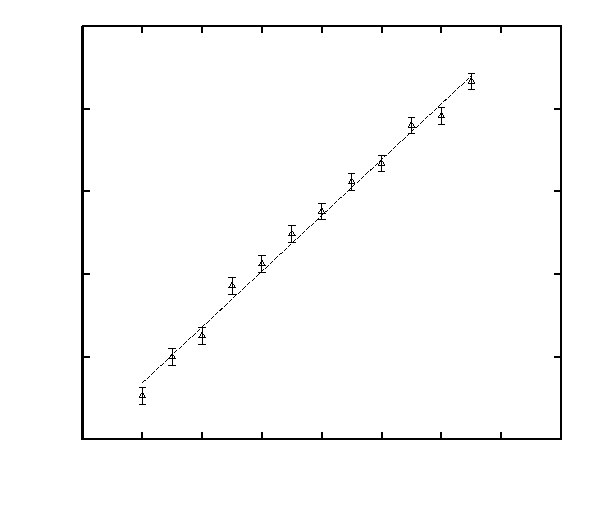
\includegraphics{least_squares}}%
    \gplfronttext
  \end{picture}%
\endgroup

\raisebox{4.55cm}{
\stdtablenocenter{3}
{$t$ (s) & $x$ (m) & $\Delta x$ (m)}
{$0.00$ & $1.57$ & $0.30$ \\
$0.10$ & $2.99$ & $0.30$ \\
$0.20$ & $3.75$ & $0.30$ \\
$0.30$ & $5.57$ & $0.30$ \\
$0.40$ & $6.36$ & $0.30$ \\
$0.50$ & $7.45$ & $0.30$ \\
$0.60$ & $8.27$ & $0.30$ \\
$0.70$ & $9.35$ & $0.30$ \\
$0.80$ & $10.01$ & $0.30$ \\
$0.90$ & $11.40$ & $0.30$ \\
$1.00$ & $11.74$ & $0.30$ \\
$1.10$ & $12.99$ & $0.30$ \\
}
}}
{Tabella dei dati relativi all'esempio \ref{esem:LeggeOrariaMinimiQuadrati}
e grafico relativo ai dati stessi. La retta di fit restituita da un fit
dei minimi quadrati \`e riportata sul grafico insieme ai punti
sperimentali.}
{fig:LeggeOrariaMinimiQuadrati}
I dati nella tabella sono stati simulati con un programma al calcolatore
assumendo che l'oggetto si muova lungo l'asse $x$ di moto rettilineo
uniforme:
$$
x(t) = x_0 + v_0 t
$$
con
\begin{eqnarray*}
x_0 & = & 2.3 \m\\
v_0 & = & 10 \m/{\rm s}
\end{eqnarray*}
ed ancora assumendo un errore di misura gaussiano sulle lunghezze con
deviazione standard pari a $0.3 \m$.
Le misure di tempo possono essere considerate abbastanza
accurate da far s\`i che la (\ref{eq:DeltaXTrascurabile}) sia verificata.

Notiamo esplicitamente che, avendo generato i dati al calcolatore, ci troviamo
nella posizione estremamente privilegiata di conoscere il valore dei
misurandi $x_0$ e $v_0$; cosa che, per ovvie ragioni, non \`e
di norma vera in laboratorio.
Questo ci permette di verificare in modo diretto la correttezza di un
dato algoritmo di analisi ed \`e un procedimento usato molto comunemente
nel progetto di esperimenti scientifici.

Applicando dunque i risultati appena derivati, un fit dei minimi quadrati
(abbiamo gi\`a verificato che le ipotesi necessarie siano verificate)
restituisce i seguenti valori:
\begin{eqnarray*}
x_0 & = & 2.05 \pm 0.16 \m\\
v_0 & = & 10.14 \pm 0.25 \m/{\rm s}\\
\end{eqnarray*}

che sono statisticamente compatibili (entro due $\sigma$) con i
valori dei misurandi, noti a priori.}

\end{exemplify}

\section{Metodo del minimo \texorpdfstring{$\chi^2$}{chi2}}

\index{minimo $\chi^2$!metodo di fit del}Supponiamo adesso che le incertezze
$\Delta y_i$ associate alle nostre misure siano, in generale, tutte diverse,
mentre manteniamo, per il momento, l'ipotesi che l'errore sulle $x_i$ sia
molto piccolo, nel senso della (\ref{eq:DeltaXTrascurabile}).
Il metodo dei minimi quadrati introdotto nel paragrafo precedente
pu\`o essere generalizzato a questa situazione introducendo
le quantit\`a:
$$
D_i = \frac{y_i - f(x; p_1 \ldots p_m)}{\Delta y_i}
$$
in cui ogni differenza viene {\itshape pesata} con l'inverso dell'errore
sulle misure $y_i$ (intuitivamente: maggiore \`e l'errore di misura,
minore \`e il peso che la misura stessa ha nel fit).
Si cercher\`a poi il minimo della funzione:
\eqnlbox{
S = \sum_{i=1}^n D_i^2 =
\sum_{i=1}^n\left[\frac{y_i - f(x; p_1 \ldots p_m)}{\Delta y_i}\right]^2
}{eq:SMinimoChiQuadro}
imponendo che le derivate rispetto a tutti i parametri siano nulle:
\eqn{
\left \{ \begin{array}{l}
\pfder{S}{p_1} = \pfder{}{p_1} \sum_{i=1}^n
\left[\frac{y_i - f(x; p_1 \ldots p_m)}{\Delta y_i}\right]^2 = 0\\
\pfder{S}{p_2} = \pfder{}{p_2} \sum_{i=1}^n
\left[\frac{y_i - f(x; p_1 \ldots p_m)}{\Delta y_i}\right]^2 = 0\\
\cdots \\
\pfder{S}{p_m} = \pfder{}{p_m} \sum_{i=1}^n
\left[\frac{y_i - f(x; p_1 \ldots p_m)}{\Delta y_i}\right]^2 = 0
\end{array} \right.
}

Questo metodo viene indicato come {\em il metodo del minimo $\chi^2$}.
Infatti se si assume che le $y_i$ abbiano una distribuzione gaussiana, le
$D_i$ sono variabili gaussiane con media zero e varianza uno ed $S$ \`e
una variabile che ha la distribuzione del $\chi^2$.


\subsection{Fit del minimo \texorpdfstring{$\chi^2$}{chi2} per una funzione
  costante: la media pesata}

\index{media pesata}
Supponiamo di eseguire un certo numero $n$ di misure {\itshape indipendenti}
di una stessa grandezza $y$ ottenendo $n$ valori $y_i$, in generali diversi
tra loro, con relative incertezze $\Delta y_i$, che pure ammettiamo poter
essere diverse tra di loro.
Ci poniamo il problema di valutare, a partire dai nostri dati,
la migliore stima per $y$ e l'incertezza associata.
Se potessimo trattare le misure tutte allo stesso modo (cio\`e se i
$\Delta y_i$
fossero tutti uguali), la migliore stima per $y$ sarebbe costituita dalla
media aritmetica delle $y_i$ (cfr. sezione \ref{subsec:FitMinQuadCostante}).
Ma se questa ipotesi cade \`e ragionevole aspettarsi, intuitivamente,
che le misure affette da incertezza maggiore debbano {\itshape contare}
meno delle altre.
Il problema si riduce, nel nostro linguaggio, ad un fit del minimo $\chi^2$
con una funzione costante:
$$
y = f(x; a)={\rm cost}=a
$$
Notiamo, per inciso, che la condizione (\ref{eq:DeltaXTrascurabile})
\`e qui automaticamente soddisfatta in quanto
$$
\tfdereval{f}{x}{x} = 0
$$
Costruiamo allora la somma:
$$
S = \sum_{i=1}^{n}\left(\frac{y_i-a}{\Delta y_i}\right)^2
$$
ed imponiamo che la derivata rispetto all'unico parametro sia nulla:
$$
\pfder{S}{a}=-2 \sum_{i=1}^{n} \frac{1}{\Delta y_i} \cdot
\left(\frac{y_i-a}{\Delta y_i}\right) = 0
$$
Questo fornisce:
$$
\sum_{i=1}^{n} \frac{y_i}{(\Delta y_i)^2} =
\sum_{i=1}^{n} \frac{a}{(\Delta y_i)^2} =
a \sum_{i=1}^{n} \frac{1}{(\Delta y_i)^2}
$$
ed infine:
\eqnlbox{
a = \frac{\displaystyle \sum_{i=1}^{n}
\frac{y_i}{(\Delta y_i)^2}}
{\displaystyle \sum_{i=1}^{n} \frac{1}{(\Delta y_i)^2}}
}{eq:MediaPesata}
L'incertezza associata si valuta come di consueto:
$$
(\Delta a)^2 = \sum_{i=1}^{n} \left(\pfder{a}{y_i}\right)^2 (\Delta y_i)^2 =
\frac{\displaystyle \sum_{i=1}^{n} \frac{1}{(\Delta y_i)^4}
\cdot (\Delta y_i)^2}
{\displaystyle \left[ \sum_{i=1}^{n} \frac{1}{(\Delta y_i)^2} \right]^2}=
\frac{\displaystyle \sum_{i=1}^{n} \frac{1}{(\Delta y_i)^2}}
{\displaystyle \left[ \sum_{i=1}^{n} \frac{1}{(\Delta y_i)^2} \right]^2}
$$
per cui:
\eqnlbox{
\Delta a = \frac{\displaystyle 1}
{\sqrt{\displaystyle \sum_{i=1}^{n} \frac{1}{(\Delta y_i)^2}}}}
{eq:ErroreMediaPesata}

\begin{exemplify}

\example{\label{esem:MediaPesata}
Si eseguono $5$ misure indipendenti dell'indice di rifrazione
dell'acqua ottenendo i risultati in tabella%
\footnote{
Dati realmente ottenuti negli anni accademici 2002-03, 2003-04, 2004-05.
}%
.
\stdtable{2}%
{$n_i$ & $\Delta n_i$}%
{$1.325$ & $0.012$\\
$1.3$ & $0.1$\\
$1.33$ & $0.01$\\
$1.331$ & $0.005$\\
$1.335$ & $0.006$\\}
Si vogliono combinare questi dati in modo da fornire una stima
statisticamente corretta di n. Assumendo che le incertezze riportate in
tabella siano state valutate correttamente e che gli effetti sistematici
siano stati tenuti sotto controllo, il modo corretto di procedere \`e quello
di eseguire una media pesata, secondo le equazioni (\ref{eq:MediaPesata}) e
(\ref{eq:ErroreMediaPesata}):
$$
n = 1.332 \pm 0.003
$$
Notiamo esplicitamente che la media aritmetica degli $n_i$ sarebbe
$1.324$, che \`e significativamente pi\`u bassa della media pesata
(sostanzialmente essa \`e influenzata dal valore della seconda misura che,
essendo affetta da un'incertezza relativa molto pi\`u grande degli altri,
conta meno nella media pesata).}

\end{exemplify}


\subsection{Fit del minimo \texorpdfstring{$\chi^2$}{chi2} nel caso lineare}
\label{sec:MinChiQuadroLineare}

In analogia alla sezione \ref{subsec:FitMinQuadLineare} applichiamo il
metodo del minimo $\chi^2$ al caso lineare:
$$
y = f(x; a, b) = a + b x
$$
Cominciamo dal costruire la somma:
$$
S = \sum_{i=1}^n\left(\frac{y_i - a - b x_i}{\Delta y_i}\right)^2
$$
e deriviamo rispetto ai parametri:
$$
\left \{ \begin{array}{l}
\pfder{S}{a} = -2\sum_{i=1}^{n} \frac{1}{\Delta y_i} \cdot
\left(\frac{y_i-a-b x_i}{\Delta y_i}\right) = 0\\
\pfder{S}{b} = -2\sum_{i=1}^{n} \frac{1}{\Delta y_i} \cdot
\left(\frac{y_i-a-b x_i}{\Delta y_i}\right)x_i = 0
\end{array} \right.
$$
da cui:
$$
\left \{ \begin{array}{l}
\displaystyle a \sum_{i=1}^{n} \frac{1}{(\Delta y_i)^2}
+ b \sum_{i=1}^{n} \frac{x_i}{(\Delta y_i)^2} =
\sum_{i=1}^{n} \frac{y_i}{(\Delta y_i)^2}\\
\displaystyle a \sum_{i=1}^{n} \frac{x_i}{(\Delta y_i)^2}
+ b \sum_{i=1}^{n} \frac{x_i^2}{(\Delta y_i)^2} =
\sum_{i=1}^{n} \frac{x_i y_i}{(\Delta y_i)^2}
\end{array} \right.
$$
Si ha infine:
\eqnbox{
\left \{ \begin{array}{l}
a=\frac{\displaystyle \sum_{i=1}^{n} \frac{y_i}{(\Delta y_i)^2}\cdot
\sum_{i=1}^{n} \frac{x_i^2}{(\Delta y_i)^2}
-\sum_{i=1}^{n} \frac{x_i}{(\Delta y_i)^2}\cdot
\sum_{i=1}^{n} \frac{x_i y_i}{(\Delta y_i)^2}}
{\displaystyle\sum_{i=1}^{n} \frac{1}{(\Delta y_i)^2}\cdot
\sum_{i=1}^{n} \frac{x_i^2}{(\Delta y_i)^2}-
\left(\sum_{i=1}^{n} \frac{x_i}{(\Delta y_i)^2}\right)^2} \\
\\
b=\frac{\displaystyle\sum_{i=1}^{n} \frac{1}{(\Delta y_i)^2}\cdot
\sum_{i=1}^{n} \frac{x_i y_i}{(\Delta y_i)^2}
-\sum_{i=1}^{n} \frac{y_i}{(\Delta y_i)^2}\cdot
\sum_{i=1}^{n} \frac{x_i}{(\Delta y_i)^2}}
{\displaystyle\sum_{i=1}^{n} \frac{1}{(\Delta y_i)^2}\cdot
\sum_{i=1}^{n} \frac{x_i^2}{(\Delta y_i)^2}-
\left(\sum_{i=1}^{n} \frac{x_i}{(\Delta y_i)^2}\right)^2}
\end{array} \right.}
ed ancora:
$$
\left \{ \begin{array}{l}
(\Delta a)^2=
\displaystyle\sum_{i=1}^{n}\left(\pfder{a}{y_i}\right)^2
\cdot (\Delta y_i)^2=
\frac{\displaystyle\sum_{i=1}^{n} \frac{x_i^2}{(\Delta y_i)^2}}
{\displaystyle\sum_{i=1}^{n} \frac{1}{(\Delta y_i)^2}\cdot
\sum_{i=1}^{n} \frac{x_i^2}{(\Delta y_i)^2}-
\left(\sum_{i=1}^{n} \frac{x_i}{(\Delta y_i)^2}\right)^2} \\
\\
(\Delta b)^2=
\displaystyle\sum_{i=1}^{n}\left(\pfder{b}{y_i}\right)^2
\cdot (\Delta y_i)^2=
\frac{\displaystyle\sum_{i=1}^{n} \frac{1}{(\Delta y_i)^2}}
{\displaystyle\sum_{i=1}^{n} \frac{1}{(\Delta y_i)^2}\cdot
\sum_{i=1}^{n} \frac{x_i^2}{(\Delta y_i)^2}-
\left(\sum_{i=1}^{n} \frac{x_i}{(\Delta y_i)^2}\right)^2}
\end{array} \right.
$$
da cui:
\eqnbox{
\left \{ \begin{array}{l}
\Delta a =
\frac{\sqrt{\displaystyle\sum_{i=1}^{n} \frac{x_i^2}{(\Delta y_i)^2}}}
{\sqrt{\displaystyle\sum_{i=1}^{n} \frac{1}{(\Delta y_i)^2}\cdot
\sum_{i=1}^{n} \frac{x_i^2}{(\Delta y_i)^2}-
\left(\sum_{i=1}^{n} \frac{x_i}{(\Delta y_i)^2}\right)^2}}\\
\\
\Delta b =
\frac{\sqrt{\displaystyle\sum_{i=1}^{n} \frac{1}{(\Delta y_i)^2}}}
{\sqrt{\displaystyle\sum_{i=1}^{n} \frac{1}{(\Delta y_i)^2}\cdot
\sum_{i=1}^{n} \frac{x_i^2}{(\Delta y_i)^2}-
\left(\sum_{i=1}^{n} \frac{x_i}{(\Delta y_i)^2}\right)^2}}
\end{array} \right.
}

\begin{exemplify}

\example{\label{esem:LeggeOrariaMinimoChiQuadro}I dati nella tabella
sono stati simulati con lo stesso programma dell'esempio
\ref{esem:LeggeOrariaMinimiQuadrati} con una piccola variante:
questa volta gli errori di misura sulle lunghezze non sono costanti
ma direttamente proporzionali alle lunghezze stesse, di modo che
l'errore relativo \`e costante e pari al $5\%$ (cfr. figura
\ref{fig:LeggeOrariaMinChiQuadro}).
\panelfig{
% GNUPLOT: LaTeX picture with Postscript
\begingroup
\footnotesize
  \makeatletter
  \providecommand\color[2][]{%
    \GenericError{(gnuplot) \space\space\space\@spaces}{%
      Package color not loaded in conjunction with
      terminal option `colourtext'%
    }{See the gnuplot documentation for explanation.%
    }{Either use 'blacktext' in gnuplot or load the package
      color.sty in LaTeX.}%
    \renewcommand\color[2][]{}%
  }%
  \providecommand\includegraphics[2][]{%
    \GenericError{(gnuplot) \space\space\space\@spaces}{%
      Package graphicx or graphics not loaded%
    }{See the gnuplot documentation for explanation.%
    }{The gnuplot epslatex terminal needs graphicx.sty or graphics.sty.}%
    \renewcommand\includegraphics[2][]{}%
  }%
  \providecommand\rotatebox[2]{#2}%
  \@ifundefined{ifGPcolor}{%
    \newif\ifGPcolor
    \GPcolorfalse
  }{}%
  \@ifundefined{ifGPblacktext}{%
    \newif\ifGPblacktext
    \GPblacktexttrue
  }{}%
  % define a \g@addto@macro without @ in the name:
  \let\gplgaddtomacro\g@addto@macro
  % define empty templates for all commands taking text:
  \gdef\gplbacktext{}%
  \gdef\gplfronttext{}%
  \makeatother
  \ifGPblacktext
    % no textcolor at all
    \def\colorrgb#1{}%
    \def\colorgray#1{}%
  \else
    % gray or color?
    \ifGPcolor
      \def\colorrgb#1{\color[rgb]{#1}}%
      \def\colorgray#1{\color[gray]{#1}}%
      \expandafter\def\csname LTw\endcsname{\color{white}}%
      \expandafter\def\csname LTb\endcsname{\color{black}}%
      \expandafter\def\csname LTa\endcsname{\color{black}}%
      \expandafter\def\csname LT0\endcsname{\color[rgb]{1,0,0}}%
      \expandafter\def\csname LT1\endcsname{\color[rgb]{0,1,0}}%
      \expandafter\def\csname LT2\endcsname{\color[rgb]{0,0,1}}%
      \expandafter\def\csname LT3\endcsname{\color[rgb]{1,0,1}}%
      \expandafter\def\csname LT4\endcsname{\color[rgb]{0,1,1}}%
      \expandafter\def\csname LT5\endcsname{\color[rgb]{1,1,0}}%
      \expandafter\def\csname LT6\endcsname{\color[rgb]{0,0,0}}%
      \expandafter\def\csname LT7\endcsname{\color[rgb]{1,0.3,0}}%
      \expandafter\def\csname LT8\endcsname{\color[rgb]{0.5,0.5,0.5}}%
    \else
      % gray
      \def\colorrgb#1{\color{black}}%
      \def\colorgray#1{\color[gray]{#1}}%
      \expandafter\def\csname LTw\endcsname{\color{white}}%
      \expandafter\def\csname LTb\endcsname{\color{black}}%
      \expandafter\def\csname LTa\endcsname{\color{black}}%
      \expandafter\def\csname LT0\endcsname{\color{black}}%
      \expandafter\def\csname LT1\endcsname{\color{black}}%
      \expandafter\def\csname LT2\endcsname{\color{black}}%
      \expandafter\def\csname LT3\endcsname{\color{black}}%
      \expandafter\def\csname LT4\endcsname{\color{black}}%
      \expandafter\def\csname LT5\endcsname{\color{black}}%
      \expandafter\def\csname LT6\endcsname{\color{black}}%
      \expandafter\def\csname LT7\endcsname{\color{black}}%
      \expandafter\def\csname LT8\endcsname{\color{black}}%
    \fi
  \fi
  \setlength{\unitlength}{0.0500bp}%
  \begin{picture}(5760.00,4888.80)%
    \gplgaddtomacro\gplbacktext{%
      \csname LTb\endcsname%
      \put(660,660){\makebox(0,0)[r]{\strut{} 0}}%
      \put(660,1453){\makebox(0,0)[r]{\strut{} 3}}%
      \put(660,2246){\makebox(0,0)[r]{\strut{} 6}}%
      \put(660,3039){\makebox(0,0)[r]{\strut{} 9}}%
      \put(660,3832){\makebox(0,0)[r]{\strut{} 12}}%
      \put(660,4625){\makebox(0,0)[r]{\strut{} 15}}%
      \put(792,440){\makebox(0,0){\strut{}-0.2}}%
      \put(1366,440){\makebox(0,0){\strut{} 0}}%
      \put(1940,440){\makebox(0,0){\strut{} 0.2}}%
      \put(2515,440){\makebox(0,0){\strut{} 0.4}}%
      \put(3089,440){\makebox(0,0){\strut{} 0.6}}%
      \put(3663,440){\makebox(0,0){\strut{} 0.8}}%
      \put(4237,440){\makebox(0,0){\strut{} 1}}%
      \put(4812,440){\makebox(0,0){\strut{} 1.2}}%
      \put(5386,440){\makebox(0,0){\strut{} 1.4}}%
      \put(220,2642){\rotatebox{90}{\makebox(0,0){\strut{}\gplabel{$x\;({\rm m})$}}}}%
      \put(3089,110){\makebox(0,0){\strut{}\gplabel{$t\;({\rm s})$}}}%
    }%
    \gplgaddtomacro\gplfronttext{%
    }%
    \gplbacktext
    \put(0,0){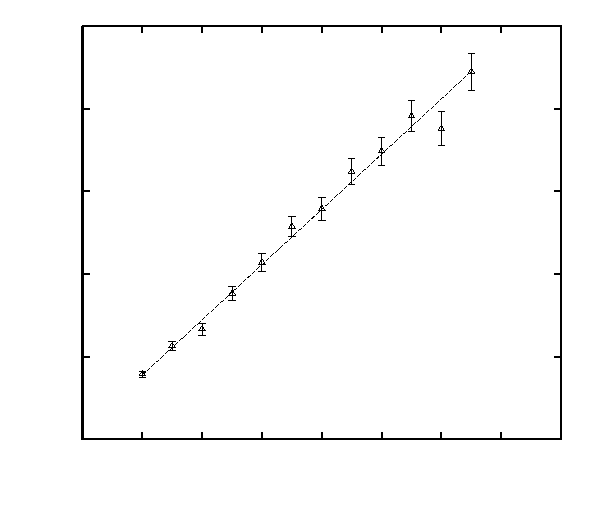
\includegraphics{least_chisquare}}%
    \gplfronttext
  \end{picture}%
\endgroup

\raisebox{4.55cm}{
\stdtablenocenter{3}
{$t$ (s) & $x$ (m) & $\Delta x$ (m)}
{$0.00$ & $2.36$ & $0.11$ \\
$0.10$ & $3.38$ & $0.17$ \\
$0.20$ & $4.00$ & $0.21$ \\
$0.30$ & $5.30$ & $0.27$ \\
$0.40$ & $6.42$ & $0.32$ \\
$0.50$ & $7.72$ & $0.36$ \\
$0.60$ & $8.37$ & $0.42$ \\
$0.70$ & $9.71$ & $0.47$ \\
$0.80$ & $10.46$ & $0.52$ \\
$0.90$ & $11.73$ & $0.57$ \\
$1.00$ & $11.27$ & $0.62$ \\
$1.10$ & $13.34$ & $0.67$ \\
}
}}
{Tabella dei dati relativi all'esempio \ref{esem:LeggeOrariaMinimoChiQuadro}
e grafico relativo ai dati stessi. La retta di fit restituita da un fit
del minimo $\chi^2$ \`e riportata sul grafico insieme ai punti sperimentali.}
{fig:LeggeOrariaMinChiQuadro}

Ammettendo di nuovo che gli errori sulle misure di tempo siano
trascurabili, secondo la (\ref{eq:DeltaXTrascurabile}), siamo nelle ipotesi
del minimo $\chi^2$. Il fit del minimo $\chi^2$ in effetti fornisce per
i parametri i seguenti valori:
\begin{eqnarray*}
x_0 & = & 2.33 \pm 0.09 \\
v_0 & = & 10.03 \pm 0.28 \\
\end{eqnarray*}

che di nuovo sono compatibili con i misurandi.

Se avessimo applicato il metodo dei minimi quadrati---procedimento
statisticamente non corretto, in questo caso, dato che gli errori di misura
sono diversi tra loro---avremmo ottenuto:
\begin{eqnarray*}
x_0 & = & 2.41 \pm 0.06 \m\\
v_0 & = & 9.87 \pm 0.10 \m/{\rm s}\\
\end{eqnarray*}

In questo caso le stime dei parametri sono leggermente peggiori (come \`e
logico aspettarsi), sia pure ancora ragionevoli; gli errori sui parametri
stessi, viceversa, sono un artefatto del fit e non devono essere presi
seriamente.}

\end{exemplify}


\section{Fit di tipo generale}
Nei metodi finora discussi abbiamo sempre supposto che l'errore sulle $x_i$
fosse trascurabile, e come tale l'abbiamo trattato. Finora ci siamo quindi
occupati di casi relativamente semplici. Relativamente, s'intende, al caso
che esamineremo adesso: vogliamo infatti studiare il problema di fitting nel
caso pi\`u generale in cui non sono trascurabili n\'e gli errori su $y$ n\'e
quelli su $x$.

Il primo problema che si incontra \`e che in un'equazione del tipo
$y = f(x; p_1 \ldots p_m)$ non \`e chiaro quale sia il valore da usare per
$x$ in modo da calcolare il valore teorico di $y$ e quindi cercare i migliori
valori dei parametri che soddisfino la richiesta di rendere minimo il $\chi^2$.
Non conoscendo $x$ il problema \`e quindi concettualmente pi\`u
complicato: bisogna determinare i valori di $(\tilde{x_i}, \tilde{y_i})$
tali che sia minimo
\eqn{
\sum_{i=1}^n\left[\left(\frac{\tilde{x_i}-x_i}{\Delta x_i}\right)^2 +
\left(\frac{\tilde{y_i}-y_i}{\Delta y_i}\right)^2\right]
}
con la condizione che
\eqn{
{\cal F}(\tilde{x_i}, \tilde{y_i}; \, p_1 \ldots p_m)=0
\qquad\forall i= 1\ldots n
}
dove ${\cal F}(x, y; \, p_1 \ldots p_m)$  \`e la relazione che si
vuole che leghi la $x$ alla $y$ scritta in forma implicita.

Si tratta di un problema di minimo condizionato: usando il metodo dei
{\itshape moltiplicatori di Lagrange} ci si riduce al problema seguente:
minimizzare
\eqnl{
S = \sum_{i=1}^n\left[\left(\frac{\tilde{x_i}-x_i}{\Delta x_i}\right)^2+
\left(\frac{\tilde{y_i}-y_i}{\Delta y_i}\right)^2+
\lambda_i {\cal F}(\tilde{x_i}, \tilde{y_i}; \, p_1 \ldots p_m)\right]
}{eq:SGenerale}
Le cose da determinare sono $\tilde{x_i}$, $\tilde{y_i}$, $\lambda_i$,
$p_1 \ldots p_m$: in tutto $3n+m$;
ci sono quindi derivate parziali rispetto a $3n+m$ variabili.

Il problema si pu\`o risolvere nel caso pi\`u generale solo con metodi
numerici approssimati.
Diamo alcuni cenni sulla tecnica di risoluzione:
\begin{numlist}
\item{
Il primo passo \`e di conoscere un valore approssimato dei parametri.
}
\item{
Il secondo passo \`e di usare invece di  ${\cal F}(x, y; \, p_1 \ldots p_m)$
la sua approssimazione al prim'ordine. Pertanto ad 
${\cal F}(x, y; \, p_1 \ldots p_m)$ viene sostituita una funzione lineare.
}
\item{
Quindi c'\`e una certa quantit\`a di algebra, sostituzioni, ecc.
}
\item{
Il risultato \`e un sistema di equazioni lineari che dicono di quanto
devono essere corrette le stime iniziali dei parametri.
}
\item{
A questo punto si procede con metodo iterativo, cio\`e si prendono i
nuovi valori dei parametri e si ricomincia.
}
\item{
Se il processo converge alla fine si ottengono i valori richiesti
per i parametri.
}
\end{numlist}

\begin{exemplify}

\example{Analizziamo in dettaglio la procedura generale di fit nel caso
puramente lineare%
\footnote{Per le funzioni che, come questa, sono lineari nei parametri,
potrebbero essere usati metodi pi\`u semplici (provate).
Tuttavia la semplicit\`a dell'esempio permette di seguire
meglio la tecnica proposta.}%
:
$$
y = f(x; \, p) = p x
$$
La forma implicita della funzione che lega la $y$ alla $x$ si scrive come:
$$
{\cal F}(x, y; \, p) = y - p x = 0
$$
Costruiamo allora la somma (\ref{eq:SGenerale}):
$$
S = \sum_{i=1}^n\left[\left(\frac{\tilde{x_i} - x_i}{\Delta x_i}\right)^2+
\left(\frac{\tilde{y_i} - y_i}{\Delta y_i}\right)^2 +
\lambda_i(\tilde{y_i} - p\tilde{x_i})\right]
$$
Le condizioni di minimo sono:
$$
\left\{\begin{array}{l}
\pfder{S}{\tilde{x_i}}=\frac{2(\tilde{x_i}-x_i)}{(\Delta x_i)^2}-\lambda_i p=0
\vspace{0.2cm}\\
\pfder{S}{\tilde{y_i}}=\frac{2(\tilde{y_i}-y_i)}{(\Delta y_i)^2}-\lambda_i=0
\vspace{0.2cm}\\
\pfder{S}{\lambda_i}=\tilde{y_i} - p\tilde{x_i} = 0
\vspace{0.2cm}\\
\pfder{S}{p} = - \dsum{\lambda_i \tilde{x_i}}{i}{1}{n} \approx
- \dsum{\lambda_i x_i}{i}{1}{n} = 0
\end{array}\right.
$$
Dove nell'ultima relazione si \`e linearizzata la $\cal F$.
Si ricavano $\tilde{x_i}$ ed $\tilde{y_i}$ dalle prime due relazioni:
$$
\left\{\begin{array}{l}
\displaystyle \tilde{x_i} = \frac{\lambda_i p \cdot (\Delta x_i)^2}{2} + x_i
\vspace{0.2cm}\\
\displaystyle \tilde{y_i} = \frac{\lambda_i \cdot (\Delta y_i)^2}{2} + y_i
\end{array}\right.
$$
e si sostituiscono nella terza:
$$
\frac{\lambda_i \cdot (\Delta y_i)^2}{2} + y_i -
\frac{\lambda_i p^2 \cdot (\Delta x_i)^2}{2} - x_i = 0
$$
da cui si ricava $\lambda_i$:
$$
\lambda_i = \frac{2(y_i - p x_i)}{p^2 \cdot (\Delta x_i)^2 + (\Delta y_i)^2}
$$
che, sostituito nella quarta relazione d\`a:
\eqnl{
p'=\frac{\displaystyle
\dsum{\frac{x_i y_i}{p^2 \cdot (\Delta x_i)^2 + (\Delta y_i)^2}}{i}{1}{n}}
{\displaystyle
\dsum{\frac{x_i^2}{p^2 \cdot (\Delta x_i)^2 + (\Delta y_i)^2}}{i}{1}{n}}
}{eq:FitGeneraleRetta}
a questo punto entra in funzione il metodo iterativo: si stima $p$ (ad esempio
dal grafico) e si usa questa stima nel secondo membro della
(\ref{eq:FitGeneraleRetta}) ottenendo un nuovo $p$ (chiamato $p'$), si ripete
il procedimento fino a quando la differenza fra i successivi valori di $p$ \`e
entro l'errore su $p$.

Per stimare gli errori su $p$ si usano l'equazione (\ref{eq:FitGeneraleRetta})
e le tecniche della propagazione degli errori ed il valore stimato di $p$:
$$
(\Delta p)^2=
\dsum{\left[\left(\pfder{p}{x} \cdot \Delta x_i \right)^2+
\left(\pfder{p}{y} \cdot \Delta y_i \right)^2 \right]}{i}{1}{n}
 =\frac{1}{\displaystyle\sum_{i=1}^{n}\frac{x_i^2}{p^2\cdot(\Delta x_i)^2 +
(\Delta y_i)^2}}
$$}

\end{exemplify}


\section{Test del \texorpdfstring{$\chi^2$}{chi2}}
\label{sec:TestChiQuadro}


\index{$\chi^2$!test del}Richiamiamo la definizione della variabile $\chi^2$ a
$n$ gradi di libert\`a: date $n$ variabili $x_i$ gaussiane con media $\mu_i$ e
deviazione standard $\sigma_i$ e costruite le variabili standard
$$
z_i=\frac{x_i-\mu_i}{\sigma_i}
$$
la quantit\`a
\eqn{
S=\sum_{i=1}^n z_i^2 = \sum_{i=1}^n\left(\frac{x_i-\mu_i}{\sigma_i}\right)^2
}
\`e distribuita secondo la funzione di distribuzione del $\chi^2$
ad $n$ gradi di libert\`a, che \`e data dalla (\ref{eq:ChiQuadro}).
La media e la varianza valgono rispettivamente:
\begin{eqnarray*}
\mu_S &=&n\\
\sigma_S^2&=&2n
\end{eqnarray*}

Fissato il numero di gradi di libert\`a $n$, le tavole riportate nelle
appendici \ref{app:ChiQuadro1} e \ref{app:ChiQuadro2} forniscono
il valore $\gamma$ per cui la probabilit\`a che $S$ sia
minore di $\gamma$ sia uguale ad un certo valore $\wp$:
$$
\prob{S\le\gamma} = \wp
$$

\begin{exemplify}

\example{Sia $n=10$; ci si domanda quale sia il valore $\gamma$ tale che:
$$
\prob{S \le \gamma} = 95\%
$$
Il risultato si legge direttamente nella tavola in appendice
\ref{app:ChiQuadro1} ed \`e:
$$
\gamma = 18.308
$$}

\end{exemplify}


\subsection{Test del \texorpdfstring{$\chi^2$}{chi2} per una serie di misure}

Il $\chi^2$ pu\`o fornire un criterio generale ed obiettivo per decidere
se una certa equazione o una certa legge descriva bene oppure no i risultati
sperimentali.
Supponiamo, al solito, di aver misurato le quantit\`a $(x_i, y_i)$ legate
tra di loro da una funzione $y = f(x; p_1 \ldots p_m)$, la cui forma viene
ipotizzata in base a considerazioni fisiche, ed i cui parametri
$p_1 \ldots p_m$ sono determinati con uno dei metodi di fit discussi prima,
per esempio il metodo dei minimi quadrati o del minimo $\chi^2$.
Il $\chi^2$ in questo caso vale
$$
S=\sum_{i=1}^n \left[
\frac{y_i - f(x_i; p_1 \ldots p_m)}{\Delta y_i} \right]^2
$$
La quantit\`a $S$ viene spesso indicata con il nome di \emph{somma dei
residui}; intuitivamente \`e chiaro che, quanto pi\`u $S$ \`e grande, tanto
pi\`u la curva teorica si discosta dai punti sperimentali.

Supposto che gli errori siano stati valutati in modo corretto, andiamo a vedere
qual \`e il significato da attribuire al numero $S$.
Si cerca sulle tavole in corrispondenza al numero di gradi di libert\`a
dove si trova il valore $S$. Quando si fa un fit il numero di gradi di
libert\`a $\nu$ \`e il numero $n$ delle misure meno il numero $m$ di parametri
della funzione $f(x; p_1 \ldots p_m)$
\eqnl{
\nu=n-m
}{eq:nGradiDiLiberta}

\begin{exemplify}

\example{Supponiamo di aver ottenuto $S=7.2$ con $\nu=5$.
Dalla tavola in appendice \ref{app:ChiQuadro1} si ottiene:
$$
\prob{\chi^2\le S} \approx 80\%
$$
Questo significa che ripetendo le misure tante volte
ci si aspetta che nell'$80\%$ dei casi si otterr\`a un valore minore
di $7.2$; cio\`e $7.2$ \`e un valore non molto buono per il $\chi^2$,
ma nemmeno assurdo, nel $20\%$ dei casi pu\`o succedere che venga un risultato
pi\`u alto.

Per inciso: $\prob{\chi^2\ge S}$ viene solitamente chiamato livello di
significativit\`a ed \`e ovviamente:
$$
\prob{\chi^2\ge S} = 1 - \prob{\chi^2\le S}
$$}

\example{Nel caso dell'esempio \ref{esem:LeggeOrariaMinimiQuadrati} il
valore di $S$ restituito dal fit vale:
$$
S = 12.47 \qquad (\nu = 10)
$$

Il livello di significativit\`a del fit \`e dunque circa il $75 \%$, come
si legge in appendice \ref{app:ChiQuadro1}.}

\example{Nel caso dell'esempio \ref{esem:LeggeOrariaMinimoChiQuadro}
il valore di $S$ restituito dal fit del minimo $\chi^2$ vale:
$$
S = 8.00 \qquad (\nu = 10)
$$

mentre quello restituito dal fit dei minimi quadrati:
$$
S = 8.76 \qquad (\nu = 10)
$$

Il lettore non dovrebbe essere stupito dal fatto che $S$ sia
pi\`u piccolo nel caso del fit del minimo $\chi^2$ (i nomi non sono
in genere scelti a caso).}

\end{exemplify}

Convenzionalmente si accetta come limite $\prob{\chi^2\le S}$ per i risultati
buoni quello del $95\%$ da un lato, e quello del $5\%$ dall'altro, perch\'e,
anche se a prima vista sembra che la cosa migliore sia ottenere dei $\chi^2$
molto piccoli (o addirittura zero), in realt\`a questi casi vanno guardati con
sospetto. Di solito $\chi^2$ piccoli si ottengono perch\'e gli errori
sono sovrastimati, oppure i risultati sono truccati,
cio\`e lo sperimentatore (consciamente o no) tende ad attribuire al
risultato delle misure il valore che gli piacerebbe.
Esistono tuttavia altri livelli di significativit\`a a seconda dei
particolari problemi studiati. \`E comunque buona regola indicare sempre
quale \`e il valore del $\chi^2$ ottenuto e quindi la probabilit\`a del
$\chi^2$ associata alle ipotesi fatte ed ai parametri dedotti dalle misure.


\subsection{Test del \texorpdfstring{$\chi^2$}{chi2} per una distribuzione}

Supponiamo di fare un esperimento che abbia come oggetto l'osservazione
di $n$ possibili eventi $E_1 \ldots E_n$ e registriamo le
occorrenze $o_1 \ldots o_n$ di ciascuno di questi possibili eventi%
\footnote{
Le occorrenze osservate vengono generalmente indicate con la lettera $o$
dall'inglese \emph{observed}, che significa appunto \emph{osservato}.
}%
.
D'altra parte possiamo fare certe ipotesi
sul fenomeno che stiamo studiando le quali ci permettono di determinare
le occorrenze teoriche%
\footnote{
Le occorrenze teoriche si indicano solitamente con la lettera $e$ dall'inglese
\emph{expected} che significa \emph{atteso}.
}
$e_1 \ldots e_n$. Ci saranno
differenze tra le occorrenze osservate e quelle teoriche. Per determinare
se le differenze sono significative (e quindi eventualmente rifiutare
le ipotesi che hanno portato a calcolare gli $e_i$) si usa la quantit\`a
\eqnl{
S = \sum_{i=1}^n\frac{(o_i-e_i)^2}{e_i}
}{eq:ChiQuadroDistribuzione}
che viene considerata ancora una variabile $\chi^2$.
Formalmente ricorda un $\chi^2$ perch\'e si suppone che sia Poissoniana la
distribuzione di ognuna delle occorrenze $o_i$: $e_i$ rappresenta il valor
medio della parent distribution  e per una variabile Poissoniana la varianza
coincide con la media, per cui $\sigma^2_{o_i} = e_i$.
\`E tuttavia importante ricordare che  $o_i$ ed $e_i$ non sono variabili
gaussiane; o meglio: lo sono soltanto in condizioni limite,
cio\`e per $o_i$ (e quindi $e_i$) grande. In queste condizioni la
(\ref{eq:ChiQuadroDistribuzione}) tende ad una variabile $\chi^2$; $o_i>3$
\`e una condizione sufficiente per la maggior parte dei casi
che si incontrano in pratica.

I {\itshape \em gradi di libert\`a} sono $n-m-1$ dove $n$ \`e il numero delle
classi (cio\`e il numero degli eventi possibili) ed $m$ \`e il numero dei
parametri che servono per calcolare le occorrenze teoriche
$e_1 \ldots e_n$; inoltre deve essere soddisfatta la seguente relazione:
$$
\sum_{i=1}^n o_i=N
$$
dove $N$ \`e il numero totale delle osservazioni,
e questa relazione causa la perdita di un ulteriore grado di libert\`a.
Nel limite in cui la quantit\`a (\ref{eq:ChiQuadroDistribuzione})
pu\`o essere considerata un $\chi^2$ ad essa si
attribuisce lo stesso significato probabilistico trattato precedentemente.

\begin{exemplify}

\example{Si supponga di avere un foglio di carta diviso in 64 quadrati
numerati (da $1$ a $64$).
Si prendono 64 dischi e si lasciano cadere sul foglio di carta
uno alla volta, in modo che si distribuiscano pressoch\'e uniformemente
sul quadrato. Quindi si fa una tavola suddividendo i quadrati in funzione
del numero dei dischi che essi contengono:
\stdtable{3}%
{$k$ & $o_k$ & $e_k$}%
{$0$ & $21$ & $23.54$\\
$1$ & $26$ & $23.54$\\
$2$ & $13$ & $11.77$\\
$3$ & $4$ & $3.22$\\
$4$ & $0$ & $0.38$\\}
Per calcolare le frequenze teoriche, si \`e fatta l'ipotesi che
la distribuzione della variabile $k$ sia una Poissoniana con media
$1$ ($64$ dischi in $64$ quadrati cio\`e in media un disco
per quadrato):
$$
\prob{k}=\frac{1^k}{k!}e^{-1}=\frac{1}{k!}\cdot \frac{1}{e}
$$
Le frequenze teoriche si calcolano moltiplicando $\prob{k}$ per il numero
totale $n=64$ dei quadrati:
$$
e_k=\frac{1}{k!} \cdot \frac{64}{e}
$$
Calcoliamo il valore $S$ del $\chi^2$:
\begin{eqnarray*}
S &=& \sum_{i=0}^3\frac{(o_i-e_i)^2}{e_i}=\\
&=& \frac{(21-23.54)^2}{23.54}+ \frac{(26-23.54)^2}{23.54}+
\frac{(13-11.77)^2}{11.77}+\frac{(4-5.15)^2}{5.15} \approx 0.91
\end{eqnarray*}
I gradi di libert\`a sono $4-0-1=3$ (qui nessun parametro \`e
stato ricavato dalle misure: questa \`e una Poissoniana limite di una
Binomiale in cui sia $n$ che $p$ sono noti). Utilizzando le tavole
si trova:
$$\prob{\chi^2\le S} \approx 22\%.$$\normalsize}

\example{\label{esem:Lotto}L'istogramma in figura \ref{fig:LottoBA}
si riferisce ai numeri del gioco del lotto usciti nella ruota di Bari dal
1937 ad oggi. Per ognuna delle possibili uscite $k$ ($k = 1 \ldots 90$) \`e
riportato il numero di volte in cui essa si \`e verificata.
\panelfig
{\onebyonetexfig{./pp_fit/figure/lotto_BA.tex}}
{Istogramma in frequenza delle uscite del gioco del lotto sulla ruota di Bari
dal $1937$ ad oggi.}
{fig:LottoBA}

I dati si riferiscono a 4223 estrazioni; ricordiamo che ogni volta vengono
estratti 5 numeri (senza rimpiazzo) per cui ogni numero ha una probabilit\`a
di essere estratto pari a $\frac{5}{90}$.
Se il gioco non \`e truccato ci aspettiamo che il numero medio $e_k$ di uscite
per il numero $k$ in 4223 estrazioni sia uguale per tutti e pari a:
$$
e_k = 4223 \cdot \frac{5}{90} \approx 234.6 \qquad k = 1\ldots 90
$$
Un test del $\chi^2$ su questa distribuzione restituisce una somma dei
residui pari a:
$$
S = 98.313
$$
Il numero di gradi di libert\`a \`e qui $\nu = 90 - 0 - 1$ per cui il
livello di significativit\`a \`e pari a circa il $75\%$.
Con i dati in nostro possesso dobbiamo accettare l'ipotesi che il gioco non
sia truccato (per lo meno nel senso del $\chi^2$).}


\end{exemplify}



\begin{exercises}

\exercise{Seguendo le sezioni \ref{subsec:FitMinQuadCostante} e
\ref{subsec:FitMinQuadLineare} ricavare con il metodo dei minimi quadrati
il miglior valore di $a$ per la funzione:
$$
f(x, a)=a x
$$}

\exercise{Seguendo le sezioni \ref{subsec:FitMinQuadCostante} e
\ref{subsec:FitMinQuadLineare} ricavare con il metodo dei minimi quadrati
il miglior valore di $a$ per la funzione:
$$
f(x, a)=a x^2
$$}

\exercise{Seguendo le sezioni \ref{subsec:FitMinQuadCostante} e
\ref{subsec:FitMinQuadLineare} ricavare con il metodo dei minimi quadrati
il miglior valore di $a$ per la funzione:
$$
f(x)=a e^{-x}
$$}

\exercise{Calcolare esplicitamente la media pesata (con relativa incertezza)
e la media aritmetica dei valori dell'indice di rifrazione dell'acqua
riportati nell'esempio \ref{esem:MediaPesata} e verificare che i
risultati dell'esempio stesso sono corretti.}

\exercise{Con riferimento all'esempio \ref{esem:LeggeOrariaMinimiQuadrati},
eseguire un fit dei minimi quadrati utilizzando i risultati ottenuti
nella sezione \ref{subsec:FitMinQuadLineare} e verificare che i risultati
coincidano con quelli forniti alla fine dell'esercizio stesso---i dati sono
riportati nella tabella in figura \ref{fig:LeggeOrariaMinimiQuadrati}.}

\exercise{Con riferimento all'esempio \ref{esem:LeggeOrariaMinimoChiQuadro},
eseguire un fit del minimo $\chi^2$ utilizzando i risultati ottenuti
nella sezione \ref{sec:MinChiQuadroLineare} e verificare che i
risultati coincidano con quelli forniti alla fine dell'esercizio
stesso---i dati sono riportati nella tabella in figura
\ref{fig:LeggeOrariaMinChiQuadro}.}

\exercise{Discutere se per i dati riportati nell'esercizio \ref{eser:Lavagna}
\`e accettabile l'ipotesi di distribuzione Gaussiana (qual \`e il livello di
significativit\`a).}

\end{exercises}

\chapter{Formule approssimate}
\mt

Trattiamo in questo capitolo alcuni problemi connessi alla
\emph{manipolazione} (integrazione, derivazione, interpolazione) di funzioni
tabulate---funzioni cio\`e di cui si conoscono i valori solamente in
un determinato numero di punti discreti dell'intervallo di variabilit\`a.


\section{Derivata di una funzione data per punti}

Supponiamo di conoscere i valori di una generica funzione $f(x)$ in
un certo numero di punti $x_i$ egualmente spaziati di una quantit\`a $h$.
Per fissare le idee supponiamo di avere una tabella con $2n + 1$ valori di
$f(x)$, in corrispondenza di:
$$
x_i = x_0 + i \cdot h \qquad i = -n \ldots n
$$
Supponiamo ancora che la funzione sia {\itshape derivabile} su tutto
l'intervallo delle $x$ a cui siamo interessati, e che $h$ sia abbastanza
piccolo in modo che la funzione non compia forti oscillazione
all'interno di ciascun intervallo $\cinterval{x_i}{x_{i+1}}$.
In queste condizioni avr\`a senso usare le formule approssimate che
ricaveremo.

Per semplicit\`a indicheremo nel seguito con $f_i$ il valore della funzione
nel punto $x_i$:
$$
f_i = f(x_i)
$$
ed useremo la seguente notazione per le derivate:
$$
\left \{ \begin{array}{l}
f'_i   = \tfdereval{f}{x}{x_i}
\vspace{0.3cm}\\
f''_i  = \tsdereval{f}{x}{x_i}
\vspace{0.3cm}\\
f'''_i = \tndereval{f}{x}{x_i}{3}
\vspace{0.3cm}\\
f^{iv}_i  = \tndereval{f}{x}{x_i}{4} 
\end{array} \right.
$$

Il valore $f_{i+m}$ di $f(x)$ in un generico punto $x_i + mh$ si pu\`o
esprimere in termini di $f(x)$ e delle sue derivate nel punto $x_i$
per mezzo di uno sviluppo in serie di Taylor intorno ad $x_i$:
$$
f_{i+m} = f(x_i + mh) = f_i + mhf'_i + \frac{(m h)^2}{2!} f''_i +
\frac{(m h)^3}{3!}f'''_i + \cdots
$$
Quindi per $m=1$ si ha:
$$
f_{i+1} = f(x_i + h) = f_i + h f'_i + \frac{h^2}{2}f''_i+
\frac{h^3}{6}f'''_i + \cdots
$$
da cui si pu\`o scrivere facilmente lo sviluppo completo per la derivata
di $f(x)$ in $x_i$:
$$
f'_i=\frac{f_{i+1}-f_i}{h}-
\left(\frac{h}{2}f''_i+\frac{h^2}{6}f'''_i+ \cdots\right)
$$
Trascurando i termini tra parentesi si ottiene un'espressione
{\itshape utilizzabile} per $f'_i$:
\eqnlbox{
\begin{array}{ll}
\displaystyle f'_i & \simeq
\frac{\displaystyle f_{i+1} - f_i}{\displaystyle h}
\vspace{0.3cm}\\
\displaystyle \Delta f'_i & \simeq -
\frac{\displaystyle h}{\displaystyle 2} f''_i
\end{array}
}{eq:DerivataApprossimata1}
dove per $\Delta f'_i$ si prende il primo dei termini tra parentesi,
che solitamente costituisce la correzione dominante allo sviluppo.

Per $m=-1$ si ottiene:
$$
f_{i-1} = f(x_i - h) = f_i-h f'_i + \frac{h^2}{2}f''_i -
\frac{h^3}{6}f'''_i + \cdots
$$
Sottraendo $f_{i-1}$ da $f_{i+1}$ si ottiene un'altra espressione approssimata
per la derivata prima:
\eqnlbox{
\begin{array}{ll}
\displaystyle f'_i & \simeq \frac{\displaystyle f_{i+1}-f_{i-1}}
{\displaystyle 2h}
\vspace{0.3cm}\\
\Delta f'_i & \simeq -\frac{\displaystyle h^2}{\displaystyle 6}f'''_i
\end{array}
}{eq:DerivataApprossimata2}

\noindent Sommando $f_{i+1}$ con $f_{i-1}$ si ottiene infine  un'espressione
approssimata per $f''_i$:
\eqnlbox{
\begin{array}{ll}
\displaystyle f''_i & \simeq \frac{\displaystyle f_{i+1}-2f_i+f_{i-1}}
{\displaystyle h^2}
\vspace{0.3cm}\\
\displaystyle \Delta f''_i & \simeq -\frac{\displaystyle h^2}
{\displaystyle 12}f^{iv}_i
\end{array}
}{eq:Derivata2Approssimata}
Sempre mediante uno sviluppo in serie di Taylor si possono ottenere
espressioni approssimate anche per derivate di ordine superiore con diversi
gradi di approssimazione \cite{McCormick}.


\section{Integrale di una funzione data per punti}

L'integrale di una funzione $f(x)$ si calcola integrando il suo
sviluppo in serie di Taylor termine per termine.
Indichiamo con $I_i$ l'integrale della funzione $f(x)$ calcolato tra i due
estremi $x_i$ ed $x_{i+1}$:
$$
I_i = \dintegral{f(x)}{x}{x_i}{x_{i+1}} = \dintegral{f(x)}{x}{x_i}{x_i + h}
$$
Mediante il cambiamento di variabile $z = x - x_i$ possiamo riscrivere
la relazione precedente come:
$$
I_i = \dintegral{f(x_i+z)}{z}{0}{h}
$$
e valutare l'integrale utilizzando lo sviluppo in serie:
$$
f(x_i+z) = f_i + z f'_i + \frac{z^2}{2}f''_i + \frac{z^3}{6}f'''_i + \cdots
$$
Integrando termine per termine si ottiene:
\begin{eqnarray*}
\dintegral{f(x_i+z)}{z}{0}{h} & = &
\dintegral{f_i}{z}{0}{h} + \dintegral{z f'_i}{z}{0}{h} +
\dintegral{\frac{z^2}{2}f''_i}{z}{0}{h} + \cdots\\
& = & h f_i+\frac{h^2}{2}f'_i+\frac{h^3}{6}f''_i+\cdots
\end{eqnarray*}
Sostituiamo a $f'_i$ la formula a due punti della derivata, data dalla
\ref{eq:DerivataApprossimata1}:
$$
I_i\ = h f_i+\frac{h^2}{2}\left (\frac{f_{i-1}-f_i}{h}-\frac{h}{2}f''_i+
\cdots\right)
+\frac{h^3}{6}f''_i+\cdots$$
da cui, trascurando i termini in $h^3$ e superiori, si ottiene
\eqnbox{
\begin{array}{ll}
\displaystyle I_i \simeq h f_i + \frac{h^2}{2} \cdot \frac{f_{i+1} - f_i}{h}
\vspace{0.3cm}\\
\displaystyle  \Delta I_i \simeq -\frac{h^3}{12}f''_i
\end{array}}
Questa \`e la nota regola del trapezio. Per avere l'integrale su $n$ passi
si sommano gli integrali fatti su ciascun passo.

L'integrale fatto in questo modo non converge molto rapidamente, cio\`e
bisogna prendere molti intervallini per avere una buona approssimazione. Molto
usata \`e invece la {\itshape formula di Simpson} che andiamo adesso a
ricavare.
Indichiamo con $J_i$ l'integrale della funzione $f(x)$ calcolato tra i due
estremi $x_{i-1}$ ed $x_{i+1}$:
$$
J_i = \dintegral{f(x)}{x}{x_{i-1}}{x_{i+1}} =
\dintegral{f(x)}{x}{x_i - h}{x_i + h}
$$
Facciamo il solito cambiamento di variabile $z = x - x_i$:
$$
J_i = \dintegral{f(x_i+z)}{z}{-h}{h}
$$
e, come prima, integriamo termine a termine:
\begin{eqnarray*}
\dintegral{f(x_i+z)}{z}{-h}{h} & = &
\dintegral{f_i}{z}{-h}{h} + 
\dintegral{z f'_i}{z}{-h}{h} +
\dintegral{\frac{z^2}{2}f''_i}{z}{-h}{h} +
\dintegral{\frac{z^3}{6}f'''_i}{z}{-h}{h} +
\dintegral{\frac{z^4}{24}f^{iv}_i}{z}{-h}{h} + \cdots\\
&=& 2hf_i + 0 + 2\cdot \frac{h^3}{6}f''_i + 0 +
2 \cdot \frac{h^5}{120}f^{iv}_i+\cdots
\end{eqnarray*}
Facendo uso dell'espressione (\ref{eq:Derivata2Approssimata}) per la derivata
seconda possiamo allora scrivere:
\eqn{
\dintegral{f(x_i+z)}{z}{-h}{h} =
2hf_i + \frac{h^3}{3}\cdot\frac{1}{h^2}(f_{i+1}-2f_i+f_{i-1}) - \left(
\frac{h^3}{3}\cdot\frac{h^2}{12}f^{iv}_i - \frac{h^5}{60}f^{iv}_i \right) +
\cdots}
da cui otteniamo infine:
\eqnbox{
\begin{array}{ll}
\displaystyle J_i \simeq \frac{h}{3}\left(f_{i-1}+4f_i+f_{i+1}\right)
\vspace{0.3cm}\\
\displaystyle \Delta J_i \simeq -\frac{h^5}{90}f^{iv}_i
\end{array}}
che, come anticipato, \`e proprio la formula di Simpson.


\section{Interpolazione}

L'\emph{interpolazione} consiste operativamente nella stima del valore
della funzione $f(x)$ in un punto $x$ compreso tra due punti successivi
$x_i$ ed $x_{i+1}$ della tabella.
La stima di $f(x)$ al di fuori dell'intervallo coperto dalla tabella
prende invece il nome di $estrapolazione$.

Il metodo pi\`u semplice \`e quello di approssimare la curva ad una retta,
scrivere l'equazione della retta che passa per $x_i$ ed $x_{i+1}$ e quindi
calcolare $f(x)$ nel punto desiderato. 
Nel nostro linguaggio consideriamo lo sviluppo in serie di $f(x)$ intorno a
$x_i$ troncato al prim'ordine:
$$
f(x) = f_i + (x - x_i) \cdot f'_i + \cdots
$$
Utilizziamo la relazione (\ref{eq:DerivataApprossimata1}) per la derivata
prima otteniamo la formula di \emph{interpolazione lineare}:
\eqnbox{
f(x) \simeq f_i + (x - x_i) \cdot \frac{f_{i+1} - f_i}{h}
}
Se invece lo sviluppo in serie viene troncato al second'ordine e $f''_i$ viene
approssimata con la (\ref{eq:Derivata2Approssimata}) si ottiene la formula di
\emph{interpolazione quadratica a tre punti}:
\eqnbox{
f(x) \simeq f_i + (x - x_i) \cdot \frac{f_{i+1} - f_{i-1}}{2h} +
(x - x_i)^2 \cdot \frac{f_{i+1} - 2f_i + f_{i-1}}{2h^2}
}

\chapter{Complementi}
\mt

\section{Correlazione}
\label{sec:Correlazione}

\index{correlazione} Dato un insieme di dati ($x_i$, $y_i)$, non evidentemente
legati da una legge fisica, se osserviamo che grandi valori della variabile
$x$ tendono ad associarsi con grandi valori della variabile $y$ e piccoli
valori di $x$ con piccoli valori di $y$ o viceversa, diciamo che vi \`e una
{\itshape correlazione} tra $x$ e $y$.
Un diagramma ({\itshape scatter diagram}) in cui vengano riportate
le coppie ordinate ($x_i$, $y_i$) indica {\itshape visivamente} se esiste
una qualche correlazione tra questi dati, ma \`e necessario avere una
misura quantitativa di tale fatto.
Bisogna quindi sviluppare una statistica che possa misurare il grado di
connessione o meglio di correlazione tra $x$ ed $y$.

\begin{exemplify}

\example{\label{esem:DatiChiodini}
Si misura la lunghezza $l$ (con un calibro Palmer) e la massa $m$ (con una
bilancia di precisione) di ciascun elemento di un campione di $70$
chiodini%
\footnote{
Dati realmente ottenuti il 6 Agosto 2005.
}%
.
La seguente tabella include i risultati ottenuti (tutte le lunghezze sono
in $\cm$ e le masse in $\mg$)
\listtable{5}{Lunghezza, massa}{cm, g}
{$(1.731, 276)$ & $(1.728, 281)$ & $(1.724, 277)$ & $(1.679, 274)$ &
$(1.742, 278)$ \\
$(1.681, 274)$ & $(1.737, 280)$ & $(1.724, 279)$ & $(1.712, 274)$ &
$(1.661, 266)$ \\
$(1.705, 274)$ & $(1.722, 280)$ & $(1.707, 274)$ & $(1.706, 275)$ &
$(1.739, 281)$ \\
$(1.696, 275)$ & $(1.729, 279)$ & $(1.756, 282)$ & $(1.723, 282)$ &
$(1.657, 267)$ \\
$(1.717, 278)$ & $(1.706, 276)$ & $(1.731, 280)$ & $(1.685, 274)$ &
$(1.730, 278)$ \\
$(1.724, 276)$ & $(1.713, 278)$ & $(1.726, 279)$ & $(1.698, 275)$ &
$(1.714, 275)$ \\
$(1.714, 284)$ & $(1.689, 273)$ & $(1.712, 280)$ & $(1.663, 266)$ &
$(1.736, 280)$ \\
$(1.699, 275)$ & $(1.729, 275)$ & $(1.695, 272)$ & $(1.723, 278)$ &
$(1.729, 281)$ \\
$(1.722, 281)$ & $(1.732, 279)$ & $(1.700, 277)$ & $(1.697, 275)$ &
$(1.703, 278)$ \\
$(1.743, 278)$ & $(1.729, 280)$ & $(1.694, 272)$ & $(1.709, 276)$ &
$(1.701, 277)$ \\
$(1.703, 276)$ & $(1.703, 281)$ & $(1.716, 276)$ & $(1.695, 276)$ &
$(1.695, 277)$ \\
$(1.703, 275)$ & $(1.697, 272)$ & $(1.697, 274)$ & $(1.696, 274)$ &
$(1.747, 280)$ \\
$(1.739, 277)$ & $(1.693, 272)$ & $(1.705, 274)$ & $(1.708, 277)$ &
$(1.698, 274)$\\
$(1.740, 280)$ & $(1.711, 276)$ & $(1.721, 277)$ & $(1.649, 264)$ &
$(1.707, 277)$ \\}

\noindent
\`E abbastanza immediato verificare, a partire dai numeri nella tabella,
che a valori grandi (piccoli) di lunghezza tendono a corrispondere valori
grandi (piccoli) della massa misurato. Questo risulta ancora pi\`u evidente
dallo scatter plot dei dati mostrato in figura \ref{fig:CorrelazioneChiodini}.

Il fatto che le due serie siano correlate non dovrebbe stupire affatto:
in fondo \`e perfettamente normale che i chiodini pi\`u lunghi siano anche
i pi\`u pesanti\ldots Ma torneremo ancora su questo esempio nel seguito.}

\end{exemplify}

\panelfig
{\onebyonetexfig{./pp_complementi/figure/chiodini.tex}}
{Scatter plot dei dati relativi all'esempio \ref{esem:DatiChiodini}
(misura di lunghezza e massa di un campione di 70 chiodini).}
{fig:CorrelazioneChiodini}

\subsection{Coefficiente di correlazione}
\label{sub:CoeffCorrelazione}

Si definisce coefficiente di correlazione $r_{xy}$ tra due qualsiasi variabili
casuali $x$ ed $y$ la quantit\`a:\index{correlazione!coefficiente di}
\eqnlbox{
r_{xy}=\frac{\displaystyle \sigma_{xy}}{\displaystyle \sigma_x\sigma_y}
}{eq:CoeffCorrelazione}
dove $\sigma_{xy}$ \`e la covarianza tra $x$ ed $y$
$$
\sigma_{xy} = \expect{(x-\mu_{x})\cdot(y-\mu_{y})}
$$
e $\sigma^2_x$ e $\sigma^2_y$ sono le varianze di $x$ ed $y$:
\begin{eqnarray*}
\sigma_x^2 & = & \expect{(x-\mu_{x})^2} = \expect{x^2} - \mu_{x}^2\\
\sigma_y^2 & = & \expect{(y-\mu_{y})^2} = \expect{y^2} - \mu_{y}^2
\end{eqnarray*}
(ricordiamo che $\mu_{x}$ e $\mu_{y}$ rappresentano il valor
medio di $x$ ed $y$, rispettivamente).
Elenchiamo qui di seguito una alcune osservazioni che ci saranno utili
nel seguito.

\begin{numlist}
\item {
$r_{xy}$ \`e una quantit\`a adimensionale.
}
\item{
Se le variabili $x$ e $y$ sono statisticamente indipendenti, allora
$r_{xy} = 0$; infatti in tal caso $\sigma_{xy}=0$.
L'implicazione inversa non \`e necessariamente
verificata: se la covarianza \`e uguale a zero non \`e detto che
le variabili siano statisticamente indipendenti.
In effetti la condizione $\sigma_{xy}=0$ \`e necessaria ma
non sufficiente per l'indipendenza statistica di due variabili.
}
\item{
Quando $r_{xy}> 0$ si dice che le variabili sono {\itshape positivamente}
correlate; quando, al contrario, $r_{xy}< 0$ si dice le variabili sono
{\itshape negativamente} correlate o anche {\itshape anticorrelate}.
}
\item{\label{oss:Correlazione1}
Se le variabili casuali $x$ ed $y$ sono legate da una relazione funzionale del
tipo $y=a+b x$ allora
$$
r_{xy}=\pm 1
$$
a seconda che $b$ sia positivo
o negativo. In tutti gli altri casi
$$
-1 \le r_{xy} \le 1.
$$
In generale quanto pi\`u $\mid r_{xy}\mid$ \`e piccolo, tanto pi\`u la
correlazione \`e debole.
}
\item{\label{oss:Correlazione2}
Date le variabili casuali
\begin{eqnarray*}
x'&=&a+b x\\
y'&=&c+dy
\end{eqnarray*}
si trova facilmente che:
$$
r_{x'y'} = r_{xy}
$$
purch\'e $b$ e $d$ siano entrambe positive o entrambe negative.
Questo ci dice che la correlazione non cambia quando i dati $\{x_i\}$  o
$\{y_i\}$ sono traslati ciascuno della stessa quantit\`a o quando sono
moltiplicati ciascuno per la stessa costante. Ne consegue, in particolare, che
il coefficiente di correlazione non dipende dalle unit\`a scelte per misurare i
dati.
}
\end{numlist}

Per un campione costituito da un set di dati sperimentali ($x_i$, $y_i$) il
coefficiente di correlazione si scrive :
\begin{eqnarray}\label{eq:CoeffCorrelazioneDati}
r_{xy} &=&
\frac{\displaystyle \sum_{i=1}^n(x_i-m_{x})
\cdot (y_i-m_{y})}{(n-1)\cdot s_x s_y}= \nonumber \\
&=&\frac{\displaystyle \sum_{i=1}^n(x_i-m_{x}) \cdot (y_i-m_{y})}
{\sqrt{\displaystyle \sum_{i=1}^n(x_i-m_{x})^2
\cdot \sum_{i=1}^n(y_i-m_{y})^2}}.
\end{eqnarray}
dove $m_x$, $m_y$, $s_x$ ed $s_y$ sono le medie e le varianze campione,
rispettivamente.
Anche in questo caso, ovviamente, valgono tutte le propriet\`a
elencate sopra.


\begin{exemplify}

\example{\label{esem:CorrelazioneChiodini}
Tornando all'esempio \ref{esem:DatiChiodini}, adesso abbiamo gli strumenti
per precisare ci\`o che abbiamo detto in precedenza. Il coefficiente di
correlazione tra le due serie di dati si pu\`o facilmente calcolare
utilizzando la (\ref{eq:CoeffCorrelazioneDati}) e risulta essere
$$
r_{l m} \approx 0.849.
$$
Dunque, in questo caso, la lunghezza e la massa dei chiodini del campione
sono effettivamente due grandezze positivamente correlate , come del resto
appariva gi\`a evidente, sia pure a livello qualitativo, dallo scatter diagram.
Questa correlazione \`e inoltre piuttosto stretta, essendo $r_{l m}$
prossimo ad $1$.}

\end{exemplify}

Vale la pena notare che la correlazione misura {\em l'associazione} tra
variabili casuali, non  {\em  la causa}. Quindi non bisogna fare
deduzioni arbitrarie quando si applicano questi concetti a situazioni complesse
(inerenti per esempio la natura umana, l'ambiente, la
societ\`a\ldots). La spiegazione di una associazione osservata pu\`o stare in
fattori inespressi che magari coinvolgono entrambe le variabili in esame.

Ricordiamo che, in generale, l'incertezza associata ad una grandezza
$G$ che sia funzione di due quantit\`a {\itshape non} statisticamente
indipendenti
$$
G = f(x, y)
$$
si scrive come:
$$
\sigma_G^2 = \left( \pfder{f}{x} \right)^2 \cdot \sigma_x^2+
\left( \pfder{f}{y} \right)^2 \cdot \sigma_y^2 +
2\cdot \pfder{f}{x} \cdot \pfder{f}{y} \cdot \sigma_{xy}
$$
che adesso, utilizzando la (\ref{eq:CoeffCorrelazione}), diviene:
\eqnl{
\sigma_G^2 = \left( \pfder{f}{x} \right)^2 \cdot \sigma_x^2+
\left( \pfder{f}{y} \right)^2 \cdot \sigma_y^2 +
2r_{xy}\cdot \pfder{f}{x} \cdot \pfder{f}{y} \cdot \sigma_{x}\sigma_{y}
}{eq:PropErroriCorrelazione}

Nel nostro lavoro di fisici un esempio importante
di variabili correlate \`e costituito dall'insieme dei parametri forniti da un
qualunque procedimento di fit. Infatti tali parametri sono funzioni
delle stesse misure, per cui in generale sono tra di loro correlati.
Ogni programma di fitting, solitamente, riporta tra i risultati anche la
{\itshape matrice di correlazione} dei parametri (vedi per esempio le uscite
di \gnuplot\ dopo una procedura di fit). Gli elementi di matrice sono
costituiti dai coefficienti di correlazione tra i parametri: quelli diagonali
sono uguali ad 1 (ogni parametro \`e completamente correlato a s\'e stesso,
il che si verifica immediatamente applicando la definizione di
coefficiente di correlazione), gli elementi di matrice fuori diagonale
danno il coefficiente di correlazione tra i parametri diversi,
noto il quale \`e possibile determinarne la covarianza,
che, come sappiamo, \`e un ingrediente necessario nella propagazione delle
incertezze per funzioni di tali parametri.

\begin{exemplify}

\example{Supponiamo di avere fatto un fit lineare
$$
y=a+b x
$$ di un insieme di misure ($x_i$, $y_i$) e di
dovere calcolare una quantit\`a funzione di $a$ e $b$
$$
G=f(a,b),
$$
come succede quando per esempio usiamo funzioni di taratura o quando
ci interessa l'intercetta con l'asse $y=0$;
$a$ e $b$ sono in generale correlati (cambiando coefficiente angolare \`e
necessario cambiare anche l'intercetta per far s\`i che la retta continui ad
adattarsi ai dati), per cui il modo giusto
di propagare le incertezze su $G$ \`e dato dalla
(\ref{eq:PropErroriCorrelazione}).
Un programma di fit completo fornisce di solito anche
$r_{ab}$, $\sigma_a$ e $\sigma_b$, ed allora l'incertezza sulla
grandezza $G$ \`e subito calcolata.}

\end{exemplify}


\section{La distribuzione di Student}

\label{sec:tStudent}Questa distribuzione entra in gioco quando abbiamo a che
fare con campioni {\itshape piccoli} e vogliamo determinare intervallo di
confidenza e coefficiente di confidenza, oppure vogliamo verificare
alcune ipotesi statistiche (confronto di medie).
In effetti l'abbiamo gi\`a incontrata nel paragrafo
\ref{sec:IntervalliDiConfidenza}.


\subsection{Variabile t di Student a n gradi di libert\`a}

\index{t!variabile di Student}Sia data una variabile casuale $x$ con
distribuzione gaussiana di media $\mu$ e varianza $\sigma^2$.
Costruiamo la corrispondente variabile in forma standard (o
scarto standardizzato):
$$
z= \frac{x-\mu}{\sigma}
$$
La sua funzione di distribuzione \`e ancora gaussiana ed ha valor medio
$0$ e varianza $1$, come si verifica facilmente.
Dati $n$ campionamenti $x_i$ ($i = 1 \ldots n$) della variabile $x$
(le $x_i$ sono quantit\`a statisticamente indipendenti provenienti
dalla stessa distribuzione normale con media $\mu$ e deviazione
standard $\sigma$), consideriamo la variabile $X$ definita come:
$$
X = \sum_{i=1}^{n}z_i^2 = \sum_{i=1}^{n} \frac{(x_i-\mu)^2}{\sigma^2}
$$
La variabile $X$ \`e distribuita come un $\chi^2$ a $n$ gradi di libert\`a
(cfr. sezione \ref{sec:chiquadro}). Costruiamo adesso la nuova variabile
$$
t=\frac{z}{\displaystyle \sqrt{\frac{X}{n}}}
$$
che \`e in sostanza il rapporto tra una variabile normale standard e la radice
quadrata di un $\chi^2$ ridotto. Tale variabile \`e
chiamata {\itshape  variabile $t$ di Student a $n$ gradi di libert\`a}
e si pu\`o dimostrare che la sua funzione di distribuzione \`e data da:
\eqnlbox{
\tpdf{t}{n}=\frac{\displaystyle C_n}
{\left( 1+\frac{\displaystyle t^2}{\displaystyle n} \right)^{\frac{n+1}{2}}}
}{eq:tStudent}
Tale funzione di distribuzione \`e simmetrica rispetto a $t=0$ e per
$n$ grande tende ad una distribuzione normale standard (cio\`e
con media 0 e varianza 1)%
\footnote{
Per dimostrarlo si sfrutta il limite notevole
$\displaystyle \lim_{x\rightarrow \infty} \left( 1+\frac{k}{x} \right)^x=e^k$.
}%
.
Si pu\`o anche dimostrare che la media della distribuzione $t$ \`e:
\index{t!distribuzione}
\eqnbox{
\mu = \expect{t} = 0
}
e la sua varianza (per $n>2$):
\eqnbox{
\sigma^2 = \expect{t^2} = \frac{n}{n-2}
}
Da cui ancora:
\eqnbox{
\sigma = \sqrt{\frac{n}{n-2}}
}


\subsection{Variabile t di Student a n-1 gradi di libert\`a}

Dato un campione di n variabili $x_i$, provenienti da una stessa
distribuzione gaussiana con media $\mu$ e varianza $\sigma^2$, costruiamo la
migliore stima della media e della varianza :
\begin{eqnarray*}
m &=& \sum_i^n\frac{x_i}{n}\\
s^2 &=& \sum_i^n\frac{(x_i-m)^2}{n-1}
\end{eqnarray*}
Si pu\`o dimostrare che la variabile
$$
X'=(n-1)\frac{s^2}{\sigma^2}
$$
ha la funzione di distribuzione di un $\chi^2$ a $n-1$ gradi di libert\`a.
Inoltre si verifica facilmente che la variabile
$$
z'=\frac{m-\mu}{\displaystyle \frac{\sigma}{\sqrt{n}}}
$$
\`e una variabile normale standard. Allora la variabile
$$
t_{n-1}=\frac{z'}{\displaystyle \sqrt{\frac{X'}{n-1}}}
$$
segue la distribuzione $t$ di Student a $n-1$ gradi di libert\`a (per questo
la indichiamo come $t_{n-1}$).
Se esplicitiamo $z'$ e $X'$ si ottiene :
$$
t_{n-1} = \frac{m-\mu}{\displaystyle \frac{\sigma}{\sqrt{n}}}
\cdot \frac{\sigma}{s}
$$
e infine si arriva alla interessante forma:
$$t_{n-1}=\frac{m-\mu}{s_m}$$
dove, al solito:
$$
s_m=\frac{s}{\sqrt{n}}
$$
Ed \`e proprio in questa forma che abbiamo utilizzato nel paragrafo
{\ref{sec:IntervalliDiConfidenza}} la variabile casuale $t_{n-1}$
per costruire,  nel caso di campioni {\itshape piccoli}, l'intervallo di
confidenza per un assegnato coefficiente di confidenza.


\subsection{t-test}

\index{t!test}La variabile $t$ di Student viene utilizzata anche nel confronto
di medie. Per esempio supponiamo di avere due campioni $x$ ed $y$, non tanto
grandi, inizialmente provenienti dalla stessa popolazione
con media $\mu$ e deviazione standard $\sigma$.
Supponiamo che uno dei due campioni subisca
qualche variazione nelle condizioni ambientali o sia sottoposto
a qualche trattamento particolare. Registriamo i valori medi
 per ciascun campione e la loro differenza. Ci possiamo domandare se tale
differenza \`e significativa, se cio\`e indica che nel secondo
campione \`e cambiato qualche cosa (se le mutate condizioni ambientali del
secondo campione o il trattamento a cui \`e stato sottoposto  lo hanno
fatto evolvere verso stati diversi rispetto al primo, se hanno cambiato
in un qualche modo le sue condizioni fisiche).

Per rispondere a questa domanda, facciamo l'ipotesi che non ci siano
state alterazioni nei due campioni anche dopo il diverso trattamento.
Si cerca quindi di costruire una variabile statistica che  permetta di trovare
quale sia la probabilit\`a che l'ipotesi fatta sia corretta.
Consideriamo la variabile:
$$
\Delta = m_x - m_y
$$
dove:
\begin{eqnarray*}
m_x &=& \frac{1}{n_x} \sum_{i=1}^{n_x} x_i\\
m_y &=& \frac{1}{n_y} \sum_{i=1}^{n_y} y_i
\end{eqnarray*}
e $n_x$ ed $n_y$ sono le dimensioni dei campioni.
Dalla (\ref{eq:PropErroriGeneraleIndip}) segue che:
$$
\sigma_{\Delta}^2 = \sigma_{m_x}^2 + \sigma_{m_y}^2
$$
Pertanto, nell'ipotesi fatta che i due campioni appartengano sempre alla stessa
distribuzione, si ha:
$$
\sigma_{\Delta}^2 = \frac{\sigma^2}{n_x}+\frac{\sigma^2}{n_y}=
\frac{n_x + n_y}{n_x n_y} \cdot \sigma^2
$$
Quale stima di $\sigma^2$ si prende la quantit\`a:
$$
s^2=\frac{\displaystyle \sum_{i=1}^{n_x}(x_i-m_x)^2
+ \sum_{i=1}^{n_y}(y_i-m_y)^2}{\displaystyle n_x + n_y -2}
$$
Allora $\sigma_{\Delta}^2$ \`e stimato da:
$$
s_{\Delta}^2 = \frac{n_x + n_y}{n_x n_y} \cdot s^2
$$
Costruiamo ora la variabile :
\eqnl{
t = \frac{\Delta}{s_{\Delta}}
}{eq:VariabileTConfrontoMedie}
Questa variabile segue la distribuzione t di Student a $n_x + n_y - 2$
gradi di libert\`a. Infatti la variabile:
$$
z''=\frac{\Delta}{\sigma \sqrt{\frac{n_x + n_y}{n_x n_y}}}
$$
\`e una variabile normale standard (provate a verificarlo).
D'altra parte la variabile:
$$
X''=(n_x + n_y - 2)\frac{s^2}{\sigma^2}
$$
\`e un $\chi^2$ a $n_x + n_y - 2$ gradi di libert\`a.
Allora la variabile
$$
t=\frac{z''}{\sqrt{\frac{X''}{n_x + n_y - 2}}}
$$
segue la distribuzione $t$ di Student a $n_x + n_y - 2$ gradi di
libert\`a. Se esplicitiamo $z''$ e $X''$ si ottiene, come si voleva,
la (\ref{eq:VariabileTConfrontoMedie}).

A questo punto non rimane che calcolare le quantit\`a $\Delta$ ed
$s_{\Delta}$ dai dati registrati dei due campioni, e quindi il valore
di $t$, che indichiamo con $\tilde{t}$. Allora
$$
\prob{t<\tilde{t}} = \dintegral{\tpdf{t}{n_x + n_y - 2}}{t}{-\infty}{\tilde{t}}
$$
e il livello di significativit\`a dell'ipotesi fatta \`e dato da $1-P$.


\section{Funzione di distribuzione per funzioni di variabile casuale}

\label{sec:Cambiamento Variabile} Supponiamo di avere una variabile casuale, che
chiameremo $x$, di cui \`e nota la funzione di  distribuzione.
Consideriamo ora una funzione $y$ della variabile $x$: 
$$
y = \phi(x)
$$
$y$ \`e pertanto una variabile casuale generata dalla funzione $\phi(x)$.
Il problema che si pone \`e come trovare la funzione di distribuzione
della variabile casuale $y$, nota la funzione di distribuzione della variabile
casuale $x$. 

\subsection{Variabili casuali discrete}

Supponiamo dapprima che $x$ sia una variabile discreta. Pertanto la
sua funzione di distribuzione $\prob{x}$ \`e essenzialmente la probabilit\`a
associata ad ogni valore che la variabile $x$ pu\`o assumere.

Se facciamo l'ulteriore assunzione che la funzione $\phi(x)$ sia
\emph{biunivoca} nell'intervallo di variabilit\`a di $x$ (cio\`e che non ci
siano due o pi\`u valori $x_i$ della variabile $x$ che corrispondano allo
stesso valore di $y$), si ha semplicemente:

\eqnlbox
{\prob{y = \phi(x_i)} = \prob{x = x_i}}
{eq:CamVarDiscrBiu}

\begin{exemplify}

\example{\label{esem:CamVarDiscr1}
Consideriamo una variabile casuale discreta $x$ che possa assumere
valori interi compresi tra $0$ e $3$ (compresi) con la seguente funzione
di distribuzione $\prob{x}$.
\pdftable{x_i}{4}%
{$0$ & $1$ & $2$ & $3$}%
{$\frac{1}{8}$ & $\frac{1}{8}$ & $\frac{1}{8}$ & $\frac{1}{8}$}
Supponiamo adesso di essere interessati alla variabile $y$ definita da
$y = x^2$. La funzione di distribuzione di $y$ si scrive banalmente come:
\pdftable{y_i}{4}%
{$0$ & $1$ & $4$ & $9$}%
{$\frac{1}{8}$ & $\frac{1}{8}$ & $\frac{1}{8}$ & $\frac{1}{8}$}
}
\end{exemplify}

Lasciamo adesso cadere l'ipotesi di biunivocit\`a. \`E facile convincersi che
in questo caso, preso un valore (ammesso) $\tilde y$ della variabile $y$:
\eqnlbox
{\prob{y = \tilde y} = \sum_{i=1}^{k} \prob{x = x_i}}
{eq:CamVarDiscrGen}
dove la somma \`e estesa a tutti i valori (che qui supponiamo genericamente
essere $k$) di $x$ per cui:
$$
\phi(x_i) = \tilde y
$$

\begin{exemplify}

\example{\label{esem:CamVarDiscr2}
Consideriamo una variabile casuale discreta $x$ con la seguente funzione
di distribuzione:
\pdftable{x_i}{6}%
{$-2$ & $-1$ & $\phantom{-}0$ & $\phantom{-}1$ & $\phantom{-}2$ &
$\phantom{-}3$}%
{$\phantom{-}\frac{1}{16}$ & $\phantom{-}\frac{1}{16}$ &
$\phantom{-}\frac{1}{8}$ & $\phantom{-}\frac{1}{8}$ &
$\phantom{-}\frac{1}{8}$ & $\phantom{-}\frac{1}{2}$}
Se, come prima, siamo interessati alla variabile $y = x^2$,
in questo caso dobbiamo utilizzare la \ref{eq:CamVarDiscrGen}, non essendo
l'ipotesi di biunivocit\`a verificata.
Per fissare le idee, ad esempio:
$$
\prob{y = 1} = \prob{x = -1} + \prob{x = 1} =
\frac{1}{16} + \frac{1}{8} = \frac{3}{16}
$$
La funzione di distribuzione di $y$ si scrive esplicitamente come:
\pdftable{y_i}{4}%
{$0$ & $1$ & $4$ & $9$}%
{$\frac{1}{8}$ & $\frac{3}{16}$ & $\frac{3}{16}$ & $\frac{1}{2}$}
}
\end{exemplify}


\subsection{Variabili casuali continue}

Consideriamo ora il caso in cui $x$ sia una variabile
continua. Supponiamo dapprima che la funzione $\phi$
sia biunivoca nell'intervallo di variabilit\`a di $x$.
Supponiamo inoltre che $\phi(x)$ sia derivabile. La biunivocit\`a della
corrispondenza tra le due variabili assicura che se $x$ \`e compresa
in un intervallo infinitesimo centrato su un generico valore $x_0$:
$$
x \in \cinterval{x_0 - dx}{x_0 + dx}
$$
allora (e solo allora) $y$ \`e compresa in un intervallo (infinitesimo)
$$
y \in \cinterval{y_0 - dy}{y_0 + dy}
$$
centrato intorno al valore
$$
y_0 = \phi(x_0)
$$
e di semiampiezza%
\footnote{Il modulo tiene conto del fatto che $\phi(x)$ pu\`o essere
sempre crescente oppure sempre decrescente.
}%
:
$$
\ud y = \abs{\tfdereval{\phi}{x}{x}} \, \ud x
$$
Essendo la corrispondenza tra le due variabili biunivoca, \`e possibile, in
linea di principio, invertire la funzione $\phi$ e scrivere la variabile
originaria $x$ in funzione di quella trasformata $y$.
Senza volere seguire una dimostrazione formale, questo fatto 
(si pensi anche al caso precedente) permette di affermare che la
probabilit\`a che la $y$ sia in un intervallo infinitesimo generico
di ampiezza $dy$ \`e uguale alla probabilit\`a che la $x$ sia compresa
nell'intervallo corrispondente, centrato nel valore
$$
x = \phi^{-1}(y)
$$
e di semiampiezza
$$
dx = \abs{\tfdereval{\phi^{-1}}{y}{y}} \, \ud y
$$
Pertanto, indicando con $p_x(x)$ la densit\`a di probabilit\`a per la variabile
casuale $x$ e con $p_y(y)$ la corrispondente densit\`a di probabilit\`a per la
$y$, si pu\`o scrivere:
$$
p_y(y) \, \ud y = p_x(x) \, \ud x =
p_x\left(\phi^{-1}(y)\right)\abs{\tfdereval{\phi^{-1}}{y}{y}} \, \ud y
$$
da cui, in definitiva:
\eqnlbox
{p_y(y) = p_x\left(\phi^{-1}(y)\right)\abs{\tfdereval{\phi^{-1}}{y}{y}}}
{eq:CamVarContBiu}
che costituisce sostanzialmente la relazione cercata.

\begin{exemplify}

\example{\label{esem:CamVarCont0}
Consideriamo una variabile casuale $x$ definita nell'intervallo:
$$
x \in \cinterval{0}{1}
$$
e ivi distribuita uniformemente:
$$
p_x(x) = 1
$$
Vogliamo calcolare la funzione di distribuzione della variabile $y$
definita da:
$$
y = \phi(x) = 2x + 1
$$
L'intervallo di variabilit\`a della nuova variabile sar\`a banalmente:
$$
y \in \cinterval{1}{3}
$$
e per scrivere la funzione di distribuzione dovremo prima invertire $\phi$:
$$
x = \phi^{-1}(y) = \frac{1}{2} (y - 1)
$$
e quindi calcolare:
$$
\tfdereval{\phi^{-1}}{y}{y} = \frac{1}{2}
$$
Dalla (\ref{eq:CamVarContBiu}) leggiamo direttamente:
$$
p_y(y) = 1 \cdot \frac{1}{2} = \frac{1}{2}
$$
per cui la nostra funzione di trasformazione $\phi(x)$, in questo caso,
trasforma semplicemente un variabile distribuita uniformemente in
$\cinterval{0}{1}$ in una distribuita uniformemente in $\cinterval{1}{3}$.}

\example{\label{esem:CamVarCont1}
Supponiamo di avere una variabile casuale $x$ definita nell'intervallo:
$$
x \in \cinterval{0}{\frac{\pi}{2}}
$$
con funzione di distribuzione:
$$
p_x(x) = \frac{4}{\pi}\left( 1 - \frac{2x}{\pi} \right)
$$
Vogliamo calcolare la funzione di distribuzione della variabile casuale $y$
definita da:
$$
y = \phi(x) = \sin x
$$
Prima di tutto notiamo che la variabile $y$ sar\`a definita nell'intervallo:
$$
y \in \cinterval{0}{1}
$$
Come prima invertiamo la funzione di trasformazione $\phi(x)$:
$$
x = \phi^{-1} (y) = \arcsin y
$$
e calcoliamo la derivata:
$$
\tfdereval{\phi^{-1}}{y}{y} = \frac{1}{\sqrt{1 - y^2}}
$$
Tanto basta per scrivere immediatamente
la funzione di distribuzione della variabile $y$, che sar\`a:
$$
p_y(y) = \frac{4}{\pi}\left( 1 - \frac{2}{\pi} \arcsin y \right)
\frac{1}{\sqrt{1 - y^2}}
$$
come si legge dalla \ref{eq:CamVarContBiu}}

\example{\label{esem:CamVarCont2}
Consideriamo la variabile casuale $x$ definita nell'intervallo:
$$
x \in \cinterval{-\frac{\pi}{2}}{\frac{\pi}{2}}
$$
e qui distribuita uniformemente:
$$
p_x(x) = \frac{1}{\pi}
$$
Supponiamo che la nostra legge di trasformazione sia:
$$
\phi(x) = a\tan x
$$
con $a$ reale e positivo. Esattamente come prima:
$$
x = \phi^{-1}(y) = \arctan \left( \frac{y}{a} \right)
$$
e:
$$
\tfdereval{\phi^{-1}}{y}{y} = \frac{a}{a^2 + y^2}
$$
Da cui:
$$
p_y(y) = \frac{1}{\pi} \frac{a}{a^2 + y^2}
$$
che \`e una distribuzione di Cauchy (cfr. esempio \ref{es:Cauchy}).}

\end{exemplify}


Se abbandoniamo l'ipotesi della corrispondenza biunivoca dobbiamo,
esattamente come nel caso di variabile discreta, considerare il fatto che
ad uno stesso valore di $y$ possono corrispondere pi\`u valori di $x$.
Pertanto, analogamente al caso discreto, si avr\`a:
\eqnlbox
{p_y(y) = \sum_{i=1}^{k} p_x\left(\phi_i^{-1}(y)\right)
\abs{\tfdereval{\phi_i^{-1}}{y}{y}}}
{eq:CamVarContGen}
dove la somma \`e estesa a tutti i valori $x_i$ di $x$ (che supponiamo
genericamente essere $k$) che sono immagine di $y$ attraverso la funzione
inversa di $\phi$, in tutti i suoi possibili rami indipendenti%
\footnote{
Potremmo dire, altrettanto correttamente, che la somma \`e estesa a tutti i
valori di $x$ per cui:
$$
y = \phi(x_i)
$$
}%
:
$$
x_i = \phi_i^{-1}(y)
$$

\begin{exemplify}

\example{\label{esem:CamVarCont3}
Consideriamo una variabile gaussiana $x$ in forma standard
($\mu = 0$, $\sigma = 1$):
$$
p_x(x) = \frac{1}{\sqrt{2\pi}} \, e^{-\frac{1}{2}x^2}
$$
e sia:
$$
y = \phi(x) = x^2
$$
\`E facile rendersi conto che la variabile $y$ pu\`o assumere tutti i valori
compresi nell'intervallo:
$$
y \in \linterval{0}{\infty}
$$
Ma il punto fondamentale \`e che la funzione di trasformazione $\phi$ non \`e
biunivoca, nel senso che per ogni $y$ esistono esattamente%
\footnote{
A rigore l'affermazione non \`e esatta per il punto $y=0$, ma questo,
come vedremo tra un attimo, non avr\`a nessuna influenza su quanto diremo.
}%
due valori, $x_1$ ed $x_2$, di $x$ che sono immagine di $y$ attraverso
$\phi^{-1}$:
\begin{eqnarray*}
x_1 &=& \phi_1^{-1}(y) = + \sqrt{y}\\
x_2 &=& \phi_2^{-1}(y) = - \sqrt{y}\\
\end{eqnarray*}
Notiamo che:
$$
\abs{\tfdereval{\phi_1^{-1}}{y}{y}} =
\abs{\tfdereval{\phi_2^{-1}}{y}{y}} = \frac{1}{2\sqrt{y}} 
$$
Dall'equazione (\ref{eq:CamVarContGen}) leggiamo allora:
$$
p_y(y) = \frac{1}{\sqrt{2\pi}} \, e^{-y/2}\frac{1}{2\sqrt{y}} +
         \frac{1}{\sqrt{2\pi}} \, e^{-y/2}\frac{1}{2\sqrt{y}}  = 
         \frac{1}{\sqrt{2\pi y}} \, e^{-y/2}
$$
che pu\`o essere confrontata direttamente con la distribuzione aspettata nel
caso di una variabile $\chi^2$ ad un solo grado di libert\`a.}

\example{
Supponiamo di avere $n$ variabili gaussiane $x_i$ di media $\mu = 0$ e
deviazione standard (uguale per tutte) $\sigma$.
Consideriamo adesso la variabile:
$$
y = \sum_{i=1}^{n} x_i^2
$$
Le relazioni che abbiamo ricavato fino ad adesso non si possono applicare
direttamente perch\'e $y$ non \`e funzione di una sola variabile casuale.
Noi sappiamo per\`o che se $\sigma$ fosse uguale ad $1$, $y$ sarebbe
la somma di $n$ variabili gaussiane standard, per cui la sua funzione di
distribuzione sarebbe quella di una variabile $\chi^2$ ad $n$ gradi di
libert\`a.
Proviamo allora a scrivere:
$$
y = \sum_{i=1}^{n} \sigma^2 \left( \frac{x_i}{\sigma} \right)^2 =
    \sigma^2 \sum_{i=1}^{n} \left( \frac{x_i}{\sigma} \right)^2 = \sigma^2 x
$$
dove abbiamo definito la nuova variabile $x$ come:
$$
x =  \sum_{i=1}^{n} z_i^2 = \sum_{i=1}^{n} \left( \frac{x_i}{\sigma} \right)^2
$$
\`E facile convincersi che $x$ \`e distribuita proprio come una
variabile $\chi^2$ ad $n$ gradi di libert\`a, poich\'e, se le $x_i$ sono
variabili gaussiane di media $\mu = 0$ e deviazione standard $\sigma$, le $z_i$
date da:
$$
z_i = \frac{x_i}{\sigma}
$$
sono variabili gaussiane in forma standard.
Cerchiamo allora di riassumere il tutto nel linguaggio che abbiamo sviluppato
nel resto del paragrafo.
Abbiamo una variabile casuale $x$ la cui funzione di distribuzione \`e data da
(cfr. equazione (\ref{eq:ChiQuadro})):
$$
p_x(x) = \wp_n(x) =
\frac{1}{2^{\frac{n}{2}}\Gamma \left( \frac{n}{2} \right)}
x^{\frac{n-2}{2}}e^{-x/2}
$$
ed una variabile $y$, funzione della $x$, data da:
$$
y = \phi(x) = \sigma^2 x
$$
Da cui:
$$
x = \phi^{-1}(y) = \frac{y}{\sigma^2}
$$
e
$$
\tfdereval{\phi_1^{-1}}{y}{y} = \frac{1}{\sigma^2}
$$
Combinando tutto insieme si ha, banalmente:
$$
p_y(y) = \wp_n\left( \frac{y}{\sigma^2} \right) \cdot \frac{1}{\sigma^2} =
\frac{1}{2^{\frac{n}{2}}\Gamma \left( \frac{n}{2} \right)}
\left( \frac{y}{\sigma^2} \right)^{\frac{n-2}{2}}e^{-y/2\sigma^2}
\cdot \frac{1}{\sigma^2}
$$}

\example{Supponiamo di avere una variabile casuale $x$ definita da:
$$
x = \sum_{i=1}^{n} x_i^2
$$
dove le $x_i$ sono $n$ variabili gaussiane di media $\mu = 0$ e deviazione
standard (uguale per tutte) $\sigma$.
Abbiamo trovato la funzione di distribuzione di $x$ nell'esercizio precedente
(in cui, tanto per essere chiari, la variabile in questione si chiamava $y$).
Consideriamo adesso la variabile:
$$
y = \phi(x) = \sqrt{x}
$$
Abbiamo, al solito:
$$
x = \phi^{-1}(y) = y^2
$$
e
$$
\tfdereval{\phi_1^{-1}}{y}{y} = 2y
$$
Da cui si ricava immediatamente:
$$
p_y(y) = \wp_n\left( \frac{y}{\sigma^2} \right) \cdot \frac{2y}{\sigma^2}
$$}

\example{Si tratta di un'applicazione tutto sommato elementare dell'esercizio
precedente. Consideriamo una data molecola di un gas omogeneo che si trova
all'equilibrio termico ad una certa temperatura $T$.
In generale i valori delle tre componenti della velocit\`a
($v_x$, $v_y$ e $v_z$) della molecola in questione, ad un istante di tempo
fissato, sono variabili casuali distribuite gaussianamente con media $\mu = 0$%
\footnote{
Il fatto che il valor medio di ognuna delle componenti della velocit\`a sia
nullo \`e connesso con il fatto che, in assenza di una direzione spaziale
privilegiata, ad ogni istante la molecola ha la stessa probabilit\`a di
muoversi verso destra o verso sinistra.
}%
e deviazione standard $\sigma_v$%
\footnote{
Il valore di $\sigma_v$ resta sostanzialmente fissato, come si pu\`o leggere
in un qualsiasi testo di termodinamica o meccanica statistica, dalla
temperatura $T$ e dalla costante di Boltzmann $k$.
}%
, uguale nelle tre direzioni.
Ci chiediamo quale sia la funzione di distribuzione del modulo della
velocit\`a $v$, definito da:
$$
v = \sqrt{v_x^2 + v_y^2 + v_z^2}
$$
\`E chiaro che, a parte lievi differenze di notazione, siamo essenzialmente
nel caso dell'esercizio precedente con $n = 3$ (adesso $v_x$, $v_y$ e $v_z$
rappresentano le $x_i$ e $v$ rappresenta la $y$).
La funzione di distribuzione per una variabile $\chi^2$ con tre gradi di
libert\`a si scrive esplicitamente come:
$$
\wp_3(x) = \frac{x^{\frac{1}{2}} e^{-\frac{x}{2}}}{2^{\frac{3}{2}}
\Gamma\left( \frac{3}{2} \right)}
$$
Possiamo esplicitare il valore della funzione $\Gamma$ di Eulero seguendo
la definizione  (cfr. sezione \ref{sec:chiquadro}) e sfruttando la relazione
di ricorrenza:
$$
\Gamma \left( \frac{3}{2} \right) = \Gamma \left( \frac{1}{2} + 1 \right) =
\frac{1}{2} \Gamma \left( \frac{1}{2} \right)
$$
dove:
$$
\Gamma \left( \frac{1}{2} \right) =
\dintegral{t^{-\frac{1}{2}}e^{-t}}{t}{0}{\infty}
$$
Tramite la sostituzione $s = \sqrt{t}$ otteniamo:
$$
\Gamma \left( \frac{1}{2} \right) =
\dintegral{e^{-s^2}}{s}{0}{\infty} = \sqrt{\pi}
$$
da cui:
$$
\Gamma \left( \frac{3}{2} \right) = \frac{\sqrt{\pi}}{2}
$$
ed infine:
$$
\wp_3(x) = \frac{x^{\frac{1}{2}} e^{-\frac{x}{2}}}{\sqrt{2\pi}}
$$
La funzione di distribuzione di v si scrive come:
$$
p_v(v) = \frac{1}{\sigma_v^3} \sqrt{\frac{2}{\pi}} \, 
v^2 e^{-\frac{v^2}{2\sigma_v^2}}
$$
che \`e generalmente nota come distribuzione di Maxwell delle velocit\`a.}

\end{exemplify}

\begin{exercises}

\exercise{Dimostrare la propriet\`a \ref{oss:Correlazione1} enunciata nel
paragrafo \ref{sub:CoeffCorrelazione}.}

\exercise{Dimostrare la propriet\`a \ref{oss:Correlazione2} enunciata nel
paragrafo \ref{sub:CoeffCorrelazione}.}

\exercise{Calcolare esplicitamente il coefficiente di correlazione tra le due
serie di dati dell'esempio \ref{esem:DatiChiodini} e confrontarlo con
il risultato fornito nell'esempio \ref{esem:CorrelazioneChiodini} (\`e
probabilmente consigliabile utilizzare una calcolatrice programmabile
oppure un foglio elettronico).}

\exercise{Verificare che la distribuzione $p_x(x)$ dell'esempio
\ref{esem:CamVarCont1} \`e correttamente normalizzata. }

\exercise{Verificare che la distribuzione $p_y(y)$ dell'esempio
\ref{esem:CamVarCont1} \`e correttamente normalizzata.}

\exercise{Dimostrare che la distribuzione $p_y(y)$ dell'esempio
\ref{esem:CamVarCont3} \`e esattamente la funzione di distribuzione di una
variabile $\chi^2$ (cfr. equazione (\ref{eq:ChiQuadro})) nel caso di un grado
di libert\`a.}

\end{exercises}


% Parte seconda.
\part{Introduzione al calcolatore}
\thispagestyle{empty}

\chapter*{Introduzione}
\pdfbookmark[0]{Introduzione}{introduzione_seconda}

Non vi \`e dubbio che \emph{condensare} in poche decine di
pagine le informazioni necessarie ad un uso (anche solo vagamente)
proficuo del calcolatore per l'analisi di dati scientifici sia
una pretesa non da poco.
Da una parte, infatti, la quantit\`a di informazioni disponibile \`e
virtualmente sconfinata, il che rende la selezione del materiale, di per
s\'e, difficoltosa. Anche una volta scelto il materiale, si pone poi il
problema di presentarlo in maniera comprensibile, organica e, per quanto
possibile, originale.

L'idea di base attorno alla quale questa seconda parte \`e organizzata \`e
sostanzialmente la definizione delle nozioni e delle competenze che lo
studente deve acquisire perch\'e il primo incontro con il calcolatore si
riveli fruttuoso. Nozioni che si riassumono
essenzialmente nella capacit\`a utilizzare il \emph{computer} per realizzare
grafici, eseguire \emph{fit} numerici e presentare degnamente i risultati
dell'analisi. I pacchetti \emph{software} che abbiamo selezionato a questo
scopo sono \gnuplot\ e \LaTeX, supportati nella nostra scelta dalla loro ampia
diffusione all'interno della comunit\`a scientifica e dalla semplicit\`a
di utilizzo (oltre alla nostra predilezione per il \emph{free software}).

Abbiamo anche ritenuto opportuno preporre alla descrizione di questi pacchetti
alcune nozione di base sull'uso del calcolatore; una sorta di manuale di
sopravvivenza per utilizzatori (molto) inesperti del sistema operativo Linux.

I riferimenti bibliografici dovrebbero essere pi\`u che sufficienti per colmare
le lacune delle pagine che seguono e soddisfare la curiosit\`a dei pi\`u
esigenti. 

\clearpage
\thispagestyle{plain}

\chapter{Il sistema operativo Linux}
\mt

\section{Terminologia}

Esattamente come per la prima parte, questa breve introduzione all'uso del
calcolatore prende avvio con un elenco dei termini \emph{tecnici} che saranno
diffusamente utilizzati nel seguito. Ovviamente la lista non ha alcuna pretesa
di essere esaustiva; il lettore pi\`u esigente perdoner\`a anche alcuni
passaggi non particolarmente rigorosi.

\begin{termslist}
\item{
\termdef{Hardware}{}
{Termine generico per indicare i dispositivi (per la maggior parte elettronici)
che costituiscono fisicamente il calcolatore.}}
\item{
\termdef{Hard disk}{ (disco rigido)}
{Dispositivo magnetico per l'archiviazione \emph{permanente} dei dati.}}
\item{
\termdef{Sistema operativo}{}
{Insieme di programmi che costituiscono l'interfaccia tra l'utente e
l'\emph{hardware}. Gestisce il corretto funzionamento dell'\emph{hardware}
stesso e l'esecuzione delle applicazioni.}}
\item{
\termdef{File}{}
{\`E sostanzialmente un'unit\`a di memoria logica persistente (nel senso
che risiede fisicamente su un disco rigido o su una memoria di massa in
genere), gestita dal sistema operativo, contenente un insieme di
informazioni.}}
\item{
\termdef{Directory}{}
{\`E una sorta di \emph{contenitore} che pu\`o avere al suo interno \emph{file}
o altre \emph{directory}. Nel seguito, con un lieve abuso di terminologia,
useremo anche la parola \emph{cartella} come sinonimo.}}
\item{
\termdef{Filesystem}{}
{Parte del sistema operativo che si occupa della gestione dei \emph{file}.}}
\item{
\termdef{Shell}{}
{Interprete interattivo dei comandi, i quali vengono inviati tramite terminale
al sistema operativo. La \emph{shell} � un programma di sistema che agisce da
interfaccia tra utente e sistema operativo stesso.}}
\item{
\termdef{Software}{}
{Termine generico per indicare i programmi per il calcolatore. Ogni programma
\`e costituito da un insieme di istruzioni che possono essere eseguite dal
calcolatore stesso.}}
\item{
\termdef{Freeware}{}
{Letteralmente si traduce come \emph{software} gratuito. Indica genericamente
tutto quel \emph{software} per il cui utilizzo non \`e necessario pagare una
licenza.}}
\item{
\termdef{Open source}{}
{Termine che indica  i programmi il cui codice sorgente � pubblico e
disponibile per la consultazione e la modifica. Notiamo esplicitamente che
non tutti i programmi \emph{freeware} sono anche \emph{open source}.}}
\end{termslist}


\section{Una breve storia di \linux}

Nel 1965 i laboratori della Bell Telephone (una divisione della AT\&T)
decisero di interrompere una collaborazione avviata con la General Electric
ed il Project MAC del MIT per la scrittura di un sistema operativo che avrebbe
dovuto chiamarsi \emph{Multics}.
Pur tuttavia due programmatori, Ken Thompson e Dennis Ritchie, ritennero che
fosse un peccato sprecare il lavoro fatto; i loro sforzi culminarono nella
realizzazione di una prima versione del sistema che un altro ricercatore,
Brian Kernighan (futuro \emph{inventore} del linguaggio di programmazione C),
decise di chiamare, in opposizione a Multics, \unix.

Nel 1973 \unix, originariamente scritto in \emph{assembly language} venne
interamente tradotto in C; questa riscrittura aument\`o notevolmente
la portabilit\`a del codice e segn\`o l'inizio della sua diffusione.
Alla fine degli anni '70 la AT\&T forn\`i a basso costo le licenze del sistema
operativo a diversi \emph{college} ed universit\`a americane ed in pochi anni
la popolarit\`a di \unix\ riusc\`i a superare i confini ristretti delle
istituzioni accademiche; ovviamente col tempo le cose sono andate avanti ed
oggi esistono svariate versioni commerciali del sistema, per le diverse
piattaforme \emph{hardware}.

\linux\ \`e un sistema operativo \unix\ a tutti gli effetti; \`e una sorta di
\emph{clone}, riscritto da zero, di \unix. La cosa interessante \`e che nessuna
istituzione commerciale \`e stata coinvolta nella sua redazione (ed in
effetti \`e assolutamente \emph{freeware}); esso \`e il risultato dello
sforzo congiunto di migliaia di persone che, in tutto il mondo, hanno dedicato
(e continuano a dedicare) tempo e fatica per perfezionare ci\`o che era
iniziato come progetto di esplorazione del chip 80386.
Pu\`o essere curioso ricordare che uno dei primi \emph{prodotti} di Linus
Torvalds (l'ideatore e padre di \linux) fu un programma che, tramite due
processi funzionanti in \emph{multitasking}, doveva stampare alternativamente
\verb|AAAA| e \verb|BBBB|. Ne \`e stata fatta di strada\ldots


\section{Concetti di base}

\linux\ \`e un sistema operativo \emph{multi-utente} e \emph{multi-tasking}.
Preciseremo, in parte, il senso di queste affermazione strada facendo;
pur tuttavia spendere due parole al proposito \`e probabilmente un buon punto
di partenza.

Multi-utenza significa che diversi utenti possono avere diversi dati,
programmi ed impostazioni di sistema memorizzate separatamente sulla stessa
macchina; la struttura del \emph{filesystem} \linux\ \`e basata, come
vedremo, sui concetti di propriet\`a e permesso.

Multi-tasking significa semplicemente che pi\`u processi possono essere
eseguiti contemporaneamente. Anche di questo ci occuperemo pi\`u in dettaglio
tra breve.

Come tutti i sistemi \unix, \linux\ \`e formato da un \emph{kernel} e da
programmi di sistema, oltre ovviamente alle \emph{applicazioni}
propriamente dette, con cui l'utente fa il lavoro vero e proprio.
Il \emph{kernel} costituisce il cuore del sistema operativo; avvia i processi e
permette loro di operare contemporaneamente, assegna le risorse di sistema
ai vari processi ed in definitiva fornisce tutti gli strumenti necessari ad
implementare i servizi che normalmente si richiedono ad un sistema operativo;
questa implementazione avviene attraverso chiamate di sistema.
I programmi di sistema, ed a maggior ragione le applicazioni, girano
\emph{sopra} al \emph{kernel}, in quella che si chiama modalit\`a utente.


\subsection{Il \emph{login}}

Essendo \linux, come abbiamo appena detto, un sistema operativo multi-utente,
l'accesso al sistema \`e subordinato ad una procedura di identificazione che
prende il nome di \emph{login}.
A tale scopo l'utente \`e tenuto a fornire il proprio \emph{username} e
la propria \emph{password} (che presumibilmente sono stati forniti
dall'amministratore di sistema) per potersi \emph{loggare} (cio\`e eseguire
il \emph{login}) alla macchina. Esistono diverse schermate di \emph{login},
che possono essere grafiche o testuali a seconda delle impostazioni di sistema
e della distribuzione di \linux\ utilizzata.

\caution{\linux\ (al contrario di \dos\ e di \windows, come probabilmente
qualcuno sa) distingue maiuscole e minuscole (cio\`e \`e case sensitive) per
cui il nome utente, la \emph{password} ed i comandi in generale devono essere
digitati esattamente come sono, con lettere maiuscole e minuscole al loro
posto.}


\subsection{La \emph{shell} ed i comandi}

Una volta loggato sulla macchina, l'utente pu\`o aprire una \emph{shell}
(se il sistema non \`e configurato per farlo automaticamente). La \emph{shell}
\`e il luogo in cui si impartiscono i comandi \linux; \`e per certi aspetti
l'equivalente del \emph{prompt} di \dos, per chi ha un po' di esperienza al
proposito.
Esistono svariati tipi di \emph{shell}, che sostanzialmente differiscono tra
di loro per quanto riguarda il linguaggio di \emph{scripting} ed alcune altre
funzionalit\`a che il neofita tipicamente non utilizza.

L'uso della \emph{shell} \`e semplicissimo e consiste essenzialmente nello
scrivere un comando \linux\ valido e nel premere il tasto di \ckey{INVIO}.
Ogni comando pu\`o avere delle opzioni (che sono precedute da un carattere
\cchar{-} e ne determinano l'esito) e pu\`o accettare dei parametri;
in sostanza la struttura tipica di un comando \linux\ \`e del tipo%
\footnote{
Notiamo per chiarezza che, qui e nel seguito del capitolo, i comandi da
digitare sono costituiti da tutto (e solo) ci\`o che segue il carattere
\cchar{>}, la cui unica funzione \`e quella di segnalare che ci
troviamo nella \emph{shell} \linux.
}%
:
\begin{verbatim}
>comando -opzione argomento
\end{verbatim}

Sar\`a tutto pi\`u chiaro tra poco, quando vedremo alcuni esempi espliciti.
Vale la pena di notare che \linux\ ha un efficiente sistema di documentazione
che pu\`o rivelarsi utilissimo quando non si ricorda con precisione la sintassi
di un comando o l'effetto di un opzione sul comando stesso.
\`E sufficiente digitare dalla \emph{shell}:
\begin{verbatim}
>man comando
\end{verbatim}
per avere sul display tutta la documentazione disponibile (si torna alla
\emph{shell} semplicemente digitando \cchar{q}).

Prima di andare avanti \`e utile ricordare che ci sono alcuni modi per
riprendere il controllo della \emph{shell} nel caso questo dovesse
momentaneamente sfuggire (il che accade tipicamente quando si esegue un
comando che si aspetta l'inserimento di dati da parte dell'utente oppure quando
si avvia un programma la cui esecuzione impiega pi\`u tempo del previsto):
\begin{numlist}
\item \ckey{CTRL + c}: solitamente elimina ogni programma in esecuzione
e riporta alla linea di comando.
\item \ckey{CTRL + z}: sospende il processo corrente mentre \`e in
esecuzione e riporta alla linea di comando.
\end{numlist}

\subsection{Il \emph{logout}}

Il processo di \emph{logout} chiude tutti i \emph{file} che sono (per qualche
ragione) aperti e termina ogni programma mandato in esecuzione dall'utente.
\`E buona regola scollegarsi sempre, una volta che abbiamo finito di
utilizzare il computer; questo permette agli altri utenti, eventualmente
collegati da un terminale remoto, di utilizzare nel modo pi\`u efficiente
possibile le risorse di sistema. Per fare il \emph{logout} da una sessione
testuale \`e sufficiente digitare dalla \emph{shell}:
\begin{verbatim}
>logout
\end{verbatim}
ed il sistema torna al \emph{prompt} di \emph{login}; un nuovo utente pu\`o
collegarsi. Se la sessione \`e grafica si pu\`o avviare la procedura di
\emph{logout} (ed eventualmente quella di spegnimento della macchina)
accedendo all'apposito menu con il mouse.


\section{Il \emph{filesystem} \linux}

A differenza di ci\`o che accade sotto \windows\ (in cui le varie unit\`a,
interne o esterne, di memorizzazione permanente dei dati sono associate alle
lettere A, B, C\ldots), il \emph{filesystem} di \linux\ ha un'unica
\emph{directory} radice (che si chiama \emph{root} e che si indica con il
simbolo \cchar{/}).
La \emph{directory} \emph{root} pu\`o contenere \emph{file} ed altre
\emph{directory} e le \emph{directory} dei livelli sottostanti possono a loro
volta fare altrettanto. La struttura fisica dell'\emph{hardware} \`e in un
certo senso \emph{nascosta} all'utente: tutte le unit\`a di archiviazione
appaiono semplicemente come sotto-\emph{directory} della \emph{directory}
\emph{root}.

Ogni utente ha inoltre una \emph{home directory}, che non ha niente di
particolare a parte il fatto di essere quella in cui l'utente stesso si trova
immediatamente dopo il \emph{login}.

Sotto \linux\ i \emph{file} sono caratterizzati da tre attributi fondamentali:
\cchar{r}, \cchar{w} ed 
\cchar{x} (che stanno per \emph{read}, \emph{write} ed \emph{execute});
come dire che un \emph{file} si pu\`o leggere, scrivere ed eseguire.
O meglio che un determinato utente pu\`o avere (o non avere) i privilegi
necessari per leggere, scrivere od eseguire un determinato \emph{file}.
Qualsiasi combinazione di questi tre attributi \`e ammissibile per il sistema
operativo, anche se non tutte sono propriamente sensate.

Ogni \emph{file} \linux\ ha un proprietario (che \`e un utente con un account
valido sulla macchina) ed ogni utente appartiene ad uno o pi\`u gruppi di
utenti. I permessi su ogni \emph{file} sono settati su tre livelli:
quello del proprietario del \emph{file}, quello del gruppo a cui appartiene il
proprietario e quello di tutti gli altri utenti del sistema; tanto per fare
un esempio, \`e possibile che un \emph{file} sia leggibile, scrivibile ed
eseguibile dal proprietario, solamente leggibile dal gruppo del proprietario ed
assolutamente inaccessibile a tutti gli altri.
Vedremo tra poco come \`e possibile visualizzare (ed eventualmente cambiare)
i permessi relativi ad un determinato \emph{file} o ad una \emph{directory}.


\section{Navigare il \emph{filesystem}}

Esiste un certo numero di comandi dedicati alla navigazione nel
\emph{filesystem} e ne vedremo tra breve alcuni esempi;
dovrebbero essere pi\`u o meno sufficienti per sopravvivere nel sistema,
ma \`e sempre importante ricordare che ogni comando pu\`o avere un gran numero
di opzioni che in generale \`e utile conoscere per soddisfare in pieno le
proprie esigenze (ed il comando \ccmd{man} \`e, in questo senso,
insostituibile).


\subsection{\texorpdfstring{\ccmd{pwd}}{pwd}}

\`E l'acronimo di \emph{present work directory} e restituisce sullo schermo
il nome della \emph{directory} corrente. \`E sufficiente digitare \ccmd{pwd}
per sapere dove siamo; ad esempio:
\begin{verbatim}
>pwd
/afs/pi.infn.it/user/lbaldini
>
\end{verbatim}


\subsection{\texorpdfstring{\ccmd{ls}}{ls}}

Elenca semplicemente i \emph{file} contenuti in una certa \emph{directory}
(pi\`u o meno l'equivalente di \ccmd{dir} in \dos); se l'utente non passa
alcun argomento al comando, elenca i \emph{file} nella \emph{directory}
corrente. Ad esempio:
\begin{verbatim}
>ls
Ciao.doc
Temp
ClusterAxes.eps
>
\end{verbatim}

Nel caso specifico la \emph{directory} contiene tre oggetti. A questo livello
non siamo in grado di dire se essi sono \emph{file} o \emph{directory}.
Per far questo \`e necessario, come vedremo tra un attimo, invocare il comando
con l'opzione \cchar{-l}:
\begin{verbatim}
>ls -l
total 5
-rw-rw-r--   1  lbaldini glast     36352  Dec 20 18:18 Ciao.doc
drwxrwxr-x   2  lbaldini glast      2048  Jul  7 2002  Temp
-rw-rw-r--   1  lbaldini glast     21847  Jul 24 2002  Cluster.ps
>
\end{verbatim}
La prima riga dice quanti sono gli oggetti nella \emph{directory} (in questo
caso cinque$\ldots$ capiremo tra un attimo il motivo per cui ne sono elencati
solamente tre), mentre le linee successive visualizzano alcuni dettagli sugli
oggetti in questione.
Il primo campo indica se si tratta di un \emph{file} (\cchar{-}), di una
\emph{directory} (\cchar{d}) o di un link (\cchar{l}); di seguito compaiono
i permessi per il proprietario, per il gruppo del proprietario e per l'utente
generico (\cchar{r}, \cchar{w} ed \cchar{x} indicano rispettivamente che
l'utente possiede il permesso di lettura, scrittura ed esecuzione, mentre il
simbolo \cchar{-} indica che il corrispondente permesso \`e disabilitato). 
Nel caso in questione \cchar{Ciao.doc}, come indicato dalla stringa
\cchar{-rw-rw-r--}, \`e un \emph{file} che il proprietario ed il suo gruppo
possono leggere e modificare, mentre tutti gli altri utenti possono solamente
leggere. Invece \cchar{Temp} \`e una \emph{directory} e cos\`{\i} via\ldots

Il campo successivo nella linea indica il numero di \emph{hard link}
all'oggetto in questione, ma per noi \`e poco importante. Seguono dunque il
nome del proprietario (in questo caso \cchar{lbaldini}) e del gruppo
(\cchar{glast}).
Infine vediamo la dimensione dell'oggetto su disco, la data della sua ultima
modifica ed il nome; da notare che, nel caso delle \emph{directory},
la dimensione non corrisponde allo spazio su disco occupato dal contenuto,
ma a quello occupato dall'unit\`a logica che controlla la \emph{directory}
stessa.

In generale \linux\ non mostra all'utente (a meno che esso non lo richieda
esplicitamente) tutti i \emph{file} contenuti in una \emph{directory}.
In particolare il semplice comando \ccmd{ls} nasconde i \emph{file} e le
\emph{directory} che cominciano con il carattere\cchar{.}
(generalmente si tratta di
\emph{file} di configurazione). Per visualizzare tutti i \emph{file} si pu\`o
utilizzare l'opzione \cchar{-a} di \ccmd{ls}:
\begin{verbatim}
>ls -a
.
..
Ciao.doc
Temp
ClusterAxes.eps
>
\end{verbatim}
Adesso compaiono anche gli oggetti \cchar{.} (che in \linux\ sta per la
\emph{directory} corrente) e \cchar{..} che viceversa indica la
\emph{directory} che nel \emph{filesystem} si trova al livello immediatamente
superiore rispetto a quella corrente (a volte detta anche \emph{directory}
genitrice).

Notiamo che l'oggetto \cchar{.} esiste in tutte le \emph{directory} e che
\cchar{..} esiste in tutte le \emph{directory} fatta eccezione per la
\emph{directory root} (\cchar{/}), che si trova in assoluto al livello pi\`u
alto nel \emph{filesystem}.

Il comando \ccmd{ls} pu\`o accettare un argomento, che indica la
\emph{directory} della quale si vogliono elencare gli oggetti:
\begin{verbatim}
>ls -a Temp
.
..
Luca.jpg
>
\end{verbatim}
In questo caso ci dice che la \emph{directory} \cchar{Temp} contiene (oltre
ovviamente a \cchar{.} e \cchar{..}) un solo \emph{file} che si chiama
\cchar{Luca.jpg}.

\caution{Sotto \linux\ il tasto \ckey{TAB} funziona da \emph{auto completion},
cio\`e completa automaticamente i nomi di comandi od oggetti del
\emph{filesystem}, a patto che l'utente ne abbia scritto una parte
abbastanza lunga da rimuovere eventuali ambiguit\`a. Una volta provato non
si pu\`o pi\`u rinunciarvi!}


\subsection{\texorpdfstring{\ccmd{cd}}{cd}}

Esattamente come in \dos, questo comando serve per cambiare \emph{directory};
necessita, come argomento, del nome della \emph{directory} di destinazione.
Il percorso verso quest'ultima pu\`o essere quello assoluto (cio\`e partendo
da \emph{root}) oppure quello relativo (cio\`e partendo dalla \emph{directory}
corrente). L'esempio seguente, che unisce i pochi comandi visti sino ad adesso,
dovrebbe chiarire le idee:
\begin{verbatim}
>pwd
/afs/pi.infn.it/user/lbaldini
>ls
Ciao.doc
Temp
ClusterAxes.eps
>cd Temp
>ls
Luca.jpg
>cd .
>ls
Luca.jpg
>cd ..
>ls
Ciao.doc
Temp
ClusterAxes.eps
>cd /afs/pi.infn.it/user/lbaldini/Temp
>ls
Luca.jpg
>
\end{verbatim}
Notiamo che il comando \cchar{cd .} non fa niente (essendo \cchar{.} la
\emph{directory} corrente), mentre \cchar{cd ..} porta nella \emph{directory}
immediatamente superiore nel \emph{filesystem}. La documentazione di \linux\
contiene un'esposizione esauriente di tutte le possibili opzioni del comando;
per visualizzarla, al solito:
\begin{verbatim}
>man cd
\end{verbatim}
(dopo di che barra spaziatrice o frecce per scorrere e \cchar{q} per tornare
alla \emph{shell}).


\section{Modificare il \emph{filesystem}}

Ovviamente navigare non \`e l'unica cosa che si pu\`o fare col
\emph{filesystem}$\ldots$ Esistono comandi per creare, copiare, muovere
\emph{file} e cos\`i via. Al solito diamo una rapida occhiata a quelli
indispensabili.


\subsection{\texorpdfstring{\ccmd{mkdir}}{mkdir}}

Come si pu\`o intuire dal nome, crea una \emph{directory} e richiede come
argomento il nome della \emph{directory} da creare. Al solito il percorso
pu\`o essere assoluto o relativo; ovviamente se non si specifica niente,
il nuovo oggetto viene creato nella \emph{directory} corrente. Ad esempio:
\begin{verbatim}
>pwd
/afs/pi.infn.it/user/lbaldini
>ls
Ciao.doc
Temp
ClusterAxes.eps
>mkdir NewDirectory
>ls
Ciao.doc
Temp
ClusterAxes.eps
NewDirectory
>
\end{verbatim}

\caution{Sotto \linux\ \`e buona norma evitare gli spazi all'interno dei nomi
di \emph{file} o \emph{directory}. Lo spazio \`e un carattere molto
particolare poich\'e costituisce il separatore tra comandi, opzioni ed
argomenti e, quando si lavora dalla \emph{shell}, gestire spazi nei nomi dei
\emph{file} pu\`o essere difficoltoso, se non si \`e preparati.}


\subsection{\texorpdfstring{\ccmd{rmdir}}{rmdir}}

\`E il contrario del comando precedente e semplicemente rimuove una
\emph{directory} esistente, a patto che sia vuota:
\begin{verbatim}
>ls
Ciao.doc
Temp
ClusterAxes.eps
NewDirectory
>rmdir NewDirectory
>ls
Ciao.doc
Temp
ClusterAxes.eps
>
\end{verbatim}
Come vedremo tra un attimo, per cancellare una \emph{directory} non vuota
\`e necessario usare il comando \ccmd{rm} con l'opzione \cchar{-r}.


\subsection{\texorpdfstring{\ccmd{rm}}{rm}}


Rimuove il \emph{file} che gli viene passato come argomento e la sintassi
\`e analoga a quella di \ccmd{rmdir}. Ha alcune opzioni che vale la pena di
conoscere:
\begin{numlist}
\item \cchar{-i}: il comando agisce in modo interattivo e chiede conferma
prima di cancellare ogni \emph{file}; caldamente consigliata quando si lavora
a notte fonda!
\item \cchar{-f}: il comando agisce in modo forzato senza chiedere conferma.
\item \cchar{-r}: il comando agisce in modo ricorsivo; con questa pu\`o
accettare il nome di una \emph{directory} come argomento ed in tal caso
cancella ricorsivamente tutto il contenuto della \emph{directory} stessa.
\end{numlist}

\caution{Pu\`o essere buona abitudine utilizzare d'abitudine il comando
\ccmd{rm} in modo interattivo (con l'opzione \cchar{-i}) e, cosa forse pi\`u
utile, evitare di lavorare fino a notte fonda dopo una giornata faticosa ed
una cena pesante!}


\subsection{\texorpdfstring{\ccmd{cp}}{cp}}

\`E l'analogo del comando \ccmd{copy} in \dos\ e serve per copiare un
\emph{file} di partenza (che viene passato come primo argomento) in un
\emph{file} o in una \emph{directory} di destinazione (che costituisce
viceversa il secondo argomento). Ad esempio il comando:
\begin{verbatim}
>cp *.doc Temp
>
\end{verbatim}
copia tutti i \emph{file} il cui nome termina per \cchar{.doc} nella
\emph{directory} \cchar{Temp}.

\caution{Sotto \linux\ il simbolo \cchar{*} \`e un carattere speciale che
sostanzialmente sta per ``qualsiasi sequenza di lettere e numeri''.
\`E la \emph{shell} stessa che si occupa di operare la sostituzione, sulla
base del contenuto del \emph{filesystem} nel momento in cui il comando viene
impartito.}

L'esempio successivo:
\begin{verbatim}
>cp Ciao.doc Salve.doc
>
\end{verbatim}
crea una copia del \emph{file} \cchar{Ciao.doc} nella \emph{directory}
corrente chiamandola \cchar{Salve.doc}.


\subsection{\texorpdfstring{\ccmd{mv}}{mv}}

Serve per rinominare un \emph{file}:
\begin{verbatim}
>mv Ciao.doc Salve.doc
>
\end{verbatim}
oppure per spostarlo in una \emph{directory} di destinazione, se quest'ultima
viene specificata:
\begin{verbatim}
>mv Ciao.doc Temp
>
\end{verbatim}
Per inciso notiamo che, dopo il primo comando, il \emph{file} \cchar{Ciao.doc}
non esiste pi\`u.


\subsection{\texorpdfstring{\ccmd{chmod}}{chmod}}

Serve essenzialmente per cambiare i permessi su un \emph{file}.
L'utente deve passare al comando il
livello del permesso che vuole cambiare (\cchar{u} per il proprietario,
\cchar{g} per il gruppo e \cchar{o} per l'utente generico), l'operazione da
eseguire (\cchar{+} per aggiungere il permesso e \cchar{-} per toglierlo),
il tipo di permesso (\cchar{r} per la lettura, \cchar{w} per la scrittura
e \cchar{x} per l'esecuzione) ed infine il nome del \emph{file} su cui
impostare i nuovi permessi. 

\`E pi\`u semplice di quello che sembra; il seguente comando:
\begin{verbatim}
>chmod u-w Cluster.eps
>
\end{verbatim}
toglie al proprietario i privilegi necessari per poter modificare il
\emph{file} \cchar{Cluster.eps}. Digitando \cchar{ls -l} \`e possibile
verificarlo facilmente.


\section{Visualizzare i \emph{file} di testo}

Al di l\`a dei \emph{file} di testo propriamente detti, molte applicazioni
\linux\ (ed il sistema stesso) utilizzano \emph{file} di configurazione di tipo
testuale, per cui \`e essenziale avere strumenti per visualizzare (ed
eventualmente modificare) gli oggetti di questo tipo.

\linux\ offre un ampio insieme di comandi dedicati alla visualizzazione dei
\emph{file} di tipo testuale. Di seguito elenchiamo i principali; al solito
le pagine \ccmd{man} sono uno strumento utile per esplorare le svariate
opzioni che ognuno di questi comandi prevede.


\subsection{\texorpdfstring{\ccmd{more}}{more}}

Accetta come argomento un \emph{file} e ne visualizza il contenuto sullo
schermo; per esempio
\begin{verbatim}
>more Cluster.eps
>
\end{verbatim}
visualizza il contenuto del \emph{file} \cchar{Cluster.eps}. La barra
spaziatrice fa avanzare di una pagina, mentre il tasto \cchar{b} riporta
indietro di una pagina; si torna alla \emph{shell} premendo il tasto \cchar{q}.
Le pagine \ccmd{man} dovrebbero illustrare l'elenco completo dei comandi che
si possono usare all'interno di more.


\subsection{\texorpdfstring{\ccmd{less}}{less}}

La sintassi ed il funzionamento sono essenzialmente identici a quelli di more:
\begin{verbatim}
>less Cluster.eps
>
\end{verbatim}
La differenza \`e che dovrebbe essere pi\`u facile muoversi all'interno del
documento (in particolare si possono usare le frecce direzionali).


\subsection{\texorpdfstring{\ccmd{head}}{head}}

Visualizza le prime 10 righe (ma il numero pu\`o essere modificato utilizzando
l'opportuna opzione) del \emph{file} che gli viene passato come argomento.
La sintassi \`e la solita:
\begin{verbatim}
>head Cluster.eps
>
\end{verbatim}
\`E utile quando si vuole dare una sola occhiata ad un \emph{file}.


\subsection{\texorpdfstring{\ccmd{tail}}{tail}}

Al contrario del precedente visualizza le ultime righe di un \emph{file}.


\section{Modificare i \emph{file} di testo}

La visualizzazione non \`e certo l'unica cosa di cui uno ha bisogno, lavorando
con i \emph{file} di tipo testuale; \emacs\ \`e probabilmente l'editor di testo
pi\`u diffuso tra gli utenti \linux, ormai. Descrivere, sia pur in modo
sommario, le sterminate funzionalit\`a di \emacs\ ci porterebbe lontano dal
filo della discussione; d'altra parte il programma ha un ampio sistema di
documentazione integrata che dovrebbe essere pi\`u che sufficiente per
cavarsela in ogni situazione.

Si pu\`o aprire un \emph{file} di testo con \emacs\ semplicemente digitando
dalla \emph{shell}:
\begin{verbatim}
>emacs sample.txt
\end{verbatim}
(ovviamente sostituite \cchar{sample.txt} con il nome del file di cui avete
bisogno). Fatto questo, \emacs\ funziona pi\`u o meno come un qualsiasi
\emph{editor} di testo; da notare che offre un grandissimo numero di
\emph{shortcut} da tastiera (ad esempio \ckey{CTRL + x} \ckey{CTRL + s}
per salvare) che rendono veramente veloce ed efficiente (per lo meno per gli
esperti) l'\emph{editing}.
Al solito: lavorare con \emacs\ \`e il miglior modo per imparare ad usarlo.


\section{I processi}

Ogni comando \linux\ crea un \emph{processo} che il sistema operativo esegue
fino a quando esso non termina o viene interrotto. Il punto fondamentale \`e
che, essendo multitasking, \linux\ permette di mandare in esecuzione pi\`u di
un processo contemporaneamente; permette inoltre di mandare in esecuzione
processi in \emph{background} (o, come si dice, dietro le quinte)
semplicemente facendo seguire un carattere \cchar{\&} al comando.

Un esempio pu\`o essere utile per chiarire le idee. Supponiamo di voler aprire
con \emacs\ il \emph{file} \cchar{Cluster.txt}; possiamo farlo normalmente:
\begin{verbatim}
>emacs Cluster.txt
\end{verbatim}
oppure possiamo farlo in \emph{background}:
\begin{verbatim}
>emacs Cluster.txt &
[2] 12563
>
\end{verbatim}
La differenza, come si vede, \`e che nel secondo caso il sistema torna alla
linea di comando e la \emph{shell} \`e di nuovo utilizzabile, mentre nel
primo la \emph{shell} \`e inutilizzabile fino a che non chiudiamo \emacs\
(anche se, a dirla tutta, possiamo sempre aprire una nuova \emph{shell}\ldots).
Per completezza, i numeri \cchar{[2] 12563} identificano il processo
all'interno del sistema operativo.

\linux\ offre un \emph{set} di comandi per monitorare i processi ed
eventualmente intervenire su di essi. Al solito vedremo i fondamentali.


\subsection{\texorpdfstring{\ccmd{ps}}{ps}}

Visualizza l'elenco dei processi in memoria dei quali l'utente \`e
proprietario. Non servono argomenti e la sintassi \`e banale:
\begin{verbatim}
>ps
>
\end{verbatim}
Il risultato \`e una lista dei processi con il proprio numero di
identificazione, lo stato (\emph{running}, \emph{stopped}, etc.) ed altre
informazioni per le quali si rimanda alle pagine \ccmd{man}.


\subsection{\texorpdfstring{\ccmd{top}}{top}}

Visualizza un elenco, aggiornato continuamente, di tutti i processi in memoria,
fornendo inoltre alcune informazioni importanti come il numero di
identificazione, il proprietario, il tempo di esecuzione, la priorit\`a, etc.
Anche qui non servono argomenti
\begin{verbatim}
>top
>
\end{verbatim}
e le pagine \ccmd{man} riportano tutte le opzioni valide. Si torna alla
\emph{shell} digitando \ckey{CTRL + c}.


\subsection{\texorpdfstring{\ccmd{kill}}{kill}}

Capita a volte, per qualche ragione, di voler interrompere forzatamente un
processo; in tal caso si utilizza il comando \ccmd{kill}, che accetta come
parametro il numero di identificazione del processo da eliminare. Ad esempio
per uccidere il processo avviato quando prima avevamo lanciato \emacs\ in
background dovremmo fare:
\begin{verbatim}
>kill -9 12563
[2]+  Killed     emacs
>
\end{verbatim}
Si rimanda alle pagine \ccmd{man} per il significato dell'opzione \cchar{-9}.


\section{La stampa}

L'installazione, la configurazione e la gestione delle stampanti sono punti
non proprio banali di cui generalmente si occupa l'amministratore di sistema.
All'utente \`e sufficiente conoscere pochi comandi, che fortunatamente sono
gli stessi in tutti i casi (stampante locale o stampante condivisa in rete).


\subsection{\texorpdfstring{\ccmd{lpr}}{lpr}}

Permette di stampare un \emph{file} e richiede come argomento il nome
del \emph{file} da stampare. Se non si passano opzioni, il documento viene
inviato alla stampante di \emph{default}; \`e tuttavia buona regola
specificare esplicitamente il nome della stampante di destinazione
mediante l'opzione \cchar{-P}.
Supponiamo ad esempio di avere una stampante postscript che si chiama
\cchar{hp} e di voler stampare il \emph{file} \cchar{Cluster.eps}.
La sintassi \`e:
\begin{verbatim}
>lpr -P hp Cluster.eps
>
\end{verbatim}


\subsection{\texorpdfstring{\ccmd{lpq}}{lpq}}

Accetta come parametro il nome di una stampante e mostra i processi nella
coda di stampa per la stampante in questione. Esempio:
\begin{verbatim}
>lpq -P hp
\end{verbatim}


\subsection{\texorpdfstring{\ccmd{lprm}}{lprm}}

Permette di rimuovere un processo dalla coda di stampa, nel caso ve ne sia
bisogno; supponiamo di voler eliminare il processo di stampa \cchar{123} (il
numero di identificazione \`e fornito dal comando \ccmd{lpq}):
\begin{verbatim}
>lprm -P hp 123
>
\end{verbatim}


\section{Accesso alle periferiche}

Abbiamo gi\`a detto che \linux\ non fa alcuna distinzione, dal punto di vista
dell'utente che accede al \emph{filesystem}, tra dispositivi (ad esempio
\emph{hard disk}) che sono fisicamente diversi tra loro. Questo \`e vero
anche per le periferiche come \emph{cd rom} o \emph{floppy disk}.
L'unica cosa che l'utente deve fare \`e dire al sistema come accedere a queste
periferiche, dopo di che i dati in esse contenuti divengono disponibili nel
\emph{filesystem} esattamente come i \emph{file} contenuti
sull'\emph{hard disk}.

\caution{Tutto ci\`o che diremo nel resto del capitolo, ed in particolare
questa sezione sull'accesso alle periferiche, dipende fortemente dalla
particolare distribuzione di \linux\ utilizzata e dalla configurazione
impostata dall'amministratore di sistema. Il lettore non deve rimanere
sorpreso se alcuni dei comandi non funzionano immediatamente per la sua
particolare installazione; nella maggior parte dei casi saranno necessarie
solo piccole modifiche.}


\subsection{\texorpdfstring{\ccmd{mount}}{mount}}

Questo comando dice al sistema come accedere ad una periferica e come
essa deve essere visualizzata all'interno del \emph{filesystem}.
Supponiamo per esempio di voler leggere il contenuto di un \emph{cd rom}
(che \`e probabilmente una delle operazioni pi\`u comuni che l'utente medio
esegue). I comandi:
\begin{verbatim}
>mount /media/cdrom
>cd /media/cdrom
>
\end{verbatim}
dovrebbero essere sufficienti per \emph{montare} il dispositivo (renderlo
cio\`e disponibile nel \emph{filesystem}) e spostarsi nella \emph{directory}
corrispondente.
Per alcune distribuzioni potrebbe rendersi necessaria la variante:
\begin{verbatim}
>mount /mnt/cdrom
>cd /mnt/cdrom
>
\end{verbatim}
A questo punto il contenuto del \emph{cd rom} dovrebbe essere disponibile
nella \emph{directory} stessa di modo che si possono eseguire senza particolari
problemi i comandi che gi\`a conosciamo.

Il procedimento \`e sostanzialmente lo stesso nel caso di una
\emph{memory stick} USB, anche se qui la situazione si complica leggermente
in quanto distribuzioni diverse (o anche distribuzioni identiche
configurate in modo differente) possono comportarsi in modo molto diverso.
In alcuni casi un utente generico potrebbe anche non avere i permessi necessari
per montare il dispositivo.
Nel caso pi\`u semplice i comandi:
\begin{verbatim} 
>mount /media/pen
>cd /media/pen
>
\end{verbatim}
potrebbero funzionare (ovviamente a patto di aver inserito correttamente
la \emph{memory stick} in una delle porte USB). Se cos\`i non fosse, con
ogni probabilit\`a il sistema ha riconosciuto il dispositivo con un nome
diverso da \cchar{pen} (ad esempio \cchar{usb} o \cchar{USB\_DISK}).
Se il comando:
\begin{verbatim}
ls /media
\end{verbatim}
non mostra niente oltre al \emph{cd rom} ed al \emph{floppy}, \`e probabilmente
una buona idea chiedere aiuto all'amministratore di sistema.


\subsection{\texorpdfstring{\ccmd{umount}}{umount}}

Non \`e il caso di preoccuparsi se non si riesce pi\`u ad aprire il drive del
\emph{cd rom}! Probabilmente dipende dal fatto che non si \`e fatto
correttamente l'\ccmd{umount} (cio\`e lo \emph{smontaggio}) del dispositivo.
\`E sufficiente digitare:
\begin{verbatim}
>umount /media/cdrom
>
\end{verbatim}
oppure
\begin{verbatim}
>umount /mnt/cdrom
>
\end{verbatim}
per poter riprendere il controllo della situazione e poter estrarre fisicamente
il disco.


\chapter{Scrivere documenti scientifici: \LaTeX}
\label{chap:LaTeX}
\mt

\LaTeX\ \`e un programma estremamente potente per la formattazione di
documenti di testo, fortemente orientato alla matematica, che gode di
una notevole popolarit\`a nella comunit\`a scientifica e tra i fisici in
particolare.
In questo capitolo il nostro approccio sar\`a, in un certo senso, minimale:
impareremo come si scrive e compila un documento \LaTeX\ e come si introducono,
all'interno del testo, liste tabelle, equazioni e figure. \`E tutto ci\`o che
verosimilmente pu\`o risultare utile nella redazione di una breve relazione
didattica. Per il resto rimandiamo alla documentazione specifica, che \`e
sconfinata, ed in particolare ai riferimenti bibliografici.


\section{Introduzione}

Prima di entrare nel vivo della discussione, cerchiamo di chiarire alcuni
punti fondamentali che spesso confondono il neofita e che distinguono
\LaTeX\ dai \emph{word processor} pi\`u comunemente usati, come
OpenOffice o Microsoft~Word.

\LaTeX\ \emph{non} fa parte dei programmi di formattazione di tipo \wysiwyg%
\footnote{
Questo orrendo acronimo, che pure si trova piuttosto diffusamente nei manuali
e nella documentazione, sta per l'espressione inglese \emph{What You See Is
What You Get} che, tradotta alla lettera, significa: ci\`o che vedi \`e ci\`o
che ottieni.}%
. L'idea fondamentale che, consapevolmente o meno, sta alla base di questo tipo
di programmi (quelli \emph{a la} Microsoft Word, tanto per intenderci) \`e la
seguente: quello che appare sullo schermo \emph{mentre} scriviamo \`e
sostanzialmente identico al documento finale, come apparir\`a \emph{dopo}
la stampa. Questa idea, che pure sembra cos\`i naturale, tende purtroppo a
nascondere il fatto che la stesura (cio\`e la scrittura vera e propria del
documento, l'organizzazione concettuale del materiale e la scelta delle parole)
e la formattazione (cio\`e la scelta dei caratteri, l'organizzazione della
veste grafica e l'impaginazione) costituiscono due fasi distinte e
concettualmente diverse nella produzione di un documento scritto.
\`E pure evidente che la stesura e la formattazione di un testo richiedono
capacit\`a e competenze diverse e che un ottimo scrittore pu\`o essere un
pessimo tipografo e viceversa.

Facciamo un esempio concreto, tanto per chiarire le idee. Se volessimo dare
inizio ad un nuovo capitolo di un nostro ipotetico documento, quel che la
maggior parte di noi farebbe con un \emph{word processor} di tipo \wysiwyg\
sarebbe con ogni probabilit\`a scrivere il titolo, poi selezionarlo, metterlo
in grassetto, aumentare un po' la dimensione del carattere e magari, a seconda
dei gusti, centrarlo nella pagina. Si tratta di una tipica situazione in cui
si rischia, per cos\`i dire, di \emph{mischiare} il lavoro dello scrittore e
quello del tipografo. Ma vi \`e un'altra cosa importante: nonostante
tutti nostri sforzi e le operazioni di formattazione che abbiamo compiuto,
non vi \`e ancora niente nel nostro titolo che lo qualifichi come tale,
nel senso della struttura del documento, e che lo distingua dal resto del
testo.

In \LaTeX\ l'approccio \`e radicalmente diverso. Un \emph{file} \LaTeX\ \`e
un misto di testo e comandi che sostanzialmente \emph{non} contiene
informazioni riguardanti la formattazione (e dunque, per definizione, non ha
nemmeno la vaga pretesa di apparire simile all'esito finale della stampa).
La formattazione vera e propria avviene invece in un secondo momento, quando
il \emph{file} stesso viene processato con un apposito programma. Tanto per
tornare all'esempio di prima, il titolo del nostro capitolo in un documento
\LaTeX\ verr\`a racchiuso, come vedremo, entro un apposito comando che lo
qualifica effettivamente come titolo di un capitolo e che il programma di
formattazione \`e in grado di riconoscere ed interpretare correttamente a
seconda delle impostazioni definite dall'utente.

Intendiamoci: in alcuni casi (una lettera di poche righe, ad esempio) vi \`e
talmente poco lavoro di tipografia che probabilmente si pu\`o sopravvivere
senza \LaTeX\ (anche se \LaTeX\ ha un bellissimo \emph{template} per le
lettere). D'altra parte anche i programmi di formattazione \wysiwyg, se usati
\emph{propriamente}, consentono di soddisfare la maggior parte delle esigenze.
Ma quando si deve affrontare la redazione di un documento complesso e
voluminoso, \LaTeX\ ha, tra gli altri, l'indubbio vantaggio di
rendere difficile il realizzarlo in modo tipograficamente mal strutturato.
Un motivo sufficiente, quanto meno, per provarlo%
\footnote{
\LaTeX\ \`e un programma \emph{freeware} (cio\`e pu\`o essere scaricato da
web, installato e addirittura redistribuito in modo assolutamente
libero) ed \emph{open source} (cio\`e il codice sorgente \`e aperto,
consultabile e modificabile da tutti).}.


\section{Dalla stesura alla stampa}

Come abbiamo gi\`a detto, un documento \LaTeX\ \`e composto sostanzialmente da
un misto di testo e di comandi \LaTeX\ validi; ne vedremo numerosi esempi
nelle prossime sezioni.
In ogni caso la realizzazione del prodotto finale, pronto per la stampa,
passa attraverso le operazioni fondamentali (cfr. figura \ref{fig:LaTeX})
elencate di seguito:
\panelfig
{\setlength{\unitlength}{\linewidth}
\begin{picture}(1, 0.5)(0, 0)
%\put(0, 0){\framebox(1, 0.5){}}
\put(0.05, 0.25){\framebox(0.1, 0.04){.tex}}
\put(0.15, 0.27){\vector(1, 0){0.1}}
\put(0.25, 0.25){\dashbox{0.004}(0.1, 0.04){\LaTeX}}
\put(0.1, 0.29){\qbezier(0, 0)(0.20, 0.14)(0.40, 0)}
\put(0.2, 0.38){\dashbox{0.008}(0.2, 0.04){Compilazione}}
%\put(0.15, 0.25){\qbezier(0, 0)(0.175, -0.14)(0.35, 0)}
%\put(0.275, 0.13){\makebox(0.1, 0.04){Revisione}}
\put(0.35, 0.27){\vector(1, 0){0.1}}
\put(0.45, 0.25){\framebox(0.1, 0.04){.dvi}}
\put(0.50, 0.29){\qbezier(0, 0)(0.1, 0.25)(0.35, 0.1)}
\put(0.575, 0.46){\dashbox{0.008}(0.2, 0.04){Conversione}}
\put(0.50, 0.25){\qbezier(0, 0)(0.1, -0.25)(0.35, -0.1)}
\put(0.55, 0.27){\vector(3, 4){0.075}}
\put(0.55, 0.27){\vector(3, -4){0.075}}
\put(0.625, 0.15){\dashbox{0.004}(0.1, 0.04){dvips}}
\put(0.625, 0.35){\dashbox{0.004}(0.1, 0.04){dvipdfm}}
\put(0.8, 0.15){\framebox(0.1, 0.04){.ps}}
\put(0.725, 0.37){\vector(1, 0){0.075}}
\put(0.8, 0.35){\framebox(0.1, 0.04){.pdf}}
\put(0.725, 0.17){\vector(1, 0){0.075}}
\put(0.0, 0.){\dashbox{0.008}(0.2, 0.04){Stesura}}
\put(0.1, 0.04){\vector(0, 1){0.21}}
\put(0.5, 0.25){\vector(0, -1){0.21}}
\put(0.40, 0.){\dashbox{0.008}(0.2, 0.04){Visualizzazione}}
\put(0.85, 0.15){\vector(0, -1){0.11}}
\put(0.90, 0.37){\line(1, 0){0.05}}
\put(0.95, 0.37){\vector(0, -1){0.33}}
\put(0.80, 0.){\dashbox{0.008}(0.2, 0.04){Stampa}}
\end{picture}}
{Schema concettuale della preparazione di un documento con \LaTeX.
La prima \`e costituita dalla stesura del documento stesso, che avviene
utilizzando un qualsiasi editor di testo.
Il programma di compilazione permette di creare un'anteprima di come il
documento finale apparir\`a al momento della stampa. In questa prima fase il
documento \LaTeX\ viene tipicamente compilato un numero cospicuo di volte,
fino a che l'autore non \`e soddisfatto del prodotto finale. A questo punto
l'anteprima pu\`o essere convertita nei formati pdf o ps per l'archiviazione,
la condivisione e la stampa.}
{fig:LaTeX}
\begin{numlist}
\item{
Stesura del documento \LaTeX. Qualsiasi editor di testo%
\footnote{
Possiamo citare emacs sotto \linux\ e notepad (blocco note) sotto \windows.
\`E importante notare che i word processor pi\`u avanzati non sono editor di
testo e non servono quindi allo scopo (provare per credere!).
}
va bene allo scopo, ovviamente, anche se vale la pena di notare che alcuni
(sia sotto \linux\ che sotto \windows) possiedono funzionalit\`a specifiche
molto utili%
\footnote{
Tra questi ricordiamo Kile sotto \linux\ e TeXniCenter sotto \windows.
}%
.
Per fissare le idee, se vogliamo creare un nuovo \emph{file} \LaTeX\ chiamato
\cchar{Relazione.tex} usando emacs sotto \linux, digiteremo nella \emph{shell}:
\begin{verbatim}
>emacs Relazione.tex &
\end{verbatim}
}
\item{
Compilazione. Si esegue dal terminale%
\footnote{
Per terminale intendiamo qui sia la \emph{shell} di \linux\ che il
\emph{prompt} di \dos\ nel caso in cui si lavori sotto \windows. Notiamo anche
esplicitamente che, nel caso in cui si utilizzino editor orientati a \LaTeX\
come quelli citati prima, vi sono in generale appositi pulsanti nelle
rispettive interfacce grafiche per l'utente che permettono di eseguire questa
operazione automaticamente.
}
attraverso il comando \ccmd{latex}. Ad esempio per compilare il \emph{file}
\cchar{Relazione.tex} digiteremo:
\begin{verbatim}
>latex Relazione.tex
\end{verbatim}
In questo modo, a meno che non vi siano errori di sintassi all'interno del
documento \LaTeX\ (nel qual caso il compilatore si lamenter\`a e potrete
tornare al terminale premendo \ckey{CTRL + C}), verr\`a prodotto un certo
numero di \emph{file} con diverse estensioni (dvi, log, aux).
Il pi\`u importante \`e senza dubbio il \emph{file} con estensione dvi%
\footnote{
L'estensione .dvi \`e l'acronimo dell'espressione inglese \emph{DeVice
Independent} che, tradotta letteralmente, significa: indipendente dal
dispositivo.
}
che, come vedremo tra un attimo, rappresenta una sorta di \emph{anteprima di
stampa}.
}
\item{
Visualizzazione dell'anteprima. \`E necessario utilizzare un programma in
grado di leggere correttamente il \emph{file} dvi. Sotto \linux%
\footnote{
Sotto \windows\ si usa tipicamente un programma che si chiama yap e che viene
installato automaticamente al momento dell'installazione di \LaTeX.
Se si usano editor di testo con funzionalit\`a specifiche, essi includono
spesso dei bottoni per compiere l'operazione automaticamente.
}
si utilizza tipicamente il comando \ccmd{xdvi}:
\begin{verbatim}
>xdvi Relazione.dvi &
\end{verbatim}
}
\item{
Conversione in un formato adatto per la stampa. Quando siamo soddisfatti del
nostro documento, come appare nel formato dvi, possiamo convertirlo in un
formato adatto per essere archiviato, condiviso o stampato. Tipicamente questo
formato pu\`o essere il postscript:
\begin{verbatim}
>dvips Relazione.dvi -o Relazione.ps
\end{verbatim}
oppure il pdf:
\begin{verbatim}
>dvipdfm Relazione.dvi Relazione.pdf
\end{verbatim}
Nel primo caso creiamo il \emph{file} postscript \cchar{Relazione.ps}, nel
secondo il \emph{file} pdf \cchar{Relazione.pdf}, che possono essere
visualizzati con GhostView ed Acrobat Reader, rispettivamente, oltre che
essere stampati con il comando usuale.
}
\end{numlist}


\section{Il primo documento \LaTeX}
\label{sec:Documento1}

Tanto abbiamo detto sulla compilazione e la stampa che probabilmente \`e
giunto il momento di cercare di capire come effettivamente questo documento
\LaTeX\ vada scritto.

Cominciamo dunque con il pi\`u semplice documento che si possa immaginare
e scriviamo un \emph{file} di testo contente le $4$ linee seguenti:
\begin{verbatim}
\documentclass[11pt, a4paper]{article}
\begin{document}
Il mio primo documento\ldots
\end{document}
\end{verbatim}
Il risultato della compilazione, essenzialmente pronto per essere stampato,
\`e mostrato in figura~\ref{fig:Documento1}.
\panelfig
{\framebox{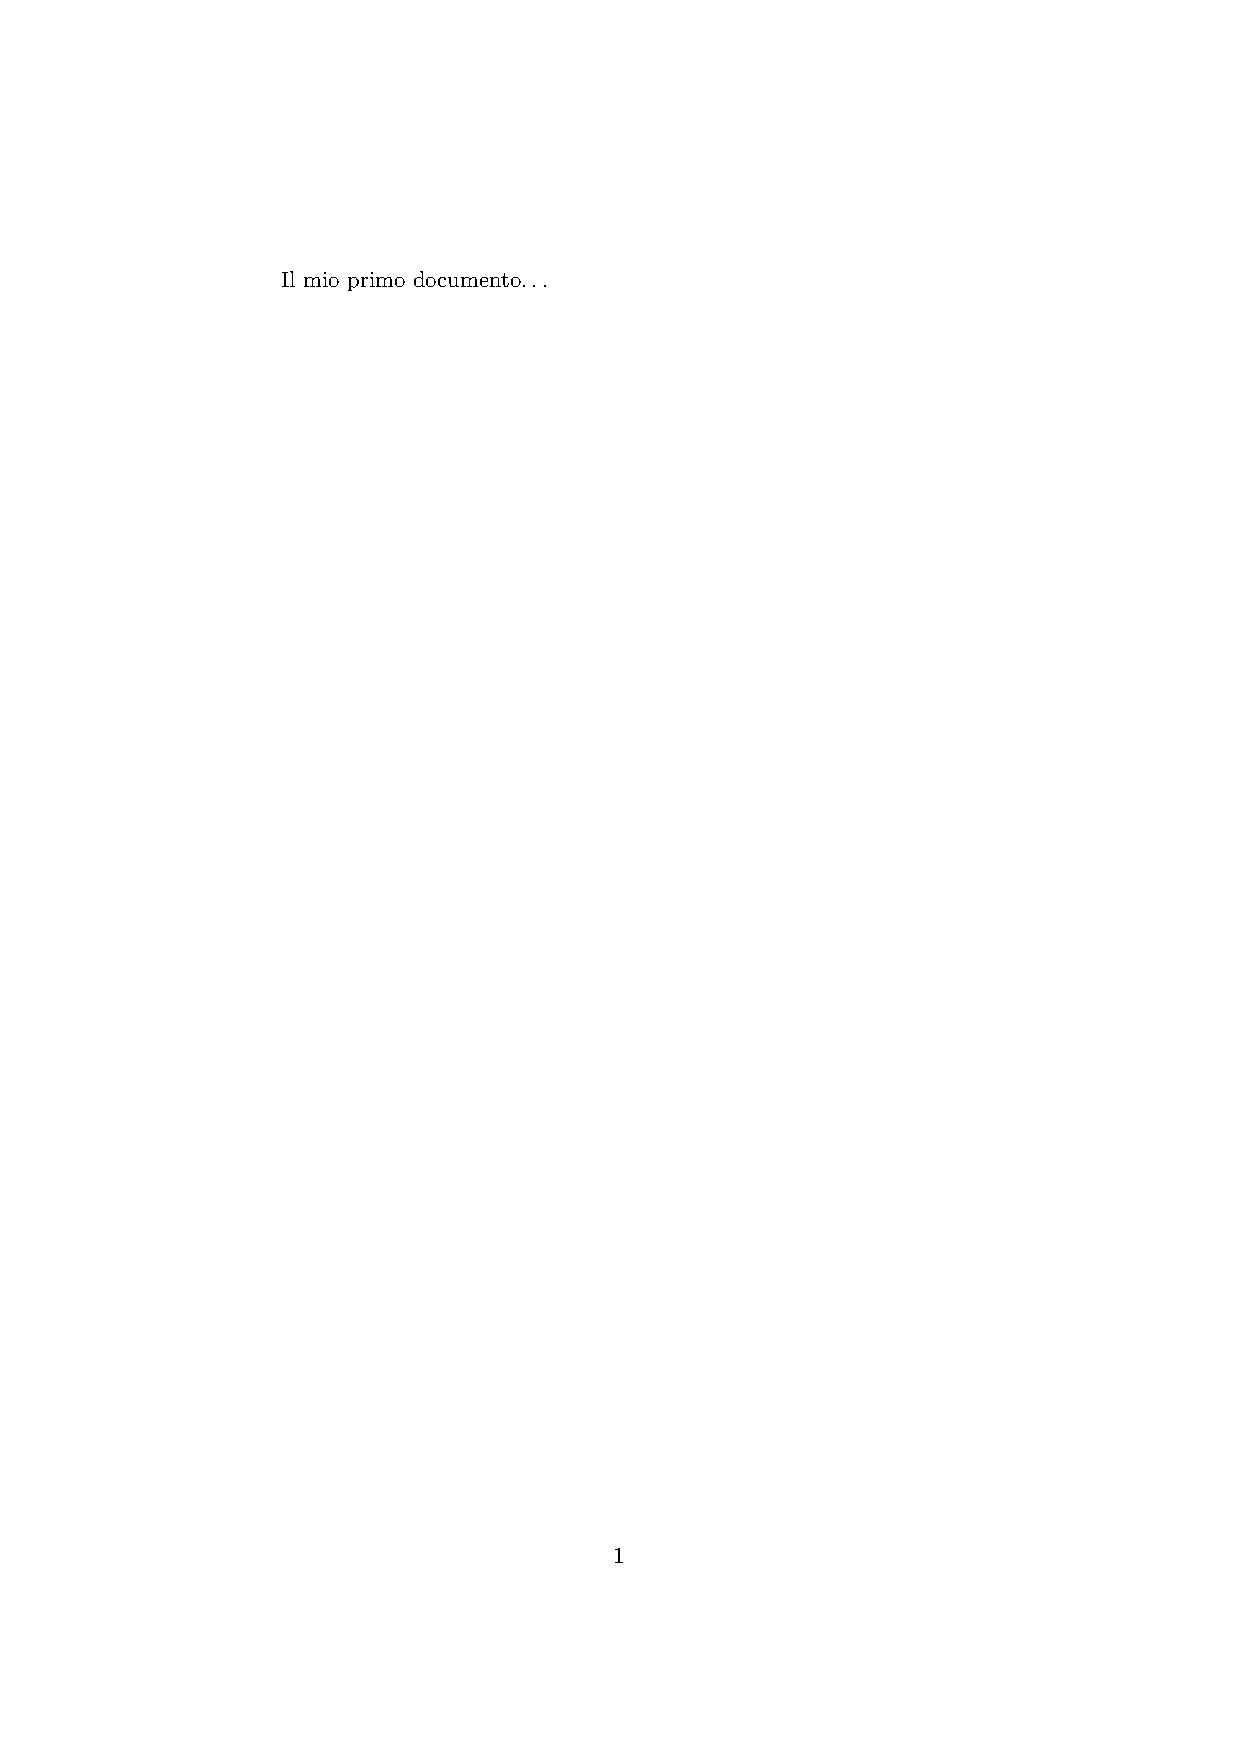
\includegraphics[width=14cm]{./ps_LaTeX/figure/documento1}}}
{Risultato della compilazione del documento \LaTeX\ riportato nel
paragrafo \ref{sec:Documento1}.}
{fig:Documento1}
Non \`e niente di esaltante, bisogna ammetterlo\ldots Ma prima di andare
avanti e familiarizzare con funzionalit\`a pi\`u potenti ed avanzate,
cerchiamo di capire il significato di ciascuna delle quattro righe del nostro
documento. Una per una.

\begin{verbatim}
\documentclass[11pt, a4paper]{article}
\end{verbatim}
Qui dichiariamo sostanzialmente il tipo di documento. Diciamo che si tratta di
un documento del tipo \emph{article}%
\footnote{
Esistono moltissimi tipi diversi di documenti predefiniti in \LaTeX\, tra cui
\emph{book}, \emph{report}, \emph{letter} e \emph{slides}; altri possono essere
aggiunti, anche se non si tratta esattamente della cosa pi\`u semplice del
mondo. Il tipo \emph{article} si presta piuttosto bene alla stesura di una
relazione di media lunghezza su una esperienza didattica ed \`e questo il
motivo per cui lo abbiamo scelto per i nostri esempi. 
}%
, che la dimensione dei caratteri del testo ordinario \`e $11$ punti%
\footnote{
Esistono anche le varianti 10 e 12 punti.
}%
, e che la dimensione della pagina \`e quella di un foglio A4%
\footnote{
Altri formati validi, solo per citarne un paio, sono \emph{a5paper}
e \emph{letterpaper}.
}
(che \`e la scelta tipica).

\begin{verbatim}
\begin{document}
\end{verbatim}
Segna l'inizio del documento vero e proprio. In generale questo comando separa
quello che \`e chiamato \emph{preambolo} (nel nostro caso \`e sostanzialmente
la linea precedente) dal \emph{corpo} vero e proprio del documento, che \`e
\emph{sempre} contenuto tra un comando di inizio ed un comando di fine
documento.

\begin{verbatim}
Il mio primo documento\ldots
\end{verbatim}
Si tratta del corpo del nostro documento, ed in effetti \`e la parte che
compare nella versione pronta per la stampa, come si pu\`o vedere in figura
\ref{fig:Documento1}.

\begin{verbatim}
\end{document}
\end{verbatim}
Questa linea chiude il documento ed \`e sempre richiesta alla fine di un
\emph{file} \LaTeX\ valido.

Nel prossimo paragrafo vedremo un esempio di documento pi\`u realistico e
cominceremo ad apprezzare alcune funzionalit\`a pi\`u utili ed avanzate.


\section{Un documento realistico}
\label{sec:Documento2}

Consideriamo attentamente il documento \LaTeX\ (valido) che segue\ldots

\begin{verbatim}
\documentclass[11pt, a4paper]{article}
\title{Il mio primo documento}
\author{Luca Baldini}
\date{20 Giugno 2006}

\begin{document}
\maketitle

\section{Introduzione}
Questo vuole essere un esempio di documento realistico, con lo scopo
di mostrare alcune tra le funzionali\`a di base di \LaTeX.

\section{Un nuovo capitolo}
Una prima cosa da notare \`e che, una volta dichiarate le sezioni del
documento, \LaTeX\ si occupa automaticamente della numerazione. Questo
pu\`o risultare estremamente utile nel caso in cui si voglia aggiungere
una nuova sezione in mezzo ad un documento in stato avanzato di stesura
(non \`e necessario rinumerare ci\`o che viene dopo, \LaTeX\ fa
tutto da solo). 

\subsection{Una sotto-sezione}
Come vedete esiste anche un livello pi\`u \emph{basso} di sezionamento
del documento.

\subsection{Ancora una sottosezione}
Anche a questo livello la numerazione \`e automatica. Questo consente
anche, in documenti pi\`u complessi, la generazione automatica dell'indice.

\section{Conclusioni}
Per il momento ci fermiamo qui, abbiamo abbastanza di cui discutere\ldots

\end{document}
\end{verbatim}

\noindent \ldots e vediamo come appare l'uscita del compilatore, pronta per
la stampa, che \`e riportata in figura \ref{fig:Documento2}.
\panelfig
{\framebox{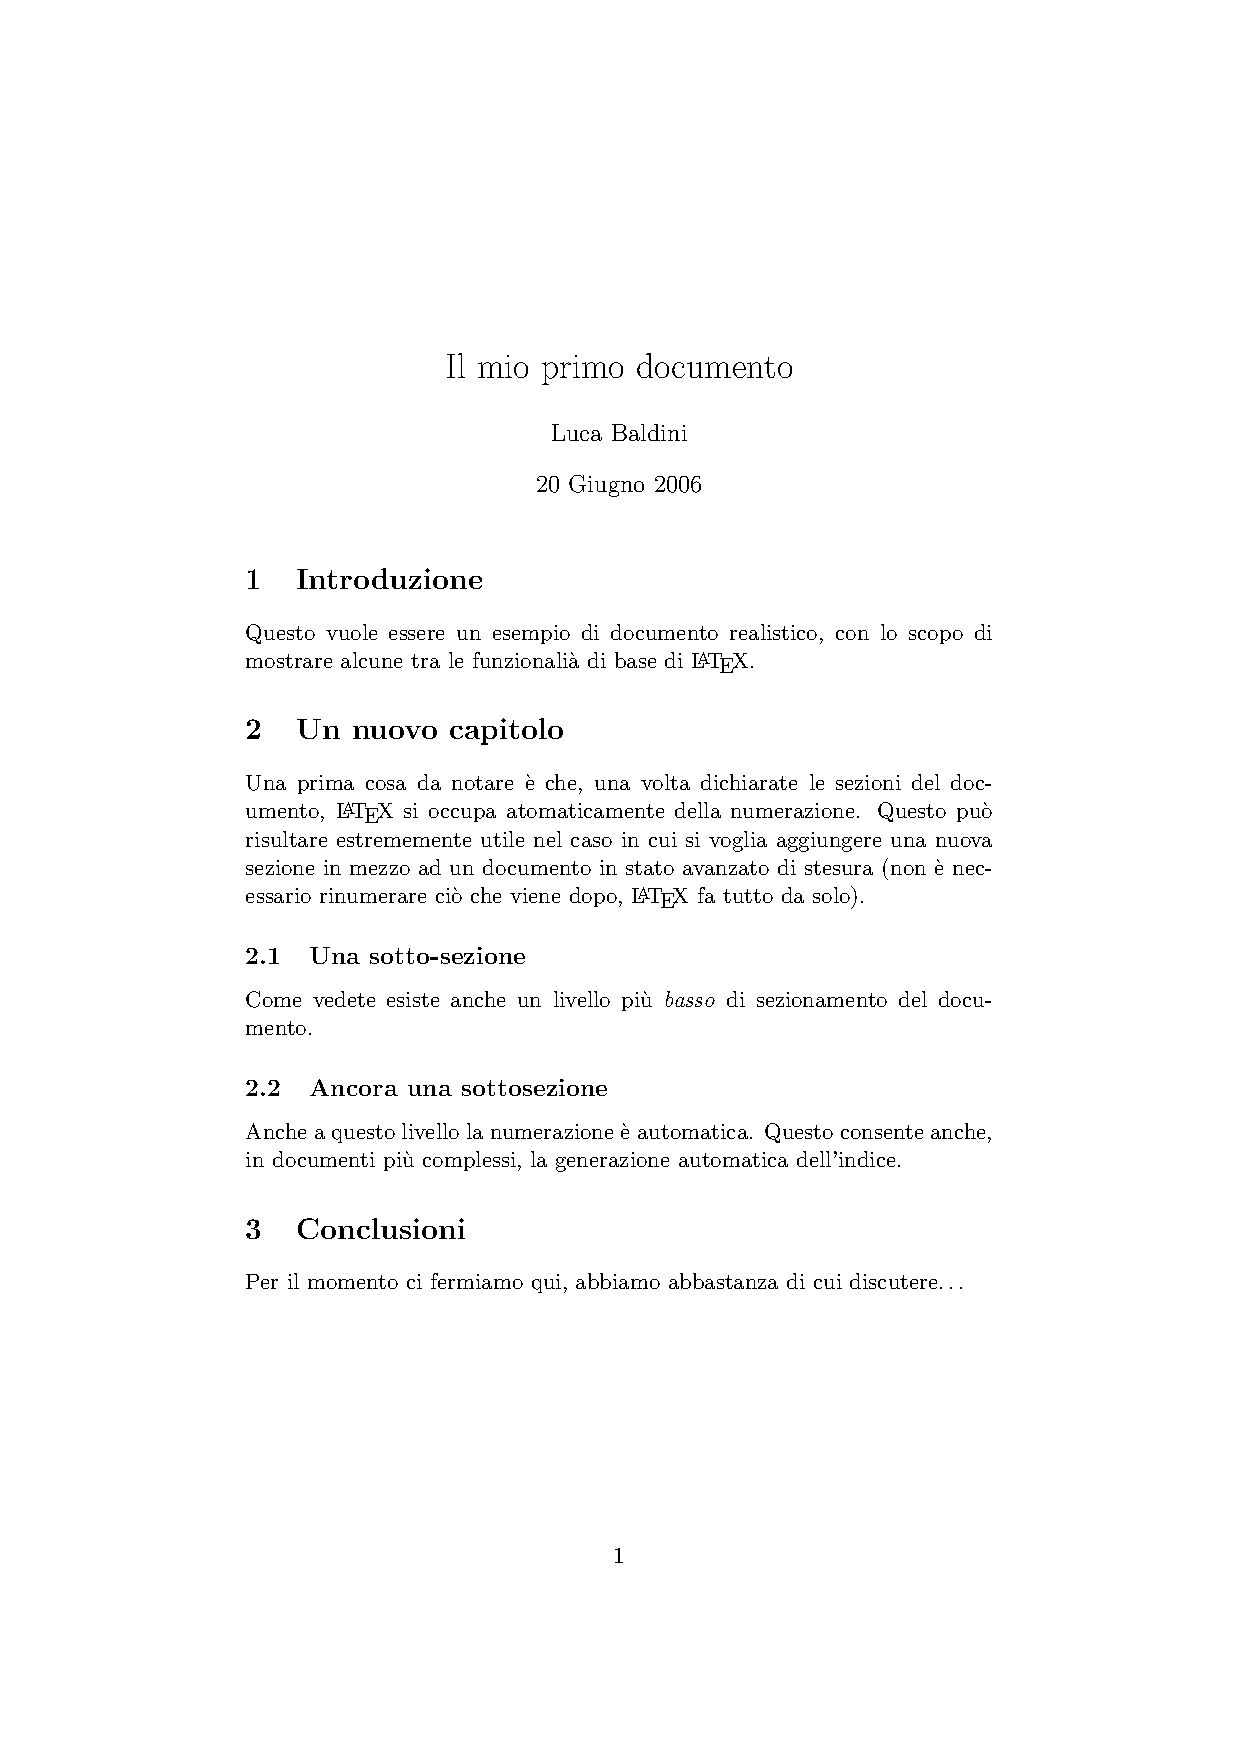
\includegraphics[width=14cm]{./ps_LaTeX/figure/documento2}}}
{Risultato della compilazione del documento \LaTeX\ riportato nel
paragrafo \ref{sec:Documento2}.}
{fig:Documento2}
Cominciamo con alcuni commenti di carattere generale per poi passare
all'analisi di alcuni tra i nuovi comandi che abbiamo appena incontrato.

Tutti i comandi \LaTeX\ cominciano con il carattere ``\verb|\|''
(\emph{backslash}). Alcuni di essi accettano (o richiedono, a seconda del
caso) \emph{opzioni} (che sono sempre contenute tra parentesi quadre) e
\emph{argomenti} (racchiusi tra parentesi graffe).
I comandi ed il testo sono, come \`e evidente, mischiati insieme all'interno
del documento. \`E importante notare come gli spazi multipli siano trattati
come  spazi singoli e come i ritorni a capo siano semplicemente ignorati,
se non che una linea vuota segna l'inizio di un nuovo paragrafo.
Esiste ovviamente un comando per andare a capo ed \`e ``\verb|\\|''
(doppio \emph{backslash}).

Tra i comandi rivestono particolare importanza quelli di sezionamento, che sono
utilizzati molto frequentemente. I documenti di tipo \emph{article} ammettono
i due comandi di sezionamento:
\begin{verbatim}
\section{}
\subsection{}
\end{verbatim}
che accettano come argomento il titolo della sezione o della sotto-sezione,
rispettivamente.

Una volta definito il tipo di documento, \LaTeX\ si occupa automaticamente sia
di numerare le sezioni e le sotto-sezioni che di fissare le dimensioni e
le altre caratteristiche dei caratteri per il testo ordinario e per i titoli.
Si tratta di un punto qualificante della filosofia di \LaTeX: il documento non
contiene, al suo interno, alcuna informazione riguardante la formattazione.
Ovviamente \`e possibile fare ogni genere di cambiamento, ma questo avviene
ordinariamente nel preambolo attraverso comandi specifici. Rimandiamo ai
riferimenti bibliografici per questi argomenti, che sono, in un certo senso,
pi\`u avanzati.

Veniamo adesso alla descrizione (sintetica, per necessit\`a) di alcuni dei
nuovi comandi che abbiamo introdotto.

\begin{verbatim}
\title{Il mio primo documento}
\author{Luca Baldini}
\date{20 Giugno 2006}
\end{verbatim}
Questo blocco definisce, come \`e naturale aspettarsi, il titolo, l'autore e
la data di composizione del documento, rispettivamente.
Se il comando date non viene dato esplicitamente, \LaTeX\ scrive
automaticamente la data del giorno, mutuata dal tempo di sistema del
calcolatore. Di \emph{default} questa data viene scritta in lingua inglese,
ma si pu\`o ovviare a questo inconveniente mettendo nel preambolo il comando
``\verb|\usepackage[italian]{babel}|''. Se non si vuole la data \`e
sufficiente scrivere ``\verb|\date{}|''.

Vale la pena notare che, di per s\'e,  questi comandi non hanno alcun effetto
(provare per credere!), a meno che non siano seguiti, nel corpo del documento,
dal comando:
\begin{verbatim}
\maketitle
\end{verbatim}

I pi\`u attenti avranno notato come sono state \emph{prodotte} le lettere
accentate. Ad esempio i due comandi ``\verb|\`e|'' e ``\verb|\'e|'' generano,
dopo la compilazione, i due caratteri ``\`e'' ed ``\'e'' (cogliamo l'occasione
per ricordare che la lingua Italiana possiede due accenti distinti: quello
grave e quello acuto).
Si tratta di un altro tratto distintivo della filosofia di \LaTeX, per cui si
tende a costruire esplicitamente gli oggetti complicati (ad esempio una
lettera accentata) a partire da oggetti pi\`u semplici (la lettera e
l'accento), anzich\'e avere un numero divergente di oggetti (e di tasti,
in questo caso\ldots) fin dall'inizio%
\footnote{
Ad essere onesti \LaTeX\ offre supporto completo, previa dichiarazione di un
apposito pacchetto nel preambolo, per la tastiera Italiana e, quindi, per le
ordinarie lettere accentate. Il lettore interessato pu\`o trovare le
informazioni relative nella documentazione specifica.
}%
.
Non serve aggiungere che il gioco funziona non solo con la a, ma con tutte le
vocali (ed anche con le consonanti, sebbene il risultato non sia in genere
particolarmente utile).


\section{Elenchi}

Molte delle esigenze pi\`u avanzate del semplice testo vengono gestite
in \LaTeX\ attraverso specifici \emph{ambienti} predefiniti.
Tecnicamente un ambiente \`e una porzione di documento inclusa tra un comando
``\verb|\begin{nome_ambiente}|'' ed un comando ``\verb|\end{nome_ambiente}|''.

Esistono \emph{ambienti}, ad esempio, per la creazione di elenchi puntati e
numerati. Le seguenti linee:
\begin{verbatim}
\begin{itemize}
\item{Punto primo.}
\item{Punto secondo.}
\end{itemize}
\end{verbatim}
producono, dopo la compilazione:
\begin{itemize}
\item{Punto primo.}
\item{Punto secondo.}
\end{itemize}
D'altra parte questo frammento:
\begin{verbatim}
\begin{enumerate}
\item{Punto primo.}
\item{Punto secondo.}
\end{enumerate}
\end{verbatim}
genera:
\begin{enumerate}
\item{Punto primo.}
\item{Punto secondo.}
\end{enumerate}


\section{Tabelle}

Le tabelle si costruiscono, secondo la filosofia di \LaTeX, a partire da
elementi \emph{semplici}: essenzialmente linee e caratteri come
mostrato nel frammento di codice che segue:
\begin{verbatim}
\begin{tabular}{cc}
\hline
Colonna 1 & Colonna 2 \\
\hline
\hline
a & b \\
c & d \\
\hline
\end{tabular}
\end{verbatim}
e che, compilato, genera:

\vspace{0.5 cm}
\begin{tabular}{cc}
\hline
Colonna 1 & Colonna 2 \\
\hline
\hline
a & b \\
c & d \\
\hline
\end{tabular}
\vspace{0.5 cm}

\noindent Analizziamo in dettaglio queste poche righe una alla volta. La prima:
\begin{verbatim}
\begin{tabular}{cc}
\end{verbatim}
\`e piuttosto densa di significato. Sostanzialmente segna l'inizio
dell'ambiente \cchar{tabular} e dichiara una tabella di due colonne.
Ognuna delle due \cchar{c} sta qui per \emph{center} e sta ad indicare
che il contenuto della colonna corrispondente sar\`a centrato.
Il lettore non sar\`a stupito di sentire che \`e possibile allineare
a destra o a sinistra il contenuto delle colonne usando \cchar{r}
(\emph{right}) o \cchar{l} (\emph{left}), rispettivamente%
\footnote{Per completezza ricordiamo che in \LaTeX\ \`e possibile utilizzare
il delimitatore \cchar{|} per separare le colonne di una tabella con linee
verticali---in questo caso particolare potremmo scrivere, ad esempio,
\cchar{|c|c|} anzich\'e \cchar{cc}. Tuttavia l'uso di separatori verticali
nelle tabelle non \`e considerata una buona pratica tipografica.}%
.

Le linee orizzontali debbono essere esplicitamente dichiarate tramite il
comando ``\verb|\hline|'' ed il contenuto vero e proprio della tabella \`e
strutturato come nella riga seguente:
\begin{verbatim}
a & b \\
\end{verbatim}
Il carattere \cchar{\&} serve da separatore tra celle contigue appartenenti
alla stessa linea, mentre il doppio \emph{backslash} (``\verb|\\|'') funge da
terminatore di linea.

Vale la pena, trovandoci in argomento, notare che con poche righe in pi\`u:
\begin{verbatim}
\begin{table}[!htb]
\begin{center}
\begin{tabular}{cc}
\hline
Colonna 1 & Colonna 2 \\
\hline
\hline
a & b \\
c & d \\
\hline
\end{tabular}
\caption{Questa \`e una tabella di esempio.}
\end{center}
\end{table}
\end{verbatim}
\`e possibile ottenere un risultato estremamente pi\`u appagante da un punto
di vista estetico (cfr. tabella~\ref{tabella_esempio}).
\begin{table}[htb!]
\begin{center}
\begin{tabular}{cc}
\hline
Colonna 1 & Colonna 2 \\
\hline
\hline
a & b \\
c & d \\
\hline
\end{tabular}
\caption{Questa \`e una tabella di esempio.}
\label{tabella_esempio}
\end{center}
\end{table}
Esaminiamo le differenze una per una. La pi\`u evidente \`e che adesso la
tabella \`e centrata. Questo si ottiene banalmente includendola all'interno dei
comandi:
\begin{verbatim}
\begin{center}
\end{center}
\end{verbatim}
I pi\`u attenti avranno anche notato che abbiamo introdotto un ulteriore nuovo
ambiente attraverso le due linee:
\begin{verbatim}
\begin{table}[!htb]
\end{table}
\end{verbatim}
Questo ha due (benefici) effetti distinti. Il primo \`e che diventa possibile
aggiungere una didascalia (automaticamente numerata) alla tabella attraverso
il comando:
\begin{verbatim}
\caption{}
\end{verbatim}
Il secondo (e pi\`u importante) \`e che la tabella diventa un oggetto
\emph{flottante}, cio\`e la sua posizione all'interno del documento pronto
per la stampa (dopo la compilazione) non \`e pi\`u fissata.
L'ambiente \cchar{table} \`e in effetti il primo esempio che incontriamo di
ambiente flottante; ne vedremo almeno un altro (\cchar{figure}) nel seguito.

Molti, all'inizio, si trovano in imbarazzo di fronte agli oggetti flottanti
ed hanno l'impressione di non riuscire a prendere il controllo sul
posizionamento di figure e tabelle. Si tratta effettivamente di un argomento
piuttosto complicato che non abbiamo il tempo di trattate approfonditamente
qui---rimandiamo il lettore alle indicazioni bibliografiche.
Ci limitiamo a notare che in generale l'inserimento di figure e tabelle in
posizioni \emph{fisse} rispetto al corpo del testo \`e considerata una pessima
pratica tipografica. In altre parole non \`e saggio pretendere di
posizionare una figura \emph{esattamente} di seguito ad una determinata linea
di testo; dopo l'impaginazione finale quella linea potrebbe essere tanto
vicina al margine inferiore della pagina da non lasciare fisicamente
abbastanza spazio. E di sicuro non \`e una cosa a cui si deve pensare
\emph{durante} la stesura di un documento---\`e un lavoro da tipografo, non
da scrittore.
Il consiglio, qui, \`e di rilassarsi e di lasciare a \LaTeX\ il lavoro
sporco; nella maggior parte dei casi sar\`a perfettamente in grado di
inserire gli oggetti flottanti nel modo pi\`u \emph{naturale} possibile
all'interno del testo. L'autore pu\`o aumentare la leggibilit\`a del
documento, come vedremo, aggiungendo riferimenti incrociati.

Adesso esaminiamo di nuovo la linea:
\begin{verbatim}
\begin{table}[!htb]
\end{verbatim}
e cerchiamo di capire il significato dell'opzione \cchar{!htb} che abbiamo
passato al comando. Le tre lettere \cchar{h} (\emph{here}),
\cchar{t} (\emph{top}) e \cchar{b} (\emph{bottom}),
in ordine, dicono a \LaTeX\ dov'\`e che vorremmo il nostro oggetto
flottante; in questo caso \LaTeX\ prover\`a ad inserirlo esattamente
dove esso \`e definito nel corpo del testo (\emph{here}) e, se questo
per qualche ragione non fosse possibile, lo inserir\`a all'inizio (\emph{top})
o alla fine (\emph{bottom}) della prima pagina successiva disponibile.
Il punto esclamativo (\cchar{!}), in un certo senso, rafforza l'opzione ed
\emph{obbliga} \LaTeX\ a mettere per un attimo da parte il proprio spiccato
senso estetico e ad assecondare la richiesta dell'autore, a meno che non
manchi fisicamente lo spazio per farlo.
L'opzione \cchar{!htb} dovrebbe essere sufficiente per la maggior parte
delle applicazioni non troppo avanzate---per quello che pu\`o contare tutte
le figure di queste dispense sono state inserite in questo modo.


\section{\LaTeX\ e la matematica}

Veniamo adesso ad uno dei motivi per cui \LaTeX\ ha riscosso tanto successo
all'interno della comunit\`a scientifica: l'estensivo supporto che fornisce
alla scrittura di simboli ed equazioni, che lo rende particolarmente indicato
per la scrittura di articoli scientifici%
\footnote{
In effetti \`e probabilmente sensato, di passaggio, ricordare che l'autore
originario di \TeX\, il \emph{motore tipografico} che sta alla base di \LaTeX\
\`e proprio un matematico, Donald E. Knuth}%
.

\LaTeX\ offre numerosi ambienti per la matematica; ne citeremo qui solamente
due: \cchar{math} ed \cchar{equation}. Il primo permette di inserire simboli
matematici all'interno del testo e si apre e chiude essenzialmente con un
simbolo \cchar{\$}. Ad esempio:
\begin{verbatim}
$\sigma_{x} = \sqrt{\sigma_{x}^{2}}$
\end{verbatim}
diviene, dopo la compilazione, $\sigma_{x} = \sqrt{\sigma_{x}^{2}}$.
Notiamo, per inciso, il comando ``\verb|\sqrt{}|'' che permette di inserire
radici quadrate di espressioni. Dovrebbe essere altres\`i chiaro
come inserire lettere greche e caratteri in apice e pedice.

L'ambiente equation permette di scrivere vere e proprie equazioni (numerate),
separate dal corpo del testo%
\footnote{
Potr\`a apparire curioso, ma non \`e permesso (provare per credere) lasciare
linee vuote all'interno dell'ambiente \emph{equation}.
}%
. Ad esempio:
\begin{verbatim}
\begin{equation}\label{osc_armonico}
m \frac{d^{2}x}{dt^{2}} = m \ddot x = -k x
\end{equation}
\end{verbatim}
diviene:
\begin{equation}\label{osc_armonico}
m \frac{d^{2}x}{dt^{2}} = m \ddot x = -k x
\end{equation}
Il lettore potr\`a essere incuriosito dal comando ``\verb|\label{}|'';
sostanzialmente esso permette di mettere un'etichetta in corrispondenza di un
oggetto%
\footnote{
In questo caso l'oggetto in questione \`e un'equazione, ma il tutto funziona
altrettanto bene con tabelle, figure, titoli di sezioni e paragrafi etc.
}%
, o in altre parole di assegnargli un nome comprensibile di modo che in
seguito, nel corpo del testo, ci si possa riferire ad esso in modo
univoco con l'apposito comando ``\verb|\ref{}|''.
Se, ad esempio, adesso scriviamo:
\begin{verbatim}
la (\ref{osc_armonico}) \`e l'equazione di moto di un oscillatore armonico.
\end{verbatim}
dopo la compilazione ci\`o che otteniamo \`e:
la (\ref{osc_armonico}) \`e l'equazione di moto di un oscillatore armonico.
I due comandi ``\verb|\label{}|'' e ``\verb|\ref{}|'' sono incredibilmente
utili.
Pensate a quanti riferimenti numerati ad ogni tipo di oggetto vi sono in queste
dispense\ldots senza un meccanismo del genere tenere oggetti e riferimenti
sincronizzati sarebbe stato letteralmente un inferno!

\caution{Gli spazi all'interno degli ambienti matematici vengono ignorati.
\LaTeX\ ha un suo algoritmo piuttosto sofisticato per determinare
automaticamente le spaziature necessarie tra i vari oggetti in modalit\`a
matematica.}

Chiudiamo il paragrafo con un'ultima equazione, che mostra un certo numero
di comandi utili:
\begin{verbatim}
\begin{equation}
\left( \int_{-\infty}^{\infty} e^{-x^{2}} dx \right)^{2} =
\sum_{n=0}^{\infty}\frac{(-1)^{n}}{2n + 1} =
\prod_{n=1}^{\infty} \left( \frac{n + 1}{n} \right)^{(-1)^{n-1}} =
\pi
\end{equation}
\end{verbatim}
che appare come:
\begin{equation}
\left( \int_{-\infty}^{\infty} e^{-x^{2}} dx \right)^{2} =
\sum_{n=0}^{\infty}\frac{(-1)^{n}}{2n + 1} =
\prod_{n=1}^{\infty} \left( \frac{n + 1}{n} \right)^{(-1)^{n-1}} =
\pi
\end{equation}
Rimandiamo il lettore alla documentazione specifica per una trattazione
esaustiva delle funzionalit\`a offerte da \LaTeX\ in modalit\`a matematica.


\section{Inserire le figure}

Eccoci all'ultimo argomento di questa breve rassegna sulle funzionalit\`a di
base di \LaTeX: l'inserimento delle figure.
\begin{figure}[h!]
\begin{center}
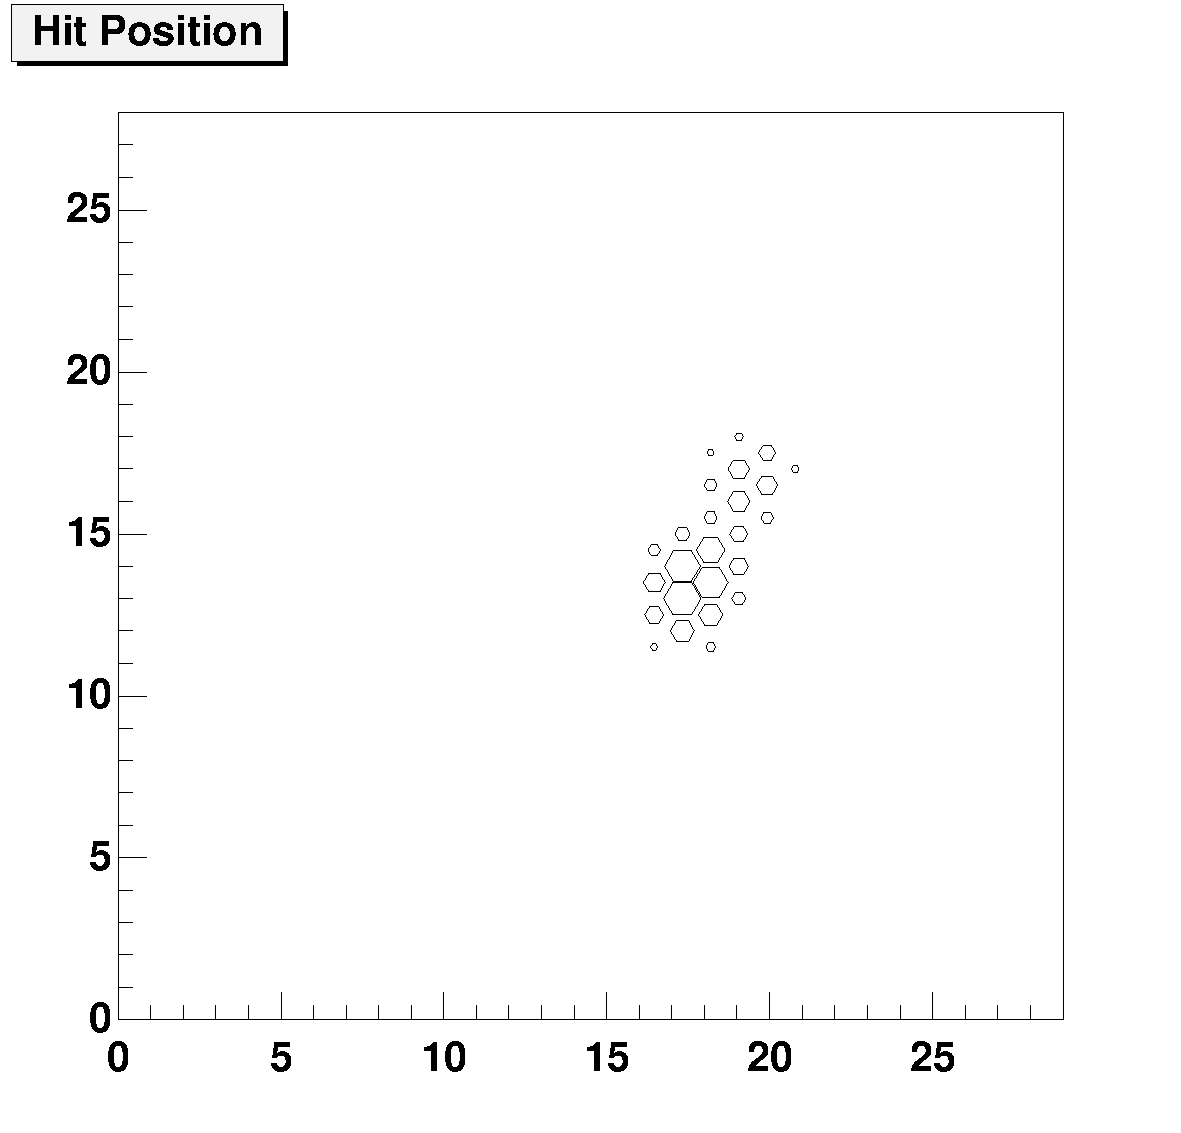
\includegraphics[width=5.8cm]{./ps_LaTeX/figure/test.pdf}
\end{center}
\caption{Questa \`e una figura di esempio.}
\label{figura_di_esempio}
\end{figure}
La prima cosa che dobbiamo fare \`e includere un pacchetto specifico, e
questo si fa inserendo all'interno del preambolo il comando:
\begin{verbatim}
\usepackage[dvips]{graphicx}
\end{verbatim}
Fatto questo, grafici ed immagini in formato eps%
\footnote{
Il formato eps (\emph{Encapsulated PostScript}) \`e piuttosto usato,
specialmente nella comunit\`a scientifica, per la creazioni di grafici,
schemi sintetici ed oggetti di grafica vettoriale in generale (sostanzialmente
tutto ci\`o che \`e costituito da linee, punti e lettere).
Vedremo nel prossimo capitolo come creare grafici eps utilizzando il programma
di analisi dati \gnuplot.
}
possono essere inseriti con poche linee (il risultato della compilazione
appare in figura~\ref{figura_di_esempio}):
\begin{verbatim}
\begin{figure}[!htb]
\begin{center}
\includegraphics[width=5.8cm]{./ps_LaTeX/figure/Test.eps}
\end{center}
\caption{Questa \`e una figura di esempio.}
\label{figura_di_esempio}
\end{figure}
\end{verbatim}

Sostanzialmente non vi \`e niente di nuovo se non l'ambiente (flottante)
\cchar{figure}, per cui vale quanto detto a proposito di \cchar{table},
ed il comando:
\begin{verbatim}
\includegraphics[width=8cm]{./ps_LaTeX/figure/Test.eps}
\end{verbatim}
cui \`e passato il nome del \emph{file} eps come argomento e la larghezza
con cui l'immagine in esso contenuta deve apparire nel documento.
Notiamo, per inciso, che ``\verb|\includegraphics|'' \`e il comando che
richiede il pacchetto \cchar{graphicx}.

Si possono ovviamente anche inserire figure in formato diverso dal
postscript (ad esempio jpg, png etc.). L'unica differenza \`e che in questo
caso bisogna specificare esplicitamente le dimensioni dell'immagine%
\footnote{
Tecnicamente questo \`e conseguenza del fatto che il formato eps, a differenza
degli altri, contiene al suo interno la definizione della cosiddetta
\emph{bounding box}.
}
tra le opzioni di ``\verb|\includegraphics|''.
Se, per esempio, supponiamo di voler inserire una figura in formato jpg
di $800\times 600$ pixel, dovremo scrivere qualcosa del tipo:
\begin{verbatim}
\includegraphics[width=8cm, bb=0 0 800 600]{./Figura.jpg}
\end{verbatim}
in cui il frammento \cchar{bb=0 0 800 600}
fornisce appunto la dimensione della \emph{cornice} che racchiude l'immagine
(cio\`e della \emph{bounding box}), nella forma delle coordinate (espresse in
pixel) degli angoli in alto a sinistra (\cchar{0 0}) ed in basso a destra
(\cchar{800 600}) della cornice stessa.
.

\chapter{Visualizzare ed analizzare dati: \gnuplot}
\label{chap:gnuplot}
\mt


Inutile dire che di programmi per la visualizzazione e l'analisi
di dati scientifici ce sono per tutti i gusti. Nell'imbarazzo della scelta
abbiamo optato per \gnuplot, guidati da una serie di considerazioni che vale
la pena di esporre brevemente.

Per prima cosa \gnuplot\ \`e \emph{freeware}, \emph{open source} ed \`e
sviluppato ed utilizzato da una comunit\`a decisamente ampia, il che \`e
garanzia di affidabilit\`a e supporto estensivo per l'utente, a partire
dalla documentazione.

Inoltre \gnuplot\ \`e, se paragonato alla maggior parte dei \emph{prodotti}
concorrenti, sorprendentemente \emph{semplice}, nel senso che tipicamente
permette di eseguire con poca difficolt\`a tutte quelle operazioni a cui il
fisico si trova spesso di fronte (visualizzazione di dati e funzioni, fit,
etc.), per lo meno nelle analisi non troppo sofisticate.

Terzo ed ultimo (anche se non in importanza) punto: \gnuplot\ si gestisce
completamente da linea di comando attraverso un \emph{macrolinguaggio} nativo
e \emph{non} attraverso un'interfaccia grafica.
Sebbene questo possa sembrare a prima vista uno svantaggio (retaggio di un
tempo ormai andato in cui i calcolatori erano dei deprimenti schermi neri con
su qualche scritta incomprensibile) avremo occasione di vedere nel seguito
che si tratta invece di una notevole facilitazione quando si voglia
eseguire molte volte la stessa sequenza (anche complessa) di operazioni.


\section{Lanciare \gnuplot}

Se stiamo lavorando sotto \linux%
\footnote{
Sotto \windows\ \gnuplot\ \`e disponibile sotto forma di eseguibile e
tipicamente si lancia con un doppio click di mouse sull'eseguibile stesso.
Se le variabili di ambiente sono impostate correttamente (ed in particolare
il percorso completo all'eseguibile di \gnuplot\ \`e contenuto nella variabile
d'ambiente PATH), allora il programma si pu\`o anche lanciare dal prompt di
\dos\ e l'uso diventa essenzialmente identico a quello sotto \linux.
Nel seguito cercheremo via via di mettere in evidenza le differenze di
impiego tra i due sistemi operativi.
}%
, digitare il comando \cchar{gnuplot} dovrebbe essere sufficiente
per avere indietro una schermata \emph{simile} a questa:
\begin{verbatim}
>gnuplot

        G N U P L O T
        Version 4.0 patchlevel 0
        last modified Thu Apr 15 14:44:22 CEST 2004
        System: Linux 32 bit

        Copyright (C) 1986 - 1993, 1998, 2004
        Thomas Williams, Colin Kelley and many others

        This is gnuplot version 4.0.  Please refer to the documentation
        for command syntax changes.  The old syntax will be accepted
        throughout the 4.0 series, but all save files use the new syntax.

        Type `help` to access the on-line reference manual.
        The gnuplot FAQ is available from
                http://www.gnuplot.info/faq/

        Send comments and requests for help to
                <gnuplot-info@lists.sourceforge.net>
        Send bugs, suggestions and mods to
                <gnuplot-bugs@lists.sourceforge.net>


Terminal type set to 'x11'
gnuplot>
\end{verbatim}
Se ci\`o non accade vi \`e una probabilit\`a prossima all'unit\`a che il
programma non sia correttamente installato (o non sia installato affatto);
in questo caso porre rimedio all'inconveniente \`e facilissimo,
essendo \gnuplot\ incluso praticamente in tutte le distribuzioni \linux:
sar\`a sufficiente andare a ripescare i cd da cui si \`e installato il sistema
operativo.

Supponiamo dunque di aver eseguito con successo il nostro comando.
L'ultima linea
sullo schermo:
\begin{verbatim}
gnuplot>
\end{verbatim}
ci dice che ci troviamo all'interno della \emph{shell} di \gnuplot\ e che il
programma \`e pronto in attesa di comandi.
Se, come ci viene suggerito nella schermata iniziale, digitiamo il comando%
\footnote{
Per dovere di chiarezza notiamo esplicitamente, anche se non dovrebbe
essercene stretto bisogno, che, qui ed in tutto il seguito del capitolo,
il comando propriamente detto \`e tutto e solo ci\`o che segue
\cchar{gnuplot>} (che serve semplicemente ad indicare che, in un determinato
istante, ci troviamo entro la \emph{shell} di \gnuplot).
In questo caso particolare, dunque, l'utente digiter\`a fisicamente
\cchar{help} e non \cchar{gnuplot> help}. 
}%
:
\begin{verbatim}
gnuplot> help
\end{verbatim}
questo dovrebbe essere sufficiente per visualizzare l'aiuto interattivo,
che \`e sempre un buon punto di partenza.


\section{Due cose semplici (ma utili)\ldots}

Supponiamo di voler disegnare grafico della funzione:
\begin{equation}\label{eq:FunzioneGnuplot}
f(x) = \frac{\sin x}{x}
\end{equation}
Ebbene: in \gnuplot\ \`e sufficiente il singolo comando:
\begin{verbatim}
gnuplot> plot sin(x)/x
\end{verbatim}
per ottenere qualcosa di non troppo lontano da ci\`o che \`e mostrato in figura
\ref{fig:FunzioneGnuplot}:
\panelfig
{% GNUPLOT: LaTeX picture with Postscript
\begingroup
\footnotesize
  \makeatletter
  \providecommand\color[2][]{%
    \GenericError{(gnuplot) \space\space\space\@spaces}{%
      Package color not loaded in conjunction with
      terminal option `colourtext'%
    }{See the gnuplot documentation for explanation.%
    }{Either use 'blacktext' in gnuplot or load the package
      color.sty in LaTeX.}%
    \renewcommand\color[2][]{}%
  }%
  \providecommand\includegraphics[2][]{%
    \GenericError{(gnuplot) \space\space\space\@spaces}{%
      Package graphicx or graphics not loaded%
    }{See the gnuplot documentation for explanation.%
    }{The gnuplot epslatex terminal needs graphicx.sty or graphics.sty.}%
    \renewcommand\includegraphics[2][]{}%
  }%
  \providecommand\rotatebox[2]{#2}%
  \@ifundefined{ifGPcolor}{%
    \newif\ifGPcolor
    \GPcolorfalse
  }{}%
  \@ifundefined{ifGPblacktext}{%
    \newif\ifGPblacktext
    \GPblacktexttrue
  }{}%
  % define a \g@addto@macro without @ in the name:
  \let\gplgaddtomacro\g@addto@macro
  % define empty templates for all commands taking text:
  \gdef\gplbacktext{}%
  \gdef\gplfronttext{}%
  \makeatother
  \ifGPblacktext
    % no textcolor at all
    \def\colorrgb#1{}%
    \def\colorgray#1{}%
  \else
    % gray or color?
    \ifGPcolor
      \def\colorrgb#1{\color[rgb]{#1}}%
      \def\colorgray#1{\color[gray]{#1}}%
      \expandafter\def\csname LTw\endcsname{\color{white}}%
      \expandafter\def\csname LTb\endcsname{\color{black}}%
      \expandafter\def\csname LTa\endcsname{\color{black}}%
      \expandafter\def\csname LT0\endcsname{\color[rgb]{1,0,0}}%
      \expandafter\def\csname LT1\endcsname{\color[rgb]{0,1,0}}%
      \expandafter\def\csname LT2\endcsname{\color[rgb]{0,0,1}}%
      \expandafter\def\csname LT3\endcsname{\color[rgb]{1,0,1}}%
      \expandafter\def\csname LT4\endcsname{\color[rgb]{0,1,1}}%
      \expandafter\def\csname LT5\endcsname{\color[rgb]{1,1,0}}%
      \expandafter\def\csname LT6\endcsname{\color[rgb]{0,0,0}}%
      \expandafter\def\csname LT7\endcsname{\color[rgb]{1,0.3,0}}%
      \expandafter\def\csname LT8\endcsname{\color[rgb]{0.5,0.5,0.5}}%
    \else
      % gray
      \def\colorrgb#1{\color{black}}%
      \def\colorgray#1{\color[gray]{#1}}%
      \expandafter\def\csname LTw\endcsname{\color{white}}%
      \expandafter\def\csname LTb\endcsname{\color{black}}%
      \expandafter\def\csname LTa\endcsname{\color{black}}%
      \expandafter\def\csname LT0\endcsname{\color{black}}%
      \expandafter\def\csname LT1\endcsname{\color{black}}%
      \expandafter\def\csname LT2\endcsname{\color{black}}%
      \expandafter\def\csname LT3\endcsname{\color{black}}%
      \expandafter\def\csname LT4\endcsname{\color{black}}%
      \expandafter\def\csname LT5\endcsname{\color{black}}%
      \expandafter\def\csname LT6\endcsname{\color{black}}%
      \expandafter\def\csname LT7\endcsname{\color{black}}%
      \expandafter\def\csname LT8\endcsname{\color{black}}%
    \fi
  \fi
  \setlength{\unitlength}{0.0500bp}%
  \begin{picture}(7560.00,5040.00)%
    \gplgaddtomacro\gplbacktext{%
      \csname LTb\endcsname%
      \put(770,440){\makebox(0,0)[r]{\strut{}-0.4}}%
      \put(770,1059){\makebox(0,0)[r]{\strut{}-0.2}}%
      \put(770,1679){\makebox(0,0)[r]{\strut{} 0}}%
      \put(770,2298){\makebox(0,0)[r]{\strut{} 0.2}}%
      \put(770,2918){\makebox(0,0)[r]{\strut{} 0.4}}%
      \put(770,3537){\makebox(0,0)[r]{\strut{} 0.6}}%
      \put(770,4157){\makebox(0,0)[r]{\strut{} 0.8}}%
      \put(770,4776){\makebox(0,0)[r]{\strut{} 1}}%
      \put(902,220){\makebox(0,0){\strut{}-10}}%
      \put(2473,220){\makebox(0,0){\strut{}-5}}%
      \put(4044,220){\makebox(0,0){\strut{} 0}}%
      \put(5615,220){\makebox(0,0){\strut{} 5}}%
      \put(7186,220){\makebox(0,0){\strut{} 10}}%
    }%
    \gplgaddtomacro\gplfronttext{%
      \csname LTb\endcsname%
      \put(6199,4603){\makebox(0,0)[r]{\strut{}sin(x)/x}}%
    }%
    \gplbacktext
    \put(0,0){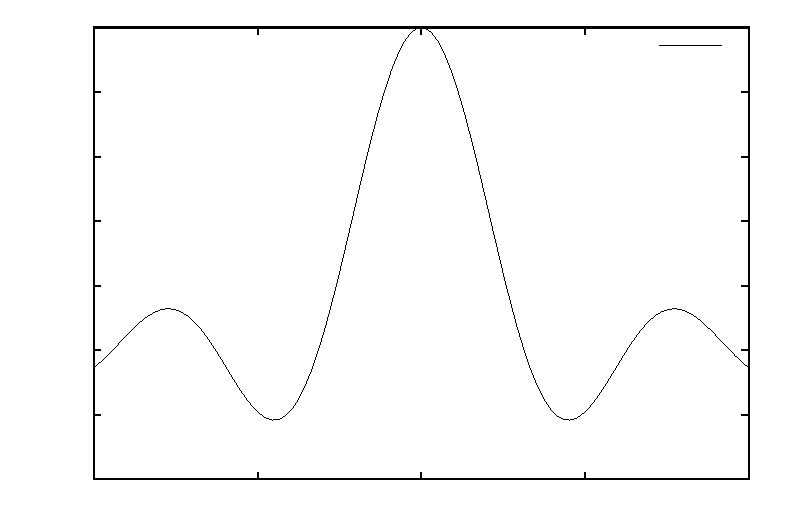
\includegraphics{function_small}}%
    \gplfronttext
  \end{picture}%
\endgroup
}
{Grafico della funzione (\ref{eq:FunzioneGnuplot}), prodotto
da \gnuplot\ con il semplice comando \cchar{plot sin(x)/x}.}
{fig:FunzioneGnuplot}

\noindent Teniamo a mente il comando \cchar{plot}, che abbiamo appena
utilizzato, perch\'e si tratta di uno dei comandi fondamentali e lo
incontreremo ancora sovente, nel seguito.

Trovandoci a parlare di funzioni, notiamo subito come \gnuplot\
supporti in modo estensivo essenzialmente tutte le funzioni con cui si ha a
che fare di solito nell'analisi di dati scientifici (queste includono, ma non
sono limitate a, funzioni trigonometriche, esponenziali e logaritmi).
Se siete incerti su come si possa scrivere il nome di una funzione in modo
che \gnuplot\ \emph{capisca} che cosa volete dire, provate semplicemente a
digitare:
\begin{verbatim}
gnuplot> help functions
\end{verbatim}
ed otterrete tutte le informazioni di cui avete bisogno.
Notiamo anche come le funzioni possano essere poi \emph{combinate}
ulteriormente tra di loro con gli usuali operatori aritmetici che si trovano
elencati in tabella
\ref{tab:OperatoriGnuplot}.

\begin{table}[htbp]
\stdtable{2}%
{Operatore           & Simbolo}%
{Addizione           & \texttt{+}\\
Sottrazione          & \texttt{-}\\
Moltiplicazione      & \texttt{*}\\
Divisione            & \texttt{/}\\
Elevamento a potenza & \texttt{**}\\
}
\caption{Associazione tra gli operatori aritmetici di base ed il simbolo
corrispondente all'interno della \emph{shell} di \gnuplot.}
\label{tab:OperatoriGnuplot}
\end{table}

Spulciando tra le funzioni disponibili all'interno di \gnuplot\ troviamo
anche, come era logico aspettarsi, la \emph{error function} che abbiamo
introdotto a proposito della distribuzione di Gauss e che si trova descritta
in dettaglio in appendice \ref{app:Erf} e tabulata nelle appendici
\ref{app:Erf1} e \ref{app:Erf2}.
In effetti possiamo leggere direttamente dalle tavole (cfr. \ref{app:Erf1}):
$$
\erf(1) = 0.3413
$$
Proviamo allora ad ottenere lo stesso risultato utilizzando \gnuplot; per far
questo ci servir\`a, come vedremo, il comando \cchar{print}, che
sostanzialmente consente di stampare sullo schermo%
\footnote{
Ad essere rigorosi questo non \`e necessariamente vero. Volendo, l'uscita del
comando print pu\`o essere rediretta su un \emph{file} attraverso l'apposito
comando \cchar{set print}.
}
il valore di un'espressione, passata come argomento. Digitiamo:
\begin{verbatim}
gnuplot> print erf(1)
0.842700790029219
\end{verbatim}
Vi \`e chiaramente qualcosa che non va, perch\'e il numero che otteniamo non
\`e corretto. Ma se leggiamo attentamente il contenuto dell'appendice
\ref{app:Erf}, vi troviamo un esplicito riferimento al fatto che ci sono due
definizioni differenti della \emph{error function}, $\erf(x)$ ed $\Erf(x)$,
legate dalla relazione:
$$
\erf(x) = \frac{1}{2} \Erf \left( \frac{x}{\sqrt{2}} \right)
$$
Nelle tavole numeriche noi utilizziamo la prima, ma potrebbe darsi che
\gnuplot\ usi l'altra. Proviamo allora a digitare:
\begin{verbatim}
gnuplot> print 0.5*erf(1/sqrt(2))
0.341344745680573
\end{verbatim}
Questa volta abbiamo il risultato corretto, il che conferma la nostra ipotesi.
Notiamo per inciso che, sebbene non costituisca il modo pi\`u efficiente,
il comando \cchar{print} permette, in linea di principio, di rigenerare le
tavole numeriche riportate nelle sopracitate appendici.
Pi\`u semplicemente, esso permette di evitare l'interpolazione tra valori
tabulati, ogni qual volta si abbia un calcolatore a disposizione.


\section{\ldots e due cose meno ovvie}

Vi sono situazioni in cui il calcolatore sembra fornire all'utente dei
risultati inaspettati, apparentemente errati, o addirittura assurdi.
Lo scopo dichiarato di questo paragrafo \`e di mostrare come, nella stragrande
maggioranza di questi casi, non sia il computer a sbagliare; pi\`u
semplicemente l'utilizzatore ha posto al computer una domanda che \`e
effettivamente \emph{diversa} da quella che egli stesso, in buona fede,
credeva aver posto.
Si pu\`o dire, a buon diritto, che in questa difficolt\`a di comunicazione
tra utente e calcolatore risieda l'origine di un gran parte degli errori di
programmazione. Che \`e come dire che, una volta pensata una \emph{domanda}
che si vuol porre al calcolatore, il punto fondamentale \`e formularla in
modo corretto nel linguaggio del calcolatore stesso.

Supponiamo dunque di voler disegnare il grafico della funzione
(\ref{eq:FunzioneGnuplot}) in un intervallo specifico della variabile
indipendente $x$. Per fissare li idee, supponiamo che questo intervallo
sia $\cinterval{-170}{170}$.
Vi \`e un comando specifico, \cchar{set xrange}, per fissare i limiti di
variabilit\`a della $x$, per cui proveremo a scrivere:
\begin{verbatim}
gnuplot> set xrange [-170:170]
gnuplot> plot sin(x)/x
\end{verbatim}
Il risultato, che \`e mostrato in figura \ref{fig:FunzioneGnuplotLarga},
non pu\`o non destare perplessit\`a.
\panelfig
{% GNUPLOT: LaTeX picture with Postscript
\begingroup
\footnotesize
  \makeatletter
  \providecommand\color[2][]{%
    \GenericError{(gnuplot) \space\space\space\@spaces}{%
      Package color not loaded in conjunction with
      terminal option `colourtext'%
    }{See the gnuplot documentation for explanation.%
    }{Either use 'blacktext' in gnuplot or load the package
      color.sty in LaTeX.}%
    \renewcommand\color[2][]{}%
  }%
  \providecommand\includegraphics[2][]{%
    \GenericError{(gnuplot) \space\space\space\@spaces}{%
      Package graphicx or graphics not loaded%
    }{See the gnuplot documentation for explanation.%
    }{The gnuplot epslatex terminal needs graphicx.sty or graphics.sty.}%
    \renewcommand\includegraphics[2][]{}%
  }%
  \providecommand\rotatebox[2]{#2}%
  \@ifundefined{ifGPcolor}{%
    \newif\ifGPcolor
    \GPcolorfalse
  }{}%
  \@ifundefined{ifGPblacktext}{%
    \newif\ifGPblacktext
    \GPblacktexttrue
  }{}%
  % define a \g@addto@macro without @ in the name:
  \let\gplgaddtomacro\g@addto@macro
  % define empty templates for all commands taking text:
  \gdef\gplbacktext{}%
  \gdef\gplfronttext{}%
  \makeatother
  \ifGPblacktext
    % no textcolor at all
    \def\colorrgb#1{}%
    \def\colorgray#1{}%
  \else
    % gray or color?
    \ifGPcolor
      \def\colorrgb#1{\color[rgb]{#1}}%
      \def\colorgray#1{\color[gray]{#1}}%
      \expandafter\def\csname LTw\endcsname{\color{white}}%
      \expandafter\def\csname LTb\endcsname{\color{black}}%
      \expandafter\def\csname LTa\endcsname{\color{black}}%
      \expandafter\def\csname LT0\endcsname{\color[rgb]{1,0,0}}%
      \expandafter\def\csname LT1\endcsname{\color[rgb]{0,1,0}}%
      \expandafter\def\csname LT2\endcsname{\color[rgb]{0,0,1}}%
      \expandafter\def\csname LT3\endcsname{\color[rgb]{1,0,1}}%
      \expandafter\def\csname LT4\endcsname{\color[rgb]{0,1,1}}%
      \expandafter\def\csname LT5\endcsname{\color[rgb]{1,1,0}}%
      \expandafter\def\csname LT6\endcsname{\color[rgb]{0,0,0}}%
      \expandafter\def\csname LT7\endcsname{\color[rgb]{1,0.3,0}}%
      \expandafter\def\csname LT8\endcsname{\color[rgb]{0.5,0.5,0.5}}%
    \else
      % gray
      \def\colorrgb#1{\color{black}}%
      \def\colorgray#1{\color[gray]{#1}}%
      \expandafter\def\csname LTw\endcsname{\color{white}}%
      \expandafter\def\csname LTb\endcsname{\color{black}}%
      \expandafter\def\csname LTa\endcsname{\color{black}}%
      \expandafter\def\csname LT0\endcsname{\color{black}}%
      \expandafter\def\csname LT1\endcsname{\color{black}}%
      \expandafter\def\csname LT2\endcsname{\color{black}}%
      \expandafter\def\csname LT3\endcsname{\color{black}}%
      \expandafter\def\csname LT4\endcsname{\color{black}}%
      \expandafter\def\csname LT5\endcsname{\color{black}}%
      \expandafter\def\csname LT6\endcsname{\color{black}}%
      \expandafter\def\csname LT7\endcsname{\color{black}}%
      \expandafter\def\csname LT8\endcsname{\color{black}}%
    \fi
  \fi
  \setlength{\unitlength}{0.0500bp}%
  \begin{picture}(7560.00,5040.00)%
    \gplgaddtomacro\gplbacktext{%
      \csname LTb\endcsname%
      \put(770,440){\makebox(0,0)[r]{\strut{}-0.2}}%
      \put(770,982){\makebox(0,0)[r]{\strut{}-0.1}}%
      \put(770,1524){\makebox(0,0)[r]{\strut{} 0}}%
      \put(770,2066){\makebox(0,0)[r]{\strut{} 0.1}}%
      \put(770,2608){\makebox(0,0)[r]{\strut{} 0.2}}%
      \put(770,3150){\makebox(0,0)[r]{\strut{} 0.3}}%
      \put(770,3692){\makebox(0,0)[r]{\strut{} 0.4}}%
      \put(770,4234){\makebox(0,0)[r]{\strut{} 0.5}}%
      \put(770,4776){\makebox(0,0)[r]{\strut{} 0.6}}%
      \put(1272,220){\makebox(0,0){\strut{}-150}}%
      \put(2196,220){\makebox(0,0){\strut{}-100}}%
      \put(3120,220){\makebox(0,0){\strut{}-50}}%
      \put(4044,220){\makebox(0,0){\strut{} 0}}%
      \put(4968,220){\makebox(0,0){\strut{} 50}}%
      \put(5892,220){\makebox(0,0){\strut{} 100}}%
      \put(6816,220){\makebox(0,0){\strut{} 150}}%
    }%
    \gplgaddtomacro\gplfronttext{%
      \csname LTb\endcsname%
      \put(6199,4603){\makebox(0,0)[r]{\strut{}sin(x)/x}}%
    }%
    \gplbacktext
    \put(0,0){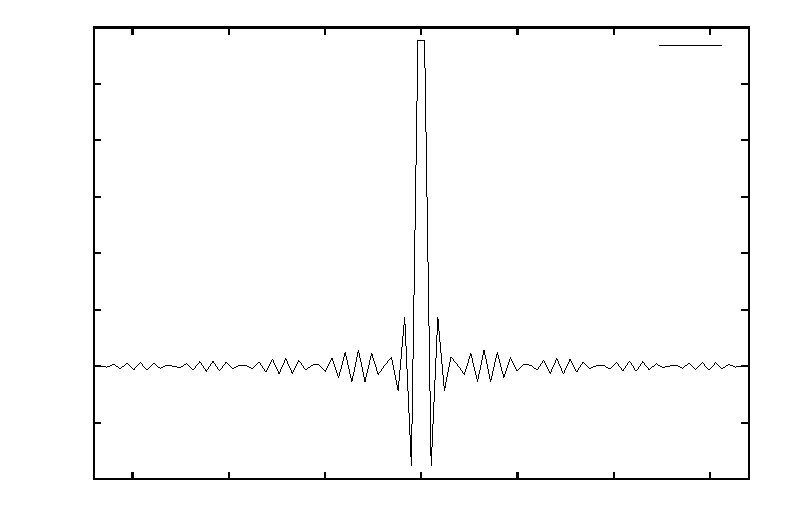
\includegraphics{function_large}}%
    \gplfronttext
  \end{picture}%
\endgroup
}
{Grafico della funzione (\ref{eq:FunzioneGnuplot}), prodotto
da \gnuplot, nell'intervallo $\cinterval{-170}{170}$.}
{fig:FunzioneGnuplotLarga}
Sicuramente il gran numero di cuspidi confligge palesemente con il fatto ben
noto che la funzione \`e in effetti derivabile su tutta la retta reale.
Eppure ci\`o che abbiamo fatto \`e cos\`i semplice (si tratta in fondo di due
soli comandi) e naturale che non \`e ovvio, a prima vista, il punto esatto in
cui abbiamo sbagliato.

La questione ci riporta per un attimo indietro ad analizzare pi\`u in dettaglio
il comando \cchar{plot}. La domanda che ci facciamo \`e, in altre parole:
che cosa fa effettivamente \gnuplot\ quando noi impartiamo un comando
\cchar{plot}?
Beh, per dirla in breve, essenzialmente divide l'intervallo di variabilit\`a
della variabile indipendente $x$%
\footnote{
Se non dichiariamo esplicitamente questo intervallo, \gnuplot\ lo sceglie da
solo, preliminarmente.
}
in un certo numero di intervalli, calcola il valore della funzione in
corrispondenza degli estremi di questi intervalli (in termini tecnici si dice
che \emph{campiona} la funzione) e quindi unisce con delle spezzate
i valori calcolati. Questo ci suggerisce che l'aspetto del grafico in figura
\ref{fig:FunzioneGnuplotLarga} possa essere in effetti dovuto ad un semplice
problema di visualizzazione, connesso con il fatto che abbiamo campionato la
funzione in modo troppo grossolano.

Leggendo la documentazione impariamo che, di \emph{default}, il numero di
di punti in cui una funzione \`e campionata per il grafico \`e
esattamente $100$. Questo numero pu\`o, come ogni altra cosa, essere
modificata dall'utente; maggiore \`e il numero di punti richiesti, pi\`u lungo
il tempo necessario per la visualizzazione, come \`e logico aspettarsi.
Ad ogni modo il comando specifico per questa operazione \`e
\cchar{set samples}, che accetta come argomento il numero di campionamenti.
Possiamo allora provare:
\begin{verbatim}
gnuplot> set samples 10000
gnuplot> set xrange [-170:170]
gnuplot> plot sin(x)/x
\end{verbatim}
ed il risultato, finalmente ragionevole, \`e mostrato in figura
\ref{fig:FunzioneGnuplotSamples}.
\panelfig
{% GNUPLOT: LaTeX picture with Postscript
\begingroup
\footnotesize
  \makeatletter
  \providecommand\color[2][]{%
    \GenericError{(gnuplot) \space\space\space\@spaces}{%
      Package color not loaded in conjunction with
      terminal option `colourtext'%
    }{See the gnuplot documentation for explanation.%
    }{Either use 'blacktext' in gnuplot or load the package
      color.sty in LaTeX.}%
    \renewcommand\color[2][]{}%
  }%
  \providecommand\includegraphics[2][]{%
    \GenericError{(gnuplot) \space\space\space\@spaces}{%
      Package graphicx or graphics not loaded%
    }{See the gnuplot documentation for explanation.%
    }{The gnuplot epslatex terminal needs graphicx.sty or graphics.sty.}%
    \renewcommand\includegraphics[2][]{}%
  }%
  \providecommand\rotatebox[2]{#2}%
  \@ifundefined{ifGPcolor}{%
    \newif\ifGPcolor
    \GPcolorfalse
  }{}%
  \@ifundefined{ifGPblacktext}{%
    \newif\ifGPblacktext
    \GPblacktexttrue
  }{}%
  % define a \g@addto@macro without @ in the name:
  \let\gplgaddtomacro\g@addto@macro
  % define empty templates for all commands taking text:
  \gdef\gplbacktext{}%
  \gdef\gplfronttext{}%
  \makeatother
  \ifGPblacktext
    % no textcolor at all
    \def\colorrgb#1{}%
    \def\colorgray#1{}%
  \else
    % gray or color?
    \ifGPcolor
      \def\colorrgb#1{\color[rgb]{#1}}%
      \def\colorgray#1{\color[gray]{#1}}%
      \expandafter\def\csname LTw\endcsname{\color{white}}%
      \expandafter\def\csname LTb\endcsname{\color{black}}%
      \expandafter\def\csname LTa\endcsname{\color{black}}%
      \expandafter\def\csname LT0\endcsname{\color[rgb]{1,0,0}}%
      \expandafter\def\csname LT1\endcsname{\color[rgb]{0,1,0}}%
      \expandafter\def\csname LT2\endcsname{\color[rgb]{0,0,1}}%
      \expandafter\def\csname LT3\endcsname{\color[rgb]{1,0,1}}%
      \expandafter\def\csname LT4\endcsname{\color[rgb]{0,1,1}}%
      \expandafter\def\csname LT5\endcsname{\color[rgb]{1,1,0}}%
      \expandafter\def\csname LT6\endcsname{\color[rgb]{0,0,0}}%
      \expandafter\def\csname LT7\endcsname{\color[rgb]{1,0.3,0}}%
      \expandafter\def\csname LT8\endcsname{\color[rgb]{0.5,0.5,0.5}}%
    \else
      % gray
      \def\colorrgb#1{\color{black}}%
      \def\colorgray#1{\color[gray]{#1}}%
      \expandafter\def\csname LTw\endcsname{\color{white}}%
      \expandafter\def\csname LTb\endcsname{\color{black}}%
      \expandafter\def\csname LTa\endcsname{\color{black}}%
      \expandafter\def\csname LT0\endcsname{\color{black}}%
      \expandafter\def\csname LT1\endcsname{\color{black}}%
      \expandafter\def\csname LT2\endcsname{\color{black}}%
      \expandafter\def\csname LT3\endcsname{\color{black}}%
      \expandafter\def\csname LT4\endcsname{\color{black}}%
      \expandafter\def\csname LT5\endcsname{\color{black}}%
      \expandafter\def\csname LT6\endcsname{\color{black}}%
      \expandafter\def\csname LT7\endcsname{\color{black}}%
      \expandafter\def\csname LT8\endcsname{\color{black}}%
    \fi
  \fi
  \setlength{\unitlength}{0.0500bp}%
  \begin{picture}(7560.00,5040.00)%
    \gplgaddtomacro\gplbacktext{%
      \csname LTb\endcsname%
      \put(770,440){\makebox(0,0)[r]{\strut{}-0.4}}%
      \put(770,1059){\makebox(0,0)[r]{\strut{}-0.2}}%
      \put(770,1679){\makebox(0,0)[r]{\strut{} 0}}%
      \put(770,2298){\makebox(0,0)[r]{\strut{} 0.2}}%
      \put(770,2918){\makebox(0,0)[r]{\strut{} 0.4}}%
      \put(770,3537){\makebox(0,0)[r]{\strut{} 0.6}}%
      \put(770,4157){\makebox(0,0)[r]{\strut{} 0.8}}%
      \put(770,4776){\makebox(0,0)[r]{\strut{} 1}}%
      \put(1272,220){\makebox(0,0){\strut{}-150}}%
      \put(2196,220){\makebox(0,0){\strut{}-100}}%
      \put(3120,220){\makebox(0,0){\strut{}-50}}%
      \put(4044,220){\makebox(0,0){\strut{} 0}}%
      \put(4968,220){\makebox(0,0){\strut{} 50}}%
      \put(5892,220){\makebox(0,0){\strut{} 100}}%
      \put(6816,220){\makebox(0,0){\strut{} 150}}%
    }%
    \gplgaddtomacro\gplfronttext{%
      \csname LTb\endcsname%
      \put(6199,4603){\makebox(0,0)[r]{\strut{}sin(x)/x}}%
    }%
    \gplbacktext
    \put(0,0){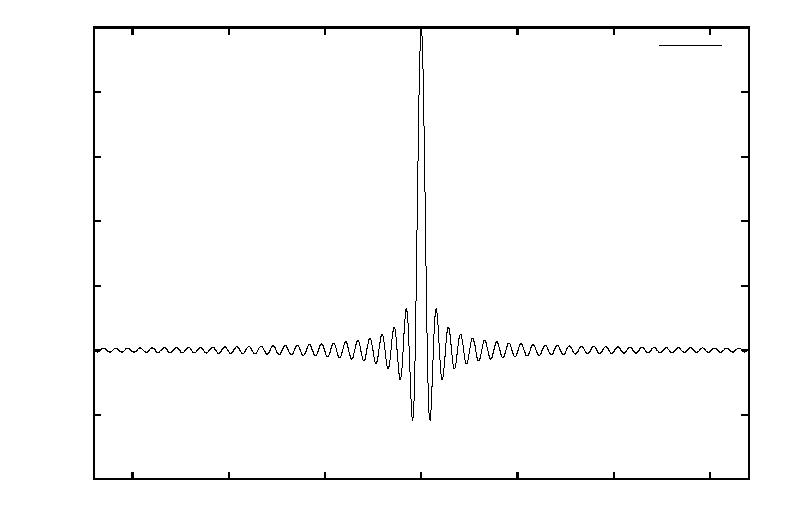
\includegraphics{function_sampled}}%
    \gplfronttext
  \end{picture}%
\endgroup
}
{Grafico della funzione (\ref{eq:FunzioneGnuplot}), prodotto
da \gnuplot, nell'intervallo $\cinterval{-170}{170}$, con un numero
di punti di campionamento pari a $10000$.}
{fig:FunzioneGnuplotSamples}

Torniamo allora per un istante a quanto detto all'inizio del paragrafo e
cerchiamo di interpretare i due ultimi grafici nel nostro nuovo schema
concettuale. In buona fede eravamo convinti di chiedere al computer di
disegnare il grafico di una funzione; in realt\`a: nel primo caso gli abbiamo
chiesto  di campionare la funzione in $100$ punti e di unire i valori ottenuti
con linee rette, mentre nel secondo gli abbiamo chiesto di fare lo stesso
campionando in $10000$ punti.
In entrambi i casi il calcolatore ha eseguito gli ordini alla lettera; il fatto
che il primo grafico non ci piaccia, mentre il secondo sia esteticamente
appagante dipende solo da noi.

Avevamo promesso esattamente \emph{due} cose meno ovvie nel titolo del
paragrafo ed ecco qui la seconda. Proviamo a digitare nella \emph{shell}
di \gnuplot\ il comando \cchar{print 1/2}.
Riuscite ad immaginare che cosa succeder\`a? Ebbene, il risultato \`e,
ancora una volta, sorprendente:
\begin{verbatim}
gnuplot> print 1/2
0
\end{verbatim}
Senza perdere troppo tempo, il punto fondamentale \`e che \gnuplot\ interpreta
numeratore e denominatore come numeri interi e restituisce pure il risultato
della divisione come intero (in effetti $0$ \`e la parte intera di
$\frac{1}{2}$).
Si tratta di una \emph{trappola} tipica in cui tutti sono caduti almeno una
volta nella vita ed \`e questo il motivo per cui l'abbiamo mostrata qui.
Se adesso rendiamo manifestamente reali il numeratore ed il denominatore,
tutto torna come ci aspettiamo:
\begin{verbatim}
gnuplot> print 1.0/2.0
0.5
\end{verbatim} 


\section{Visualizzare una serie di dati}

\gnuplot\ \`e capace di visualizzare in modo molto semplice i dati contenuti
in un \emph{file}, purch\'e organizzati per colonne e separati con spazi o
\ckey{TAB}.
Tutte le linee che cominciano con un cancelletto (\cchar{\#}) sono
automaticamente ignorate da \gnuplot\ (e tecnicamente prendono il nome di
\emph{commenti}). Questo permette, tra le altre cose, di inserire in un
generico \emph{file} di dati una breve descrizione del contenuto delle
colonne, di modo che esso sia pi\`u facilmente comprensibile. 

Supponiamo ad esempio di avere un \emph{file} di testo (denominato
\cchar{LeggeOraria.txt}) del tipo:
\begin{verbatim}
# Tempo (sec)   Posizione (cm)   Errore (cm)
5               10.1             2.0
10              17.8             1.5
15              26.6             1.5
20              32.8             2.0
25              40.2             2.5
30              47.4             2.0
\end{verbatim}
Il comando:
\begin{verbatim}
gnuplot> plot 'LeggeOraria.txt' using 1:2
\end{verbatim}
dovrebbe generare qualcosa di non troppo diverso dalla figura
\ref{fig:LeggeOraria}.
\panelfig
{\includegraphics[height=\figwidth, angle=270]%
{./ps_gnuplot/figure/LeggeOraria}}
{Visualizzazione, mediante \gnuplot, dei dati contenuti nel \emph{file}
\cchar{LeggeOraria.txt} (riportato poche righe sopra).}
{fig:LeggeOraria}
In questo contesto il comando \cchar{plot} accetta come argomento il
nome del \emph{file} di testo contenente i dati (racchiuso tra virgolette o
apici) e l'opzione \cchar{using} specifica le colonne che saranno
graficate sull'asse delle $x$ e su quello delle $y$, rispettivamente.
Si tratta di una sintassi tipica che useremo spesso; sottolineiamo anche
esplicitamente il fatto che il comando \cchar{plot} supporta una notevole
quantit\`a di opzioni, come si pu\`o facilmente verificare digitando
\cchar{help plot}.

\caution{\`E molto frequente, specialmente all'inizio, far confusione tra
percorsi relativi ed assoluti ai \emph{file}. Quando scriviamo
\cchar{plot 'LeggeOraria.txt'} assumiamo implicitamente che un \emph{file}
denominato \cchar{LeggeOraria.txt} sia presente nella \emph{directory}
corrente.}

\caution{Se non abbiamo mai usato il comando \cchar{cd} all'interno della
\emph{shell} di \gnuplot, la \emph{directory} corrente sar\`a la
\emph{directory} da cui abbiamo lanciato il programma.
In ogni caso essa pu\`o essere visualizzata tramite il comando \cchar{pwd},
anche questo da digitare nella \emph{shell} di \gnuplot.}

Quando cerchiamo di accedere ad un file che fisicamente non esiste
(o che non si trova nella posizione esatta cui stiamo puntando
all'interno del \emph{filesystem}) otteniamo in generale un messaggio d'errore.
Tanto per fissare le idee, supponiamo di aver lanciato \gnuplot\ da una certa
\emph{directory} e di avere il \emph{file} di dati \cchar{LeggeOraria.txt}
all'interno di una \emph{directory} denominata \cchar{dati} e situata a sua
volta all'interno della \emph{directory} di partenza.
Digitando il comando precedente provocheremo ovviamente un errore:
\begin{verbatim}
gnuplot> plot 'LeggeOraria.txt' using 1:2
              ^
         can't read data file "LeggeOraria.txt"
           
\end{verbatim}
perch\'e \gnuplot\ non trover\`a fisicamente il \emph{file}. Abbiamo allora
due possibilit\`a distinte: scrivere il percorso completo al \emph{file}:
\begin{verbatim}
gnuplot> plot './data/LeggeOraria.txt' using 1:2
\end{verbatim}
oppure cambiare \emph{directory} e successivamente impartire il comando
\cchar{plot}:
\begin{verbatim}
gnuplot> cd './data'
gnuplot> plot 'LeggeOraria.txt' using 1:2
\end{verbatim}

\caution{Il lettore non deve far confusione tra il comando \cchar{cd} di
\gnuplot\ ed il comando standard \ccmd{cd} di \linux. In particolare il primo
richiede che il nome della \emph{directory} di destinazione sia racchiuso
tra virgolette o apici.}

Ogni volta che si ha un messaggio di errore del tipo
\cchar{can't read data file \ldots} significa che, in un modo o nell'altro,
stiamo puntando ad un \emph{file} che fisicamente non si trova dove noi
pensiamo (o che magari non ci siamo nemmeno posti il problema).
In tal caso le cose da fare sono due: capire dove siamo
con il comando \cchar{pwd} (da digitare nella \emph{shell} di \gnuplot) e
quindi indirizzare il \emph{file} correttamente in uno dei due modi appena
mostrati.

Torniamo adesso alla nostra serie di dati e vediamo brevemente alcuni comandi
specifici di formattazione dei grafici. Supponiamo di digitare, nella
\emph{shell} di \gnuplot:
\begin{verbatim}
gnuplot> set title 'Legge oraria per una particella libera'
gnuplot> set xlabel 'Tempo (sec)'
gnuplot> set ylabel 'Posizione (cm)'
gnuplot> set xrange [0: 40]
gnuplot> set yrange [0: 50]
gnuplot> unset key
gnuplot> plot 'LeggeOraria.txt' using 1:2:3 with yerrorbars
\end{verbatim}
Il risultato \`e mostrato in figura \ref{fig:LeggeOrariaEdit}.
\panelfig
{\includegraphics[height=\figwidth, angle=270]%
{./ps_gnuplot/figure/LeggeOrariaEdit}}
{Visualizzazione, mediante \gnuplot, dei dati contenuti nel \emph{file}
\cchar{LeggeOraria.txt}, dopo alcuni semplici comandi di formattazione.}
{fig:LeggeOrariaEdit}
La maggior parte dei nuovi comandi introdotti dovrebbe essere auto-esplicativa.
In particolare dovrebbe essere chiaro come inserire il titolo del grafico,
impostare gli estremi dei due assi e mettere delle \emph{etichette} di testo
(in inglese si chiamano \emph{label}) sugli assi stessi.
Pur tuttavia commenteremo esplicitamente gli ultimi due. Il primo:
\begin{verbatim}
gnuplot> unset key
\end{verbatim}
sostanzialmente elimina la legenda, che altrimenti viene inserita nel grafico
in alto a destra (cfr. figura \ref{fig:LeggeOraria}). L'altro \`e l'usuale
comando \cchar{plot}:
\begin{verbatim}
gnuplot> plot 'LeggeOraria.txt' using 1:2:3 with yerrorbars
\end{verbatim}
che viene per\`o usato, questa volta, con l'opzione \cchar{with yerrorbars},
la quale permette di rappresentare sul grafico le barre d'errore sull'asse
delle $y$; la colonna dei valori per le barre d'errore viene passata come
terzo argomento dell'opzione \cchar{using}.
Esiste anche un'opzione \cchar{with xyerrorbars} che permette di rappresentare
le barre d'errore su entrambi gli assi; in questo caso le quattro colonne che
sono passate all'opzione \cchar{using} sono interpretate come $x$, $y$,
$\Delta x$ e $\Delta y$, rispettivamente.

\caution{Tutti i comandi di formattazione hanno effetto solamente nel momento
in cui si impartisce un nuovo comando \cchar{plot} e non prima; di converso il
loro effetto cessa solamente nel momento in cui vengono esplicitamente
sovrascritti oppure quando si esce da \gnuplot. Vale anche la pena di
menzionare il comando \cchar{replot} il quale non fa altro che ripetere
esattamente l'ultimo comando \cchar{plot}.}


\section{Realizzare un istogramma}

Diciamo subito che \gnuplot\ \emph{non} supporta la realizzazione di
istogrammi, nel senso che non ha le funzionalit\`a per creare i canali e
popolarli a partire da una serie di dati.
Pur tuttavia esiste un'opzione di \emph{visualizzazione} del comando
\cchar{plot} dedicata specificamente alla creazione istogrammi%
\footnote{
Sottolineiamo esplicitamente che si tratta solo di un opzione di
visualizzazione e che la definizione ed il popolamento dei canali debbono
essere eseguiti dall'utente.
}%
.
Senza entrare troppo nei dettagli diremo che se forniamo a \gnuplot\ un
\emph{file} di dati (supponiamo, per fissare le idee, che si chiami
\cchar{Istogramma.txt}) contenente una colonna con le coordinate
centrali dei canali ed una con il contenuto dei canali stessi, possiamo
disegnare l'istogramma corrispondente con un comando del tipo:
\begin{verbatim}
gnuplot> plot 'Istogramma.txt' using 1:2 with histeps
\end{verbatim}



\section{Salvare i grafici sotto forma di immagini}

Il lettore potr\`a chiedersi come sia stato possibile salvare i grafici
generati da \gnuplot\ in una forma che permettesse di inserirli nel paragrafo
precedente (e precisamente sotto forma di \emph{file} postscript).
Prima di mostrare esplicitamente i comandi che serviranno \`e tuttavia
necessario introdurre due concetti nuovi di fondamentale importanza:
\begin{numlist}
\item{
\cchar{output}:
\`e sostanzialmente il luogo in cui vengono mostrate (o, pi\`u precisamente
\emph{redirette}) le schermate di \gnuplot\ (in Italiano diremmo
\emph{uscita}). Nel nostro caso esso pu\`o essere, a seconda dei casi, il
monitor del calcolatore oppure un \emph{file}%
\footnote{
Vi sono in effetti alcune altre possibilit\`a un poco pi\`u esotiche che
potete trovare nella documentazione specifica.
}%
.
Vedremo tra breve come passare da una modalit\`a all'altra.
}
\item{
\cchar{terminal}:
\`e il \emph{linguaggio} con cui le schermate di \gnuplot\ vengono redirette
sull'uscita (qualunque essa sia). Nel caso l'uscita sia un \emph{file}, questo
linguaggio pu\`o essere, ad esempio postscript, gif, png, etc.
Nel caso in cui invece vogliamo, come accade tipicamente, le schermate
sul monitor, questo linguaggio sar\`a, in un qualche senso, il
linguaggio del sistema operativo; come vedremo nel seguito, il nome da usare
sar\`a \cchar{x11} sotto \linux\ e \cchar{windows} sotto \windows.
}
\end{numlist}

A questo punto non dovrebbe essere troppo difficile capire come si possa
salvare un grafico sotto forma di immagine: dovremo redirigere l'uscita su di
un \emph{file} specifico ed impostare opportunamente il terminale.
Vale a dire qualcosa del genere:
\begin{verbatim}
gnuplot> set terminal postscript
gnuplot> set output 'Immagine.eps'
gnuplot> replot
gnuplot> set output
gnuplot> set terminal x11
\end{verbatim}

\caution{I comandi \cchar{set output} e \cchar{set terminal} non sono
indipendenti l'uno dall'altro: non tutti i terminali sono appropriati per
tutti i tipi di \emph{output} e viceversa.
Il lettore potr\`a divertirsi, per curiosit\`a, a provare alcune delle
combinazioni \emph{proibite} (come terminale postscript su \emph{output}
standard oppure terminale \cchar{x11} su di un \emph{file}).
Gli effetti saranno interessanti.}

Analizziamo i comandi appena scritti uno per uno, alla luce di quanto detto
sino ad ora. I primi due
\begin{verbatim}
gnuplot> set terminal postscript
gnuplot> set output 'Immagine.eps'
\end{verbatim}
redirigono l'uscita su di una \emph{file} che si chiamer\`a
\cchar{Immagine.eps}%
\footnote{
Se non specifichiamo il percorso completo il \emph{file} verr\`a creato nella
\emph{directory} corrente. \`E importante anche notare che, nel caso esista
gi\`a un \emph{file} con lo stesso nome, esso verr\`a sovrascritto senza che ne
venga richiesta conferma.
}
e che verr\`a scritto in linguaggio postscript, come specificato nella
impostazione del terminale.
Il comando successivo:
\begin{verbatim}
gnuplot> replot
\end{verbatim}
esegue di nuovo l'ultimo comando plot che \`e stato digitato. In questo caso,
essendo l'\emph{output} rediretto su \emph{file}, il grafico non apparir\`a
sullo schermo; al contrario verr\`a fisicamente \emph{scritto} sul \emph{file}
stesso. Quando torniamo sull'\emph{output} standard, vale a dire sullo schermo
del calcolatore:
\begin{verbatim}
gnuplot> set output
\end{verbatim}
il \emph{file} di uscita viene \emph{chiuso}. L'ultimo comando permette di
impostare di nuovo il terminale nella modalit\`a di default:
\begin{verbatim}
gnuplot> set terminal x11
\end{verbatim}
e siamo di nuovo al punto di partenza, in cui i comandi \cchar{plot} producono
bellissimi grafici sullo schermo. Vale la pena notare che, se lavorassimo sotto
\windows, quest'ultimo comando (e solo questo) sarebbe diverso:
\begin{verbatim}
gnuplot> set terminal windows
\end{verbatim}


\section{Il concetto di macro}

Adesso che il nostro vocabolario, in termini di comandi di \gnuplot, si \`e
fatto abbastanza ampio da consentirci di produrre una certa quantit\`a di cose
interessanti, diventa davvero indispensabile introdurre il concetto di
\emph{macro}. In termini semplici una macro \`e una sequenza di comandi
(validi) inseriti, uno dopo l'altro, in un \emph{file} di testo.
Il vantaggio fondamentale del lavorare con le macro \`e che, mentre tutti i
comandi che digitiamo nel prompt vanno perduti non appena usciamo dal
programma, una macro, una volta salvata, pu\`o essere riutilizzata
(eventualmente dopo modifiche) a distanza di tempo. Come vedremo, \`e
sufficiente un solo comando per eseguirla.

Una tipica macro che utilizzi i comandi imparati sino ad ora potrebbe apparire
come segue:
\begin{verbatim}
# Inizializzazione.
set output
set terminal x11

# Definizione e formattazione del grafico.
set title 'Legge oraria per una particella libera'
set xlabel 'Tempo (sec)'
set ylabel 'Posizione (cm)'
set xrange [0: 40]
set yrange [0: 50]
unset key
plot 'LeggeOraria.txt' using 1:2:3 with yerrorbars

# Creazione del file di uscita.
set terminal postscript
set output 'Immagine.eps'
replot

# Ritorno allo schermo.
set output
set terminal x11
\end{verbatim}

Dato che, come gi\`a sappiamo, le linee che cominciano con un cancelletto
vengono ignorate da \gnuplot, nella macro qui sopra ne abbiamo usate alcune per
commentare la macro stessa. Si tratta di una buona abitudine che, unita all'uso
di linee vuote per separare blocchi logici distinti, aumenta la
leggibilit\`a.
Notiamo esplicitamente come i primi due comandi:
\begin{verbatim}
gnuplot> set output
gnuplot> set terminal x11
\end{verbatim}
pur se non formalmente necessari, costituiscano pure una buona abitudine,
che pu\`o salvare da apparenti inconsistenze nel caso in cui le impostazioni
di partenza non siano, per qualche ragione, quelle che ci aspettiamo. 

Supponendo dunque che il \emph{file} di testo in cui abbiamo salvato la macro
si chiami \cchar{macro.txt}, essa si esegue digitando nella \emph{shell} di
\gnuplot:
\begin{verbatim}
gnuplot> load 'macro.txt'
\end{verbatim}
Questo dovrebbe produrre sostanzialmente la figura \ref{fig:LeggeOrariaEdit}.


\section{Eseguire un fit ad una serie di dati}

\gnuplot\ permette di eseguire un fit del minimo $\chi^2$ ad una serie di dati%
\footnote{
Per essere precisi, \gnuplot\ utilizza una propria implementazione
dell'algoritmo di Marquardt-Levenberg per il fit non lineare dei minimi
quadrati (NLLS). I punti sono pesati con l'inverso del loro errore, per cui
questo metodo \`e in effetti concettualmente affine a quello che noi
conosciamo come metodo del minimo $\chi^2$.
}
con una generica funzione definita dall'utente. I comandi coinvolti in questa
operazione sono, pi\`u o meno, i seguenti:
\begin{verbatim}
gnuplot> f(x) = a + b*x
gnuplot> a = 1
gnuplot> b = 1
gnuplot> fit f(x) 'LeggeOraria.txt' using 1:2:3 via a, b 
\end{verbatim}
Al solito li analizzeremo brevemente uno ad uno. Il primo:
\begin{verbatim}
gnuplot> f(x) = a + b*x
\end{verbatim}
definisce la funzione con cui vogliamo eseguire il fit. In questo caso \`e
semplicemente una retta, ma si possono utilizzare tutte le funzioni predefinite
in \gnuplot, eventualmente combinate attraverso gli operatori in tabella
\ref{tab:OperatoriGnuplot}. Il che \`e sufficiente per la stragrande
maggioranza delle applicazioni.
I due comandi successivi:
\begin{verbatim}
gnuplot> a = 1
gnuplot> b = 1
\end{verbatim}
inizializzano i parametri della funzione con cui si fa il fit.

\caution{Il modo in cui il calcolatore esegue un fit \`e, per molti aspetti,
\emph{diverso} da come faremmo noi, seguendo i metodi descritti nel capitolo
\ref{chap:fit}. In particolare, anche nei casi in cui le equazioni a cui porta
il metodo del minimo $\chi^2$ si possono risolvere analiticamente, il
calcolatore utilizza dei metodi numerici per cui i valori iniziali dei
parametri sono essenziali. Vi sono casi, nemmeno troppi complicati, in cui il
fit pu\`o convergere o non convergere, a seconda di come inizializziamo i
parametri. Vi sono anche casi, per certi versi ancor pi\`u pericolosi, in cui
valori iniziali diversi fanno convergere il fit a valori finali diversi.
In ogni caso, \`e una buona abitudine fornire una stima sensata dei parametri
(magari solo guardando il grafico) prima di cominciare il fit.}

\noindent L'ultimo comando:
\begin{verbatim}
gnuplot> fit f(x) 'LeggeOraria.txt' using 1:2:3 via a, b
\end{verbatim}
\`e quello che esegue il fit propriamente detto. Esso accetta come parametro la
funzione con cui fittare i dati ed il nome del \emph{file} in cui i dati
stessi sono contenuti.
Le tre colonne che vengono passate all'opzione \cchar{using} sono interpretate
come valori della $x$, della $y$ e degli errori sulla $y$, rispettivamente
La terza colonna (quella degli errori sulla $y$) non \`e strettamente
richiesta.

\caution{Se gli errori sulla $y$ non vengono forniti, \gnuplot\ assume
che essi siano tutti pari ad $1$; questo \`e rilevante (\`e importante
ricordarlo) per il valore del $\chi^2$ che, come vedremo, il fit fornisce
come sottoprodotto); \gnuplot\ \emph{non} supporta fit di tipo generale
(vale a dire con errori su entrambe le variabili).}

\noindent L'opzione \cchar{via} definisce quali tra i parametri della funzione
siano liberi di variare durante il fit (quelli che eventualmente non sono
menzionati sono considerati fissi al loro valore iniziale).

Se le cose non fossero ancora perfettamente chiare, la macro seguente:
\begin{verbatim}
# Inizializzazione.
set output
set terminal x11

# Definizione e formattazione del grafico.
set title 'Legge oraria per una particella libera'
set xlabel 'Tempo (sec)'
set ylabel 'Posizione (cm)'
set xrange [0: 40]
set yrange [0: 50]
unset key

# Esecuzione del fit
f(x) = a + b*x
a = 1
b = 1
fit f(x) 'LeggeOraria.txt' using 1:2:3 via a, b

# Creazione del grafico.
plot 'LeggeOraria.txt' using 1:2:3 with yerrorbars, f(x)

# Creazione del file di uscita.
set terminal postscript
set output 'Immagine.eps'
replot

# Ritorno allo schermo.
set output
set terminal x11
\end{verbatim}
dovrebbe produrre, ammesso che tutto funzioni correttamente, il grafico in
figura
\ref{fig:LeggeOrariaFit}.
\panelfig
{\includegraphics[height=\figwidth, angle=270]%
{./ps_gnuplot/figure/LeggeOrariaFit}}
{Grafico prodotto dalla macro riportata in questa sezione.}
{fig:LeggeOrariaFit}
Notiamo come il comando \cchar{plot} permetta di graficare pi\`u oggetti (in
questo caso una serie di dati ed una funzione), a patto che essi siano separati
da una virgola.

Contestualmente al grafico (mostrato sullo schermo e salvato su di un
\emph{file}) il comando \cchar{fit} produrr\`a una serie di linee sul
terminale di \gnuplot, contenenti informazioni sull'esito del fit stesso%
\footnote{
Queste informazioni sono anche salvate, per futura referenza, su un
\emph{file} di testo chiamato \cchar{fit.log} e salvato nella \emph{directory}
corrente.
}%
:
\begin{verbatim}
***********************************************************
Wed Feb 12 09:45:22 2003


FIT:    data read from 'LeggeOraria.txt' using 1:2:3
        #datapoints = 6
function used for fitting: f(x)
fitted parameters initialized with current variable values



Iteration 0
WSSR        : 209.004           delta(WSSR)/WSSR   : 0
delta(WSSR) : 0                 limit for stopping : 1e-05
lambda    : 6.93718

initial set of free parameter values

a               = 1
b               = 1

After 5 iterations the fit converged.
final sum of squares of residuals : 0.686015
rel. change during last iteration : -2.87956e-12

degrees of freedom (ndf) : 4
rms of residuals      (stdfit) = sqrt(WSSR/ndf)      : 0.41413
variance of residuals (reduced chisquare) = WSSR/ndf : 0.171504

Final set of parameters            Asymptotic Standard Error
=======================            ==========================

a               = 3.25533          +/- 0.698        (21.44%)
b               = 1.48589          +/- 0.03902      (2.626%)


correlation matrix of the fit parameters:

               a      b
a               1.000
b              -0.897  1.000
\end{verbatim}
Le informazioni pi\`u importanti sono i valori finali dei parametri che
si trovano dopo la riga:
\begin{verbatim}
Final set of parameters            Asymptotic Standard Error
=======================            ==========================

a               = 3.25533          +/- 0.698        (21.44%)
b               = 1.48589          +/- 0.03902      (2.626%)
\end{verbatim}
la matrice di correlazione dei parametri, che abbiamo definito nel
paragrafo \ref{sec:Correlazione} e che leggiamo sotto la riga:
\begin{verbatim}
correlation matrix of the fit parameters:

               a      b
a               1.000
b              -0.897  1.000
\end{verbatim}
ed il valore del $\chi^2$ diviso il numero di gradi di libert\`a:
\begin{verbatim}
variance of residuals (reduced chisquare) = WSSR/ndf : 0.171504
\end{verbatim}
Vale la pena di ricordare che, nel caso in cui non si specifichi esplicitamente
una colonna di dati contenente gli errori sulle $y$, il valore del $\chi^2$(che
\gnuplot\ fornisce comunque) perde completamente di significato (in tal caso,
come abbiamo gi\`a detto, il programma assume semplicemente che tutti gli
errori siano pari all'unit\`a).

Come commento finale vorremmo sottolineare che il fatto che il calcolatore
scriva esplicitamente:
\begin{verbatim}
a               = 3.25533          +/- 0.698        (21.44%)
\end{verbatim}
non ci autorizza a dimenticare le regole consuete sulle cifre significative.
Noi scriveremo sempre:
$$
a = 3.25 \pm 0.70
$$


\section{Operazioni con le colonne}

Vi \`e un'ultima cosa che, essendo utile in molte situazioni, vale la pena
di discutere brevemente e si tratta delle operazioni che \gnuplot\ consente
di eseguire con le colonne di un generico \emph{file} di dati.

Supponiamo, per fissare le idee, di avere un \emph{file} di dati (come al
solito organizzato per colonne) e di voler fare un grafico con la colonna
numero $1$ sull'asse delle $x$ ed il \emph{quadrato} della colonna numero $2$
su quello delle $y$. Ebbene, in questo caso scriveremmo:
\begin{verbatim}
gnuplot> plot 'LeggeOraria.txt' using 1:(($2)**2)
\end{verbatim}
Non \`e il caso, di nuovo, di dilungarsi in spiegazioni. Essenzialmente
la scrittura \cchar{(\$2)} identifica la seconda colonna come oggetto nel suo
insieme; dopo di che si pu\`o utilizzare la consueta sintassi (cio\`e le
funzioni e gli operatori che gi\`a conosciamo) per fare operazioni sulle
colonne stesse, elemento per elemento.
A volte, specialmente se le operazioni da fare sulle colonne sono complesse,
se   si vuole vedere il risultato di tali operazioni (quanto meno come
controllo che tutto proceda correttamente) conviene generare un \emph{file} di
dati trasformati (utilizzando un programma che lo consenta, come \scilab) e
quindi lavorare su di essi.


\appendix

% Appendici.
\chapter{Tavole numeriche}
\label{chap:TavoleNumeriche}

\section{Definizione della funzione \texorpdfstring{$\erf(x)$}{erf}}
\label{app:Erf}

La funzione $\erf$ (nota anche come {\itshape error function}) \`e
solitamente definita%
\footnote
{
Purtroppo alcuni autori preferiscono definire la funzione erf come:
\begin{equation}\label{eq:Erf}
\Erf(x) = \frac{2}{\sqrt{\pi}} \dintegral{e^{-\xi^2}}{\xi}{0}{x}
\end{equation}
che \`e legata alla \ref{eq:erf} da un semplice cambio di variabile:
\begin{equation}
\erf(x) = \frac{1}{2} \Erf \left( \frac{x}{\sqrt{2}} \right)
\end{equation}
Prima di utilizzare delle tavole numeriche \`e dunque essenziale
verificarne il significato esatto.
}
come:
\begin{equation}\label{eq:erf}
\erf(x) = \frac{1}{\sqrt{2\pi}} \dintegral{e^{-\xi^2/2}}{\xi}{0}{x}
\end{equation}
ed \`e essenzialmente l'integrale, eseguito tra 0 ed un estremo
variabile $x$, di una distribuzione Gaussiana di media 0 e deviazione
standard 1:
\begin{equation}
\erf(x) = \dintegral{G(z)}{z}{0}{x}
\end{equation}
\panelfig
{\onebyonetexfig{./aa_tabelle/figure/erf.tex}}
{Grafico della funzione $\erf(x)$ definita dall'equazione \ref{eq:erf}.}
{fig:Erf}

\begin{exemplify}

\example{$\erf(1) = 0.3413$. Questo significa che la probabilit\`a che il
valore di una variabile Gaussiana standard sia compreso tra $0$ ed $1$ vale
$0.3413$.\\
Il risultato pu\`o essere facilmente generalizzato ad una qualsiasi
distribuzione Gaussiana: la probabilit\`a che la variabile sia compresa tra
$\mu$ ($0$ per la variabile standard) e $\mu + \sigma$ ($0 + 1 = 1$ per la
variabile standard) vale $0.3413$.}

\example{Se moltiplichiamo per due il valore appena trovato
($0.3413 \cdot 2 = 0.6826$) riotteniamo il ben noto risultato che la
probabilit\`a che una variabile gaussiana disti meno di una deviazione
standard dal suo valor medio \`e circa il 68\%.}

\end{exemplify}

Nel capitolo \ref{chap:Distribuzioni} abbiamo gi\`a anticipato che questo
integrale (che rappresenta la probabilit\`a di trovare una variabile normale
in forma standard entro l'intervallo $\cinterval{0}{x}$) non ha espressione
analitica e deve essere valutato numericamente.
La funzione $\erf$ si trova tabulata qui di seguito per un insieme
significativo di valori di $x$.
Il procedimento base per estrarre dalle tavole i valori di probabilit\`a
\`e stato gi\`a descritto nel capitolo \ref{chap:Distribuzioni} e \`e
sostanzialmente fondato sulla relazione, valida per una variabile Gaussiana
standard%
\footnote{
Alcuni dei programmi di analisi dati comunemente usati (ad esempio scilab e
\gnuplot) utilizzano la definizione (\ref{eq:Erf}).
In questo caso si ha, ovviamente:
$$
\prob{a \leq x \leq b} =
\frac{1}{2} \left[ \Erf\left(\frac{b}{\sqrt{2}}\right) -
\Erf\left(\frac{a}{\sqrt{2}}\right) \right]
$$
}%
:
\begin{equation}\label{eq:ProbErf}
\prob{a \leq x \leq b} = \erf(b) - \erf(a)
\end{equation}
Per una distribuzione Gaussiana con media e deviazione standard arbitrarie
la (\ref{eq:ProbErf}) pu\`o ancora essere utilizzata passando alla variabile
in forma standard (cfr. capitolo \ref{chap:Distribuzioni}).

\section{Integrale normale degli errori - I}
\label{app:Erf1}

\tabhdr
{./aa_tabelle/figure/gauss_integral.tex}
{Tavole della funzione $f(x) = \erf(x)$.
\vskip\baselineskip
{\footnotesize Nota: le righe identificano le prime due cifre della $x$, mentre
le colonne identificano la seconda cifra decimale della $x$ stessa.}}
{la probabilit\`a che una variabile gaussiana standard sia compresa
tra $0.0$ e $1.52$ \`e $0.43574$ (cfr.~sedicesima riga, terza colonna).}

% Generated by Table.py on Mon Aug 25 16:05:42 2008.

\begin{table}[htb!]
\begin{center}
{\scriptsize
\renewcommand\arraystretch{1.250000}
\begin{tabular}{p{22 pt}cccccccccc}
\hline

\rule[-2pt]{0pt}{14pt}$x$ & $0$ & $1$ & $2$ & $3$ & $4$ & $5$ & $6$ & $7$ & $8$ & $9$\\
\hline
\hline
\rule[0pt]{0pt}{15pt}$0.0$ & $0.00000$ & $0.00399$ & $0.00798$ & $0.01197$ & $0.01595$ & $0.01994$ & $0.02392$ & $0.02790$ & $0.03188$ & $0.03586$\\
$0.1$ & $0.03983$ & $0.04380$ & $0.04776$ & $0.05172$ & $0.05567$ & $0.05962$ & $0.06356$ & $0.06749$ & $0.07142$ & $0.07535$\\
$0.2$ & $0.07926$ & $0.08317$ & $0.08706$ & $0.09095$ & $0.09483$ & $0.09871$ & $0.10257$ & $0.10642$ & $0.11026$ & $0.11409$\\
$0.3$ & $0.11791$ & $0.12172$ & $0.12552$ & $0.12930$ & $0.13307$ & $0.13683$ & $0.14058$ & $0.14431$ & $0.14803$ & $0.15173$\\
$0.4$ & $0.15542$ & $0.15910$ & $0.16276$ & $0.16640$ & $0.17003$ & $0.17364$ & $0.17724$ & $0.18082$ & $0.18439$ & $0.18793$\\
$0.5$ & $0.19146$ & $0.19497$ & $0.19847$ & $0.20194$ & $0.20540$ & $0.20884$ & $0.21226$ & $0.21566$ & $0.21904$ & $0.22240$\\
$0.6$ & $0.22575$ & $0.22907$ & $0.23237$ & $0.23565$ & $0.23891$ & $0.24215$ & $0.24537$ & $0.24857$ & $0.25175$ & $0.25490$\\
$0.7$ & $0.25804$ & $0.26115$ & $0.26424$ & $0.26730$ & $0.27035$ & $0.27337$ & $0.27637$ & $0.27935$ & $0.28230$ & $0.28524$\\
$0.8$ & $0.28814$ & $0.29103$ & $0.29389$ & $0.29673$ & $0.29955$ & $0.30234$ & $0.30511$ & $0.30785$ & $0.31057$ & $0.31327$\\
$0.9$ & $0.31594$ & $0.31859$ & $0.32121$ & $0.32381$ & $0.32639$ & $0.32894$ & $0.33147$ & $0.33398$ & $0.33646$ & $0.33891$\\
$1.0$ & $0.34134$ & $0.34375$ & $0.34614$ & $0.34849$ & $0.35083$ & $0.35314$ & $0.35543$ & $0.35769$ & $0.35993$ & $0.36214$\\
$1.1$ & $0.36433$ & $0.36650$ & $0.36864$ & $0.37076$ & $0.37286$ & $0.37493$ & $0.37698$ & $0.37900$ & $0.38100$ & $0.38298$\\
$1.2$ & $0.38493$ & $0.38686$ & $0.38877$ & $0.39065$ & $0.39251$ & $0.39435$ & $0.39617$ & $0.39796$ & $0.39973$ & $0.40147$\\
$1.3$ & $0.40320$ & $0.40490$ & $0.40658$ & $0.40824$ & $0.40988$ & $0.41149$ & $0.41309$ & $0.41466$ & $0.41621$ & $0.41774$\\
$1.4$ & $0.41924$ & $0.42073$ & $0.42220$ & $0.42364$ & $0.42507$ & $0.42647$ & $0.42785$ & $0.42922$ & $0.43056$ & $0.43189$\\
$1.5$ & $0.43319$ & $0.43448$ & $0.43574$ & $0.43699$ & $0.43822$ & $0.43943$ & $0.44062$ & $0.44179$ & $0.44295$ & $0.44408$\\
$1.6$ & $0.44520$ & $0.44630$ & $0.44738$ & $0.44845$ & $0.44950$ & $0.45053$ & $0.45154$ & $0.45254$ & $0.45352$ & $0.45449$\\
$1.7$ & $0.45543$ & $0.45637$ & $0.45728$ & $0.45818$ & $0.45907$ & $0.45994$ & $0.46080$ & $0.46164$ & $0.46246$ & $0.46327$\\
$1.8$ & $0.46407$ & $0.46485$ & $0.46562$ & $0.46638$ & $0.46712$ & $0.46784$ & $0.46856$ & $0.46926$ & $0.46995$ & $0.47062$\\
$1.9$ & $0.47128$ & $0.47193$ & $0.47257$ & $0.47320$ & $0.47381$ & $0.47441$ & $0.47500$ & $0.47558$ & $0.47615$ & $0.47670$\\
$2.0$ & $0.47725$ & $0.47778$ & $0.47831$ & $0.47882$ & $0.47932$ & $0.47982$ & $0.48030$ & $0.48077$ & $0.48124$ & $0.48169$\\
$2.1$ & $0.48214$ & $0.48257$ & $0.48300$ & $0.48341$ & $0.48382$ & $0.48422$ & $0.48461$ & $0.48500$ & $0.48537$ & $0.48574$\\
$2.2$ & $0.48610$ & $0.48645$ & $0.48679$ & $0.48713$ & $0.48745$ & $0.48778$ & $0.48809$ & $0.48840$ & $0.48870$ & $0.48899$\\
$2.3$ & $0.48928$ & $0.48956$ & $0.48983$ & $0.49010$ & $0.49036$ & $0.49061$ & $0.49086$ & $0.49111$ & $0.49134$ & $0.49158$\\
$2.4$ & $0.49180$ & $0.49202$ & $0.49224$ & $0.49245$ & $0.49266$ & $0.49286$ & $0.49305$ & $0.49324$ & $0.49343$ & $0.49361$\\
$2.5$ & $0.49379$ & $0.49396$ & $0.49413$ & $0.49430$ & $0.49446$ & $0.49461$ & $0.49477$ & $0.49492$ & $0.49506$ & $0.49520$\\
$2.6$ & $0.49534$ & $0.49547$ & $0.49560$ & $0.49573$ & $0.49585$ & $0.49598$ & $0.49609$ & $0.49621$ & $0.49632$ & $0.49643$\\
$2.7$ & $0.49653$ & $0.49664$ & $0.49674$ & $0.49683$ & $0.49693$ & $0.49702$ & $0.49711$ & $0.49720$ & $0.49728$ & $0.49736$\\
$2.8$ & $0.49744$ & $0.49752$ & $0.49760$ & $0.49767$ & $0.49774$ & $0.49781$ & $0.49788$ & $0.49795$ & $0.49801$ & $0.49807$\\
$2.9$ & $0.49813$ & $0.49819$ & $0.49825$ & $0.49831$ & $0.49836$ & $0.49841$ & $0.49846$ & $0.49851$ & $0.49856$ & $0.49861$\\
\hline

\end{tabular}
}
\end{center}
\end{table}
\vfill
\hfill {\scriptsize Generato in 0.291 s il 25 Agosto 2008 alle ore 16:05.}


\section{Integrale normale degli errori - II}
\label{app:Erf2}

\tabhdr
{./aa_tabelle/figure/gauss_integral_inverse.tex}
{Tavole della funzione $f(x) = 0.5 - \erf(x)$.
\vskip\baselineskip
{\footnotesize Nota: le righe identificano le prime due cifre della $x$, mentre
le colonne identificano la seconda cifra decimale della $x$ stessa.}}
{la probabilit\`a che una variabile gaussiana in forma standard sia
maggiore di $3.32$ \`e $4.50 \cdot 10^{-4}$ (cfr.~quarta riga, terza colonna).}

% Generated by Table.py on Mon Aug 25 16:05:42 2008.

\begin{table}[htb!]
\begin{center}
{\scriptsize
\renewcommand\arraystretch{1.250000}
\begin{tabular}{p{22 pt}cccccccccc}
\hline

\rule[-2pt]{0pt}{14pt}$x$ & $0$ & $1$ & $2$ & $3$ & $4$ & $5$ & $6$ & $7$ & $8$ & $9$\\
\hline
\hline
\rule[0pt]{0pt}{15pt}$3.0$ & $1.35\,{\rm e}$-$3$ & $1.31\,{\rm e}$-$3$ & $1.26\,{\rm e}$-$3$ & $1.22\,{\rm e}$-$3$ & $1.18\,{\rm e}$-$3$ & $1.14\,{\rm e}$-$3$ & $1.11\,{\rm e}$-$3$ & $1.07\,{\rm e}$-$3$ & $1.04\,{\rm e}$-$3$ & $1.00\,{\rm e}$-$3$\\
$3.1$ & $9.68\,{\rm e}$-$4$ & $9.35\,{\rm e}$-$4$ & $9.04\,{\rm e}$-$4$ & $8.74\,{\rm e}$-$4$ & $8.45\,{\rm e}$-$4$ & $8.16\,{\rm e}$-$4$ & $7.89\,{\rm e}$-$4$ & $7.62\,{\rm e}$-$4$ & $7.36\,{\rm e}$-$4$ & $7.11\,{\rm e}$-$4$\\
$3.2$ & $6.87\,{\rm e}$-$4$ & $6.64\,{\rm e}$-$4$ & $6.41\,{\rm e}$-$4$ & $6.19\,{\rm e}$-$4$ & $5.98\,{\rm e}$-$4$ & $5.77\,{\rm e}$-$4$ & $5.57\,{\rm e}$-$4$ & $5.38\,{\rm e}$-$4$ & $5.19\,{\rm e}$-$4$ & $5.01\,{\rm e}$-$4$\\
$3.3$ & $4.83\,{\rm e}$-$4$ & $4.66\,{\rm e}$-$4$ & $4.50\,{\rm e}$-$4$ & $4.34\,{\rm e}$-$4$ & $4.19\,{\rm e}$-$4$ & $4.04\,{\rm e}$-$4$ & $3.90\,{\rm e}$-$4$ & $3.76\,{\rm e}$-$4$ & $3.62\,{\rm e}$-$4$ & $3.49\,{\rm e}$-$4$\\
$3.4$ & $3.37\,{\rm e}$-$4$ & $3.25\,{\rm e}$-$4$ & $3.13\,{\rm e}$-$4$ & $3.02\,{\rm e}$-$4$ & $2.91\,{\rm e}$-$4$ & $2.80\,{\rm e}$-$4$ & $2.70\,{\rm e}$-$4$ & $2.60\,{\rm e}$-$4$ & $2.51\,{\rm e}$-$4$ & $2.42\,{\rm e}$-$4$\\
$3.5$ & $2.33\,{\rm e}$-$4$ & $2.24\,{\rm e}$-$4$ & $2.16\,{\rm e}$-$4$ & $2.08\,{\rm e}$-$4$ & $2.00\,{\rm e}$-$4$ & $1.93\,{\rm e}$-$4$ & $1.85\,{\rm e}$-$4$ & $1.78\,{\rm e}$-$4$ & $1.72\,{\rm e}$-$4$ & $1.65\,{\rm e}$-$4$\\
$3.6$ & $1.59\,{\rm e}$-$4$ & $1.53\,{\rm e}$-$4$ & $1.47\,{\rm e}$-$4$ & $1.42\,{\rm e}$-$4$ & $1.36\,{\rm e}$-$4$ & $1.31\,{\rm e}$-$4$ & $1.26\,{\rm e}$-$4$ & $1.21\,{\rm e}$-$4$ & $1.17\,{\rm e}$-$4$ & $1.12\,{\rm e}$-$4$\\
$3.7$ & $1.08\,{\rm e}$-$4$ & $1.04\,{\rm e}$-$4$ & $9.96\,{\rm e}$-$5$ & $9.57\,{\rm e}$-$5$ & $9.20\,{\rm e}$-$5$ & $8.84\,{\rm e}$-$5$ & $8.50\,{\rm e}$-$5$ & $8.16\,{\rm e}$-$5$ & $7.84\,{\rm e}$-$5$ & $7.53\,{\rm e}$-$5$\\
$3.8$ & $7.23\,{\rm e}$-$5$ & $6.95\,{\rm e}$-$5$ & $6.67\,{\rm e}$-$5$ & $6.41\,{\rm e}$-$5$ & $6.15\,{\rm e}$-$5$ & $5.91\,{\rm e}$-$5$ & $5.67\,{\rm e}$-$5$ & $5.44\,{\rm e}$-$5$ & $5.22\,{\rm e}$-$5$ & $5.01\,{\rm e}$-$5$\\
$3.9$ & $4.81\,{\rm e}$-$5$ & $4.61\,{\rm e}$-$5$ & $4.43\,{\rm e}$-$5$ & $4.25\,{\rm e}$-$5$ & $4.07\,{\rm e}$-$5$ & $3.91\,{\rm e}$-$5$ & $3.75\,{\rm e}$-$5$ & $3.59\,{\rm e}$-$5$ & $3.45\,{\rm e}$-$5$ & $3.30\,{\rm e}$-$5$\\
$4.0$ & $3.17\,{\rm e}$-$5$ & $3.04\,{\rm e}$-$5$ & $2.91\,{\rm e}$-$5$ & $2.79\,{\rm e}$-$5$ & $2.67\,{\rm e}$-$5$ & $2.56\,{\rm e}$-$5$ & $2.45\,{\rm e}$-$5$ & $2.35\,{\rm e}$-$5$ & $2.25\,{\rm e}$-$5$ & $2.16\,{\rm e}$-$5$\\
$4.1$ & $2.07\,{\rm e}$-$5$ & $1.98\,{\rm e}$-$5$ & $1.89\,{\rm e}$-$5$ & $1.81\,{\rm e}$-$5$ & $1.74\,{\rm e}$-$5$ & $1.66\,{\rm e}$-$5$ & $1.59\,{\rm e}$-$5$ & $1.52\,{\rm e}$-$5$ & $1.46\,{\rm e}$-$5$ & $1.39\,{\rm e}$-$5$\\
$4.2$ & $1.33\,{\rm e}$-$5$ & $1.28\,{\rm e}$-$5$ & $1.22\,{\rm e}$-$5$ & $1.17\,{\rm e}$-$5$ & $1.12\,{\rm e}$-$5$ & $1.07\,{\rm e}$-$5$ & $1.02\,{\rm e}$-$5$ & $9.77\,{\rm e}$-$6$ & $9.34\,{\rm e}$-$6$ & $8.93\,{\rm e}$-$6$\\
$4.3$ & $8.54\,{\rm e}$-$6$ & $8.16\,{\rm e}$-$6$ & $7.80\,{\rm e}$-$6$ & $7.46\,{\rm e}$-$6$ & $7.12\,{\rm e}$-$6$ & $6.81\,{\rm e}$-$6$ & $6.50\,{\rm e}$-$6$ & $6.21\,{\rm e}$-$6$ & $5.93\,{\rm e}$-$6$ & $5.67\,{\rm e}$-$6$\\
$4.4$ & $5.41\,{\rm e}$-$6$ & $5.17\,{\rm e}$-$6$ & $4.94\,{\rm e}$-$6$ & $4.71\,{\rm e}$-$6$ & $4.50\,{\rm e}$-$6$ & $4.29\,{\rm e}$-$6$ & $4.10\,{\rm e}$-$6$ & $3.91\,{\rm e}$-$6$ & $3.73\,{\rm e}$-$6$ & $3.56\,{\rm e}$-$6$\\
$4.5$ & $3.40\,{\rm e}$-$6$ & $3.24\,{\rm e}$-$6$ & $3.09\,{\rm e}$-$6$ & $2.95\,{\rm e}$-$6$ & $2.81\,{\rm e}$-$6$ & $2.68\,{\rm e}$-$6$ & $2.56\,{\rm e}$-$6$ & $2.44\,{\rm e}$-$6$ & $2.32\,{\rm e}$-$6$ & $2.22\,{\rm e}$-$6$\\
$4.6$ & $2.11\,{\rm e}$-$6$ & $2.01\,{\rm e}$-$6$ & $1.92\,{\rm e}$-$6$ & $1.83\,{\rm e}$-$6$ & $1.74\,{\rm e}$-$6$ & $1.66\,{\rm e}$-$6$ & $1.58\,{\rm e}$-$6$ & $1.51\,{\rm e}$-$6$ & $1.43\,{\rm e}$-$6$ & $1.37\,{\rm e}$-$6$\\
$4.7$ & $1.30\,{\rm e}$-$6$ & $1.24\,{\rm e}$-$6$ & $1.18\,{\rm e}$-$6$ & $1.12\,{\rm e}$-$6$ & $1.07\,{\rm e}$-$6$ & $1.02\,{\rm e}$-$6$ & $9.68\,{\rm e}$-$7$ & $9.21\,{\rm e}$-$7$ & $8.76\,{\rm e}$-$7$ & $8.34\,{\rm e}$-$7$\\
$4.8$ & $7.93\,{\rm e}$-$7$ & $7.55\,{\rm e}$-$7$ & $7.18\,{\rm e}$-$7$ & $6.83\,{\rm e}$-$7$ & $6.49\,{\rm e}$-$7$ & $6.17\,{\rm e}$-$7$ & $5.87\,{\rm e}$-$7$ & $5.58\,{\rm e}$-$7$ & $5.30\,{\rm e}$-$7$ & $5.04\,{\rm e}$-$7$\\
$4.9$ & $4.79\,{\rm e}$-$7$ & $4.55\,{\rm e}$-$7$ & $4.33\,{\rm e}$-$7$ & $4.11\,{\rm e}$-$7$ & $3.91\,{\rm e}$-$7$ & $3.71\,{\rm e}$-$7$ & $3.52\,{\rm e}$-$7$ & $3.35\,{\rm e}$-$7$ & $3.18\,{\rm e}$-$7$ & $3.02\,{\rm e}$-$7$\\
$5.0$ & $2.87\,{\rm e}$-$7$ & $2.72\,{\rm e}$-$7$ & $2.58\,{\rm e}$-$7$ & $2.45\,{\rm e}$-$7$ & $2.33\,{\rm e}$-$7$ & $2.21\,{\rm e}$-$7$ & $2.10\,{\rm e}$-$7$ & $1.99\,{\rm e}$-$7$ & $1.89\,{\rm e}$-$7$ & $1.79\,{\rm e}$-$7$\\
$5.1$ & $1.70\,{\rm e}$-$7$ & $1.61\,{\rm e}$-$7$ & $1.53\,{\rm e}$-$7$ & $1.45\,{\rm e}$-$7$ & $1.37\,{\rm e}$-$7$ & $1.30\,{\rm e}$-$7$ & $1.23\,{\rm e}$-$7$ & $1.17\,{\rm e}$-$7$ & $1.11\,{\rm e}$-$7$ & $1.05\,{\rm e}$-$7$\\
$5.2$ & $9.96\,{\rm e}$-$8$ & $9.44\,{\rm e}$-$8$ & $8.95\,{\rm e}$-$8$ & $8.48\,{\rm e}$-$8$ & $8.03\,{\rm e}$-$8$ & $7.60\,{\rm e}$-$8$ & $7.20\,{\rm e}$-$8$ & $6.82\,{\rm e}$-$8$ & $6.46\,{\rm e}$-$8$ & $6.12\,{\rm e}$-$8$\\
$5.3$ & $5.79\,{\rm e}$-$8$ & $5.48\,{\rm e}$-$8$ & $5.19\,{\rm e}$-$8$ & $4.91\,{\rm e}$-$8$ & $4.65\,{\rm e}$-$8$ & $4.40\,{\rm e}$-$8$ & $4.16\,{\rm e}$-$8$ & $3.94\,{\rm e}$-$8$ & $3.72\,{\rm e}$-$8$ & $3.52\,{\rm e}$-$8$\\
$5.4$ & $3.33\,{\rm e}$-$8$ & $3.15\,{\rm e}$-$8$ & $2.98\,{\rm e}$-$8$ & $2.82\,{\rm e}$-$8$ & $2.66\,{\rm e}$-$8$ & $2.52\,{\rm e}$-$8$ & $2.38\,{\rm e}$-$8$ & $2.25\,{\rm e}$-$8$ & $2.13\,{\rm e}$-$8$ & $2.01\,{\rm e}$-$8$\\
$5.5$ & $1.90\,{\rm e}$-$8$ & $1.79\,{\rm e}$-$8$ & $1.69\,{\rm e}$-$8$ & $1.60\,{\rm e}$-$8$ & $1.51\,{\rm e}$-$8$ & $1.43\,{\rm e}$-$8$ & $1.35\,{\rm e}$-$8$ & $1.27\,{\rm e}$-$8$ & $1.20\,{\rm e}$-$8$ & $1.14\,{\rm e}$-$8$\\
$5.6$ & $1.07\,{\rm e}$-$8$ & $1.01\,{\rm e}$-$8$ & $9.55\,{\rm e}$-$9$ & $9.01\,{\rm e}$-$9$ & $8.50\,{\rm e}$-$9$ & $8.02\,{\rm e}$-$9$ & $7.57\,{\rm e}$-$9$ & $7.14\,{\rm e}$-$9$ & $6.73\,{\rm e}$-$9$ & $6.35\,{\rm e}$-$9$\\
$5.7$ & $5.99\,{\rm e}$-$9$ & $5.65\,{\rm e}$-$9$ & $5.33\,{\rm e}$-$9$ & $5.02\,{\rm e}$-$9$ & $4.73\,{\rm e}$-$9$ & $4.46\,{\rm e}$-$9$ & $4.21\,{\rm e}$-$9$ & $3.96\,{\rm e}$-$9$ & $3.74\,{\rm e}$-$9$ & $3.52\,{\rm e}$-$9$\\
$5.8$ & $3.32\,{\rm e}$-$9$ & $3.12\,{\rm e}$-$9$ & $2.94\,{\rm e}$-$9$ & $2.77\,{\rm e}$-$9$ & $2.61\,{\rm e}$-$9$ & $2.46\,{\rm e}$-$9$ & $2.31\,{\rm e}$-$9$ & $2.18\,{\rm e}$-$9$ & $2.05\,{\rm e}$-$9$ & $1.93\,{\rm e}$-$9$\\
$5.9$ & $1.82\,{\rm e}$-$9$ & $1.71\,{\rm e}$-$9$ & $1.61\,{\rm e}$-$9$ & $1.51\,{\rm e}$-$9$ & $1.43\,{\rm e}$-$9$ & $1.34\,{\rm e}$-$9$ & $1.26\,{\rm e}$-$9$ & $1.19\,{\rm e}$-$9$ & $1.12\,{\rm e}$-$9$ & $1.05\,{\rm e}$-$9$\\
\hline

\end{tabular}
}
\end{center}
\end{table}
\vfill
\hfill {\scriptsize Generato in 0.294 s il 25 Agosto 2008 alle ore 16:05.}


\section{Distribuzione del \texorpdfstring{$\chi^2$}{chi2} - I}
\label{app:ChiQuadro1}

\tabhdr
{./aa_tabelle/figure/chisquare_pvalues.tex}
{Valori del $\chi^2_p$ a $\nu$ gradi di libert\`a per cui l'area ombreggiata
\`e $p$.
\vskip\baselineskip
\rule{0 pt}{2\baselineskip}}
{nel caso di $\nu = 10$ gradi di li\-ber\-t\`a, la probabilit\`a che il
$\chi^2$ sia minore di $9.34$ \`e il $50\%$ (cfr.~decima riga,
settima colonna).}

% Generated by Table.py on Mon Aug 25 16:05:43 2008.

\begin{table}[htb!]
\begin{center}
{\scriptsize
\renewcommand\arraystretch{1.250000}
\begin{tabular}{p{22 pt}ccccccccccccc}
\hline

\rule[-2pt]{0pt}{14pt}$\nu$ & $\chi^2_{0.005}$ & $\chi^2_{0.01}$ & $\chi^2_{0.025}$ & $\chi^2_{0.05}$ & $\chi^2_{0.10}$ & $\chi^2_{0.25}$ & $\chi^2_{0.50}$ & $\chi^2_{0.75}$ & $\chi^2_{0.90}$ & $\chi^2_{0.95}$ & $\chi^2_{0.975}$ & $\chi^2_{0.99}$ & $\chi^2_{0.999}$\\
\hline
\hline
\rule[0pt]{0pt}{15pt}$1$ & $3.9\,{\rm e}$-$5$ & $1.6\,{\rm e}$-$4$ & $9.8\,{\rm e}$-$4$ & $3.9\,{\rm e}$-$3$ & $1.6\,{\rm e}$-$2$ & $0.10$ & $0.45$ & $1.32$ & $2.71$ & $3.84$ & $5.02$ & $6.63$ & $10.8$\\
$2$ & $1.0\,{\rm e}$-$2$ & $2.0\,{\rm e}$-$2$ & $5.1\,{\rm e}$-$2$ & $0.10$ & $0.21$ & $0.58$ & $1.39$ & $2.77$ & $4.61$ & $5.99$ & $7.38$ & $9.21$ & $13.8$\\
$3$ & $7.2\,{\rm e}$-$2$ & $0.11$ & $0.22$ & $0.35$ & $0.58$ & $1.21$ & $2.37$ & $4.11$ & $6.25$ & $7.81$ & $9.35$ & $11.3$ & $16.3$\\
$4$ & $0.21$ & $0.30$ & $0.48$ & $0.71$ & $1.06$ & $1.92$ & $3.36$ & $5.39$ & $7.78$ & $9.49$ & $11.1$ & $13.3$ & $18.5$\\
$5$ & $0.41$ & $0.55$ & $0.83$ & $1.15$ & $1.61$ & $2.67$ & $4.35$ & $6.63$ & $9.24$ & $11.1$ & $12.8$ & $15.1$ & $20.5$\\
$6$ & $0.68$ & $0.87$ & $1.24$ & $1.64$ & $2.20$ & $3.45$ & $5.35$ & $7.84$ & $10.6$ & $12.6$ & $14.4$ & $16.8$ & $22.5$\\
$7$ & $0.99$ & $1.24$ & $1.69$ & $2.17$ & $2.83$ & $4.25$ & $6.35$ & $9.04$ & $12.0$ & $14.1$ & $16.0$ & $18.5$ & $24.3$\\
$8$ & $1.34$ & $1.65$ & $2.18$ & $2.73$ & $3.49$ & $5.07$ & $7.34$ & $10.2$ & $13.4$ & $15.5$ & $17.5$ & $20.1$ & $26.1$\\
$9$ & $1.73$ & $2.09$ & $2.70$ & $3.33$ & $4.17$ & $5.90$ & $8.34$ & $11.4$ & $14.7$ & $16.9$ & $19.0$ & $21.7$ & $27.9$\\
$10$ & $2.16$ & $2.56$ & $3.25$ & $3.94$ & $4.87$ & $6.74$ & $9.34$ & $12.5$ & $16.0$ & $18.3$ & $20.5$ & $23.2$ & $29.6$\\
$11$ & $2.60$ & $3.05$ & $3.82$ & $4.57$ & $5.58$ & $7.58$ & $10.3$ & $13.7$ & $17.3$ & $19.7$ & $21.9$ & $24.7$ & $31.3$\\
$12$ & $3.07$ & $3.57$ & $4.40$ & $5.23$ & $6.30$ & $8.44$ & $11.3$ & $14.8$ & $18.5$ & $21.0$ & $23.3$ & $26.2$ & $32.9$\\
$13$ & $3.57$ & $4.11$ & $5.01$ & $5.89$ & $7.04$ & $9.30$ & $12.3$ & $16.0$ & $19.8$ & $22.4$ & $24.7$ & $27.7$ & $34.5$\\
$14$ & $4.07$ & $4.66$ & $5.63$ & $6.57$ & $7.79$ & $10.2$ & $13.3$ & $17.1$ & $21.1$ & $23.7$ & $26.1$ & $29.1$ & $36.1$\\
$15$ & $4.60$ & $5.23$ & $6.26$ & $7.26$ & $8.55$ & $11.0$ & $14.3$ & $18.2$ & $22.3$ & $25.0$ & $27.5$ & $30.6$ & $37.7$\\
$16$ & $5.14$ & $5.81$ & $6.91$ & $7.96$ & $9.31$ & $11.9$ & $15.3$ & $19.4$ & $23.5$ & $26.3$ & $28.8$ & $32.0$ & $39.3$\\
$17$ & $5.70$ & $6.41$ & $7.56$ & $8.67$ & $10.1$ & $12.8$ & $16.3$ & $20.5$ & $24.8$ & $27.6$ & $30.2$ & $33.4$ & $40.8$\\
$18$ & $6.26$ & $7.01$ & $8.23$ & $9.39$ & $10.9$ & $13.7$ & $17.3$ & $21.6$ & $26.0$ & $28.9$ & $31.5$ & $34.8$ & $42.3$\\
$19$ & $6.84$ & $7.63$ & $8.91$ & $10.1$ & $11.7$ & $14.6$ & $18.3$ & $22.7$ & $27.2$ & $30.1$ & $32.9$ & $36.2$ & $43.8$\\
$20$ & $7.43$ & $8.26$ & $9.59$ & $10.9$ & $12.4$ & $15.5$ & $19.3$ & $23.8$ & $28.4$ & $31.4$ & $34.2$ & $37.6$ & $45.3$\\
$21$ & $8.03$ & $8.90$ & $10.3$ & $11.6$ & $13.2$ & $16.3$ & $20.3$ & $24.9$ & $29.6$ & $32.7$ & $35.5$ & $38.9$ & $46.8$\\
$22$ & $8.64$ & $9.54$ & $11.0$ & $12.3$ & $14.0$ & $17.2$ & $21.3$ & $26.0$ & $30.8$ & $33.9$ & $36.8$ & $40.3$ & $48.3$\\
$23$ & $9.26$ & $10.2$ & $11.7$ & $13.1$ & $14.8$ & $18.1$ & $22.3$ & $27.1$ & $32.0$ & $35.2$ & $38.1$ & $41.6$ & $49.7$\\
$24$ & $9.89$ & $10.9$ & $12.4$ & $13.8$ & $15.7$ & $19.0$ & $23.3$ & $28.2$ & $33.2$ & $36.4$ & $39.4$ & $43.0$ & $51.2$\\
$25$ & $10.5$ & $11.5$ & $13.1$ & $14.6$ & $16.5$ & $19.9$ & $24.3$ & $29.3$ & $34.4$ & $37.7$ & $40.6$ & $44.3$ & $52.6$\\
$26$ & $11.2$ & $12.2$ & $13.8$ & $15.4$ & $17.3$ & $20.8$ & $25.3$ & $30.4$ & $35.6$ & $38.9$ & $41.9$ & $45.6$ & $54.1$\\
$27$ & $11.8$ & $12.9$ & $14.6$ & $16.2$ & $18.1$ & $21.7$ & $26.3$ & $31.5$ & $36.7$ & $40.1$ & $43.2$ & $47.0$ & $55.5$\\
$28$ & $12.5$ & $13.6$ & $15.3$ & $16.9$ & $18.9$ & $22.7$ & $27.3$ & $32.6$ & $37.9$ & $41.3$ & $44.5$ & $48.3$ & $56.9$\\
$29$ & $13.1$ & $14.3$ & $16.0$ & $17.7$ & $19.8$ & $23.6$ & $28.3$ & $33.7$ & $39.1$ & $42.6$ & $45.7$ & $49.6$ & $58.3$\\
$30$ & $13.8$ & $15.0$ & $16.8$ & $18.5$ & $20.6$ & $24.5$ & $29.3$ & $34.8$ & $40.3$ & $43.8$ & $47.0$ & $50.9$ & $59.7$\\
\hline

\end{tabular}
}
\end{center}
\end{table}
\vfill
\hfill {\scriptsize Generato in 0.289 s il 25 Agosto 2008 alle ore 16:05.}


\section{Distribuzione del \texorpdfstring{$\chi^2$}{chi2} - II}
\label{app:ChiQuadro2}

\tabhdr
{./aa_tabelle/figure/chisquare_pvalues.tex}
{Valori del $\chi^2_p$ a $\nu$ gradi di libert\`a per cui l'area ombreggiata
\`e $p$.
\vskip\baselineskip
\rule{0 pt}{2\baselineskip}}
{nel caso $\nu = 31$ gradi di liber\-t\`a, la probabilit\`a che il $\chi^2$
sia minore di $21.4$ \`e il $10\%$ (cfr.~prima riga, quinta colonna).}

% Generated by Table.py on Mon Aug 25 16:05:43 2008.

\begin{table}[htb!]
\begin{center}
{\scriptsize
\renewcommand\arraystretch{1.250000}
\begin{tabular}{p{22 pt}ccccccccccccc}
\hline

\rule[-2pt]{0pt}{14pt}$\nu$ & $\chi^2_{0.005}$ & $\chi^2_{0.01}$ & $\chi^2_{0.025}$ & $\chi^2_{0.05}$ & $\chi^2_{0.10}$ & $\chi^2_{0.25}$ & $\chi^2_{0.50}$ & $\chi^2_{0.75}$ & $\chi^2_{0.90}$ & $\chi^2_{0.95}$ & $\chi^2_{0.975}$ & $\chi^2_{0.99}$ & $\chi^2_{0.999}$\\
\hline
\hline
\rule[0pt]{0pt}{15pt}$31$ & $14.5$ & $15.7$ & $17.5$ & $19.3$ & $21.4$ & $25.4$ & $30.3$ & $35.9$ & $41.4$ & $45.0$ & $48.2$ & $52.2$ & $61.1$\\
$32$ & $15.1$ & $16.4$ & $18.3$ & $20.1$ & $22.3$ & $26.3$ & $31.3$ & $37.0$ & $42.6$ & $46.2$ & $49.5$ & $53.5$ & $62.5$\\
$33$ & $15.8$ & $17.1$ & $19.0$ & $20.9$ & $23.1$ & $27.2$ & $32.3$ & $38.1$ & $43.7$ & $47.4$ & $50.7$ & $54.8$ & $63.9$\\
$34$ & $16.5$ & $17.8$ & $19.8$ & $21.7$ & $24.0$ & $28.1$ & $33.3$ & $39.1$ & $44.9$ & $48.6$ & $52.0$ & $56.1$ & $65.2$\\
$35$ & $17.2$ & $18.5$ & $20.6$ & $22.5$ & $24.8$ & $29.1$ & $34.3$ & $40.2$ & $46.1$ & $49.8$ & $53.2$ & $57.3$ & $66.6$\\
$36$ & $17.9$ & $19.2$ & $21.3$ & $23.3$ & $25.6$ & $30.0$ & $35.3$ & $41.3$ & $47.2$ & $51.0$ & $54.4$ & $58.6$ & $68.0$\\
$37$ & $18.6$ & $20.0$ & $22.1$ & $24.1$ & $26.5$ & $30.9$ & $36.3$ & $42.4$ & $48.4$ & $52.2$ & $55.7$ & $59.9$ & $69.3$\\
$38$ & $19.3$ & $20.7$ & $22.9$ & $24.9$ & $27.3$ & $31.8$ & $37.3$ & $43.5$ & $49.5$ & $53.4$ & $56.9$ & $61.2$ & $70.7$\\
$39$ & $20.0$ & $21.4$ & $23.7$ & $25.7$ & $28.2$ & $32.7$ & $38.3$ & $44.5$ & $50.7$ & $54.6$ & $58.1$ & $62.4$ & $72.1$\\
$40$ & $20.7$ & $22.2$ & $24.4$ & $26.5$ & $29.1$ & $33.7$ & $39.3$ & $45.6$ & $51.8$ & $55.8$ & $59.3$ & $63.7$ & $73.4$\\
$41$ & $21.4$ & $22.9$ & $25.2$ & $27.3$ & $29.9$ & $34.6$ & $40.3$ & $46.7$ & $52.9$ & $56.9$ & $60.6$ & $65.0$ & $74.7$\\
$42$ & $22.1$ & $23.7$ & $26.0$ & $28.1$ & $30.8$ & $35.5$ & $41.3$ & $47.8$ & $54.1$ & $58.1$ & $61.8$ & $66.2$ & $76.1$\\
$43$ & $22.9$ & $24.4$ & $26.8$ & $29.0$ & $31.6$ & $36.4$ & $42.3$ & $48.8$ & $55.2$ & $59.3$ & $63.0$ & $67.5$ & $77.4$\\
$44$ & $23.6$ & $25.1$ & $27.6$ & $29.8$ & $32.5$ & $37.4$ & $43.3$ & $49.9$ & $56.4$ & $60.5$ & $64.2$ & $68.7$ & $78.7$\\
$45$ & $24.3$ & $25.9$ & $28.4$ & $30.6$ & $33.4$ & $38.3$ & $44.3$ & $51.0$ & $57.5$ & $61.7$ & $65.4$ & $70.0$ & $80.1$\\
$46$ & $25.0$ & $26.7$ & $29.2$ & $31.4$ & $34.2$ & $39.2$ & $45.3$ & $52.1$ & $58.6$ & $62.8$ & $66.6$ & $71.2$ & $81.4$\\
$47$ & $25.8$ & $27.4$ & $30.0$ & $32.3$ & $35.1$ & $40.1$ & $46.3$ & $53.1$ & $59.8$ & $64.0$ & $67.8$ & $72.4$ & $82.7$\\
$48$ & $26.5$ & $28.2$ & $30.8$ & $33.1$ & $35.9$ & $41.1$ & $47.3$ & $54.2$ & $60.9$ & $65.2$ & $69.0$ & $73.7$ & $84.0$\\
$49$ & $27.2$ & $28.9$ & $31.6$ & $33.9$ & $36.8$ & $42.0$ & $48.3$ & $55.3$ & $62.0$ & $66.3$ & $70.2$ & $74.9$ & $85.4$\\
$50$ & $28.0$ & $29.7$ & $32.4$ & $34.8$ & $37.7$ & $42.9$ & $49.3$ & $56.3$ & $63.2$ & $67.5$ & $71.4$ & $76.2$ & $86.7$\\
$51$ & $28.7$ & $30.5$ & $33.2$ & $35.6$ & $38.6$ & $43.9$ & $50.3$ & $57.4$ & $64.3$ & $68.7$ & $72.6$ & $77.4$ & $88.0$\\
$52$ & $29.5$ & $31.2$ & $34.0$ & $36.4$ & $39.4$ & $44.8$ & $51.3$ & $58.5$ & $65.4$ & $69.8$ & $73.8$ & $78.6$ & $89.3$\\
$53$ & $30.2$ & $32.0$ & $34.8$ & $37.3$ & $40.3$ & $45.7$ & $52.3$ & $59.5$ & $66.5$ & $71.0$ & $75.0$ & $79.8$ & $90.6$\\
$54$ & $31.0$ & $32.8$ & $35.6$ & $38.1$ & $41.2$ & $46.7$ & $53.3$ & $60.6$ & $67.7$ & $72.2$ & $76.2$ & $81.1$ & $91.9$\\
$55$ & $31.7$ & $33.6$ & $36.4$ & $39.0$ & $42.1$ & $47.6$ & $54.3$ & $61.7$ & $68.8$ & $73.3$ & $77.4$ & $82.3$ & $93.2$\\
$56$ & $32.5$ & $34.3$ & $37.2$ & $39.8$ & $42.9$ & $48.5$ & $55.3$ & $62.7$ & $69.9$ & $74.5$ & $78.6$ & $83.5$ & $94.5$\\
$57$ & $33.2$ & $35.1$ & $38.0$ & $40.6$ & $43.8$ & $49.5$ & $56.3$ & $63.8$ & $71.0$ & $75.6$ & $79.8$ & $84.7$ & $95.8$\\
$58$ & $34.0$ & $35.9$ & $38.8$ & $41.5$ & $44.7$ & $50.4$ & $57.3$ & $64.9$ & $72.2$ & $76.8$ & $80.9$ & $86.0$ & $97.0$\\
$59$ & $34.8$ & $36.7$ & $39.7$ & $42.3$ & $45.6$ & $51.4$ & $58.3$ & $65.9$ & $73.3$ & $77.9$ & $82.1$ & $87.2$ & $98.3$\\
$60$ & $35.5$ & $37.5$ & $40.5$ & $43.2$ & $46.5$ & $52.3$ & $59.3$ & $67.0$ & $74.4$ & $79.1$ & $83.3$ & $88.4$ & $99.6$\\
\hline

\end{tabular}
}
\end{center}
\end{table}
\vfill
\hfill {\scriptsize Generato in 0.320 s il 25 Agosto 2008 alle ore 16:05.}


\section{Distribuzione del \texorpdfstring{$\chi^2$}{chi2} - III}
\label{app:ChiQuadro3}

\tabhdr
{./aa_tabelle/figure/chisquare_pvalues.tex}
{Valori del $\chi^2_p$ a $\nu$ gradi di libert\`a per cui l'area ombreggiata
\`e $p$.
\vskip\baselineskip
\rule{0 pt}{2\baselineskip}}
{nel caso di $\nu = 61$ gradi di li\-ber\-t\`a, la probabilit\`a che il
$\chi^2$ sia minore di $60.3$ \`e il $50\%$ (cfr.~prima riga,
settima colonna).}

% Generated by Table.py on Mon Aug 25 16:05:43 2008.

\begin{table}[htb!]
\begin{center}
{\scriptsize
\renewcommand\arraystretch{1.250000}
\begin{tabular}{p{22 pt}ccccccccccccc}
\hline

\rule[-2pt]{0pt}{14pt}$\nu$ & $\chi^2_{0.005}$ & $\chi^2_{0.01}$ & $\chi^2_{0.025}$ & $\chi^2_{0.05}$ & $\chi^2_{0.10}$ & $\chi^2_{0.25}$ & $\chi^2_{0.50}$ & $\chi^2_{0.75}$ & $\chi^2_{0.90}$ & $\chi^2_{0.95}$ & $\chi^2_{0.975}$ & $\chi^2_{0.99}$ & $\chi^2_{0.999}$\\
\hline
\hline
\rule[0pt]{0pt}{15pt}$61$ & $36.3$ & $38.3$ & $41.3$ & $44.0$ & $47.3$ & $53.2$ & $60.3$ & $68.0$ & $75.5$ & $80.2$ & $84.5$ & $89.6$ & $101$\\
$62$ & $37.1$ & $39.1$ & $42.1$ & $44.9$ & $48.2$ & $54.2$ & $61.3$ & $69.1$ & $76.6$ & $81.4$ & $85.7$ & $90.8$ & $102$\\
$63$ & $37.8$ & $39.9$ & $43.0$ & $45.7$ & $49.1$ & $55.1$ & $62.3$ & $70.2$ & $77.7$ & $82.5$ & $86.8$ & $92.0$ & $103$\\
$64$ & $38.6$ & $40.6$ & $43.8$ & $46.6$ & $50.0$ & $56.1$ & $63.3$ & $71.2$ & $78.9$ & $83.7$ & $88.0$ & $93.2$ & $105$\\
$65$ & $39.4$ & $41.4$ & $44.6$ & $47.4$ & $50.9$ & $57.0$ & $64.3$ & $72.3$ & $80.0$ & $84.8$ & $89.2$ & $94.4$ & $106$\\
$66$ & $40.2$ & $42.2$ & $45.4$ & $48.3$ & $51.8$ & $57.9$ & $65.3$ & $73.3$ & $81.1$ & $86.0$ & $90.3$ & $95.6$ & $107$\\
$67$ & $40.9$ & $43.0$ & $46.3$ & $49.2$ & $52.7$ & $58.9$ & $66.3$ & $74.4$ & $82.2$ & $87.1$ & $91.5$ & $96.8$ & $109$\\
$68$ & $41.7$ & $43.8$ & $47.1$ & $50.0$ & $53.5$ & $59.8$ & $67.3$ & $75.5$ & $83.3$ & $88.3$ & $92.7$ & $98.0$ & $110$\\
$69$ & $42.5$ & $44.6$ & $47.9$ & $50.9$ & $54.4$ & $60.8$ & $68.3$ & $76.5$ & $84.4$ & $89.4$ & $93.9$ & $99.2$ & $111$\\
$70$ & $43.3$ & $45.4$ & $48.8$ & $51.7$ & $55.3$ & $61.7$ & $69.3$ & $77.6$ & $85.5$ & $90.5$ & $95.0$ & $100$ & $112$\\
$71$ & $44.1$ & $46.2$ & $49.6$ & $52.6$ & $56.2$ & $62.6$ & $70.3$ & $78.6$ & $86.6$ & $91.7$ & $96.2$ & $102$ & $114$\\
$72$ & $44.8$ & $47.1$ & $50.4$ & $53.5$ & $57.1$ & $63.6$ & $71.3$ & $79.7$ & $87.7$ & $92.8$ & $97.4$ & $103$ & $115$\\
$73$ & $45.6$ & $47.9$ & $51.3$ & $54.3$ & $58.0$ & $64.5$ & $72.3$ & $80.7$ & $88.8$ & $93.9$ & $98.5$ & $104$ & $116$\\
$74$ & $46.4$ & $48.7$ & $52.1$ & $55.2$ & $58.9$ & $65.5$ & $73.3$ & $81.8$ & $90.0$ & $95.1$ & $99.7$ & $105$ & $117$\\
$75$ & $47.2$ & $49.5$ & $52.9$ & $56.1$ & $59.8$ & $66.4$ & $74.3$ & $82.9$ & $91.1$ & $96.2$ & $101$ & $106$ & $119$\\
$76$ & $48.0$ & $50.3$ & $53.8$ & $56.9$ & $60.7$ & $67.4$ & $75.3$ & $83.9$ & $92.2$ & $97.4$ & $102$ & $108$ & $120$\\
$77$ & $48.8$ & $51.1$ & $54.6$ & $57.8$ & $61.6$ & $68.3$ & $76.3$ & $85.0$ & $93.3$ & $98.5$ & $103$ & $109$ & $121$\\
$78$ & $49.6$ & $51.9$ & $55.5$ & $58.7$ & $62.5$ & $69.3$ & $77.3$ & $86.0$ & $94.4$ & $99.6$ & $104$ & $110$ & $122$\\
$79$ & $50.4$ & $52.7$ & $56.3$ & $59.5$ & $63.4$ & $70.2$ & $78.3$ & $87.1$ & $95.5$ & $101$ & $105$ & $111$ & $124$\\
$80$ & $51.2$ & $53.5$ & $57.2$ & $60.4$ & $64.3$ & $71.1$ & $79.3$ & $88.1$ & $96.6$ & $102$ & $107$ & $112$ & $125$\\
$81$ & $52.0$ & $54.4$ & $58.0$ & $61.3$ & $65.2$ & $72.1$ & $80.3$ & $89.2$ & $97.7$ & $103$ & $108$ & $114$ & $126$\\
$82$ & $52.8$ & $55.2$ & $58.8$ & $62.1$ & $66.1$ & $73.0$ & $81.3$ & $90.2$ & $98.8$ & $104$ & $109$ & $115$ & $127$\\
$83$ & $53.6$ & $56.0$ & $59.7$ & $63.0$ & $67.0$ & $74.0$ & $82.3$ & $91.3$ & $99.9$ & $105$ & $110$ & $116$ & $129$\\
$84$ & $54.4$ & $56.8$ & $60.5$ & $63.9$ & $67.9$ & $74.9$ & $83.3$ & $92.3$ & $101$ & $106$ & $111$ & $117$ & $130$\\
$85$ & $55.2$ & $57.6$ & $61.4$ & $64.7$ & $68.8$ & $75.9$ & $84.3$ & $93.4$ & $102$ & $108$ & $112$ & $118$ & $131$\\
$86$ & $56.0$ & $58.5$ & $62.2$ & $65.6$ & $69.7$ & $76.8$ & $85.3$ & $94.4$ & $103$ & $109$ & $114$ & $119$ & $132$\\
$87$ & $56.8$ & $59.3$ & $63.1$ & $66.5$ & $70.6$ & $77.8$ & $86.3$ & $95.5$ & $104$ & $110$ & $115$ & $121$ & $134$\\
$88$ & $57.6$ & $60.1$ & $63.9$ & $67.4$ & $71.5$ & $78.7$ & $87.3$ & $96.5$ & $105$ & $111$ & $116$ & $122$ & $135$\\
$89$ & $58.4$ & $60.9$ & $64.8$ & $68.2$ & $72.4$ & $79.7$ & $88.3$ & $97.6$ & $106$ & $112$ & $117$ & $123$ & $136$\\
$90$ & $59.2$ & $61.8$ & $65.6$ & $69.1$ & $73.3$ & $80.6$ & $89.3$ & $98.6$ & $108$ & $113$ & $118$ & $124$ & $137$\\
\hline

\end{tabular}
}
\end{center}
\end{table}
\vfill
\hfill {\scriptsize Generato in 0.353 s il 25 Agosto 2008 alle ore 16:05.}


\section{Distribuzione t di Student - I}
\label{app:tStudent_1}

\tabhdr
{./aa_tabelle/figure/t_integral.tex}
{Valori di $t_p$ a $\nu$ gradi di libert\`a per cui l'area ombreggiata \`e $p$.
\vskip\baselineskip
{\footnotesize Nota: il caso $\nu=\infty$ corrisponde ad una distribuzione di
Gauss.}}
{nel caso $\nu = 10$ gradi di li\-ber\-t\`a, la probabilit\`a che la variabile
t sia maggiore di $2.764$ \`e l'$1\%$ (cfr.~nona riga, terza colonna).}

% Generated by Table.py on Tue Aug 26 16:51:41 2008.

\begin{table}[htb!]
\begin{center}
{\scriptsize
\renewcommand\arraystretch{1.250000}
\begin{tabular}{p{22 pt}cccccccccc}
\hline

\rule[-2pt]{0pt}{14pt}$\nu$ & $t_{0.001}$ & $t_{0.005}$ & $t_{0.010}$ & $t_{0.025}$ & $t_{0.050}$ & $t_{0.0159}$ & $t_{0.200}$ & $t_{0.300}$ & $t_{0.400}$ & $t_{0.425}$\\
\hline
\hline
\rule[0pt]{0pt}{15pt}$2$ & $22.33$ & $9.925$ & $6.965$ & $4.303$ & $2.920$ & $5.473$ & $1.061$ & $0.617$ & $0.289$ & $0.215$\\
$3$ & $10.21$ & $5.841$ & $4.541$ & $3.182$ & $2.353$ & $3.809$ & $0.978$ & $0.584$ & $0.277$ & $0.206$\\
$4$ & $7.173$ & $4.604$ & $3.747$ & $2.776$ & $2.132$ & $3.236$ & $0.941$ & $0.569$ & $0.271$ & $0.202$\\
$5$ & $5.893$ & $4.032$ & $3.365$ & $2.571$ & $2.015$ & $2.952$ & $0.920$ & $0.559$ & $0.267$ & $0.199$\\
$6$ & $5.208$ & $3.707$ & $3.143$ & $2.447$ & $1.943$ & $2.785$ & $0.906$ & $0.553$ & $0.265$ & $0.197$\\
$7$ & $4.785$ & $3.499$ & $2.998$ & $2.365$ & $1.895$ & $2.674$ & $0.896$ & $0.549$ & $0.263$ & $0.196$\\
$8$ & $4.501$ & $3.355$ & $2.896$ & $2.306$ & $1.860$ & $2.596$ & $0.889$ & $0.546$ & $0.262$ & $0.195$\\
$9$ & $4.297$ & $3.250$ & $2.821$ & $2.262$ & $1.833$ & $2.538$ & $0.883$ & $0.543$ & $0.261$ & $0.195$\\
$10$ & $4.144$ & $3.169$ & $2.764$ & $2.228$ & $1.812$ & $2.493$ & $0.879$ & $0.542$ & $0.260$ & $0.194$\\
$11$ & $4.025$ & $3.106$ & $2.718$ & $2.201$ & $1.796$ & $2.458$ & $0.876$ & $0.540$ & $0.260$ & $0.194$\\
$12$ & $3.930$ & $3.055$ & $2.681$ & $2.179$ & $1.782$ & $2.429$ & $0.873$ & $0.539$ & $0.259$ & $0.193$\\
$13$ & $3.852$ & $3.012$ & $2.650$ & $2.160$ & $1.771$ & $2.405$ & $0.870$ & $0.538$ & $0.259$ & $0.193$\\
$14$ & $3.787$ & $2.977$ & $2.624$ & $2.145$ & $1.761$ & $2.384$ & $0.868$ & $0.537$ & $0.258$ & $0.193$\\
$15$ & $3.733$ & $2.947$ & $2.602$ & $2.131$ & $1.753$ & $2.367$ & $0.866$ & $0.536$ & $0.258$ & $0.192$\\
$16$ & $3.686$ & $2.921$ & $2.583$ & $2.120$ & $1.746$ & $2.352$ & $0.865$ & $0.535$ & $0.258$ & $0.192$\\
$17$ & $3.646$ & $2.898$ & $2.567$ & $2.110$ & $1.740$ & $2.339$ & $0.863$ & $0.534$ & $0.257$ & $0.192$\\
$18$ & $3.610$ & $2.878$ & $2.552$ & $2.101$ & $1.734$ & $2.328$ & $0.862$ & $0.534$ & $0.257$ & $0.192$\\
$19$ & $3.579$ & $2.861$ & $2.539$ & $2.093$ & $1.729$ & $2.317$ & $0.861$ & $0.533$ & $0.257$ & $0.192$\\
$20$ & $3.552$ & $2.845$ & $2.528$ & $2.086$ & $1.725$ & $2.308$ & $0.860$ & $0.533$ & $0.257$ & $0.192$\\
$25$ & $3.450$ & $2.787$ & $2.485$ & $2.060$ & $1.708$ & $2.274$ & $0.856$ & $0.531$ & $0.256$ & $0.191$\\
$30$ & $3.385$ & $2.750$ & $2.457$ & $2.042$ & $1.697$ & $2.252$ & $0.854$ & $0.530$ & $0.256$ & $0.191$\\
$40$ & $3.307$ & $2.704$ & $2.423$ & $2.021$ & $1.684$ & $2.225$ & $0.851$ & $0.529$ & $0.255$ & $0.190$\\
$50$ & $3.261$ & $2.678$ & $2.403$ & $2.009$ & $1.676$ & $2.209$ & $0.849$ & $0.528$ & $0.255$ & $0.190$\\
$100$ & $3.174$ & $2.626$ & $2.364$ & $1.984$ & $1.660$ & $2.177$ & $0.845$ & $0.526$ & $0.254$ & $0.190$\\
$200$ & $3.131$ & $2.601$ & $2.345$ & $1.972$ & $1.653$ & $2.162$ & $0.843$ & $0.525$ & $0.254$ & $0.189$\\
$300$ & $3.118$ & $2.592$ & $2.339$ & $1.968$ & $1.650$ & $2.157$ & $0.843$ & $0.525$ & $0.254$ & $0.189$\\
$400$ & $3.111$ & $2.588$ & $2.336$ & $1.966$ & $1.649$ & $2.154$ & $0.843$ & $0.525$ & $0.254$ & $0.189$\\
$500$ & $3.107$ & $2.586$ & $2.334$ & $1.965$ & $1.648$ & $2.153$ & $0.842$ & $0.525$ & $0.253$ & $0.189$\\
$\infty$ & $3.090$ & $2.576$ & $2.326$ & $1.960$ & $1.645$ & $2.147$ & $0.842$ & $0.524$ & $0.253$ & $0.189$\\
\hline

\end{tabular}
}
\end{center}
\end{table}
\vfill
\hfill {\scriptsize Generato in 0.283 s il 26 Agosto 2008 alle ore 16:51.}


\section{Distribuzione t di Student - II}
\label{app:tStudent_2}

\tabhdr
{./aa_tabelle/figure/t_integral_inverse.tex}
{Valori di $t_p$ a $\nu$ gradi di libert\`a per cui l'area ombreggiata \`e $p$.
\vskip\baselineskip
{\footnotesize Nota: il caso $\nu=\infty$ corrisponde ad una distribuzione di
Gauss.}}
{nel caso $\nu = 10$ gradi di libert\`a la probabilit\`a che t sia compreso
tra $-3.169$ e $3.169$ \`e il $99\%$ (cfr.~nona riga, ottava colonna).}

% Generated by Table.py on Tue Aug 26 16:51:41 2008.

\begin{table}[htb!]
\begin{center}
{\scriptsize
\renewcommand\arraystretch{1.250000}
\begin{tabular}{p{22 pt}cccccccccc}
\hline

\rule[-2pt]{0pt}{14pt}$\nu$ & $t_{0.05}$ & $t_{0.10}$ & $t_{0.25}$ & $t_{0.50}$ & $t_{0.75}$ & $t_{0.6827}$ & $t_{0.95}$ & $t_{0.99}$ & $t_{0.999}$ & $t_{0.9999}$\\
\hline
\hline
\rule[0pt]{0pt}{15pt}$2$ & $0.071$ & $0.142$ & $0.365$ & $0.816$ & $1.604$ & $1.321$ & $4.303$ & $9.925$ & $31.60$ & $99.99$\\
$3$ & $0.068$ & $0.137$ & $0.349$ & $0.765$ & $1.423$ & $1.197$ & $3.182$ & $5.841$ & $12.92$ & $28.00$\\
$4$ & $0.067$ & $0.134$ & $0.341$ & $0.741$ & $1.344$ & $1.142$ & $2.776$ & $4.604$ & $8.610$ & $15.54$\\
$5$ & $0.066$ & $0.132$ & $0.337$ & $0.727$ & $1.301$ & $1.111$ & $2.571$ & $4.032$ & $6.869$ & $11.18$\\
$6$ & $0.065$ & $0.131$ & $0.334$ & $0.718$ & $1.273$ & $1.091$ & $2.447$ & $3.707$ & $5.959$ & $9.082$\\
$7$ & $0.065$ & $0.130$ & $0.331$ & $0.711$ & $1.254$ & $1.077$ & $2.365$ & $3.499$ & $5.408$ & $7.885$\\
$8$ & $0.065$ & $0.130$ & $0.330$ & $0.706$ & $1.240$ & $1.067$ & $2.306$ & $3.355$ & $5.041$ & $7.120$\\
$9$ & $0.064$ & $0.129$ & $0.329$ & $0.703$ & $1.230$ & $1.059$ & $2.262$ & $3.250$ & $4.781$ & $6.594$\\
$10$ & $0.064$ & $0.129$ & $0.328$ & $0.700$ & $1.221$ & $1.053$ & $2.228$ & $3.169$ & $4.587$ & $6.211$\\
$11$ & $0.064$ & $0.129$ & $0.327$ & $0.697$ & $1.214$ & $1.048$ & $2.201$ & $3.106$ & $4.437$ & $5.921$\\
$12$ & $0.064$ & $0.128$ & $0.326$ & $0.695$ & $1.209$ & $1.043$ & $2.179$ & $3.055$ & $4.318$ & $5.694$\\
$13$ & $0.064$ & $0.128$ & $0.325$ & $0.694$ & $1.204$ & $1.040$ & $2.160$ & $3.012$ & $4.221$ & $5.513$\\
$14$ & $0.064$ & $0.128$ & $0.325$ & $0.692$ & $1.200$ & $1.037$ & $2.145$ & $2.977$ & $4.140$ & $5.363$\\
$15$ & $0.064$ & $0.128$ & $0.325$ & $0.691$ & $1.197$ & $1.034$ & $2.131$ & $2.947$ & $4.073$ & $5.239$\\
$16$ & $0.064$ & $0.128$ & $0.324$ & $0.690$ & $1.194$ & $1.032$ & $2.120$ & $2.921$ & $4.015$ & $5.134$\\
$17$ & $0.064$ & $0.128$ & $0.324$ & $0.689$ & $1.191$ & $1.030$ & $2.110$ & $2.898$ & $3.965$ & $5.044$\\
$18$ & $0.064$ & $0.127$ & $0.324$ & $0.688$ & $1.189$ & $1.029$ & $2.101$ & $2.878$ & $3.922$ & $4.966$\\
$19$ & $0.064$ & $0.127$ & $0.323$ & $0.688$ & $1.187$ & $1.027$ & $2.093$ & $2.861$ & $3.883$ & $4.897$\\
$20$ & $0.063$ & $0.127$ & $0.323$ & $0.687$ & $1.185$ & $1.026$ & $2.086$ & $2.845$ & $3.850$ & $4.837$\\
$25$ & $0.063$ & $0.127$ & $0.322$ & $0.684$ & $1.178$ & $1.020$ & $2.060$ & $2.787$ & $3.725$ & $4.619$\\
$30$ & $0.063$ & $0.127$ & $0.322$ & $0.683$ & $1.173$ & $1.017$ & $2.042$ & $2.750$ & $3.646$ & $4.482$\\
$40$ & $0.063$ & $0.126$ & $0.321$ & $0.681$ & $1.167$ & $1.013$ & $2.021$ & $2.704$ & $3.551$ & $4.321$\\
$50$ & $0.063$ & $0.126$ & $0.320$ & $0.679$ & $1.164$ & $1.010$ & $2.009$ & $2.678$ & $3.496$ & $4.228$\\
$100$ & $0.063$ & $0.126$ & $0.320$ & $0.677$ & $1.157$ & $1.005$ & $1.984$ & $2.626$ & $3.390$ & $4.053$\\
$200$ & $0.063$ & $0.126$ & $0.319$ & $0.676$ & $1.154$ & $1.003$ & $1.972$ & $2.601$ & $3.340$ & $3.970$\\
$300$ & $0.063$ & $0.126$ & $0.319$ & $0.675$ & $1.153$ & $1.002$ & $1.968$ & $2.592$ & $3.323$ & $3.944$\\
$400$ & $0.063$ & $0.126$ & $0.319$ & $0.675$ & $1.152$ & $1.001$ & $1.966$ & $2.588$ & $3.315$ & $3.930$\\
$500$ & $0.063$ & $0.126$ & $0.319$ & $0.675$ & $1.152$ & $1.001$ & $1.965$ & $2.586$ & $3.310$ & $3.922$\\
$\infty$ & $0.063$ & $0.126$ & $0.319$ & $0.674$ & $1.150$ & $1.000$ & $1.960$ & $2.576$ & $3.291$ & $3.891$\\
\hline

\end{tabular}
}
\end{center}
\end{table}
\vfill
\hfill {\scriptsize Generato in 0.286 s il 26 Agosto 2008 alle ore 16:51.}


\chapter{Un semplice documento \LaTeX}

Riportiamo di seguito il codice sorgente di un breve documento
\LaTeX, che pu\`o costituire un esempio utile
per redigere la relazione di un'esperienza didattica.
Il codice \`e volutamente non commentato, in modo da non risultare
troppo appesantito; le informazioni contenute nel capitolo
\ref{chap:LaTeX} dovrebbero essere pi\`u che sufficienti per
ricostruire il significato dei singoli comandi.
Il risultato della compilazione \`e riportato di seguito,
in figura \ref{fig:TemplateLaTeX}.

\begin{verbatim}
\documentclass[a4paper, 10pt]{article}
\usepackage[dvips]{graphicx}
\usepackage[italian]{babel}

\begin{document}
\title{\LaTeX: un \emph{template} per le relazioni}
\author{L. Baldini - INFN Pisa}
\maketitle

\section{La nostra prima sezione}
In questa sezione parliamo di equazioni. Ma prima notiamo che in
\LaTeX\ si pu\`o andare a capo con un \verb|\\|\\
oppure lasciando una linea vuota, nel qual caso la linea
successiva \`e indentata.

\subsection{Equazioni}
Ma veniamo dunque alle equazioni\ldots
\begin{equation}
\int_{-\infty}^{\infty} e^{-x^2} dx = \sqrt{\pi}
\end{equation}

\section{Tabelle, elenchi e figure}

La tabella \ref{UnaTabella} \`e il nostro primo esempio di tabella,
mentre la figura \ref{UnaFigura} \`e, appunto, una figura.

\begin{table}[htb!]
\begin{center}
\begin{tabular}{cc}
\hline
Colonna 1 & Colonna 2\\
\hline
\hline
a & b \\
c & d \\
\hline
\end{tabular}
\caption{Un esempio di tabella\ldots}
\label{UnaTabella}
\end{center}
\end{table}

\noindent In \LaTeX\ \`e facile fare elenchi:
\begin{enumerate}
\item{Punto primo.}
\item{Punto secondo.}
\end{enumerate}

\begin{figure}[htb!]
\begin{center}
\includegraphics[height=3cm, angle=270]{figura.eps}
\caption{Questa \`e una figura. Piccola, lo ammetto, ma pur sempre
una figura.}
\label{UnaFigura}
\end{center}
\end{figure}

\end{document}
\end{verbatim}

\panelfig
{\framebox{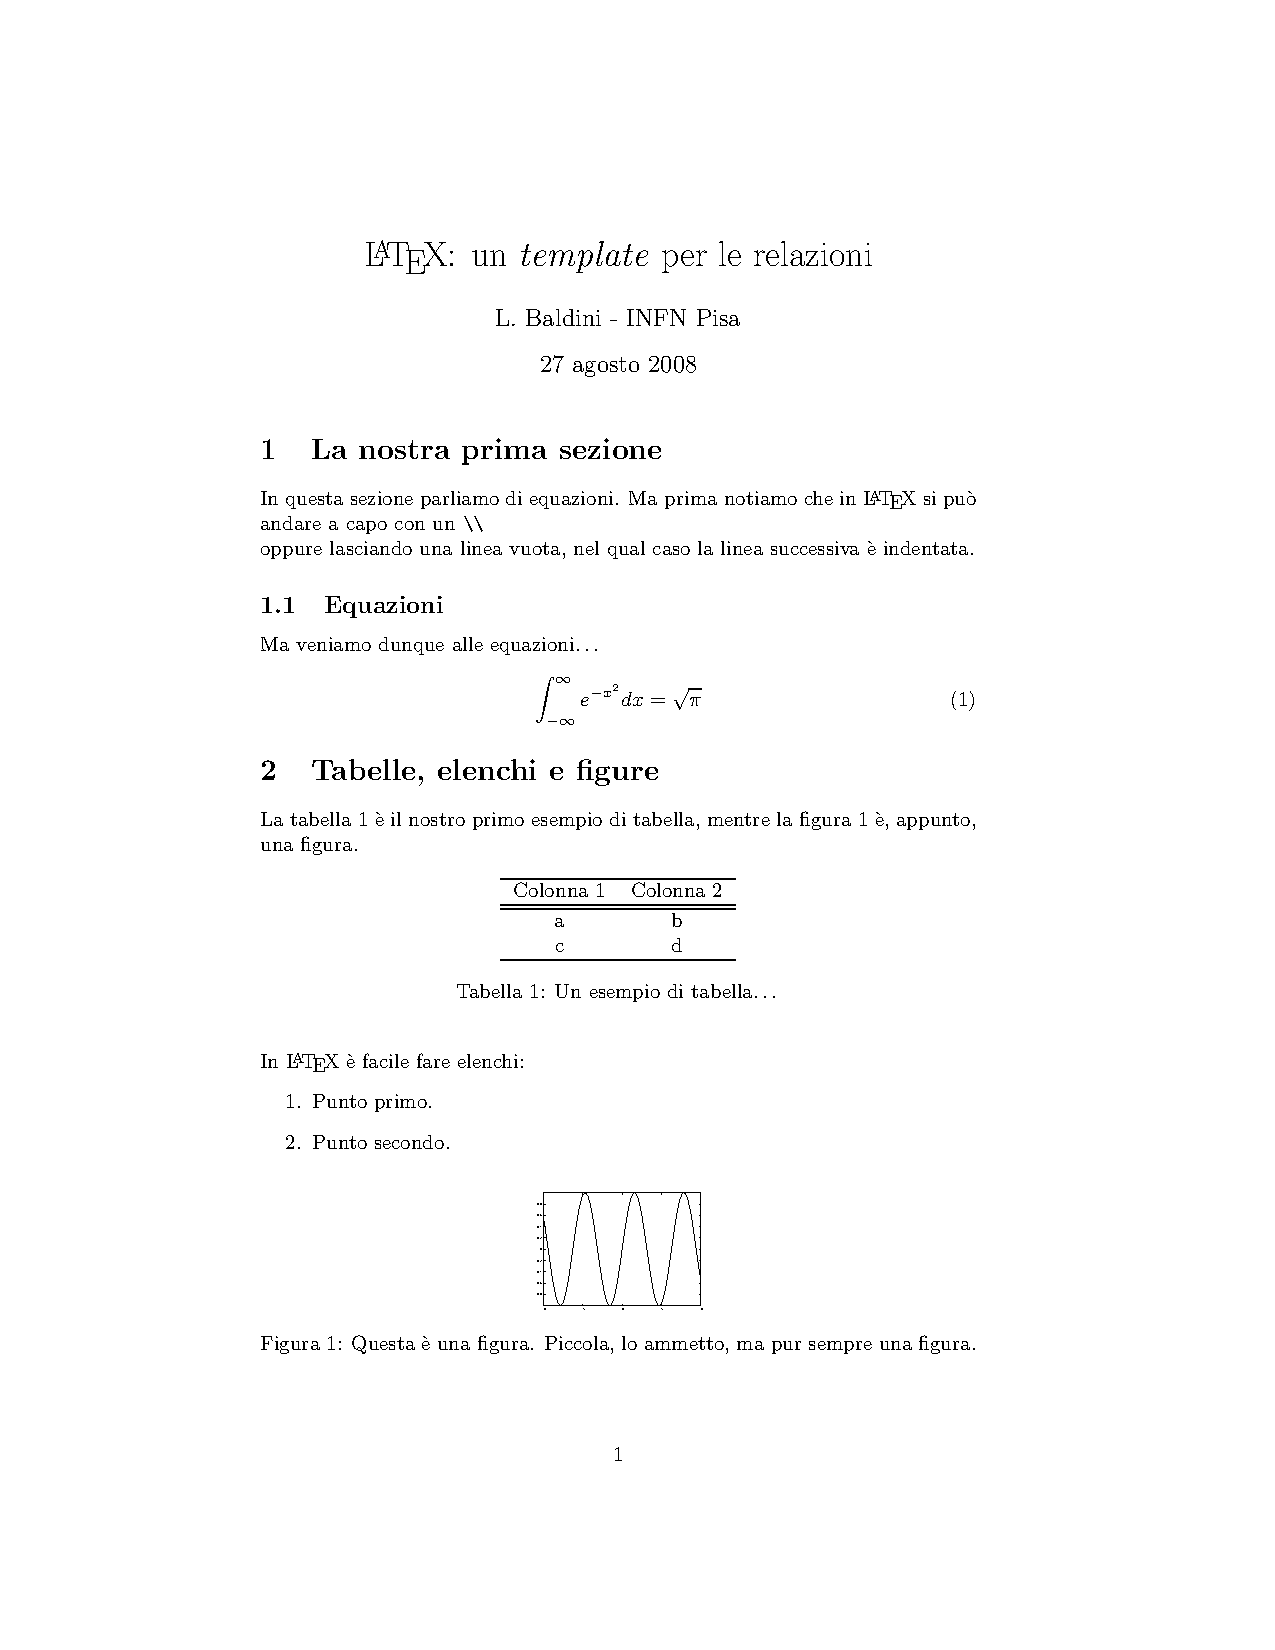
\includegraphics[width=\textwidth]{./aa_LaTeX/figure/template.pdf}}}
{Risultato della compilazione del documento \LaTeX\ di esempio.}
{fig:TemplateLaTeX}


\chapter{Simboli matematici in \LaTeX}

%\begin{table}[htbp]
%\symtable{}
%{%
%\tsym{} & \tsym{} & \tsym{} & \tsym{} & \tsym{}\\
%}
%\caption{}
%\end{table}

Le tabelle che seguono illustrano i comandi per ottenere in \LaTeX\ alcuni
tra simboli matematici pi\`u comunemente utilizzati. Ricordiamo che tutti
questi comandi sono disponibili \emph{solamente} in modalit\`a matematica---se
dovessero essere necessari all'interno del testo vanno racchiusi tra due
\cchar{\$}.

Si rimanda il lettore alla (ponderosa) guida \cite{LaTeXSym} per una lista
esaustiva dei simboli disponibili in \LaTeX.


\begin{table}[ht!]
\symtable{Lettere Greche}
{%
\tsym{alpha} & \tsym{beta} & \tsym{gamma} & \tsym{delta} & \tsym{epsilon}\\
\tsym{varepsilon} & \tsym{zeta} & \tsym{eta} & \tsym{theta} & \tsym{vartheta}\\
\tsym{gamma} & \tsym{kappa} & \tsym{lambda} & \tsym{mu} & \tsym{nu}\\
\tsym{xi} & \tsym{pi} & \tsym{varpi} & \tsym{rho} & \tsym{varrho}\\
\tsym{sigma} & \tsym{varsigma} & \tsym{tau} & \tsym{upsilon} & \tsym{phi}\\
\tsym{varphi} & \tsym{chi} & \tsym{psi} & \tsym{omega} & \\
\\
\tsym{Gamma} & \tsym{Delta} & \tsym{Theta} & \tsym{Lambda} & \tsym{Xi}\\
\tsym{Pi} & \tsym{Sigma} & \tsym{Upsilon} & \tsym{Phi} & \tsym{Psi}\\
\tsym{Omega} & & & &\\
}
\caption{Tabella dei comandi \LaTeX\ per le lettere Greche in modalit\`a
matematica.}
\end{table}


\begin{table}[b!]
\symtable{Operatori binari e di relazione}
{%
\tsym{pm} & \tsym{mp} & \tsym{times} & \tsym{div} & \tsym{circ}\\
\tsym{cdot} & \tsym{cap} & \tsym{cup} & \tsym{oplus} & \tsym{ominus}\\
\tsym{otimes} & \tsym{oslash} & \tsym{odot} &  & \\
\\
\tsym{leq} & \tsym{geq} & \tsym{ll} & \tsym{gg} & \tsym{subset}\\
\tsym{subseteq} & \tsym{supset} & \tsym{supseteq} & \tsym{in} & \tsym{ni}\\
\tsym{equiv} & \tsym{sim} & \tsym{simeq} & \tsym{approx} & \tsym{propto}\\
\tsym{cong} & \tsym{doteq} & \tsym{parallel} &  &\\
}
\caption{Tabella degli operatori binari e degli operatori di relazione pi\`u
comuni.}
\end{table}

\clearpage

\begin{table}[t!]
\symtable{Altri simboli}
{%
\tsym{ldots} & \tsym{cdots} & \tsym{vdots} & \tsym{ddots} & \tsym{forall}\\
\tsym{infty} & \tsym{hbar} & \tsym{emptyset} & \tsym{exists} & \tsym{nabla}\\
\tsym{partial} & \tsym{sum} & \tsym{prod} & \tsym{int} & \tsym{oint}\\
}
\caption{Altri simboli disponibili in \LaTeX.}
\end{table}

\rule{0pt}{0pt}

\chapter{Breve glossario di \gnuplot}

Questa appendice include alcuni dei comandi di \gnuplot\ pi\`u comunemente
usati, in combinazione con alcune tra le opzioni pi\`u utili.
Pu\`o servire da riferimento veloce durante l'elaborazione di dati.
Si rimanda comunque al capitolo \ref{chap:gnuplot} per informazioni pi\`u
dettagliate sul significato dei singoli comandi.

\begin{verbatim}
gnuplot> set output
gnuplot> set terminal x11
\end{verbatim}
\gnuplotcmd{Questi due comandi preparano \gnuplot\ ad operare nella modalit\`a
comunemente impiegata, in cui i grafici vengono rediretti sullo schermo.
\`E una buona abitudine includerli all'inizio ed alla fine di ogni macro.
Ricordiamo anche la variante per \windows\ \cchar{set terminal windows}.}

\begin{verbatim}
gnuplot> set terminal postscript
gnuplot> set output 'prova.eps'
\end{verbatim}
\gnuplotcmd{Questi comandi redirigono l'uscita su di un file postscript
denominato \cchar{prova.eps}. \`E essenziale ricordarsi di tornare allo
schermo con i due comandi precedenti, una volta scritto il file.}

\begin{verbatim}
gnuplot> help
\end{verbatim}
\gnuplotcmd{Visualizza le pagine di documentazione interattiva. Pu\`o
accettare come argomento comandi o parole chiave di \gnuplot\ su cui si
desidera avere informazioni.}

\begin{verbatim}
gnuplot> set title 'Titolo del grafico'
\end{verbatim}
\gnuplotcmd{Imposta il titolo del grafico, che \`e accettato come parametro
tra virgolette o tra apici.}

\begin{verbatim}
gnuplot> set xlabel 'x (cm)'
\end{verbatim}
\gnuplotcmd{Imposta l'etichetta di testo sull'asse delle $x$, passata come
parametro tra virgolette o apici.}

\begin{verbatim}
gnuplot> set ylabel 'y (cm)'
\end{verbatim}
\gnuplotcmd{Imposta l'etichetta di testo sull'asse delle $y$, passata come
parametro tra virgolette o apici.}

\begin{verbatim}
gnuplot> set xrange [0.5:1.5]
\end{verbatim}
\gnuplotcmd{Imposta gli estremi del grafico sull'asse delle $x$. Essi vengono
passati tra parentesi quadre, separati da due punti.}

\begin{verbatim}
gnuplot> set yrange [3:4]
\end{verbatim}
\gnuplotcmd{Imposta gli estremi del grafico sull'asse delle $y$. Funziona
esattamente come il comando precedente.}

\begin{verbatim}
gnuplot> set autoscale x
\end{verbatim}
\gnuplotcmd{Abilita l'impostazione automatica degli estremi dell'asse $x$
(che, in questo modo, si adattano ai dati).}

\begin{verbatim}
gnuplot> set autoscale y
\end{verbatim}
\gnuplotcmd{Abilita l'impostazione automatica degli estremi dell'asse $y$
(che, in questo modo, si adattano ai dati).}

\begin{verbatim}
gnuplot> unset key
\end{verbatim}
\gnuplotcmd{Elimina la legenda (se presente).}

\begin{verbatim}
gnuplot> set key
\end{verbatim}
\gnuplotcmd{Ripristina la legenda (se era stata eliminata). \`E il contrario
del comando precedente.}

\begin{verbatim}
gnuplot> set logscale x
\end{verbatim}
\gnuplotcmd{Seleziona la scala logaritmica sull'asse delle $x$.}

\begin{verbatim}
gnuplot> unset logscale x
\end{verbatim}
\gnuplotcmd{Ripristina la scala lineare sull'asse delle $x$ (se era
selezionata quella logaritmica). \`E il contrario del comando precedente.}

\begin{verbatim}
gnuplot> set logscale y
\end{verbatim}
\gnuplotcmd{Seleziona la scala logaritmica sull'asse delle $y$.}

\begin{verbatim}
gnuplot> unset logscale y
\end{verbatim}
\gnuplotcmd{Ripristina la scala lineare sull'asse delle $y$ (se era
selezionata quella logaritmica). \`E il contrario del comando precedente.}

\begin{verbatim}
gnuplot> lambda = 3.0
\end{verbatim}
\gnuplotcmd{Crea una variabile chiamata \cchar{lambda} e le assegna il valore
di $3.0$. Le variabili possono essere identificate con una qualsiasi
combinazione di lettere e numeri (purch\'e cominci con una lettera).
Questa sintassi \`e spesso usata quando si eseguono dei fit.}

\begin{verbatim}
gnuplot> print lambda
\end{verbatim}
\gnuplotcmd{Stampa sullo schermo il valore della variabile \cchar{lambda}
(che deve essere stata precedentemente definita).}

\begin{verbatim}
gnuplot> plot 'dati.txt' using 1:2
\end{verbatim}
\gnuplotcmd{Crea un grafico a partire dai dati contenuti nel file
\cchar{dati.txt}. In questo caso particolare la prima colonna \`e messa
sull'asse delle $x$, la seconda su quello delle $y$.}

\begin{verbatim}
gnuplot> plot 'dati.txt' using 1:2:3 with yerrorbars
\end{verbatim}
\gnuplotcmd{Come il comando precedente, ma la terza colonna \`e questa volta
interpretata coma colonna degli errori sull'asse delle $y$, che sono
correttamente riportati sul grafico.}

\begin{verbatim}
gnuplot> plot 'dati.txt' using 1:2:3:4 with xyerrorbars
\end{verbatim}
\gnuplotcmd{Come i due comandi precedenti, con le barre d'errore su entrambi
gli assi.}

\begin{verbatim}
gnuplot> plot 'dati.txt' using 1:2 with histeps
\end{verbatim}
\gnuplotcmd{I dati contenuti nel file \cchar{dati.txt} vengono rappresentati
sotto forma di istogramma.}

\begin{verbatim}
gnuplot> plot 'dati.txt' using 1:(($2)**2)
\end{verbatim}
\gnuplotcmd{Con questa sintassi sull'asse delle $y$ vengono rappresentati i
valori contenuta nella seconda colonna, elevati al quadrato.}

\begin{verbatim}
gnuplot> replot
\end{verbatim}
\gnuplotcmd{Esegue di nuovo l'ultimo comando \cchar{plot} che \`e stato
impartito nella \emph{shell} di \gnuplot.}

\begin{verbatim}
gnuplot> f(x) = a*sin(x)
\end{verbatim}
\gnuplotcmd{Definisce una funzione della variabile indipendente $x$ (che non
necessita di essere definita a sua volta). La funzione pu\`o poi essere usata
in un fit.}

\begin{verbatim}
gnuplot> fit f(x) 'dati.txt' using 1:2 via a
\end{verbatim}
\gnuplotcmd{Esegue un fit ai dati contenuti nel file \cchar{dati.txt} con la
funzione (precedentemente definita) $f(x)$. Il parametro $a$ \`e lasciato
libero di variare (ricordiamo che la sua inizializzazione \`e essenziale per
una corretta convergenza del fit).}

\begin{verbatim}
gnuplot> fit f(x) 'dati.txt' using 1:2:3 via a
\end{verbatim}
\gnuplotcmd{Come il comando precedente, ma in questo caso i punti $(x_i, y_i)$
sono pesati con gli errori $\Delta y_i$, contenuti nella colonna numero $3$
del file di dati.}

%\begin{verbatim}
%gnuplot>
%\end{verbatim}
%\begin{quotation}

\chapter{Un esempio di fit con \scilab}

\gnuplot\ utilizza una variante del metodo di minimo $\chi^2$ per eseguire i
fit. Il procedimento in questione \`e di tipo iterativo: si parte da una stima
iniziale dei parametri (fornita dall'utente) e si cambiano questi ultimi
fino a che il $\chi^2$ non converge ad un minimo. Questo \`e il modo in cui,
in genere, funzionano i pacchetti di analisi dati per effettuare dei fit.
In realt\`a, per lo meno nei casi pi\`u semplici, non \`e affatto complicato
scrivere dei piccoli programmi che eseguano dei fit.

\section{Minimo \texorpdfstring{$\chi^2$}{chi2} nel caso lineare}

Supponiamo di avere una serie di dati sperimentali  e di volerli fittare con
la funzione pi\`u semplice in assoluto:
\begin{equation}
f(x) = a x
\end{equation}
(abbiamo scelto una funzione puramente lineare, \`e bene notarlo, solamente
per semplicit\`a; in generale azzerare l'intercetta non \`e un'operazione
lecita).
Al solito, nell'ipotesi che gli errori sulla $x$ siano trascurabili possiamo
eseguire il fit minimizzando la quantit\`a:
\begin{equation}
S = \sum_{i=0}^n\frac{(y_i - a x_i)^2}{(\Delta y_i)^2}
\end{equation}
Nel nostro caso l'equazione da risolvere \`e:
\begin{equation}
\frac{\partial S}{\partial a} =
-2\sum_{i=0}^n\frac{(y_i - a x_i)\cdot x_i}{(\Delta y_i)^2}  = 0
\end{equation}
che conduce all'equazione per $a$:
\begin{equation}
a = \frac{\displaystyle \sum_{i=0}^n\frac{y_ix_i}{(\Delta y_i)^2}}
{\displaystyle \sum_{i=0}^n\frac{(x_i)^2}{(\Delta y_i)^2}}
\end{equation}
Notiamo, per inciso, che introducendo i vettori $n$-dimensionali:
\begin{eqnarray}
\mathbf{v} = \left(\frac{x_1}{\Delta y_1}, \frac{x_2}{\Delta y_2} \cdots 
\frac{x_n}{\Delta y_n}\right)\\\nonumber
\mathbf{w} = \left(\frac{y_1}{\Delta y_1}, \frac{y_2}{\Delta y_2} \cdots
\frac{y_n}{\Delta y_n}\right)
\end{eqnarray}
l'equazione per $a$ si pu\`o scrivere in forma compatta come:
\begin{equation}
a = \frac{\mathbf{v} \cdot \mathbf{w}}{\mathbf{v} \cdot \mathbf{v}}
\end{equation}
in cui il puntino sta ad indicare l'usuale prodotto scalare tra vettori.

\section{Implementare il fit con \scilab}

A questo punto eseguire il fit \`e una cosa semplice: basta prendere i dati
ed eseguire, nella giusta sequenza, i prodotti, le divisioni e le somme
necessarie a calcolare $a$ secondo l'equazione scritta sopra.
Una calcolatrice va benissimo, ma il tutto si pu\`o fare in modo pi\`u
efficiente (specialmente nel caso si abbia un gran numero di dati)
scrivendo un piccolo programma.
Qualsiasi linguaggio di programmazione pu\`o servire egregiamente allo scopo;
noi proveremo a farlo con il pacchetto \emph{software} \scilab, che offre
tutta una serie di funzioni utili per maneggiare matrici e vettori.

\scilab\ si lancia dalla \emph{shell} con il comando:
\begin{verbatim}
>scilab
\end{verbatim}
La prima cosa che dobbiamo fare \`e importare entro scilab la nostra matrice
di dati, che chiameremo \cchar{M}. Supponendo che il nostro \emph{file} si
chiami \cchar{LeggeOraria.txt}, useremo il comando di \scilab\ \cchar{read}
come segue:
\begin{verbatim}
scilab>[M] = read('LeggeOraria.txt', 6, 3)
[M] =
|  5   10.1   2.0 |
| 10   17.8   1.5 |
| 15   26.6   1.5 |
| 20   32.8   2.0 |
| 25   40.2   2.5 |
| 30   47.4   2.0 |
scilab>
\end{verbatim}
Essenzialmente questo significa: leggiamo il \emph{file}
\cchar{LeggeOraria.txt} ed estraiamo una matrice di sei righe e tre colonne
che chiamiamo \cchar{M} e che da questo momento \`e disponibile in memoria
per effettuare le operazioni desiderate; ad ogni passo \scilab\ dovrebbe
stampare sullo schermo ci\`o che abbiamo appena fatto, che \`e utile per
verificarne la correttezza.

\caution{\scilab\ non ama i commenti (le righe precedute da \cchar{\#}, che
invece non creavano problemi a \gnuplot) per cui dobbiamo avere la precauzione
di cancellarle dal \emph{file} contenente i dati, prima di eseguire il
comando.}

A questo punto dobbiamo estrarre dalla matrice i vettori che ci interessano,
cio\`e quello delle $x$, quello delle $y$ e quello degli errori sulla $y$.
Il modo per farlo (con ovvio significato dei termini) \`e:
\begin{verbatim}
scilab>[x] = M(:, 1)
[x] =
|  5  |
| 10  |
| 15  |
| 20  |
| 25  |
| 30  |
scilab>[y] = M(:, 2)
| 10.1 |
| 17.8 |
| 26.6 |
| 32.8 |
| 40.2 |
| 47.4 |
scilab>[dy] = M(:,3)
| 2.0 |
| 1.5 |
| 1.5 |
| 2.0 |
| 2.5 |
| 2.0 |
scilab>
\end{verbatim}
Cio\`e: definiamo il vettore $x$ come la prima colonna della matrice \cchar{M},
il vettore $y$ come la seconda colonna e $dy$ come la terza colonna.
Costruiamo quindi i vettori $\mathbf{v}$ e $\mathbf{w}$ definiti nel paragrafo
precedente:
\begin{verbatim}
scilab>v = x./dy
scilab>w = y./dy
scilab>
\end{verbatim}
(notare che l'operatore \cchar{./} \`e quello che consente, dentro \scilab,
di eseguire la divisione membro a membro di due vettori).
Non ci resta che eseguire i prodotti scalari per calcolare $a$:
\begin{verbatim}
scilab>(v'*w)/(v'*v)
\end{verbatim}
(l'apostrofo \cchar{'} indica il vettore trasposto, dopo di che il prodotto
scalare si esegue con l'usuale simbolo di moltiplicazione); \scilab\ dovrebbe
visualizzare sullo schermo il valore del parametro cercato.


% Bibliografia e colophon.
\begin{thebibliography}{100}

\addcontentsline{toc}{chapter}{Bibliografia}

\bibitem{Bevington}
\book{Philip~R.~Bevington, D.~Keith~Robinson}
{Data Reduction and Error Analysis for the Physical Sciences}
{McGraw~Hill, Third Edition, 2003}

\bibitem{DelPrete}
\pbook{Tarcisio~Del~Prete}
{Methods of Statistical Data Analysis in High Energy Physics}
{http://www.pi.infn.it/atlas/documenti/note/statistica.ps.gz}

\bibitem{Taylor}
\book{John~R.~Taylor}
{Introduzione all'analisi degli errori}
{Zanichelli Editore, Seconda Edizione, 2000}

\bibitem{Loreti}
\pbook{Maurizio~Loreti}
{Teoria degli errori e fondamenti di statistica (introduzione alla fisica
sperimentale)}
{http://wwwcdf.pd.infn.it/labo/INDEX.html}

\bibitem{Brownlee}
\book{Kenneth~A.~Brownlee}
{Statistical theory and methodology in science and engineering}
{Wiley publications in applied statistics, Second Edition, 1984}

\bibitem{Cramer}
\book{Harald~Cramer}
{Mathematical Methods of Statistics}
{Princeton University Press, Paperback Edition, 1999}

\bibitem{Arley}
\book{Niels~Arley, K.~Rander~Buch}
{Introduction to the theory of probability and statistics}
{Wiley~\&~Sons, 1950}

\bibitem{Kyker}
\article{Granvil~C.~Kyker Jr.}
{Am. J. Phys. 51 (9), 852 (1983)}

\bibitem{McGovern}
\article{Wayne~E.~McGovern}
{Am. J. Phys. 60 (10), 943 (1992)}

\bibitem{Lafleur}
\book{M.~S.~Lafleur, P.~F.~Hinrichsen, P.~C.~Landry, R.~B.~Moore}
{The Poisson Distribution}
{Physics Teacher 10, 314 (1972)}

\bibitem{McCormick}
\book{John.~M.~Mc~Cormick, Mario~G.~Salvadori}
{Numerical Methods in Fortran}
{Prentice-Hall, 1964}

\bibitem{Linux1}
\pbook{Lars~Wirzenius}
{Guida dell'amministratore di sistema \linux}
{ftp://ftp.pluto.it/pub/pluto/ildp/guide/sag/sag.pdf}

\bibitem{Linux2}
\pbook{Larry~Greenfield}
{\linux\ guida dell'utente}
{ftp://ftp.pluto.it/pub/pluto/ildp/guide/Guida-Utente/Guida-Utente.pdf}

\bibitem{latex-homepage}
\homepage{Home page di \LaTeX}
{http://www.latex-project.org}

\bibitem{guit}
\homepage{Home page del Gruppo utilizzatori Italiani di \TeX}
{http://www.guit.sssup.it}

\bibitem{LaTeX}
\pbook{Marc~Baudoin}
{Impara {\LaTeX}! (\ldots e mettilo da parte)}
{http://www.mat.uniroma1.it/centro-calcolo/manuali/impara\_latex.pdf}

\bibitem{LaTeXNSS}
\pbook{Tobias~Oetiker}
{The Not So Short Introduction to \LaTeX2e}
{http://www.ctan.org/tex-archive/info/lshort/english/lshort.pdf}

\bibitem{LaTeXSym}
\pbook{Scott~Pakin}
{The Comprehensive \LaTeX\ Symbol List}
{www.ctan.org/tex-archive/info/symbols/comprehensive/symbols-a4.pdf}

\bibitem{gnuplot-homepage}
\homepage{Home page di \gnuplot}
{http://www.gnuplot.info}

\bibitem{scilab-homepage}
\homepage{Home page di scilab}
{http://www.scilab.org}

\bibitem{sourceforge-homepage}
\homepage{Home page di sourceforge}
{http://sourceforge.net}

\bibitem{gnu-homepage}
\homepage{Home page di {\sc gnu} ({\sc gnu}'s Not Unix)}
{http://www.gnu.org}

\bibitem{pyhton-homepage}
\homepage{Home page di python}
{http://www.python.org}

\end{thebibliography}

\caution{Tutti i link a pagine web contenuti tra le indicazioni bibliografiche
erano correttamente funzionanti la mattina del 14 Agosto 2007.}

\thispagestyle{empty}

\hfill

\vfill

\section*{Colophon}
\pdfbookmark[0]{Colophon}{colophon}

Questo lavoro \`e stato realizzato con \LaTeXe\ sulla distribuzione di
\linux{} Fedora 11. Tutti i grafici sono stati realizzati con \gnuplot{}
versione 4.2 \emph{patchlevel} 2. Le tavole numeriche sono state generate
utilizzando pyROOT versione 5.18.00.


\printindex

\end{document}
